% ****** Start of file apssamp.tex ******
%
%   This file is part of the APS files in the REVTeX 4.1 distribution.
%   Version 4.1r of REVTeX, August 2010
%
%   Copyright (c) 2009, 2010 The American Physical Society.
%
%   See the REVTeX 4 README file for restrictions and more information.
%
% TeX'ing this file requires that you have AMS-LaTeX 2.0 installed
% as well as the rest of the prerequisites for REVTeX 4.1
%
% See the REVTeX 4 README file
% It also requires running BibTeX. The commands are as follows:
%
%  1)  latex apssamp.tex
%  2)  bibtex apssamp
% https://www.overleaf.com/project/5b0c51828e746f209754cf04 3)  latex apssamp.tex
%  4)  latex apssamp.tex
%
\documentclass[%
 reprint,
%superscriptaddress,
%groupedaddress,
%unsortedaddress,
%runinaddress,
%frontmatterverbose, 
%preprint,
%showpacs,preprintnumbers,
%nofootinbib,
%nobibnotes,
%bibnotes,
 amsmath,amssymb,
 aps,
%pra,
%prb,
%rmp,
%prstab,
%prstper,
%floatfix,
]{revtex4-1}

\usepackage{tabularx}                                 % tables with automatic width calculation
\usepackage{graphicx}% Include figure files
\usepackage{xcolor}
\usepackage{hepunits}
\usepackage{dcolumn}% Align table columns on decimal point
\usepackage{bm}% bold math
%\usepackage{hyperref}% add hypertext capabilities
%\usepackage[mathlines]{lineno}% Enable numbering of text and display math
%\linenumbers\relax % Commence numbering lines

%\usepackage[showframe,%Uncomment any one of the following lines to test 
%%scale=0.7, marginratio={1:1, 2:3}, ignoreall,% default settings
%%text={7in,10in},centering,
%%margin=1.5in,
%%total={6.5in,8.75in}, top=1.2in, left=0.9in, includefoot,
%%height=10in,a5paper,hmargin={3cm,0.8in},
%]{geometry}



%%%%%%%%%%%%%%%%%%%%%%%%%%%%%%%%%%%%%%%%%%%%%%%%%%%%%%%%%%%%%%%%%%%%
%%  basic formatting macros:
%%%%%%%%%%%%%%%%%%%%%%%%%%%%%%%%%%%%%%%%%%%%%%%%%%%%%%%%%%%%%%%%%%%

%%  single-line equations:

\def\beq{\begin{equation}}
\def\eeq#1{\label{#1}\end{equation}}
\def\eeqn{\end{equation}}

%%  multiple-line equations  (use \CR as the carriage return):

\newenvironment{Eqnarray}%
   {\arraycolsep 0.14em\begin{eqnarray}}{\end{eqnarray}}
\def\beqa{\begin{Eqnarray}}
\def\eeqa#1{\label{#1}\end{Eqnarray}}
\def\eeqan{\end{Eqnarray}}
\def\CR{\nonumber \\ }

%%  reference to an equation number:

\def\leqn#1{(\ref{#1})}

%%%%%%%%%%%%%%%%%%%%%%%%%%%%%%%%%%%%%%%%%%%%%%%%%%%%%%%%%%%%%%%%%%%%%%%%

%%  bibliographic entries   (use this or the SPIRES LaTeX output)

%%   Journal or bibliographic formatting macros are obsolete!
%%   The SLAC/SPIRES database supplies properly formatted citations;
%%      click on  LaTeX(US) or LaTeX(EU)   

%%%%%%%%%%%%%%%%%%%%%%%%%%%%%%%%%%%%%%%%%%%%%%%%%%%%%%%%%%%%%%%%%%%%%%%%%

%%  sizing and bars

\def\st{\scriptstyle}
\def\sst{\scriptscriptstyle}

\def\overbar#1{\overline{#1}}
\let\littlebar=\bar
\let\bar=\overbar

\def\subscr#1{{\mbox{\scriptsize #1}}}


%%%%%%%%%%%%%%%%%%%%%%%%%%%%%%%%%%%%%%%%%%%%%%%%%%%%%%%%%%%%%%%%%%%%%%%%%

%%  text-mode macros:

\def\etal{{\it et al.}}
\def\ie{{\it i.e.}}
\def\eg{{\it e.g.}}
\def\etc{{\it etc.}}

\def\ifb{ fb$^{-1}$ }
\def\iab{ ab$^{-1}$ } 

%%%%%%%%%%%%%%%%%%%%%%%%%%%%%%%%%%%%%%%%%%%%%%%%%%%%%%%%%%%%%%%%%%%%%%%%%%

%%  expectation values:

\def\VEV#1{\left\langle{ #1} \right\rangle}
\def\bra#1{\left\langle{ #1} \right|}
\def\ket#1{\left| {#1} \right\rangle}
\def\vev#1{\langle #1 \rangle}

%%%%%%%%%%%%%%%%%%%%%%%%%%%%%%%%%%%%%%%%%%%%%%%%%%%%%%%%%%%%%%%%%%%%%%%%%

%% relation symbols

\def\lsim{\mathrel{\raise.3ex\hbox{$<$\kern-.75em\lower1ex\hbox{$\sim$}}}}
\def\gsim{\mathrel{\raise.3ex\hbox{$>$\kern-.75em\lower1ex\hbox{$\sim$}}}}

\def\Im{{\rm Im}}
\def\Re{{\rm Re}}

%%%%%%%%%%%%%%%%%%%%%%%%%%%%%%%%%%%%%%%%%%%%%%%%%%%%%%%%%%%%%%%%%%%%%%%%%%%%%%
%%  caligraphic letters (for matrix elements, luminosity, etc.)

\def\D{{\cal D}}
\def\L{{\cal L}}
\def\M{{\cal M}}
\def\O{{\cal O}}
\def\W{{\cal W}}

%%%%%%%%%%%%%%%%%%%%%%%%%%%%%%%%%%%%%%%%%%%%%%%%%%%%%%%%%%%%%%%%%%%%%

%%  matrix operations and fractions:

\def\One{{\bf 1}}
\def\hc{{\mbox{\rm h.c.}}}
\def\tr{{\mbox{\rm tr}}}
\def\half{\frac{1}{2}}
\def\thalf{\frac{3}{2}}
\def\third{\frac{1}{3}}
\def\tthird{\frac{2}{3}}

\def\del{\partial}
\def\Dslash{\not{\hbox{\kern-4pt $D$}}}
\def\dslash{\not{\hbox{\kern-2pt $\del$}}}

%%%%%%%%%%%%%%%%%%%%%%%%%%%%%%%%%%%%%%%%%%%%%%%%%%%%%%%%%%%%%%%%%%%%%%%%%%%%%

%%  high-energy physics terminology:

\def\Pl{{\mbox{\scriptsize Pl}}}
\def\eff{{\mbox{\scriptsize eff}}}
\def\CM{{\mbox{\scriptsize CM}}}
\def\GUT{{\mbox{\scriptsize GUT}}}
\def\BR{\mbox{\rm BR}}
\def\ee{e^+e^-}
\def\sstw{\sin^2\theta_w}
\def\cstw{\cos^2\theta_w}
\def\mz{m_Z}
\def\gz{\Gamma_Z}
\def\mw{m_W}
\def\mt{m_t}
\def\gt{\Gamma_t}
\def\mh{m_h}
\def\gmu{G_\mu}
\def\GF{G_F}
\def\alphas{\alpha_s}
\def\msb{{\bar{\scriptsize M \kern -1pt S}}}
\def\lmsb{\Lambda_{\msb}}
\def\drb{{\bar{\scriptsize D \kern -1pt R}}}
\def\ELER{e^-_Le^+_R}
\def\EREL{e^-_Re^+_L}
\def\ELEL{e^-_Le^+_L}
\def\ERER{e^-_Re^+_R}
\def\eps{\epsilon}

%%%%%%%%%%%%   Roman in math mode

\def\GeV{ \mbox{GeV} }
\def\TeV{  \mbox{TeV} } 
\def\MeV{ \mbox{MeV} } 


%%%%%%%%%%%%%%%%%%%%%%%%%%%%%%%%%%%%%%%%%%%%%%%%%%%%%%%%%%%%%%%%%%%%%

% spinor products 

\def\spa#1#2{\langle #1 #2 \rangle}
\def\spb#1#2{[ #1 #2 ]}
\def\apb#1#2#3{\langle #1 #2 #3 ]}
\def\bpa#1#2#3{[ #1 #2 #3 \rangle}

%%%%%%%%%%%%%%%%%%%%%%%%%%%%%%%%%%%%%%%%%%%%%%%%%%%%%%%%%%%%%%%%%%%%%%%%%%%%%

%%  supersymmetry:

\def\ch#1{\widetilde\chi^+_{#1}}
\def\chm#1{\widetilde\chi^-_{#1}}
\def\neu#1{\widetilde\chi^0_{#1}}
\def\s#1{\widetilde{#1}}

%%%%%%%%%%%%%%%%%%%%%%%%%%%%%%%%%%%%%%%%%%%%%%%%%%%%%%%%%%%%%%%%%%%%%%%%%%%%%5

\makeatletter
\def\section{\@startsection{section}{0}{\z@}{5.5ex plus .5ex minus
 1.5ex}{2.3ex plus .2ex}{\large\bf}}
\def\subsection{\@startsection{subsection}{1}{\z@}{3.5ex plus .5ex minus
 1.5ex}{1.3ex plus .2ex}{\normalsize\bf}}
\def\subsubsection{\@startsection{subsubsection}{2}{\z@}{-3.5ex plus
-1ex minus  -.2ex}{2.3ex plus .2ex}{\normalsize\sl}}

%%%%%%%%%%%%%%%%%%%%%%%%%%%%%%%%%%%%%%%%%%%
% small size table and figure captions %
%%%%%%%%%%%%%%%%%%%%%%%%%%%%%%%%%%%%%%%%%%%
\renewcommand{\@makecaption}[2]{%
   \vskip 10pt
   \setbox\@tempboxa\hbox{\small #1: #2}
   \ifdim \wd\@tempboxa >\hsize     % IF longer than one line:
       \small #1: #2\par          %   THEN set as ordinary paragraph.
     \else                        %   ELSE  center.
       \hbox to\hsize{\hfil\box\@tempboxa\hfil}
   \fi}

%%%%%%%%%%%%%%%%%%%%%%%%%%%%%%%%%%%%%%%%%%%%%%%%%%%%%%%%%%%%%%%%%%%%
%%%%%%%%%%%%%%%
\makeatother


% this is a very convenient small macropackage, which was used for previous Physics WG documents.  Please use it here rather than inputing your own larger package --  MEP

\newcommand {\sub}[1]{\ensuremath{_{\mathrm{#1}}}}
\newcommand {\siunit}[2]{\ensuremath{#1\,{\mathrm{#2}}}}
\newcommand {\num}[1]{\ensuremath{#1}}


\begin{document}

\preprint{LCCPEB---}

\title{The International Linear Collider \\ A Global Project}% Force line breaks with \\
\thanks{Version 1.3}%

\author{Jim Brau}
% \altaffiliation[Also at ]{Physics Department, XYZ University.}%Lines break automatically or can be forced with \\
\author{etal}%
 \email{Second.Author@institution.edu}
\affiliation{%
 Authors' institution and/or address\\
% This line break forced with \textbackslash\textbackslash
}%

\collaboration{Linear Collider Collaboration}%\noaffiliation

\date{\today}% It is always \today, today,
             %  but any date may be explicitly specified

\begin{abstract}
Input from the International Linear Collider community for the European Strategy Update: supplementary material

\end{abstract}

\pacs{Valid PACS appear here}% PACS, the Physics and Astronomy
                             % Classification Scheme.
%\keywords{Suggested keywords}%Use showkeys class option if keyword
                              %display desired
\maketitle

%\tableofcontents

\section{\label{sec:intro}Introduction}
   5 pages Brau + Peskin
   
   %  Introduction to the document
While the Standard Model (SM) is a highly successful theory of
the fundamental interactions, shortcomings are known and new physics
is required to address them.  A central focus of particle physics
now involves
searching for this physics in the form
of new particles and/or new interactions.  The SM is theoretically
 self-consistent, but it does not explain dark matter or dark energy
 as observed in the cosmos,
and it cannot explain the excess of matter over antimatter.   It does
not address the mass scale of quarks, leptons, and gauge 
bosons, which is significantly lower than the Planck scale.   
Specifically, it does not explain
the large mass ratios among the SM particles.   
These and other considerations provide a compelling motivation
for the search, while the success of the SM indicates
the degree of challenge this search faces.
The first evidence for the new physics
may appear in deviations to SM predictions 
in high-precision measurements. 
Such evidence could be the first clues to what lies beyond the SM.

The SM was completed in 2012 with the discovery of the Higgs boson.
Its role in electroweak symmetry-breaking and the mechanism of
mass generation for all known fundamental particles places the Higgs boson
in a central role for the SM.  Its properties are precisely
specified by the SM, making precision measurements of these
properties particular sensitive to the new physics.
 
The Higgs boson properties are the first significant goal for
experimentation at the International Linear Collider (ILC).
A large, world-wide community of physicists is working to realise
the exceptional physics program
of electron-positron collisions with the ILC.
The ILC has been designed to optimally address the
central physics issues described above.  The ILC's unprecedented, model-independent measurement precision
provides a leap in sensitivity to the deviations.
At the first stage of the ILC the well-defined SM specifications
of the Higgs boson properties will be tested in great detail.
These measurements 
discriminate between the SM and many proposed extensions of the SM.
The ILC will be sensitive to invisible and other exotic Higgs decays,
testing new physics models including models of dark
matter.  With no new particles beyond the SM having been
discovered at the LHC, the search for new physics through
these high-precision studies is urgent and compelling. 
ILC will also test other SM expectations 
and search for direct evidence of new physics
in pair-production of weakly interacting particles.

Using an $\ee$ linear collider to explore this scientific arena
brings several excellent experimental properties to the
challenge of the measurements.
The ILC has a well-defined, adjustable centre-of-mass energy 
in the production and faces a small background level.
In addition, both colliding beams offer high levels of polarisation
that introduces additional observables opening access to
important properties, such as
the electroweak couplings of right-handed
fermions, 
which are largely unconstrained today.
After operation at the starting energy,
the linear collider can undergo an energy upgrade in a fairly
straightforward way; this will expand the list of physics processes that
can be studied with precision, providing additional pathways
to finding evidence of the new physics.
These energy upgrades can access the properties of the top quark,
including top-quark Yukawa coupling, and to the Higgs self-coupling.
For centre-of-mass energies above the top-quark pair-production threshold
the ILC becomes a top-quark factory.
As the energy rises, new BSM particles of mass up to half
the centre-of-mass energy will be searched for.
Even higher $Z'$ mass reach of up to 10 TeV
 is achieved through its 
mixing with the  $Z$ in the intermediate state.
Because of this upgrade capability and the unique reach, the ILC may
continue to be a leading discovery machine in the 
world of particle physics for decades.
This method of searching for 
new physics beyond the SM is orthogonal to and complements 
the LHC physics program.


The ILC technology is mature and construction-ready, following
more than twenty years of a worldwide-coordinated 
research program to develop the technology required.
As the linear collider technology was developing
decades ago,
committees of   the International Committee for Future Accelerators
(ICFA) guided its successive stages.
In the mid-1990's various technology options to
realise a high-energy linear collider were emerging. 
ICFA asked the 
Linear Collider Technical Review Committee to develop a standardised
way to  compare  these  technologies based on their parameters, such as
power consumption and luminosity. A second
review panel was organised by ICFA in 2002;
it concluded that both warm and cold technologies had
developed to the point where either could be the basis for a
high energy linear
collider. In 2004, the  International Technology Review Panel
(ITRP) was charged by ICFA to recommend an option that could focus the
worldwide R\&D effort.  This panel chose the  superconducting
radiofrequency technology (SCRF), in a large part due to its
energy efficiency and potential for broader applications. 


The collider design is the result of nearly twenty years of
R\&D. The heart of the ILC, the SCRF cavities, is based on
pioneering work of the TESLA Technology Collaboration. Other aspects of the 
technology
emerged from the R\&D carried out for the JLC/GLC and NLC projects,
which were based on room-temperature accelerating structures. 
The effort to design and
establish the technology for the linear collider culminated in the
publication of the Technical Design Report (TDR) for the International
Linear Collider (ILC) in 2013~\cite{Behnke:2013xla}. 
Twenty-four hundred (2400) scientists, from 48 countries and 392 institutes and university
groups,
 signed the TDR,
 that presented optimised collider and detector designs, and associated 
physics analyses. 
From
2005 to the publication of the TDR, the
design of the ILC accelerator was conducted under the mandate of ICFA
as a worldwide
international collaboration, the Global Design Effort (GDE). 
Since 2013, ICFA has placed the  international activities for both the ILC and CLIC
projects under a single organisation, 
the Linear Collider Collaboration (LCC),

So, the ILC proposal
is supported by extensive R\&D and prototyping. The successful construction and
operation 
of the European XFEL at DESY provides
confidence both in the high reliability of the basic
technology and in the reliability of its performance and cost in 
industrial realisation.   
Some specific optimisations and technological choices remain.
But the ILC is now ready to move forward to construction. 


With knowledge of the mass of the Higgs boson, it was established in 2012 that the
linear collider could start its ambitious physics program with an initial centre-of-mass energy of 250 GeV at a cost
reduced from the TDR. A revised design of the ILC, the ILC250, was
thus  presented~\cite{Evans:2017rvt} retaining the final-focus and
beam-dump capability to extend the centre-of-mass energy to higher
energies. Advances in the theoretical understanding of the impact of precision
measurements at the 
 ILC250 have justified that this operating point already gives
 substantial 
sensitivity to physics beyond the SM~\cite{Barklow:2017suo,Fujii:2017vwa}. 
 The cost estimate for ILC250 
  is similar in scale to the LHC project cost.


In its current
form, the ILC250 is a $250\,{\mathrm{GeV}}$ centre-of-mass energy
(extendable up to $1\,{\mathrm{TeV}}$) linear $e^+e^-$ collider, based
on $1.3\,{\mathrm{GHz}}$ SCRF
cavities. It is designed to achieve a luminosity of $1.35\cdot
10^{34}~{\mathrm{cm}}^{-2}{\mathrm{s}}^{-1}$ and provide an integrated
luminosity of $400\,{\mathrm{fb}}^{-1}$ in the first four years of
running. The electron beam will be polarised to $80\,\%$, and the baseline plan includes an 
undulator-based
positron source which will  deliver
$30\,\%$ positron  polarisation. 


The experimental community has developed
designs for two complementary detectors, ILD and SiD, 
as described in \cite{Behnke:2013lya}. These detectors are designed to 
optimally address the
ILC physics goals, with complementary approaches. One detector is based on
TPC tracking (ILD) and one on silicon tracking (SiD).
Both employ particle flow calorimetry based on
calorimeters with unprecedented fine segmentation.
As with the collider technology, 
extensive R\&D and prototyping gives confidence that the
unprecedented,
high-precision detectors envisaged to achieve the 
physics programme can be realised.
An extensive course of
prototyping underlies the estimates of full-detector performance 
and cost.  
The detector R\&D program leading to these designs
has 
contributed a number of advances in 
detector capabilities with applications well beyond the linear
collider program. 
As for the
collider, optimisations and final technological choices 
will need to be completed in the next few years. 

There is broad interest in Japan to host the
international effort to realise the ILC project.  
This interest has been growing over many years.
Political entities are promoting the plan to host,
including the Japanese Diet,
a large industrial consortium (AAA),
and the representatives of the particle physics community (JAHEP).
Detailed reviews in Japan of the many aspects of the
project is nearing a conclusion.
First,
since 2013 the MEXT ministry has examined the ILC project in
great detail, including the aspect of risk minimisation.
This concluded when
MEXT's ILC Advisory Panel released 
its report~\cite{AdvPanel} on July 4, 2018, summarising the
studies of the several working groups (WG) that
reviewed 
a broad range of aspects of the ILC.  The most recent studies include
a specific review of the scientific merit and the technical design for the ILC250. 
The  Physics WG scrutinised the scientific merit of the ILC250,
leading to their strong and positive statement on the importance of
the ILC250 to 
measure precisely the couplings of the Higgs boson \cite{AdvPanel}.
The TDR WG reviewed issues addressed in the Technical Design Report
and the ILC250 design, including the  cost estimate and technical feasibility.  
Other working groups of the MEXT review commented on manpower needs, 
organisational aspects, and the experience of previous large projects.
The report of the ILC Advisory Panel was followed by the beginning of
deliberations in a committee and technical working group 
established by the Science Council of Japan (SCJ),
the second stage of the review process. 
The SCJ review is nearing completion.
  The Japanese government is preparing for the next step,
a decision on hosting, and to move to the next phase of international negotiations.
It is an important aspect of the discussions of the ILC in Japan that the
ILC is seen as global project that will foster exchange between Japan
and other nations.   Thus, the  
scientific interest and political engagement of partner countries is a
major 
concern for the Japanese authorities.  
Another independent committee (ILC Liaison Council),
led by leaders of the Liberal Democratic 
Party, the majority party in the Diet,  has now 
convened to encourage the national government to proceed with the ILC.
The project could start within a few years. 
The initial phase of a potential timeline 
would last about four years to obtain
 international agreements, prepare construction and form 
 the requisite international
collaboration; the construction phase would need nine years.


This report details the current status of this effort, describing
the physics reach, the technological maturity of the accelerator,
detector, and software/computing designs,
plus a discussion on the further steps 
 needed to realise the project.
 The ILC accelerator design and technology is described
 in Section \ref{sec:ilc}.  Many aspects of the development of
 the SCRF is presented, as well as general aspects
 of the machine. Luminosity and energy upgrade options are
 discussed, as well as civil engineering plans, including site
 specific details, and the cost and schedule estimates.
 Section \ref{sec:runscenarios}  presents the current
 thinking about the operations of the ILC, estimating 
 collection of integrated luminosity.
 Section \ref{sec:physics} details the physics case for the ILC.
 This includes an overview of the significance of the Higgs boson 
 as a tool for searching for BSM physics,  
 the details of the Higgs boson studies at the ILC, 
 complementarity to the LHC, and examples of other physics
 of interest including SM fermion pair-production and
 new particle pair production.  Section \ref{sec:detectors}
 provides detailed descriptions of the ILC detector designs
 that have been developed by the community,
 through detector R\&D and prototyping, and used as detector
 models to show the simulated performance on the various
 physics channels. Section \ref{sec:software}
 summarises the computing needs of the ILC program,
 including software.    Section \ref{sec:higgs}
 gives a description of many physics simulations
 that have been completed based on the detectors of
 Section \ref{sec:detectors} to understand the
 reach of the physics program.
 The possible ILD physics program for energies
 beyond 250 GeV are described in
 Section \ref{sec:searches}.



   
\section{\label{sec:ilc}ILC Machine Design}

  15 pages B. List + Michizono
  
% CHAPTER ON ILC MACHINE

%{\it Status: Feb 12, 2019}  - revised by MEP

The International Linear Accelerator (ILC) is a $250\,{\mathrm{GeV}}$ (extendable up to $1\,{\mathrm{TeV}}$) linear $e^+e^-$ collider, based on $1.3\,{\mathrm{GHz}}$ superconducting radio-frequency (SCRF) cavities.
It is designed to  achieve a luminosity of $1.5\cdot 10^{34}~{\mathrm{cm}}^{-1}{\mathrm{s}}^{-1}$ and provide an integrated luminosity of $350\,{\mathrm{fb}}^{-1}$ in the first four years of running.
The electron beam will be polarised to $80\,\%$, and positrons with $30\,\%$ polarization will be provided if the undulator based positron source concept is employed. 

Its parameters have been set by physics requirements first outlined in 2003,
updated in 2006, and thoroughly discussed over many years with the physics user community. 
After the discovery of the Higgs boson it was decided that an initial energy of $250\,{\mathrm{GeV}}$ provides the opportunity for a precision physics programme at a reasonable initial cost~\cite{Evans:2017rvt}.
Some relevant parameters are given in Tab.~\ref{tab:ilc-params}.

\begin{table*}[tbhp]
\begin{tabular}{lcccccc}
Quantity & Symbol & Unit & Initial & TDR &  \multicolumn{2}{c}{Upgrades} \\
\hline
Centre of mass energy & $\sqrt{s}$ & ${\mathrm{GeV}}$ & $250$ & $250$ & $500$ & $1000$ \\
Luminosity & \multicolumn{2}{c}{${\mathcal{L}}$ ~~~~$10^{34}{\mathrm{cm^{-2}s^{-1}}}$} & $1.35$ & $0.75$ & $1.8$ & $4.9$ \\
Polarisation for $e^- (e^+)$ & $P\sub{-} (P\sub{+})$ & & ~$80\,\% (30\,\%)$~ &  ~$80\,\% (30\,\%)$~ &  ~$80\,\% (30\,\%)$~ &  ~$80\,\% (20\,\%)$~  \\
Repetition frequency &$f\sub{{rep}}$ & ${\mathrm{Hz}}$  & $5$ & $5$ & $5$ & $4$ \\
Bunches per pulse  &$n\sub{{bunch}}$ & 1  & $1312$ & $1312$ & $1312$ & $2450$ \\
Bunch population  &$N\sub{{e}}$ & $10^{10}$ &$2$ & $2$ & $2$ & $1.74$ \\
Linac bunch interval & $\Delta t\sub{{b}}$ & ${\mathrm{ns}}$ & $554$ & $554$ & $554$ & $366$ \\
Beam current in pulse & $I\sub{{pulse}}$ & ${\mathrm{mA}}$& $5.8$ & $5.8$ & $5.8$ & $7.6$  \\
Beam pulse duration  & $t\sub{{pulse}}$ & ${\mathrm{\mu s}}$ & $727$ & $727$ & $727$ & $897$ \\
Average beam power  & $P\sub{{ave}}$   & ${\mathrm{MW}}$ & $5.3$ & $5.3$ & $10.5$  & $27.2$ \\  
Norm. hor. emitt. at IP & $\gamma\epsilon\sub{{x}}$ & ${\mathrm{\mu m}}$& $5$ & $10$ & $10$ & $10$  \\ 
Norm. vert. emitt. at IP & $\gamma\epsilon\sub{{y}}$ & ${\mathrm{nm}}$ & $35$ & $35$ & $35$ & $35$ \\ 
RMS hor. beam size at IP  & $\sigma^*\sub{{x}}$ & ${\mathrm{nm}}$  & $516$ & $729$ & $474$ & $335$ \\
RMS vert. beam size at IP &$\sigma^*\sub{{y}}$ & ${\mathrm{nm}}$ & $7.7$  & $7.7$  & $5.9$ & $2.7$ \\
Luminosity in top $1\,\%$ & ${\mathcal{L}}\sub{0.01} / {\mathcal{L}}$ &  & $73\,\%$  & $87.1\,\%$  & $58.3\,\%$ & $44.5\,\%$\\
Energy loss from beamstrahlung  & $\delta\sub{BS}$ &  & $2.6\,\%$  & $0.97\,\%$  & $4.5\,\%$ & $10.5\,\%$ \\
Site AC power  & $P\sub{{site}}$ &  ${\mathrm{MW}}$ & $129$ & $122$ & $163$ & $300$ \\
Site length & $L\sub{{site}}$ &  ${\mathrm{km}}$ & $20.5$ & $31$ & $31$ & $40$ \\
\end{tabular}
\caption{Summary table of the ILC accelerator parameters in the initial $250\,{\mathrm{GeV}}$ staged configuration (with TDR parameters at \siunit{250}{GeV} given for comparison) and possible upgrades.
\label{tab:ilc-params}}
\end{table*}

The collider design is the result of nearly twenty years of R\&D. 
The heart of the ILC, the system of superconducting cavities, is based on over a decade of pioneering work by the TESLA collaboration in the 1990s. 
Some other aspects were based on the R\&D carried out for the JLC/GLC and NLC projects, which were based on room-temperature accelerating structures. 
From 2005 to the publication of the Technical Design Report (TDR)~\cite{Adolphsen:2013kya} in 2013, the design of the ILC accelerator was conducted as a worldwide international collaboration coordinated by the Global Design Effort (GDE) under a mandate from the International Committee for Future Accelerators (ICFA).
Since then, the Linear Collider Collaboration (LCC) has been coordinating the international activities for both, the ILC and CLIC projects, again mandated by ICFA.

The fundamental goal of the design of the ILC accelerator is a high energy efficiency.  The ILC design
 limits the overall power consumption of the accelerator complex during operation to $129\,{\mathrm{MW}}$ at  $250\,{\mathrm{GeV}}$ and $300\,{\mathrm{MV}}$ at  $1\,{\mathrm{TeV}}$, which is comparable to the power consumption of CERN.
% Stapnes at ALCW2018: 1.35TWh in 2012 -> 154MW on average in 2012
This is achieved by the use of SCRF technology for the main accelerator, which offers a high RF-to-beam efficiency through the use of superconducting cavities, operating at $1.3\,{\mathrm{GHz}}$, where high-efficiency klystrons are commercially available.
At accelerating gradients of $31.5$ to $35\,{\mathrm{MV/m}}$ this technology offers high overall efficiency and reasonable investment costs, even considering the cryogenic infrastructure needed for the operation at $2\,{\mathrm{K}}$.

The underlying TESLA technology is mature, with a broad industrial base throughout the world, and is in use at a number of free electron laser facilities that are in operation (European XFEL at DESY, Hamburg), under construction (LCLS-II at SLAC, Stanford) or in preparation (SCLF in Shanghai) in the three regions Asia, Americas, and Europe that contribute to the ILC project.
In preparation for the ILC, Japan and the U.S. have founded a collaboration for further cost optimisation of the TESLA technology.
In recent years, new surface treatment technologies utilising nitrogen during the cavity preparation process, such as the so-called   nitrogen infusion technique, have been developed at Fermilab, with the prospect of  achieving higher gradients and lower loss rates with a less expensive surface preparation scheme than assumed in the TDR (see Par.~\ref{par:infusion}).

When the Higgs boson discovery was imminent in 2012, the Japan Association of High Energy Physicists (JAHEP) made a proposal to host the ILC in Japan~\cite{JAHEP:2012a,JAHEP:2012b}. 
Subsequently, the Japanese ILC Strategy Council conducted a survey of possible sites for the ILC in Japan, looking for  suitable geological conditions for a tunnel up to $50\,{\mathrm{km}}$ in length (as required for a $1\,{\mathrm{TeV}}$  machine), and the possibility to establish a laboratory where several thousand international scientists can work and live. 
As a result, the candidate site in the Kitakami region in northern Japan, close to the larger cities of Sendai and Morioka, was found to be the best option. 
The site offers a large, uniform granite formation with no currently active faults and a geology that is well suited for tunnelling.
Even in the great Tohoku earthquake in 2011, underground installations in this rock formation were essentially unaffected~\cite{bib:sanuki:desy2017}, which underlines the suitability of this candidate site. 

This section starts with a short overview over the changes of the ILC design between the publication of the TDR in $2013$ and today, followed by a description of the SCRF technology, and an description of the overall accelerator design and its subsystems. 
Thereafter, possible upgrade options are laid out, the Japanese candidate site in the Kitakami region is presented, and costs and schedule of the accelerator construction project are shown.


%===============================================================================
 \begin{figure*}[tbhp]
 %\epsfysize=9.0cm
 \begin{center}
 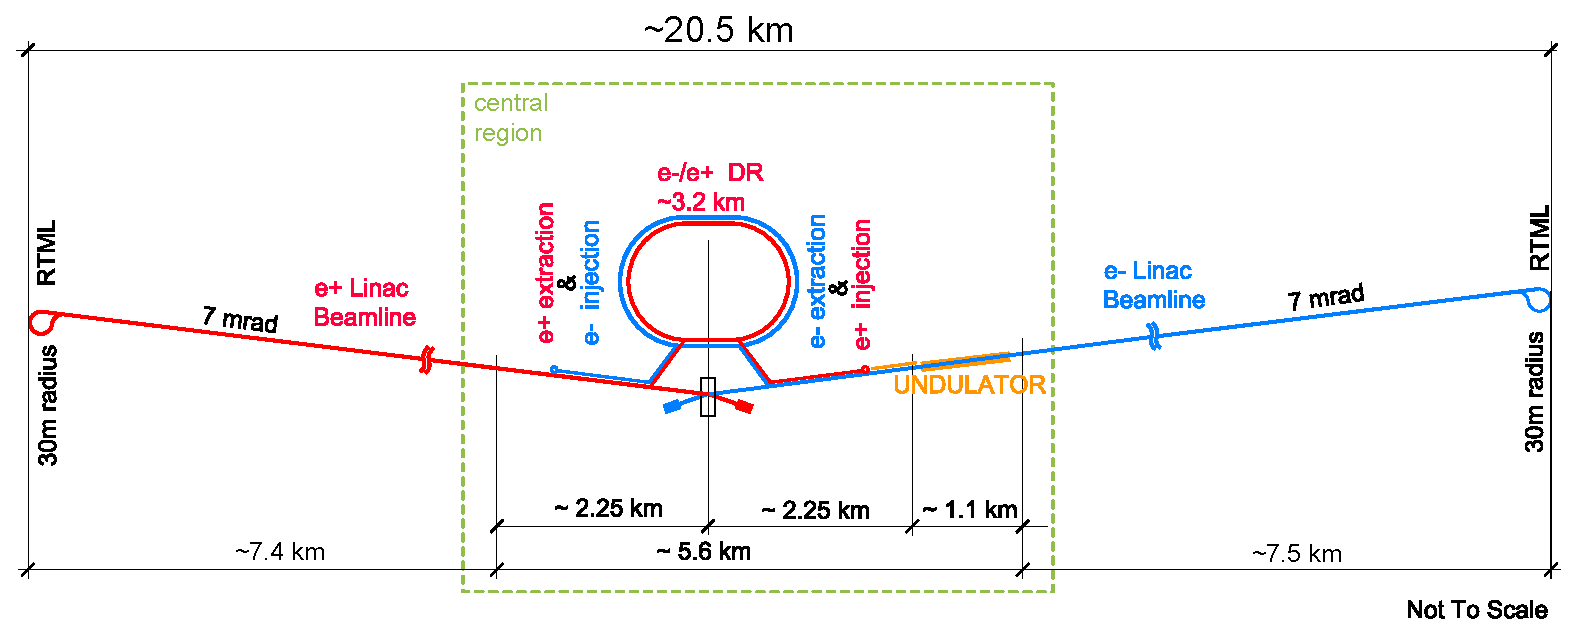
\includegraphics[width=\hsize]{chapters/figures/TDR-machine-layout-cartoon-staged-mirror.pdf}
\caption{Schematic layout of the ILC in the $250\,{\mathrm{GeV}}$ staged configuration.
\label{fig:ilc-schematic}}
 \end{center}
 \end{figure*}

\subsection{Design Evolution since the TDR}
\label{sec:design_evo}

Soon  after the discovery of the Higgs boson, the Technical Design Report (TDR) for the ILC accelerator was published in 2013~\cite{Adolphsen:2013jya,Adolphsen:2013kya} after 8 years of work by the Global Design Effort (GDE).
The TDR design was based on the requirements set forth by the ICFA mandated parameters committee~\cite{Heuer:2006}:
\begin{itemize}
\item a centre-of-mass energy of up to \siunit{500}{GeV},
\item tunability of the centre-of-mass energy between $\sqrt{s} = \siunit{200}{GeV}$
 and \siunit{500}{GeV},
\item  a luminosity sufficient to collect \siunit{500}{fb^{-1}} within four years of operation, taking into account three-year a ramp up, corresponding to a final luminosity of \siunit{250}{fb^{-1}} per year and an instantaneous luminosity of ${\mathcal{L}} = \siunit{2 \cdot 10^{34}}{cm^{-2}\,s^{-1}}$,
\item an electron polarisation of at least $80\,\%$,
\item  the option for a later upgrade to energies  up to \siunit{1}{TeV}.
\end{itemize}

The accelerator design presented in the TDR met these requirements (see Tab.~\ref{tab:ilc-params}), at an estimated construction cost of \siunit{7,982}{MILCU} for a Japanese site, plus \siunit{22.9}{Mh} (million hours) of labour in participating institutes~\cite[Sec. 15.8.4]{Adolphsen:2013kya}. 
Costs were expressed in ILC Currency Units ILCU, where \siunit{1}{ILCU} corresponds to \siunit{1}{US\$} at 2012 prices.

In the wake of the Higgs discovery, and the proposal by the Japan Association of High Energy Physicists (JAHEP) to host the ILC in Japan\cite{JAHEP:2012a} with its recommendation to start with a \siunit{250}{GeV} machine~\cite{JAHEP:2012b}, plans were made for a less expensive machine configuration with a centre--of--mass energy of $\sqrt{s} = \siunit{250}{GeV}$, around the maximum of the $Zh$ production cross section, half the TDR value.
Various options were studied in the TDR~\cite[Sect. 12.5]{Adolphsen:2013kya} and later~\cite{Dugan:2014}.
This resulted in a revised proposal~\cite{Evans:2017rvt} for an accelerator with an energy of \siunit{250}{GeV} and a luminosity of ${\mathcal{L}} = \siunit{1.35 \cdot 10^{34}}{cm^{-2}\,s^{-1}}$, capable of delivering about \siunit{400}{fb^{-1}} per year, or \siunit{200}{fb^{-1}} within the first four years of operation, taking into account the ramp-up.

Several other changes of the accelerator design have been approved by the ILC Change Management Board since 2013, in particular:
\begin{itemize}
\item The free space between the interaction point and the edge of the final focus quadrupoles ($L^*$) was unified between the ILD and SiD detectors~\cite{bib:cr-0002}, facilitating a machine layout with an optimised luminosity for both detectors. 
\item A vertical access shaft to the experimental cavern was foreseen~\cite{bib:cr-0003}, allowing a CMS-style assembly concept for the detectors, where large detector parts are built in an above-ground hall while the underground cavern is still being prepared. 
\item The shield wall thickness in the Main Linac tunnel was reduced from $3.5$ to \siunit{1.5}{m}~\cite{bib:cr-0012}, leading to a significant cost reduction. This was made possible by dropping the requirement for personnel access during beam operation of the main linac.
\item Power ratings for the main beam dumps, and intermediate beam dumps for beam aborts and machine tuning, were reduced to save costs~\cite{bib:cr-0013}.
\item A revision of the expected horizontal beam emittance at the interaction point at \siunit{125}{GeV} beam energy, based on improved performance expectations for the damping rings and a more thorough scrutiny of beam transport effects at lower beam energies, lead to an increase of the luminosity expectation from $0.82$ to \siunit{1.35 \cdot 10^{34}}{cm^{-2}\,s^{-1}}~\cite{bib:cr-0016}.
\end{itemize}

All these changes contributed to an overall cost reduction, risk reduction, and improved performance expectation.

Several possibilities were evaluated for the length of the initial tunnel. 
Options that include building tunnels with the length required for a machine with $\sqrt{s} = \siunit{350}{GeV}$ or \siunit{500}{GeV}, were considered.
In these scenarios, an energy upgrade would require the installation of additional cryomodules (with RF and cryogenic supplies), but little or no civil engineering activities.
In order to be as cost effective as possible, the final proposal, endorsed by ICFA~\cite{ICFA:2017}, does not include these empty tunnel options. 

While the length of the main linac tunnel was reduced, the beam delivery system and the main dumps are still designed to allow for an energy upgrade up to  $\sqrt{s} = \siunit{1}{TeV}$.


\subsection{Superconducting RF Technology}


%{\it Description of the TESLA SCRF technology - 4 pages
%
%Stresses long experience - FLASH, STF, XFEL, broad industrial base - LCLS-II, SHINE:
%addresses concerns mentioned in Nomura report and others (yield / gradient, MARX modulator)
%
%Nomura issue: MARX modulator
%
%Figures: Cavity, Cryomodule (Rey Hory) 
%
%}


The heart of the ILC accelerator are the two superconducting Main Linacs that accelerate both beams from \num{5} to \siunit{125}{GeV}.
These linacs are based on the TELAS technology:
beams are accelerated in \siunit{1.3}{GHz} nine-cell superconducting cavities made of niobium and operated at \siunit{2}{K} (Fig.~\ref{fig:tesla-cavity}). These 
 are assembled into cryo modules comprising eight to nine cavities, an optional quadrupole / corrector / beam position monitor unit, and all necessary cryogenic supply lines (Fig.~\ref{fig:crymodule}). 
Pulsed klystrons supply the necessary radio frequency power (High-Level RF HLRF) to the cavities by means of a waveguid power distribution system and input couplers, one per cavity.

This technology was primarily developed at DESY for the TESLA accelerator project that was proposed in 2001.
Since then, the TESLA technology collaboration~\cite{bib:ttc} has been improving this technology, which is now being used in several accelerators in operation (FLASH at DESY~\cite{schreiber_faatz_2015,Vogt:2018wvy}, European XFEL in Hamburg~\cite{bib:xfel}), under construction (LCLS-II at SLAC, Stanford, CA~\cite{bib:lcls-ii}) or planned (SHINE in Shanghai~\cite{Zhao:2018lcl}).


%\subsubsection{The Economics of Superconducting Linacs}
%
%The total energy dissipation $P\sub{d}$ in a linac cavity of length $L$ and a total voltage $V = g L$ at a the accelerating gradient $g$ is given by
%$$
%  P\sub{d} = g V R\sub{s} \lambda / C
%$$
%where $R\sub{s}$ is the material's surface resistance, $\lambda$ is the RF frequency, and $C$ (in ${\mathrm{\Omega^2}}$) depends only on the cavity shape, not its size.
%The dissipated power in a single cavity grows with the square of the gradient, 
%and the overall power grows linearly with the gradient for a given accelerating voltage.

\begin{figure*}[tbhp]
   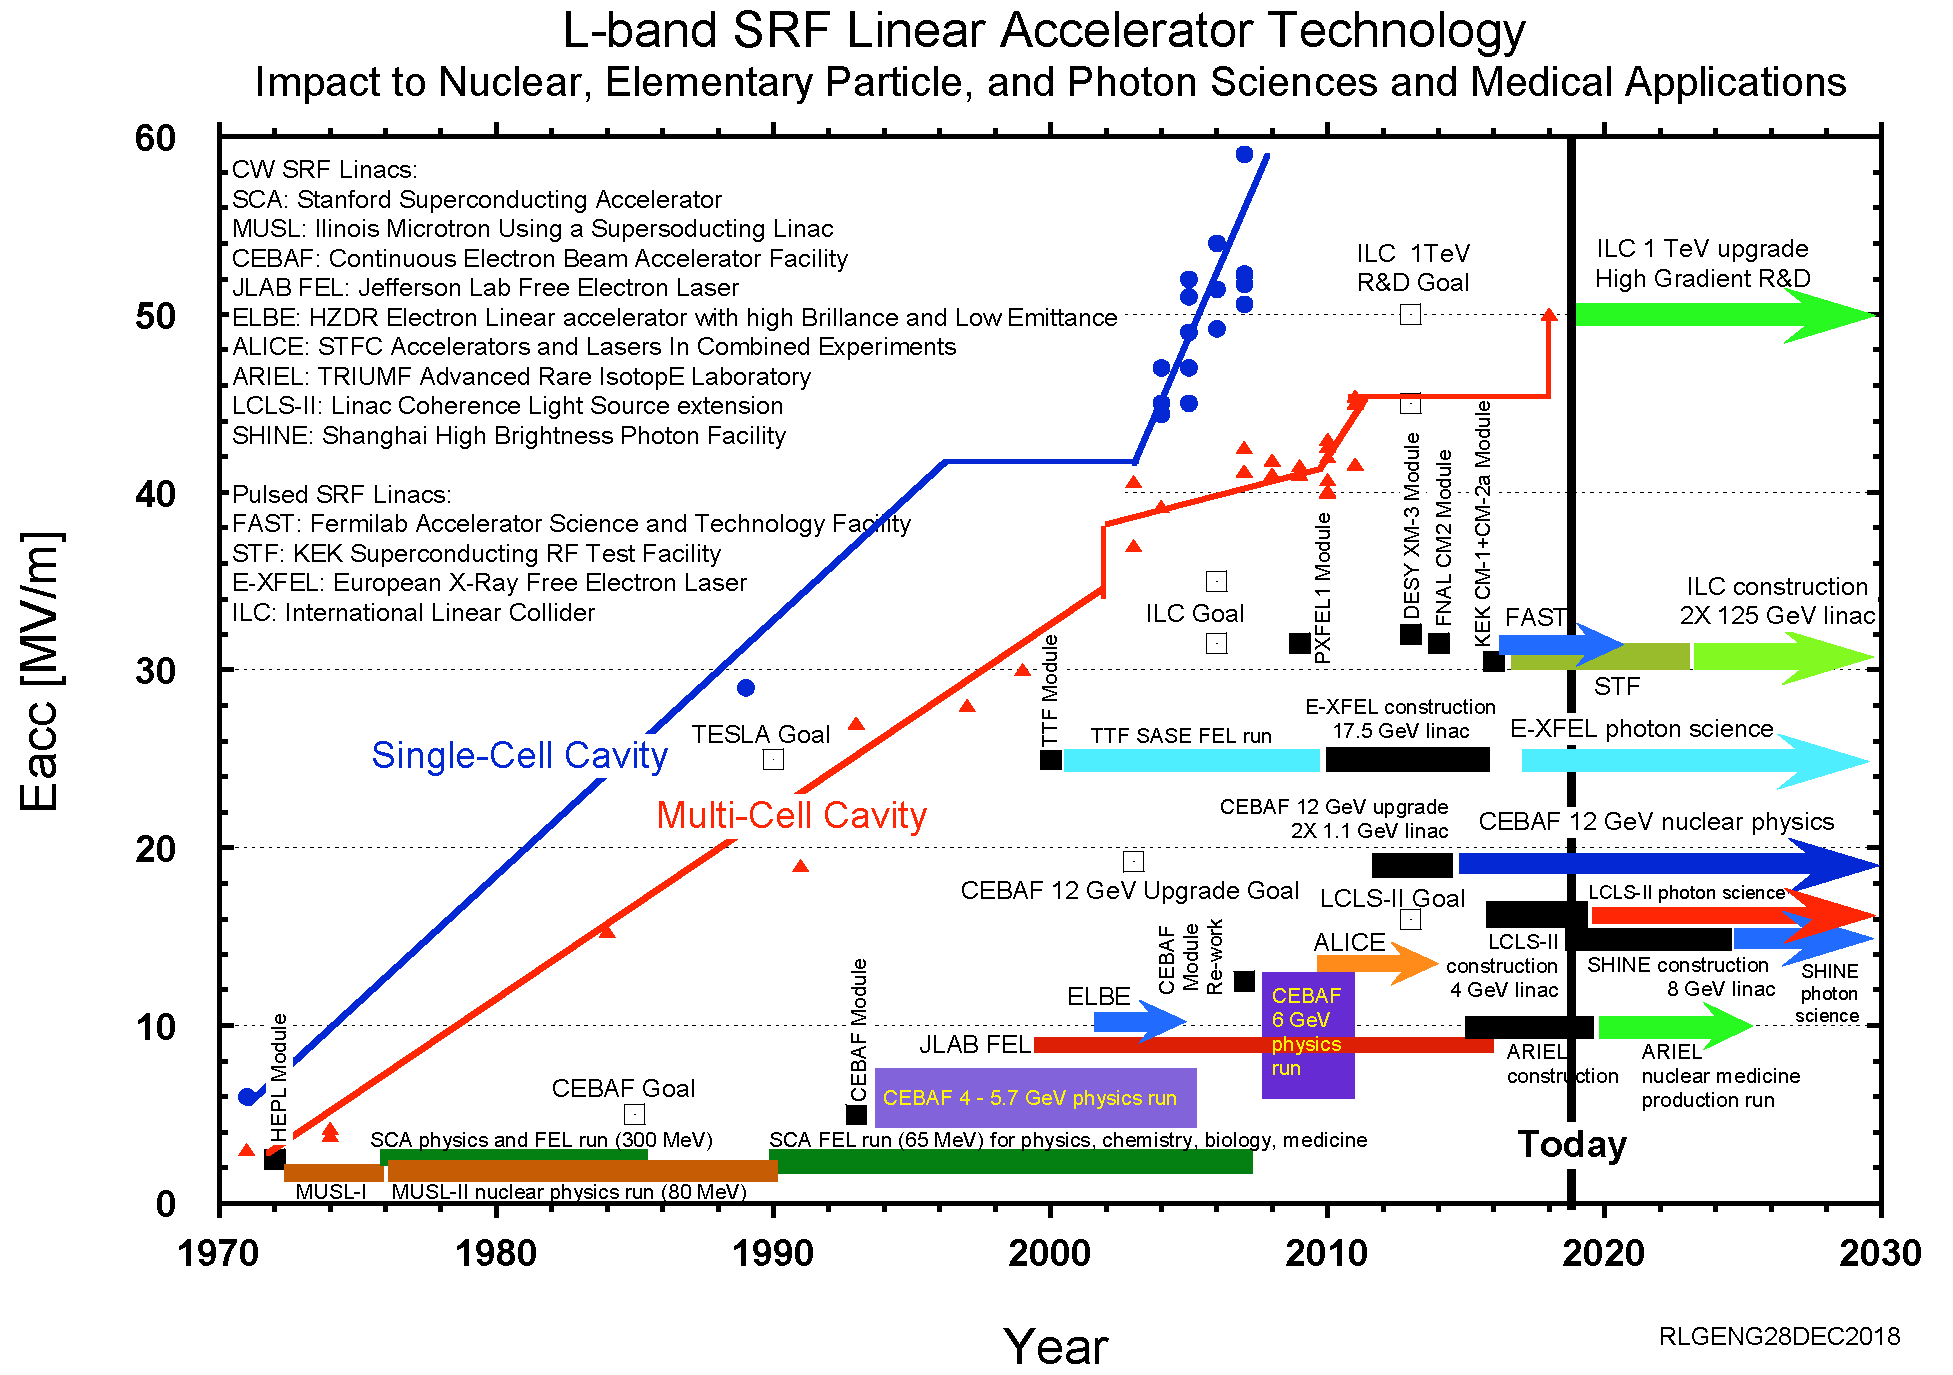
\includegraphics[width=0.8 \hsize]{chapters/figures/LBandSRFNbCavityGradientEvolution_ProjectImpact_rev28dec2018}
\caption{Development of the gradient of SRF cavities since 1970
\cite[updated]{Geng:2015glc}.
}
% Paper is published under CC-BY-3.0
\label{fig:gradients}
\end{figure*}

\subsubsection{The Quest for High Gradients}

The single most important parameter for the cost and performance of the ILC is the accelerating gradient $g$.
The TDR baseline value is an average gradient $g = \siunit{31.5}{MV/m}$ for beam operation, with a $\pm 20\,\%$ gradient spread between individual cavities.
Recent progress in R\&D for high gradient cavities raises the hope to raise the gradient by  $10\,\%$  to  $g = \siunit{35}{MV/m}$, which would reduce the total cost of the \siunit{250}{GeV} accelerator by about  $6\,\%$.
%% 6% = 50BY / 803BY
% Copied from TDR Vol 3.II p. 23
To achieve the desired gradient in beam operation, the gradient achieved in the low-power vertical test (mass production acceptance test) is specified $10\,\%$ higher to allow for operational gradient overhead for low-level
RF (LLRF) controls, as well as some degradation during cryomodule installation (few ${\mathrm{MV/m}}$).
Fig.~\ref{fig:gradients} shows how the achievable gradients have evolved over the past 50 years~\cite{Geng:2015glc}.

\paragraph{Gradient impact on costs:}
To the extent that the cost of cavities, cryomodules and tunnel infrastructure is independent of the achievable gradient, the investment cost per GeV of beam energy is inversely proportional to the average gradient achieved. This is the reason for the enormous cost saving potential from higher gradients.
This effect is partially offset by two factors:  the energy stored in the electromagnetic field of the cavity, and the dynamic heat load to the cavity from the electromagnetic field.  These grow quadratically with the gradient, and thus linearly for a given beam energy.
The electromagnetic energy stored in the cavity must be replenished by the RF source during the filling time that precedes the time when the RF is used to accelerate the beam passing through the cavity; this energy is lost after each pulse and thus reduces the overall efficiency and requires more or more powerful modulators and klystrons.
The overall cryogenic load is dominated by the dynamic heat load from the cavities, and thus operation at higher gradient requires larger cryogenic capacity.
Cost models that parametrise these effects indicate that the minimum of the investment cost per GeV beam energy lies at \num{50} or more GeV, depending on the relative costs of tunnel, SCRF infrastructure and cryo plants, and depending on the achievable $Q_0$~\cite{Adolphsen:2011a}. 
Thus,  the optimal gradient is significantly higher than the value of approximately \siunit{35}{MV/m} that is currently realistic; this emphasises  the relevance of achieving higher gradients.

It should be noted that in contrast to the initial investment, 
the operating costs rise when the gradient is increased, and this must be factored into 
the cost model.

\paragraph{Gradient limitations:}
Fundamentally, the achievable gradient of a SC cavity is limited by the point where the magnetic field at the cavity walls surpasses the critical field $H\sub{crit,RF}$ of the superconductor.
This gradient depends on the material, operating temperature, and the cavity geometry. 
For the TESLA type cavities employed at the ILC, this limit is about \siunit{48}{MV/m} at \siunit{2}{K}.
The best XFEL production cavity reached \siunit{44.6}{MV/m} (Fig.~\ref{fig:cavity-gradient}).
The record for single cell cavities operating at \siunit{1.3}{GHz} is \siunit{59}{MV/m}~\cite{Eremeev:2007zza}.
%
% Explanation:  
% 48MV/m using  $B\sub{pk}/g = \SIunit{4.26}{mT / (MV/m)}$ for ILC cavities~\cite{Adolphsen:2013kya}
% and the critical field for niobium at \SIunit{2}{K} has been measured to be \SIunit{205}{mT}~\cite{Padamsee:2009,Hays:1995zd}.
% , not far from the theoretical prediction of \SIunit{230}{mT}~\cite{Geng:2006wf}
% Padamsee:1998vf page 101 quotes 47MV/m for 4.2mT/MV/m
% Record 59MV/m corresponds to 206.5mT

Niobium is a type-II superconductor, and so it has two distinct superconducting phases, the Meissner state, with complete magnetic flux expulsion, which exists up to a field strength $H\sub{c1} \approx \siunit{180}{mT}/\mu_0$ ($\mu_0 = 4\pi \siunit{10^{-7}}{T\,m/A}$ being the vacuum permeability), and a mixed state in which flux vortices penetrate the material, up to a higher field strength $H\sub{c1}$, at which superconductivity breaks down completely.
In time-dependent fields, the penetrating vortices move due to the changing fields and thus dissipate energy, causing a thermal breakdown. 
However, for RF fields, the Meissner state may persis metastably up to the superheating field strength $H\sub{sh} \approx \siunit{240}{mT}/\mu_0$, which is expected to be the critical RF field critical field $H\sub{crit,RF}$~\cite{Padamsee:1998vf}.
Experimentally, niobium RF cavities have been operated at field strengths as high as $H=\siunit{206}{mT}/\mu_0$~\cite{Eremeev:2007zza}, and the best XFEL production cavities reach about $\siunit{190}{mT}$.
Recently, even \siunit{210}{mT} has been achieved at FNAL~\cite{Grassellino:2018tqg}.
In recent years, theoretical understanding of the nature of this metastable state and the mechanisms at the surface that prevent flux penetation has significantly improved~\cite{Gurevich:2017vnn,Kubo:2017cww}.
It appears that a thin layer of ``dirty'' niobium, \ie,  with interstitial impurities, on top of a clean bulk with good thermal conductivity, is favourable for high field operation.  

The gradient at which a SC cavity can be operated in practice is limited by three factors  factors in addition to those just listed~\cite{Padamsee:1998vf}:
\begin{itemize}
\item the thermal breakdown of superconductivity, when local power dissipation causes a local quench of the superconductor,
\item the decrease of the quality factor $Q_0$ at high gradients that leads to increased power dissipation,
\item the onset of field emission that causes the breakdown of the field in the cavity.
\end{itemize}
The onset of these adverse effects is mostly caused by micro-metre sized surface defects of various kinds. 
Producing a sufficiently defect-free surface in an economic way is thus the central challenge in cavity production.

More than 20 years of industrial production of TESLA type cavities have resulted in a good understanding which production steps steps and quality controls are necessary to produce cavities with high-quality, nearly defect-free surfaces that are capable of achieving the desired high field strengths at a reasonable production yield.


\paragraph{Results from XFEL cavity production:}

\begin{figure}[htbp]
   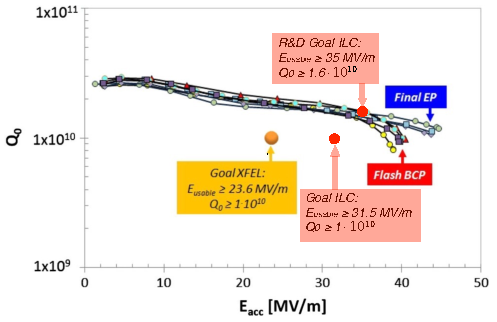
\includegraphics[width=\hsize]{chapters/figures/prab-19-092001-fig19-mod}
\caption{Examples of the $Q_0\,(E\sub{acc})$ curves of some of the best
cavities, either treated at RI using ``EP final'', or at EZ using
``BCP flash.''
\cite[Fig. 19]{Singer:2016fbf}. 
Vendor ``RI'' employs a production process that closely follows the ILC specifications, with a final electropolishing step.
The ILC gradient / $Q_0$ goals are overlaid.}
% Paper published under CC-BY-3.0
\label{fig:cavity-gradient}
\end{figure}

The production and testing of $831$ cavities for the European XFEL~\cite{Singer:2016fbf,Reschke:2017gjp} provides the biggest sample of cavity production data so far. 
Cavities were acquired from two different vendors RI and EZ,
of which vendor RI employed a production process with a final surface treatment closely following the ILC specifications, including a final electropolishing (EP) step,
while the second vendor EZ used buffered chemical polishing (BCP).
The XFEL specifications asked for a usable gradient of \siunit{23.6}{MV/m} with a $Q_0 \ge 1  \cdot 10^{10}$ for operation in the cryomodule;
with a $10\,\%$ margin this corresponds to a target value of \siunit{26}{MV/m} for the performance in the vertical test stand for single cavities.
Fig.~\ref{fig:cavity-gradient} shows the $Q_0$ data versus accelerating gradient of the best cavities received, with several cavities reaching more than \siunit{40}{MV/m}, significantly beyond the ILC goal, already with $Q_0$ values that approach the target value $1.6\cdot10^{10}$ that is the goal of future high-gradient R\&D.

\begin{figure}[htbp]
   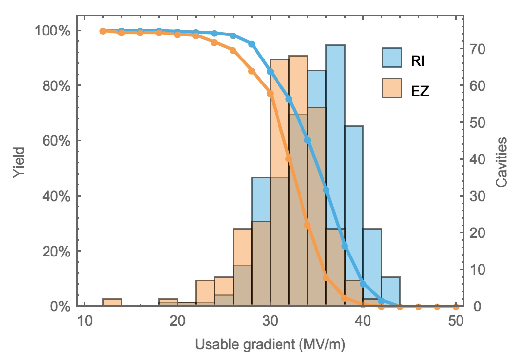
\includegraphics[width=\hsize]{chapters/figures/prab-20-042004-fig33}
\caption{Distribution and yield of the ``as received'' maximum
gradient of cavities produced for the European XFEL, separated by vendor \cite[Fig. 33]{Reschke:2017gjp}. 
Vendor ``RI'' employs a production process that closely follows the ILC specifications, with a final electro polishing step.}
% Paper published under CC-BY-4.0
\label{fig:cavity-yield}
\end{figure}


XFEL production data, in particular from vendor RI, provide excellent statistics for the cavity performance as received from the vendors, as shown in Fig.~\ref{fig:cavity-yield}.
For vendor ``RI'', the yield for cavities above \siunit{28}{MV/m} is $85\,\%$ of for the maximum gradient, with an average of \siunit{35.2}{MV/m}.

Since the XFEL performance goal was substantially lower than the ILC specifications, cavities with gradient below \siunit{28}{MV/m}, which would not meet ILC specifications, were not generally re-treated for higher gradients, limiting our knowledge of the effectiveness of re-treatment for large gradients.
Still, with some extrapolation it is possible to extract yield numbers applicable to the ILC specifications ~\cite{bib:Walker:2017.lcws}.

The XFEL data indicate that after re-treating cavities with gradients outside the ILC specification of $\siunit{35}{MV/m} \pm 20\,\%$, \ie, below \siunit{28}{MV/m}, a yield of $94\,\%$ for a maximum gradient above \siunit{28}{MV/m} can be achieved, with an average value of \siunit{35}{MV/m}, meeting the ILC specification.
Taking into account limitations from $Q_0$ and the onset of field emission, the usable gradient is lower.  Taking account of this gives a $82\,(91)\,\%$ yield and an average usable gradient of \siunit{33.4}{MV/m} after up to one (two) re-treatments.
The re-treatment and testing rate is significantly higher than assumed in the TDR, but the XFEL experience shows that re-treatment can mostly be limited to a simple high-pressure rinse (HPR) rather than an expensive electropolishing step.  

Overall, the XFEL cavity production data prove that it is possible to mass-produce cavities meeting the ILC specifications as laid out in the TDR with the required performance and yield.


\paragraph{High-gradient R\&D -- nitrogen infusion:}
\label{par:infusion}

\begin{figure}[htbp]
   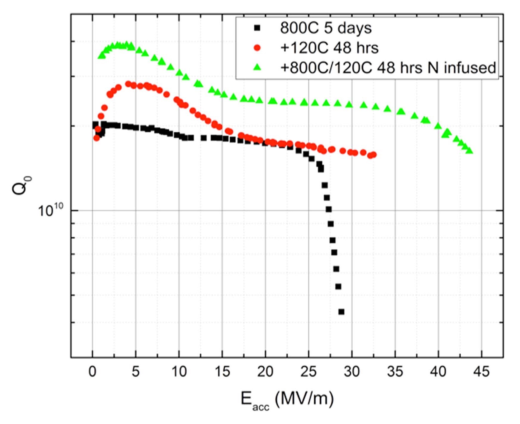
\includegraphics[width=\hsize]{chapters/figures/sst-30-094004-fig5}
\caption{Effect of successive cavity treatments on a single cavity: $\siunit{800}{^\circ C}$ bake for five days (black, lowest curve), followed by $48$ hours baking at $\siunit{120}{^\circ C}$ (red, middle curve). 
A third heat treatment including nitrogen infusion (green, top curve) significantly  raises the breakdown gradient and the quality factor of the cavity
\cite[Fig. 5]{Grassellino:2017bod}.
}
% Paper is published under CC-BY-3.0
\label{fig:n2infusion}
\end{figure}

In recent years, new techniques have emerged that seem to indicate that higher fields combined with higher quality factors are attainable in bulk niobium cavities.

In the early 2010s, nitrogen doping was developed as a method to substantially increase $Q_0$ by adding nitrogen during the \siunit{800}{^\circ C} baking, which leads to interstitial nitrogen close to the niobium surface~\cite{Grassellino:2013nza}.
This technique has been employed successfully in the production of the cavities for LCLS-II, with an average $Q_0$ of $3.0\cdot 10^{10}$ achieved in a prototype cryomodule~\cite{Wu:2018qyl}.
However, nitrogen doping reduces the critical RF field of the material and thus limits the achievable gradients to values below \siunit{30}{MV/m}, rendering doped material useless for high gradient applications.

By contrast, in nitrogen infusion the nitrogen is added during the low temperature baking at \siunit{120}{^\circ C}.
Experimental results seem to indicate that nitrogen infusion may offer a combination of three advantages:
\begin{itemize}
\item Reaching higher accelerating gradients,
\item higher $Q_0$ values, resulting in a reduced cryogenic load, 
\item a simplified and less expensive production process that does away with the final electropolishing step.
\end{itemize}

Fig.~\ref{fig:n2infusion} \cite[Fig. 5]{Grassellino:2017bod} shows how the addition of nitrogen during the final \siunit{48}{h} long \siunit{120}{^\circ C} bake of a one--cell cavity drastically improves the cavity quality factor as well as the maximum gradient, which comes close to the best XFEL cavity results, but at higher $Q_0$.

% XXX CONTINUE HERE XXX experimental status, success, transfer to other labs

Up to now, it has proven difficult to reproduce these exciting results in other laboratories.
Success has been reported by groups at JLAB~\cite{Dhakal:2017xxq}, and  Cornell~\cite{Koufalis:2017blg}, but KEK has reported mixed results \cite{bib:Umemori:2018.lcws}, and DESY has so far not been able to reproduce these results~\cite{Wenskat:2018zco}.
These difficulties seem to indicate that the recipe for a successful application of nitrogen infusion is not yet fully understood, and that further research and development will be necessary before this process can be transferred to industry. 

Nevertheless, the infusion results have triggered a renewed interest in the research on highest gradients in niobium cavities, with a host of new experimental results, increased activity to achieve a more thorough theoretical understanding~\cite{Kubo:2017cww,Gurevich:2017vnn}, and application of state-of-the-art analytical methods such as   muon spin rotation (muSR) \cite{Romanenko:2013saa}.
This provides reason for optimism that an improved understanding of the mechanisms that stabilise superconductivity in the presence of high fields will result in improved performance of industrially produced cavities for the ILC.

\paragraph{High-gradient R\&D -- alternative cavity shapes:}

Fundamentally, the achievable gradient in a niobium cavity is limited by the maximum magnetic field at the cavity surface, not the electrical field strengths.
The ratio between peak surface field $B\sub{pk}$ and gradient $g$ depends on the cavity geometry and is $B\sub{pk}/g = \siunit{4.26}{mT / (MV/m)}$ for TESLA type cavities.
A number of alternative cavity shapes have been investigated with lower ratios~\cite{Geng:2006wf},
resulting in single cells gradients up to \siunit{59}{MV/m}~\cite{Eremeev:2007zza}.
The reduced magnetic field, however, has to be balanced with other factors that favour the TESLA cavity shape, namely: a reasonable peak electrical field to limit the risk of field emission, sufficient iris width and cell-to--cell RF coupling, and a mechanical shape that can be efficiently fabricated.

Recently, new five-cell cavities with a new ``low surface field'' (LSF) shape~\cite{Li:2008a} have been produced at JLAB and have achieved gradient of up to~\siunit{50}{MV/m} in three of the five cells, which is a new record for multi-cell cavities~\cite{bib:Geng:2018.lcws}. 
The LSF shape aims to achieve a good compromise between the goal of a low magnetic field and the other criteria, and demonstrates that further improvements in gradient may be realised  in the future.


\subsubsection{Further Cost Reduction R\&D}

Additional strategies for cost reduction and improved cavity performance are also being investigated.

\paragraph{Low $RRR$ material:}

The niobium raw material and preparation of sheets  are a significant cost driver; R\&D is underway to re-evaluate the stringent limits on impurities, especially of tantalum, and the demand for a high residual resistivity ratio $RRR > 300$~\footnote{$RRR$ is the ratio of the material's room temperature resistivity to the normal conducting resistivity close to \siunit{0}{K}; heat conductivity from electrons is proportial to $RRR$. $RRR$ is reduced by impurities, in particular interstitial ones  from hydrogen, nitrogen and oxygen.}, to reduce the raw material cost.  The electrical 
conductivity and heat transport by electrons are proportional.  This implies that 
large $RRR$ values, indicative of low impurity content, make the cavities also 
less susceptible to thermal breakdown from surface defects.
However, when defect sizes can be successfully controlled to the extent necessary to achieve gradients above \siunit{35}{MV/m} routinely, the influence of heat conductivity and $RRR$ may be diminished, permitting the use of lower $RRR$ material~\cite{bib:Kubo:2018.ttc}.

\paragraph{Ingot and large-grain niobium:}

Together with direct slicing of discs from large niobium ingots, without rolling, forging and grinding or polishing steps, the cost for niobium sheets has the potential to be reduced by $50\,\%$~\cite{Evans:2017rvt,Kneisel:2014uqa}.
Without the mechanical deformation during rolling and forging, the grains from the initial crystallisation stay large, which makes later production steps, in particular deep--drawing of half cells, more challenging.
Nevertheless, if these challenges are overcome, tests with large--grain and ingot niobium show promising results~\cite{Reschke:2011a, Dhakal:2015xac}.


\subsubsection{Basic Parameters}

% Copied from TDR Vol 3.II p. 23
The choice of operating frequency is a balance between the higher cost of larger, lower-frequency cavities and the increased cost at higher frequency associated with the lower sustainable gradient from the increased surface resistivity. 
The optimum frequency is in the region of \siunit{1.5}{GHz}, but during the early R\&D on the technology, \siunit{1.3}{GHz} was chosen due to the commercial availability of high-power klystrons at that frequency.

\subsubsection{Cavities}

The superconducting accelerating cavities for the ILC are nine-cell structures made out of high-purity niobium (Fig.~\ref{fig:tesla-cavity}), with an overall length of \siunit{1.25}{m}.
Cavity production starts from niobium ingots which are forged and rolled into \siunit{2.8}{mm} thick niobium sheets that are individually checked for defects by an eddy current scan and optical inspection~\cite{Adolphsen:2013jya}.
Cavity cells are produced by deep-drawing the sheets into half cells, \num{18} of which are joined by electron beam welding with two end groups to form the whole structure.
This welding process is one of the most critical and cost-intensive steps of the cavity manufacturing procedure. 
Utmost care must be taken to avoid irregularities, impurities and inclusions in the weld itself, and deposition of molten material at the inner surface of the cavity that can lead to field emission.

\begin{figure}[htbp]
   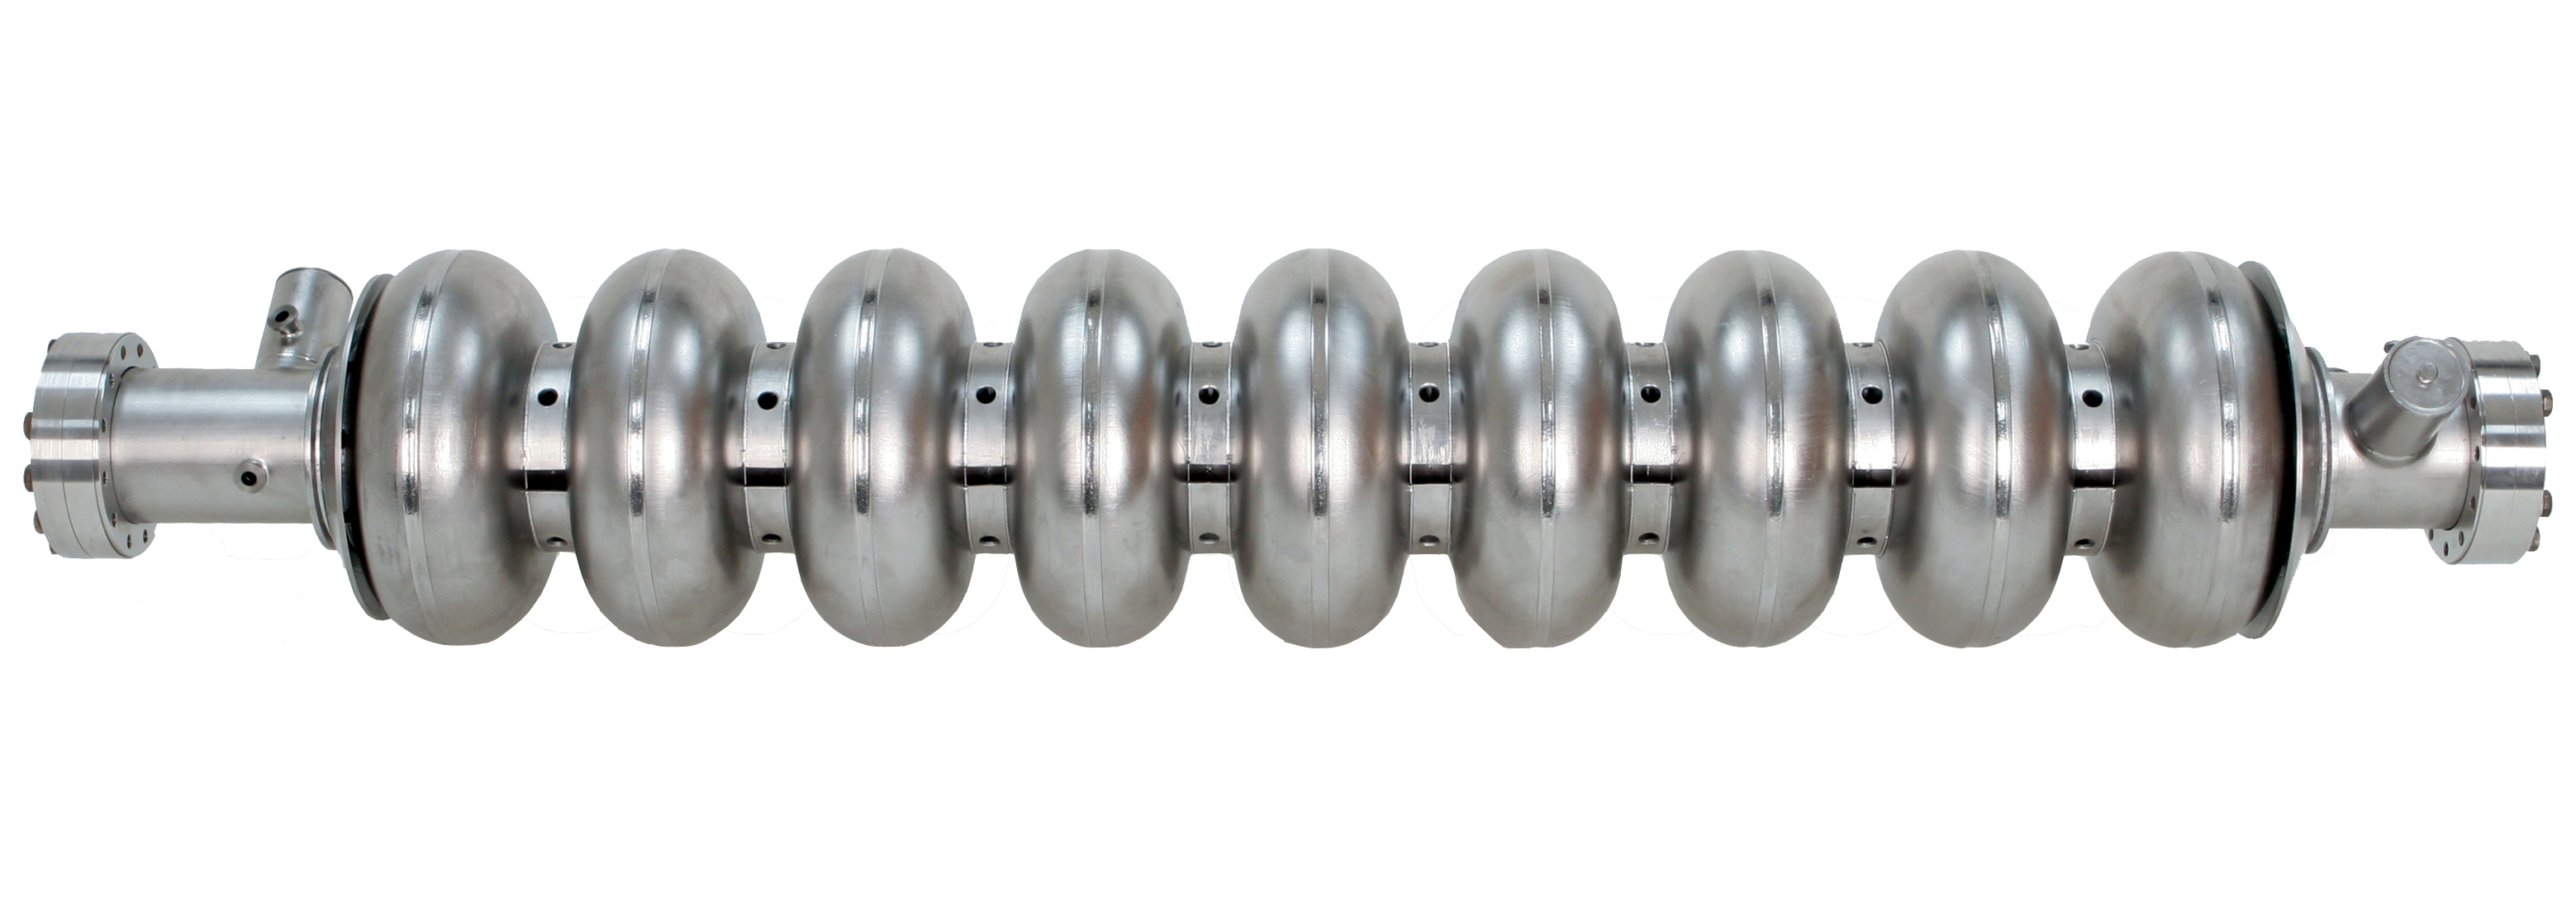
\includegraphics[width=\hsize]{chapters/figures/tesla9cell-cavity-2}
\caption{A $1.3\,{\mathrm{GHz}}$ superconducting niobium nine-cell cavity.
}
% Figure from TDR Executive Summary
% https://svnsrv.desy.de/k5websvn/wsvn/General.ilctdr/tags/FormOne-Print-Release/tdres/accel/figs/tesla9cell-cavity-2.jpg
\label{fig:tesla-cavity}
\end{figure}

After welding, the inner surface of the cavity must be prepared.
The process is designed to remove material damage incurred by chemical procedures during the fabrication process, remove chemical residues from earlier production steps, remove hydrogen in the bulk niobium from earlier chemical processing, and remove particulate contamination.
In a last step, the cavity is closed to form a hermetically sealed structure ready for transport.
The treatment steps involve a series of rinses with ethanol or high pressure water, annealing in a high purity vacuum furnace at \siunit{800^\circ}{C} and \siunit{120^\circ}{C}, and electro polishing or buffered chemical polishing.
The recipe for the surface preparation has been developed over a long time.  Still, it remains subject to optimisation, since it is a major cost driver for the cavity production and largely determines the overall performance and yield of the cavities.
In particular the electropolishing steps are complicated and costly, as they require complex infrastructure and highly toxic chemicals.
One advantage of nitrogen infusion (see Par.~\ref{par:infusion}) 
is that the final electropolishing step is omitted.

Careful quality control during the production process is of high importance.
At the European XFEL, several quality controls were conducted by the manufacturer during production, with nonconformities reported to the institute responsible for the procurement, where a decision was made whether to accept or reject a part~\cite{Singer:2016fbf}. 
With this ``build to print'' approach, in which the manufacturer guarantees that a precise production process will be followed but does not guarantee a specific performance, procurement costs are reduced, because the manufacturer does not carry, and does not charge for,  the performance risk.

Upon reception from the manufacturer, cavities are tested in a vertical cryostat (``vertical test''), where $Q_0$ is measured as a function of the gradient.
Cavities that fall below the specified gradient goal are re-treated by an additional (expensive) electropolishing step or a comparatively simple high--pressure rinse. 
After retreatment, the vertical test is repeated.

Re-treatment and tests constitute a major cost driver in cavity production. 
For the ILC TDR, it was assumed that $25\,\%$ of the cavities would fall below the \siunit{28}{MV/m} gradient threshold and undergo re-treatment and a second vertical test.
E-XFEL data from the vendor ``RI'' that followed the ILC production recipe indicate that $15\,\%$ to $37\,\%$ of the cavities fall below \siunit{28}{MV/m}, depending  on whether the maximum or the `usable'' achieved gradient is considered~\cite{bib:Walker:2017.lcws}.
However, E-XFEL experience also shows that, in most of the cases, a high-pressure rinse is sufficient as re-treatment to remove surface defects, which is a cost saving compared to the electropolishing assumed in the TDR.

After successful testing, prior to installation in the cryomodule, cavities are equipped with a magnetic shield and the frequency tuner, which exerts mechanical force on the cavity to adjust the resonant frequency to the frequency of the external RF field~\cite[Sect. 3.3]{Adolphsen:2013kya}.  


\subsubsection{Power Coupler}

The power coupler transfers the radio frequency (RF) power from the waveguide system to the cavity. 
In the ILC, a coupler with a variable coupling is employed; this is realised using  a movable antenna.  Another role of the coupler is to 
separate the cavity vacuum from the atmospheric pressure in the waveguide, and to  insulate the cavity at \siunit{2}{K} from the surrounding room temperature.
Thus,  the coupler has to fulfill a number of demanding requirements: transmission of high RF power with minimal losses and no sparking, vacuum tightness and robustness against window breaking, and minimal heat conductivity.  
As a consequence, the coupler design is highly complex, with a large number of components and several critical high-tech manufacturing steps.

The baseline coupler design was originally developed in the 1990s for the Tesla Test Facility (TTF, now FLASH) at DESY,
and has since been modified by a collaboration of LAL and DESY for use in the European XFEL.
$800$ of these couplers (depicted in Fig. \ref{fig:xfelcoupler}) were fabricated for the European XFEL~\cite{Kaabi:2013wna} by two different companies and are now in operation.
A lot of experience has been gained from this production~\cite{Sierra:2017wyc}.



\begin{figure}[htbp]
   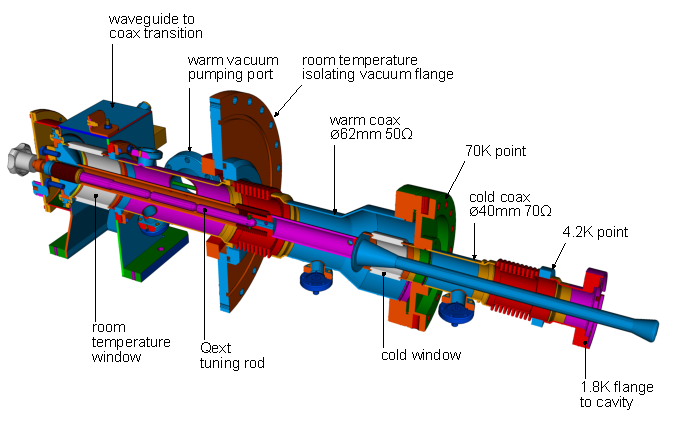
\includegraphics[width=\hsize]{chapters/figures/xfelcoupler}
\caption{An XFEL type coupler.
  % Fig from ILC TDR, should be OK to use
}
\label{fig:xfelcoupler}
\end{figure}


\subsubsection{Cryomodules}

\begin{figure}[htbp]
   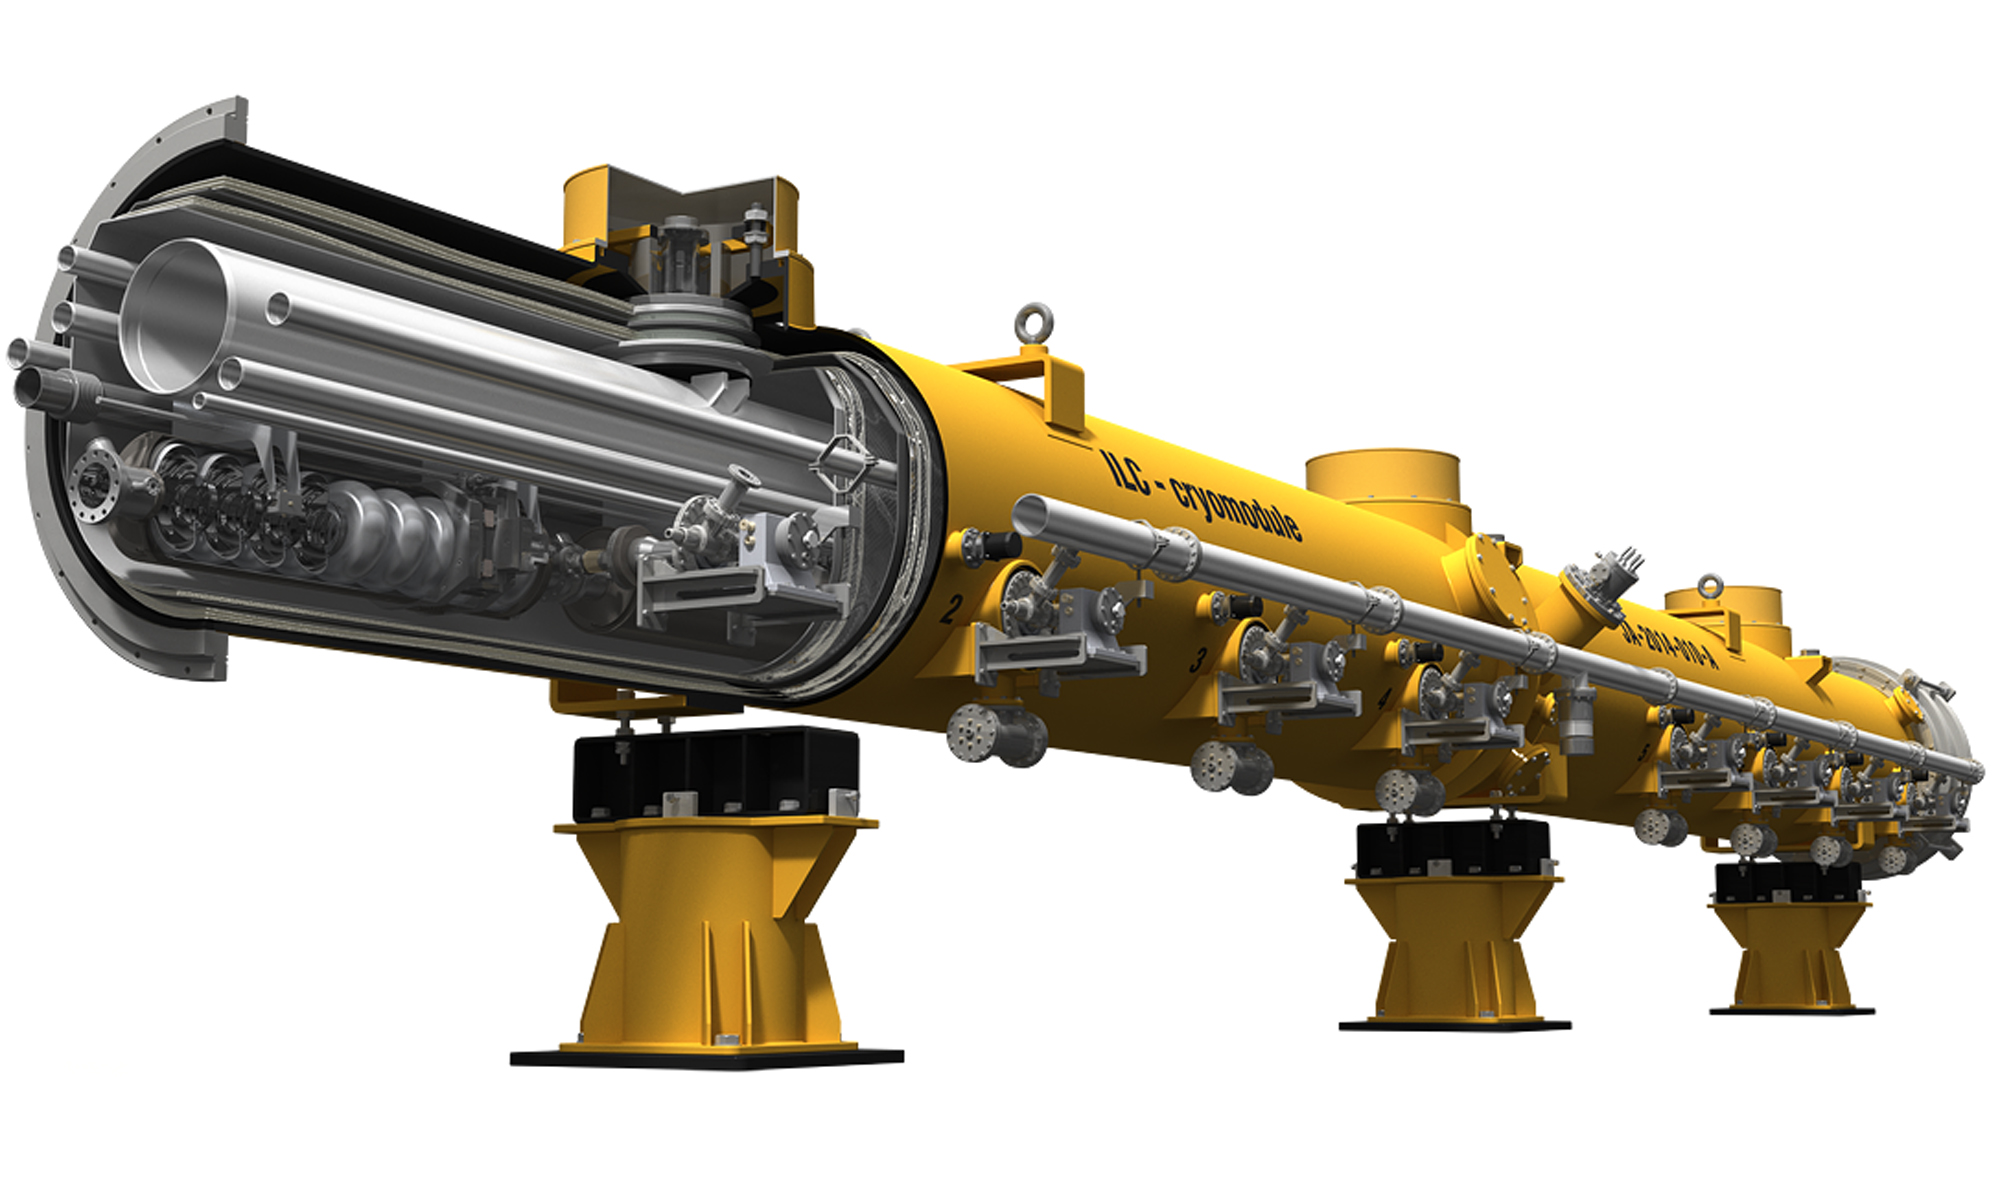
\includegraphics[width=\hsize]{chapters/figures/10_ILC_cryomodule}
\caption{An ILC type cryomodule. \copyright Rey.Hori/KEK.}
% Figure from Rey.Hori - check copyright!
% http://www.linearcollider.org/images/pid/1000890/gallery/10_ILC_cryomodule.jpg
\label{fig:crymodule}
\end{figure}

To facilitate transportation, installation and operation, 8 to 9 cavities are integrated into a \siunit{12.6}{m} long cryomodule~(Fig.~\ref{fig:crymodule}), which houses the cavities, thermal insulation, and all necessary supply tubes for liquid and gaseous helium at \siunit{2-80}{K} temperature.


\begin{figure}[htbp]
   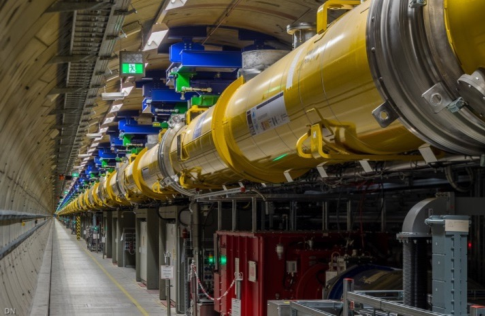
\includegraphics[width=\hsize]{chapters/figures/srf17-moxa02-fig1}
\caption{View of installed cryomodules in the tunnel of the European XFEL~\cite{Reschke:2018ywk}.
}
% Paper is published under CC-BY-3.0
\label{fig:xfel-tunnel}
\end{figure}


Nine of these cryomodules are connected in the tunnel to form a cryostring with a common liquid helium supply.  RF for one such string is provided by two klystrons.
No separate helium transfer line is necessary, as all helium transport lines are integrated within the modules.  A  quadrupole / beam position monitor / corrector magnet unit  is mounted instead of the 9th cavity in every third module.
Fig.~\ref{fig:xfel-tunnel} shows installed cryomodules in the tunnel of the European XFEL~\cite{Reschke:2018ywk}.

Cryomodule assembly requires a dedicated facility with large clean rooms, especially trained, experienced personnel, and thorough quality control~\cite{Berry:2017gpt}.
The cryomodules are certified for liquid helium pressure of up to \siunit{2}{bar}, which is why the have to conform to the applicable pressure vessel codes, which brings with it very stringent documentation requirements for all pressure bearing parts~\cite{Peterson:2011zz}.

For the European XFEL project, 101 cryomodules were assembled by industrial partners in a dedicated facility built and operated by CEA~\cite{Weise:2014zqa,Berry:2017gpt}, demonstrating the successful industrialization of the assembly process, with a final throughput of one cryomodule every four working days.
This production rate is close to the rate envisaged for a possible European contribution of 300 cryomodules to a \siunit{250}{GeV} ILC in Japan.

\begin{figure}[htbp]
   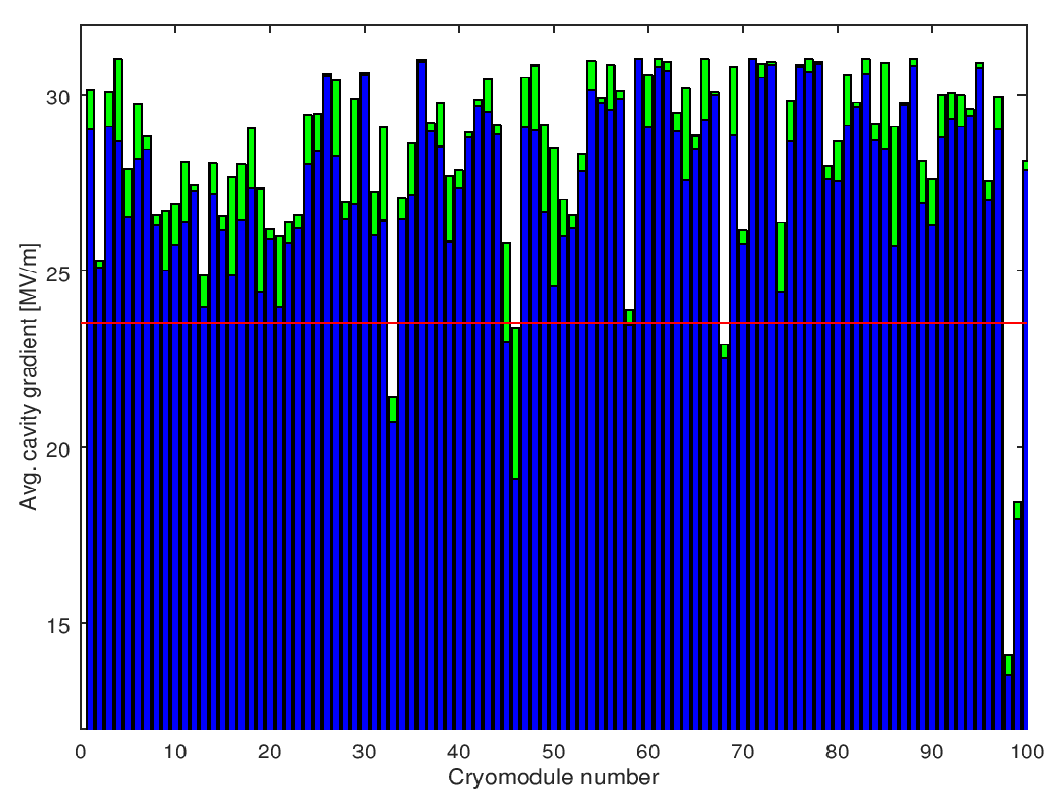
\includegraphics[width=\hsize]{chapters/figures/srf17-mopb106-fig1}
\caption{Average of the operating (blue) and maximum
(green) gradient for cavities in each European XFEL serial-production cryomodule.
The specification of \siunit{23.6}{MV/m} is marked by a red line
\cite{Kasprzak:2018kkr}.
}
% Paper is published under CC-BY-3.0
\label{fig:cryomodules-performance}
\end{figure}

While the design gradient for XFEL accelerator modules of \siunit{23.6}{MV/m} is significantly lower than the aim of \siunit{31.5-35}{MV/m} for the ILC, a number of cryomodules have been built around the world that come close or reach the ILC TDR specification of \siunit{31.5}{MV/m}: An XFEL prototype module at DESY was reached \siunit{30}{MV/m}~\cite{Kostin:2009a}, Fermilab has demonstrated cryomodule operation at the ILC specification of \siunit{31.5}{MV/m}~\cite{Broemmelsiek:2018iqr}, and KEK has reported stable pulsed operation of a cryomodule at \siunit{36}{MV/m}~\cite{Yamamoto:2018kml}.

Fig.~\ref{fig:cryomodules-performance} shows the average cavity gradients per cryomodule for the European XFEL serial-production cryomodules~\cite{Kasprzak:2018kkr}. 
For almost all of the modules, the cavity gradients are significantly above the XFEL specification of \siunit{23.6}{MV/m}.


\subsubsection{Plug-compatible design}

In order to allow various designs of sub-components from different countries and vendors to work together in the same cryomodule, a set of interface definitions has been internationally agreed upon.
This ``plug-compatible'' design ensures that components are interchangeable between modules from different regions and thus reduces the cost risk.
Corresponding interface definitions exist for the cavity, the fundamental-mode power coupler, the mechanical tuner and the helium tank.
The ``S1Global'' project~\cite{bib:s1g} has successfully built a single cryomodule from several cavities equipped with different couplers and tuners, demonstrating the viability of this concept.


\subsubsection{High-Level Radio-frequency}

The high-level radio-frequency (HLRF) system provides the RF power that drives the accelerating cavities.
The system comprises modulators, pulsed klystrons, and a waveguide power distribution system.


\paragraph{Modulators:}
The modulators provide the short, high-power electrical pulses required by the pulsed klystrons from a continuous supply of electricity. 
The ILC design foresees the use of novel, solid state Marx modulators.
These modulators are based on a solid-state switched capacitor network, where capacitors are charged in parallel over the long time between pulses, and discharged in series during the short pulse duration,
transforming continuous low-current, low voltage electricity into short high-power pulses of the required high voltage of \siunit{120}{kV} at a current of \siunit{140}{A}, over \siunit{1.65}{ms}.
Such Marx modulators have been developed at SLAC~\cite{Kemp:2011zz} 
and successfully tested at KEK~\cite{Gaudreau:2014pza}.
However, long-term data about the required large mean time between failures (MTFB) are not yet available.

\paragraph{Klystrons:}
The RF power to drive the accelerating cavities is provided by \siunit{10}{MW} L-band multi-beam klystrons. 
Devices meeting the ILC specifications were initially developed for the TESLA project, and later for the European XFEL.
They are now commercially available from two vendors (Thales and Toshiba), both of which provided klystrons for the E-XFEL.
The ILC specifications ask for a $65\,\%$ efficiency (drive beam to output RF power), which are met by the existing devices.

Recently, the High Efficiency International Klystron Activity (HEIKA) collaboration~\cite{Syratchev:2015a, Gerigk:2018ebm} has been formed that investigates novel techniques for high--efficiency klystrons.
Taking advantage of modern beam dynamic tools, methods such as the Bunching, Alignment and Collecting (BAC) method~\cite{Guzilov:2014a} and the Core Oscillation Method (COM)~\cite{Constable:2017hha} (Fig.~\ref{fig:com})
 have been developed that promise increased efficiencies up to $90\,\%$~\cite{Baikov:2015bif}.  
One advantage of these methods is that it is possible to increase the efficiency of existing klystrons by equipping them with a new electron optics, as was demonstrated retrofitting an existing tube from VDBT, Moscow. 
This increased the output power by almost 50\,\% and its efficiency from 42\,\% to 66\,\%~\cite{Jensen:2016a}.

To operate the ILC at an increased gradient of \siunit{35}{MV/m} would require that the maximum klystron output power is increased from $10$ to \siunit{11}{MW}. 
It is assumed that this will be possible by applying the results from this R\&D effort to high-efficiency klystrons.
 
\begin{figure}[htbp]
   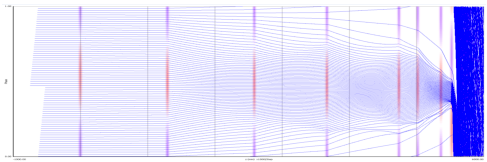
\includegraphics[width=\hsize]{chapters/figures/eefact16-wet3ah2-fig1}
\caption{Electron phase  profile of an \siunit{800}{MHz} klystron employing the Core Oscillation Method (COM)~\cite{Constable:2017hha}.
}
% Paper is published under CC-BY-3.0
\label{fig:com}
\end{figure}

\paragraph{Local Power--Distribution System (LPDS):}

In the baseline design, a single RF station with one modulator and klystron supplies RF to $39$ cavities, which corresponds to $4.5$ cryo--modules~\cite[Sec. 3.6.4]{Adolphsen:2013kya}. Then  $2$ klystrons drive a $9$ cryo--module cryo-string unit.
The power is distributed by the LPDS, a system of waveguides, power dividers and loads. 
All cavities from a $9$-cavity module and half of a $8$--cavity module are connected in one LPDS, and three such LPDS units are connected to one klystron.
This arrangement allows an easy refurbishment such that a third klystron can be added to a cryo-string, increasing the available power per cavity by $50\,\%$ for a luminosity upgrade (cf.\ Sec.~\ref{subsec:upg-opt}).

The LPDS design must provide a cost--effective solution for the  distribution of 
the RF power with minimal losses, and at the same time provide the 
flexibility to adjust the power delivered to each cavity by at least $\pm20\,\%$ to allow for 
the specified spread in maximum gradient. 
The LPDS design therefore contains remotely controlled, motor-driven Variable Power Dividers (VPD), phase shifters, and H--hybrids that can distribute the power with the required flexibility.
This design allows one to optimise the power distribution during operation, based on the cavity performance in the installed cryo--module, and thus to get the optimum performance out of the system.
It does not require a measurement of the individual cavity gradients after the module assembly, and is thus compatible with the ILC production scheme, where only a fraction of the cryo-modules are tested.
This is a notable difference from  the scheme employed at the European XFEL, where $100\,\%$ of the modules were tested, and the the power distribution for each module was tailored to the measured cavity gradients, saving investment costs for the LPDS but making the system less flexible.

\subsubsection{Cryogenics}

The operation of the large number of superconducting cryo--modules for the main linacs and the booster linacs of the sources requires a large--scale supply of liquid helium.
The cyo--modules operate at \siunit{2}{K} and are cooled with superfluid helium, which at \siunit{2}{K} has a vapour pressure of about \siunit{32}{mbar}.


The accelerator is supplied with liquid helium by several cryogenic plants~\cite[Sec. 3.5]{Adolphsen:2013kya} of a size similar to those in operation at CERN for the LHC, at Fermilab, and DESY,
with a cooling capacity equivalent to about \siunit{19}{kW} at \siunit{4.5}{K}.
The \siunit{2}{K} and \siunit{4.5}{K} helium refrigerators are located in an underground access hall~\cite{bib:cr-0014} that is connected to the surface, where the helium compressors, gas tanks and further cryogenic infrastructure are located.
The total helium inventory is approximately $310 000$ liquid litres or about $41$ metric tonnes, about one third of the LHC's helium inventory.  A factor 2 more helium is needed for 
500~GeV operation.


%\subsubsection{Existing and Future Facilities}

% XXXXX MORE HERE  XXXXXXXX

\subsubsection{Series Production and Industrialisation, Worldwide and in Europe}

Due to the construction of the European XFEL, the industrial basis for the key SCRF components is broad and mature, in particular in Europe.
Europe has a leading supplier for raw material. 
In all three regions (Europe, America, Asia), several vendors for cavities have been qualified for ILC type cavities, and provided cost estimates in the past.
Two leading cavity vendors are European companies that have profited from large scale production of cavities for XFEL; 
both have won contracts for LCLS-II as a consequence, which illustrates the potential to create revenue from outside Europe should the ILC be built.
RF couplers have also been successfully produced by European and  American vendors for the XFEL and LCLS-II projects.

ILC/TESLA type cryo modules have been built in laboratories around the world (DESY, CEA in Europe, FNAL and JLAB in America, KEK in Asia).
Series production has been established in America at Fermilab and JLAB for LCLS-II,.
The largest series production was conducted by CEA in France, again for the XFEL, with the assembly of \num{103} cryo modules in total by an industrial partner under the supervision of CEA personnel, with a final throughput of one cryo module produced every four working days.

ILC type, pulsed \siunit{10}{MW} klystrons are commercially available from two vendors in Japan and Europe.

For XFEL, China has been a supplier for niobium raw material and cryomodule cold masses (the cryostat with internal insulation and tubing).
For the planned SCLF project in Shanghai, China has started to develop cavity and cryo module production capabilities, which will further broaden the worldwide production capabilities for SCRF components.
This reduces the risk that prices are pushed up by a monopoly of manufacturers for a large scale order of components as required for the iLC.

Overall, European industry is well prepared to produce the high-tech, high-value SCRF components needed for the ILC, which would likely constitute largest fraction of any European in-kind contribution (IKC) to the ILC, at very competitive prices.
Thus, expenditure for the European IKC will likely stay in Europe, with an excellent chance to stay within the price range assumed in the value estimate.
Moreover, European companies are well poised to win additional contracts from other regions, increasing the economic benefit for Europe from an ILC project.



%===============================================================================

\subsection{Accelerator Design}

\subsubsection{Electron and Positron Sources}

The electron and positron sources are designed to produce \siunit{5}{GeV} beam pulses with a bunch charge that is $50\,\%$ higher than the design bunch charge of \siunit{3.2}{nC} ($\siunit{2\cdot 10^{10}}{e}$), in order to have sufficient reserve to compensate  any unforeseen inefficiencies in the beam transport.
In the baseline design, both sources produce polarized beams with the same time structure as the main beam, \ie, $1312$ bunches in a $\siunit{727}{\mu s}$ long pulse.

The electron source design~\cite{Adolphsen:2013kya} is based on the SLC polarized electron source, which has demonstarted that the bunch charge, polarisation and cathode lifetime parameters are feasible.
The long bunch trains of the ILC do require a newly developed laser system and powerful preaccelerator structures, for which preliminary designs are available.
The design calls for  a Ti:sapphire laser impinging on a photocathode based on a strained GaAs/GaAsP superlattice
structure, which will produce electron bunches with an expected polarisation of \siunit{85}{\%},
sufficient for \siunit{80}{\%} beam polarization at the interaction point, as demonstrated at SLAC~\cite{Alley:1995ia}.

The positron source poses a larger challenge. 

In the baseline design, hard gamma rays are produced in a helical undulator driven by the main electron beam, which are converted to positrons in a rotating target.
Positrons are captured in a flux concentrator or a quarter wave transformer, accelerated to \siunit{400}{MeV} in two normal conducting preaccelerators followed by a superconducting accelerator very similar to the main linac, before they are injected into the damping rings at \siunit{5}{GeV}.
Compared to planar undulators, the helical undulators produce twice as many photons, and with circular polarisation, which is transferred to the positrons produced in the target.
The positron polarisation thus achieved is $30\,\%$.
The E-166 experiment at SLAC has successfully demonstrated this concept  \cite{Alexander:2009nb}, albeit at intensities much lower than foreseen for the ILC. 
Technological challenges of the undulator source concept are the target heat load, the radiation load in the flux concentrator device, and the dumping of 
the high intensity photon beam remnant.

As an alternative, an electron-driven positron source concept has been developed.
In the electron-driven scheme, a \siunit{3}{GeV} electron beam from a dedicated normal conducting linac produces positrons in a rotating target.
The electron drive beam, being independent from the main linac, has a completely different time structure. 
Positrons are produced in $20$ pulses at \siunit{300}{Hz} with $66$ bunches each.  With this scheme, it takes about \siunit{67}{ms} to produce the  positrons needed for a single Main Linac pulse with its $1312$ bunches, compared to \siunit{0.8}{ms} for the undulator source.
This different time structure spreads the heat load on the target over a longer time, allowing a target rotation speed of only \siunit{5}{m/s} rather than \siunit{100}{m/s}, which reduces the engineering complexity of the target design, in particular the vacuum seals of the rotating parts.
Although not free from its own engineering challenges, such as the high beam loading in the normal conducting cavities, the electron driven design is currently considered to be a low risk design that is sure to work.

Aside from the low technical risk, the main advantage of the electron driven design is the independence of positron production and electron main linac operation, which is an advantage for accelerator commissioning and operation in general.
In particular, electron beam energies below \siunit{120}{GeV} for operation at the $Z$ resonance or the $WW$ threshold would be no problem.
The undulator source, on the other hand, offers the possibility to provide beams at the maximum repetition rate of \siunit{10}{Hz} given by the damping time in the damping rings of \siunit{100}{ms}, whereas the electron driven scheme is limited to \siunit{6}{Hz} due to the additional \siunit{66}{ms} for positron production.
The main difference between the concepts is the positron polarisation offered by the undulator source, which adds significantly to the physics capabilities of the machine.  The physics implications of positron polarization is discussed later in the report, in Secs.~\ref{subsec:beampol} and {subsec:polarisation}. 

Both concepts have been reviewed recently \cite{PWG:2018a} inside the ILC community, with the result that both source concepts appear viable, with no known show stoppers, but they
require some more engineering work. 
The decision on the choice will be taken once the project has been approved, based on the physics requirements, operational aspects, and technological maturity and risks. 

\paragraph{Beam polarisation and spin reversal}
\label{par:beampol}

At the ILC, the electron beam and potentially the positron beam are longitudinally polarised at the source, \ie,  the polarisation vector is oriented parallel or antiparallel 
to the beam direction.
Whenever a longitudinally polarised beam of energy $E\sub{beam}$ is deflected by an angle $\theta\sub{bend}$, the polarisation vector undergoes a BMT precession though through an angle $\theta\sub{pol} =  \gamma a \theta\sub{bend}$~\cite{Moffeit:2005pb}, 
with the Lorentz factor $\gamma = E\sub{beam}/m\sub{e}$ and the electron's anomalous magnetic moment $a = (g-2)/2$. 
To preserve the longitudinal beam polarisation during the long transport from the source through the damping rings to the start of the main linac, which involves many horizontal bends, the beam polarisation vector is rotated into the transverse plane, perpendicular to the damping ring plane, before the beam is transferred to the damping rings, and rotated back to a longitudinal direction by a set of spin rotators at the end of the RTML (see Sec.~\ref{sec:rtml}).
Through the use of two rotators, it is possible to bring the polarisation vector into any desired direction, and compensate any remaining net precession between these spin rotators and the interaction point, so that any desired longitudinal or transverse polarisation at the IP can be provided.

To control systematic effects, fast helicity reversal is required.  This is helicity reversal of each beam independently, on a pulse to pulse basis, which must be achieved without a change of the magnetic fields of the spin rotator magnets.
For the electron beam, a fast helicity reversal is possible through a flip of the cathode laser polarisation.  For the undulator-based positron source, the photon polarisation is given by the undulator field.  Two parallel sets of spin rotators in front of the damping rings are used that rotate the polarisation vector either to the $+y$ or $-y$ direction.  With this scheme,
fast kickers can select a path through either of the two spin rotators and thus provide a fast spin reversal capability~\cite{Moffeit:2005pb,Malysheva:2016jdr}.




\subsubsection{Damping Rings}

The ILC includes two oval damping rings of \siunit{3.2}{km} circumference, sharing a common tunnel in the central accelerator complex.
The damping rings reduce the horizontal and vertical emittance of the beams by almost six orders of magnitude\footnote{The vertical emittance of the positrons is reduced from $\epsilon_{\mathrm{y}} \approx 0.8\,{\mathrm{\mu m}}$ to $2\,{\mathrm{pm}}$.} within a time span of only \siunit{100}{ms}, to provide the low emittance beams required at the interaction point. 
Both damping rings operate at an energy of \siunit{5}{GeV}.

The damping rings' main objectives are
\begin{itemize} 
\item to accept electron and positron beams at large emittance and produce the low-emittance beams required for high-luminosity production,
\item to dampen the incoming beam jitter to provide highly stable beams,
\item to 
delay bunches from the source to allow feed-forward systems to compensate for pulse-to-pulse variations in parameters such as the bunch charge.
\end{itemize}

Compared to today's fourth generation light sources, the target value for the normalized beam emittance ($\siunit{4}{\mu m}$/\siunit{20}{nm} for the normalised horizontal / vertical beam emittance) is low, but not a record value, and it is thus considered to be a realistic goal.

The main challenges for the damping ring design are to provide
\begin{itemize} 
\item a sufficient dynamic aperture to cope with the large injected emittance of the positrons,
\item a low equilibrium emittance in the horizontal plane,
\item a very low emittance in the vertical plane,
\item a small damping time constant,
\item damping of instabilities from electron clouds (for the positron DR) and fast ions (for the electron DR),
\item a small (\siunit{3.2-6.4}{ns}) bunch spacing, requiring very fast kickers for injection and ejection.
\end{itemize}

Careful optimization has resulted in a TME (Theoretical Minimum Emittance) style lattice for the arcs that balances a low horizontal emittance with the required large dynamic aperture~\cite[Chap. 6]{Adolphsen:2013kya}. 
Recently, the horizontal emittance has been reduced further by lowering the dispersion in the arcs through the use of longer dipoles~\cite{bib:cr-0016}.
The emittance in the vertical plane is minimised by careful alignment of the magnets and tuning of the closed orbit to compensate for misalignments and field errors, as demonstrated at the CESRTA accelerator~\cite{Billing:2011zc}.

The required small damping time constant requires large synchrotron radiation damping, which is provided by the insertion of $54$ wigglers in each ring.
This results in an energy loss of up to $7.7\,{\mathrm{MV}}$ per turn and up to $3.3\,{\mathrm{MW}}$ RF power to 
store the positron beam at the design current of $390\,{\mathrm{mA}}$.  This
actually exceeds the average beam power of the accelerated positron beam, $2.6\,{\mathrm{MW}}$ at 
a $250\,{\mathrm{GeV}}$.

Electron cloud (EC) and fast ion (FI) instabilities limit the overall current in the damping rings to about \siunit{400-800}{mA}, where the EC limit that affects the positrons is assumed to be more stringent. 
These instabilities arise from electrons and ions being attracted by the circulating beam towards the beam axis. 
A low base vacuum pressure of \siunit{10^{-7}}{Pa} is required to limit these effects to the required level.
In addition, gaps between bunch trains of around $50$ bunches are required in the DR filling pattern, which permits the use of clearing electrodes to mitigate EC formation.
These techniques have been developed and tested at the CESR-TA facility~\cite{Conway:2012zza}

In the damping rings, the bunch separation is only \siunit{6.4}{ns} (\siunit{3.2}{ns} for a luminosity upgrade to $2625$ bunches). 
Extracting individual bunches without affecting their emittance requires kickers with rise/fall times of \siunit{3}{ns} or less.
Such systems have been tested at ATF~\cite{Naito:2010zzb}.

The damping ring RF system will employ superconducting cavities operating at half the Main Linac frequency (\siunit{650}{MHz}).
Klystrons and accelerator modules can be scaled from existing \siunit{500}{MHz} units in operation at CESR and KEK~\cite[Sec. 6.6]{Adolphsen:2013kya}. 


\subsubsection{Low Emittance Beam Transport: Ring to Main Linac (RTML)}
\label{sec:rtml}

The Ring to Main Linac (RTML) system~\cite[Chap. 7]{Adolphsen:2013kya} is responsible for transporting and matching the beam from the Damping Ring to the entrance of the Main Linac.
Its main objectives are
\begin{itemize} 
\item transport of the beams from the Damping Rings at the center of the accelerator complex to the upstream ends of the Main Linacs,
\item collimation of the beam halo generated in the Damping Rings,
\item rotation of the spin polarisation vector from the vertical to the desired angle at the IP (typically, in longitudinal direction).
\end{itemize}

The RTML consists of two arms for the positrons and the electrons. 
Each arm comprises a damping ring extraction line transferring the beams from the damping ring extraction into the main linac tunnel, a long low emittance transfer line (LTL), the turnaround section at the upstream end of each accelerator arm, and a spin rotation and diagnostics section.

The long transport line is the largest, most costly part of the RTML.
The main challenge is to transport the low emittance beam at \siunit{5}{GeV} with minimal emittance increase, and in a cost-effective manner, considering that its total length is about \siunit{14}{km} for the \siunit{250}{GeV} machine.

In order to preserve the polarisation of the particles generated in the sources, their spins are rotated into a vertical direction (perpendicular to the Damping Ring plane) before injection into the Damping Rings. 
A set of two rotators~\cite{Emma:1995kf} employing superconducting solenoids allows to rotate the spin into any direction required.

At the end of the RTML, after the spin rotation section and before injection into the bunch compressors (which are considered part of the Main Linac, not the RTML~\cite{bib:cr-0010}), a diagnostics section allows measurement of  the emittance and the  coupling between the  horizontal and vertical plane.
A skew quadrupole system is included to correct for any such coupling.

A number of circular fixed-aperture and rectangular variable-aperture collimators in the RTML provide betatron collimation at the beginning of the LTL, in the turn around and before the bunch compressors.


\subsubsection{Bunch Compressors and Main Linac}

\begin{figure}[htbp]
   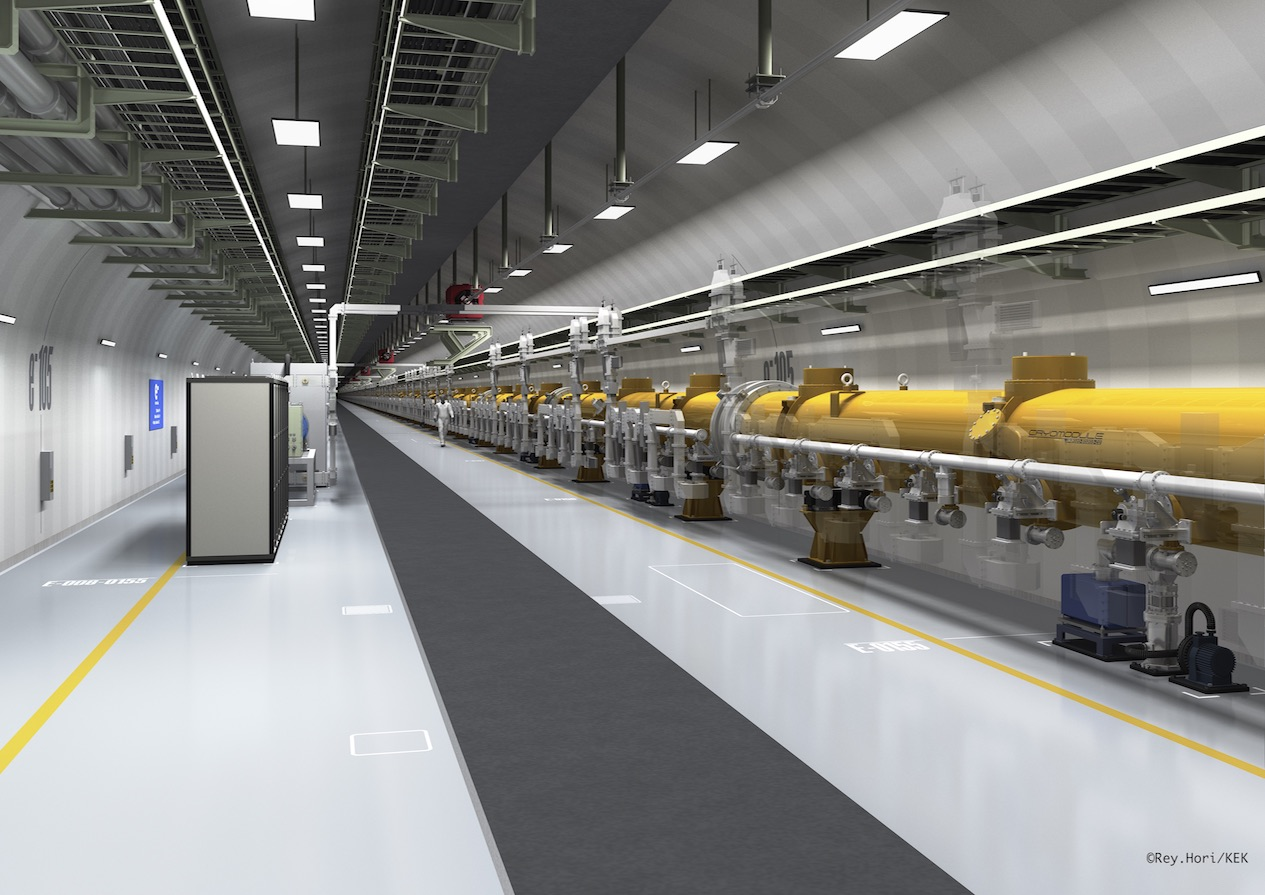
\includegraphics[width=\hsize]{chapters/figures/ILC2016_tunnel_A1_160826-low4}
\caption{Artist's rendition of the ILC Main Linac tunnel. The shield wall in the middle has been removed.
\copyright Rey.Hori/KEK.}
\label{fig:ilc-tunnel}
\end{figure}

The heart of the ILC are the two Main Linacs, which accelerate the beams from $5$ to \siunit{125}{GeV}.
The linac tunnel, as depicted in Figs.~\ref{fig:ilc-tunnel} and \ref{fig:ml-tunnel}, has two parts, separated by a shield wall. 
One side (on the right in Fig.~\ref{fig:ilc-tunnel}) houses the beamline with the accelerating cryomodules as well as the RTML beamline hanging on the ceiling.
The other side contains power supplies, control electronics, and the modulators and klystrons of the High-Level RF system.
The concrete shield wall (indicated as a dark-grey strip in in Fig.~\ref{fig:ilc-tunnel}) has a thickness of \siunit{1.5}{m}~\cite{bib:cr-0012}.
The shield wall allows access to the electronics, klystrons and modulators during operation of the klystrons with cold, resonant cavities, protecting personnel from X-ray radiation emanating from the cavities caused by dark currents.
Access during beam operation, which would require a wall thickness of \siunit{3.5}{m}, is not possible.

\begin{figure}[htbp]
   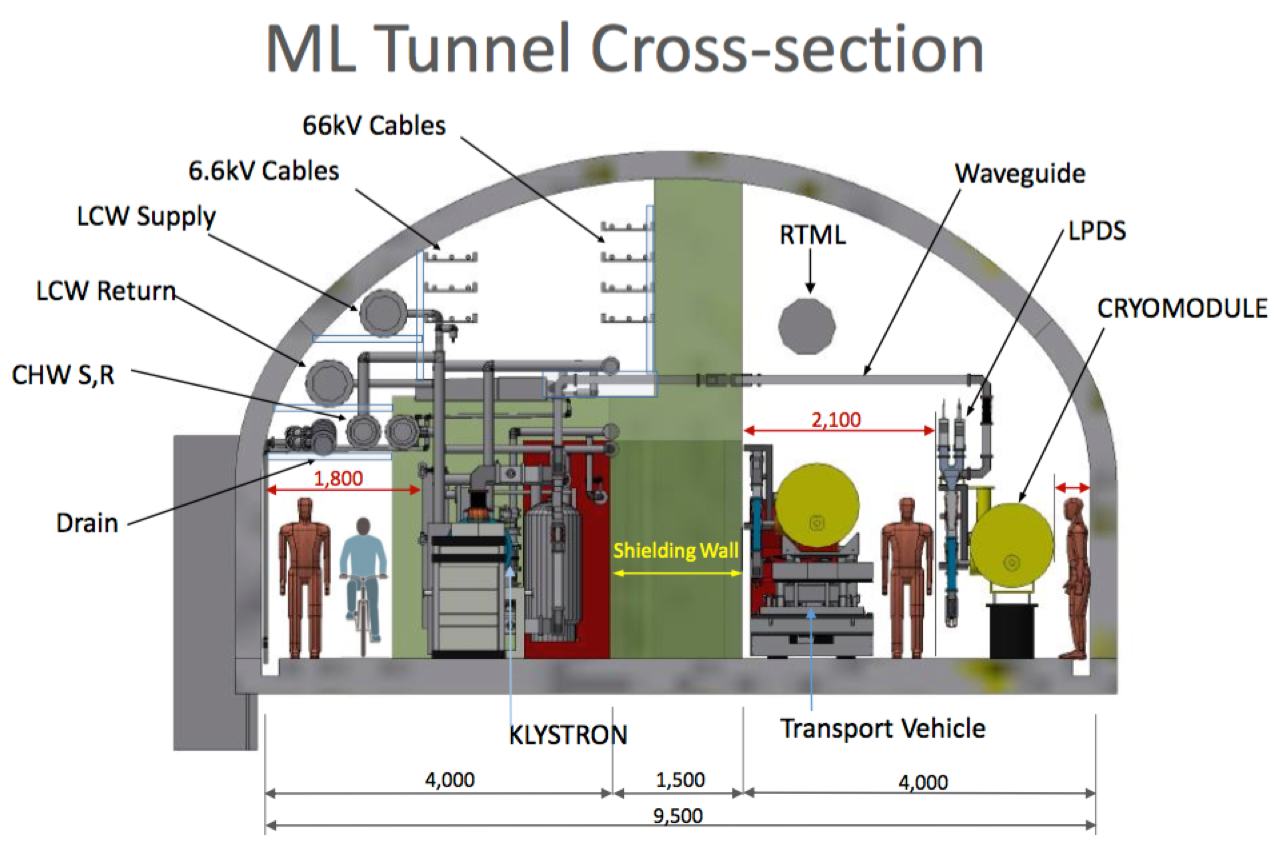
\includegraphics[width=\hsize]{chapters/figures/ML-cross-section}
\caption{Cross section through the Main Linac tunnel.}
\label{fig:ml-tunnel}
\end{figure}

The first part of the Main Linac is a two-stage bunch compressor system~\cite[Sec. 7.3.3.5]{Adolphsen:2013kya}, each consisting of an accelerating section followed by a wiggler. 
The first stage operates at \siunit{5}{GeV}, with no net acceleration, the second stage accelerates the beam to \siunit{15}{GeV}.
The bunch compressors reduce the bunch length from $6$ to \siunit{0.3}{mm}.

After the bunch compressors, the Main Linac continues for about \siunit{6}{km} with four long strings of cryomodules. 

\paragraph{RF distribution:}

Each \siunit{12.65}{m} long cryomodule contains $9$ cavities, or for every third module, $8$ cavities and a package with a superconducting quadrupole, corrector magnets, and beam position monitor.
Nine such modules, with a total of $117$ cavities, are powered by $2$ klystrons and provide 3.83 (4.29)~\GeV at a gradient of \siunit{31.5 (35)}{MV/m}.
The waveguide distribution system allows an easy refurbishment to connect a third klystron for a luminosity upgrade.
The $50\,\%$ RF power increase would allow $50\,\%$ higher current through smaller bunch separation, and longer beam pulses because of a reduced filling time, so that the number of bunches per pulse and hence the luminosity can be doubled, while the RF pulse duration of \siunit{1.65}{ms} stays constant.

\paragraph{Cryogenic supply:}


Each $9$ module unit \siunit{114}{m} long, forms a cryo string, which is connected to the helium supply line with a Joule-Thomson valve.
All helium lines are part of the cryomodule, obliterating the need for a separate helium transfer line. 
Up to $21$ strings with $189$ modules and \siunit{2.4}{km} total length can be connected to a single plant; 
this is limited by practical plant sizes and the gas--return header pressure drop.  


\paragraph{Cost reduction from larger gradients:}

Fig.~\ref{fig:ml-cryo-opta} shows the layout of the cryogenic supply system for the \siunit{250}{GeV} machine.
At the top, the situation is depicted for the gradient of \siunit{31.5}{MV/m} with a quality factor of $Q\sub{0}=1.0\cdot 10^{10}$, as assumed in the TDR~\cite{Adolphsen:2013kya}. 
In this case, the access points PM$\pm 10$ would house two cryogenic plants, each supplying up to $189$ cryomodules or an equivalent cryogenic load.
The bottom picture shows the situation for a gradient of \siunit{35}{MV/m} with $Q\sub{0}=1.6\cdot 10^{10}$, as could be expected from successful R\&D. 
The increased gradient would  allow reduction of the total number of cryomodules by roughly $10\,\%$ from $987$ to $906$. The increased quality factor would reduce the dynamic losses such that $4$ cryo plants would provide sufficient helium. In the top configuration $6$ large plants in the access halls plus $2$ smaller plants in the central region would be needed.

In all of these ways, the accelerator is designed to make good use of any anticipated performance gain from continued high gradient R\&D,  in the case that raising the gradient is
seen to be  beneficial from an economical point of view, without incurring unwanted technology risk.

\begin{figure}[htbp]
   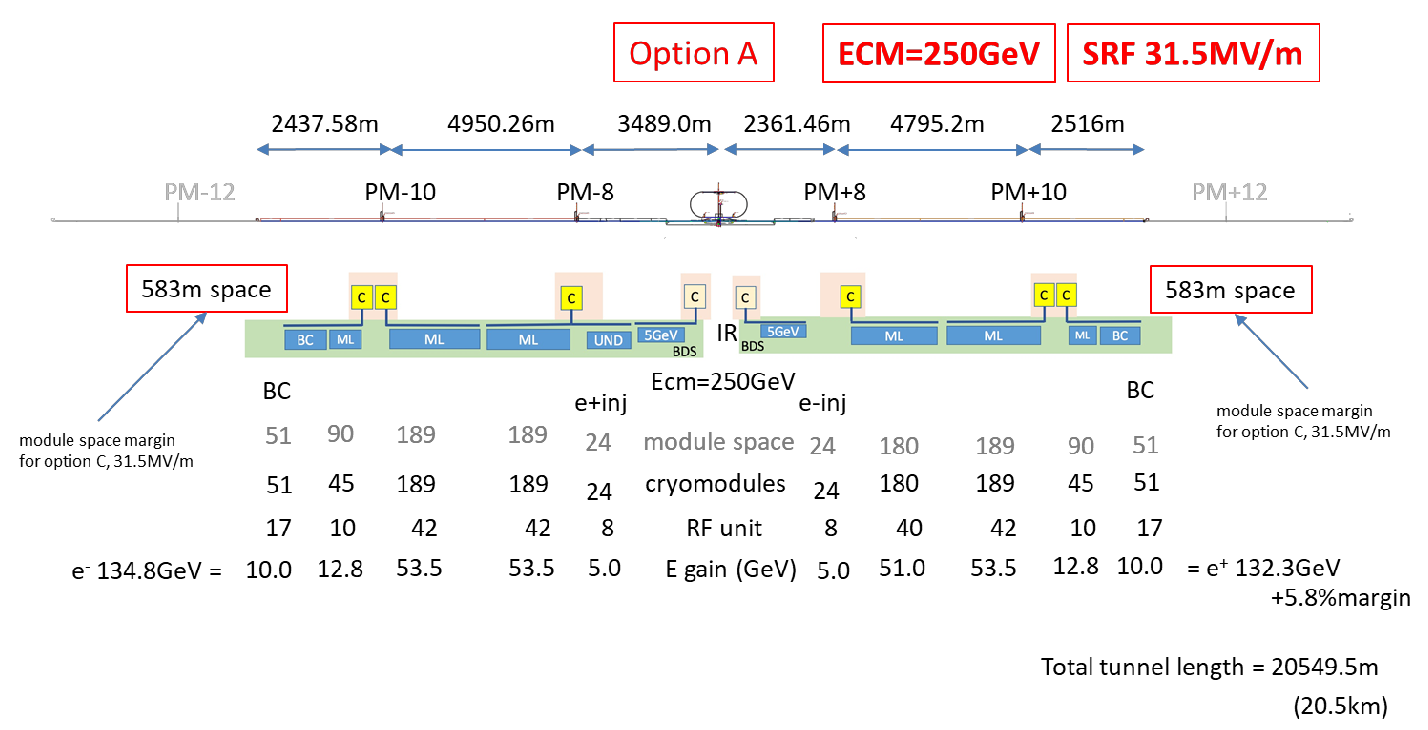
\includegraphics[width=\hsize]{chapters/figures/arxiv-1711-00568-fig-3-4}
   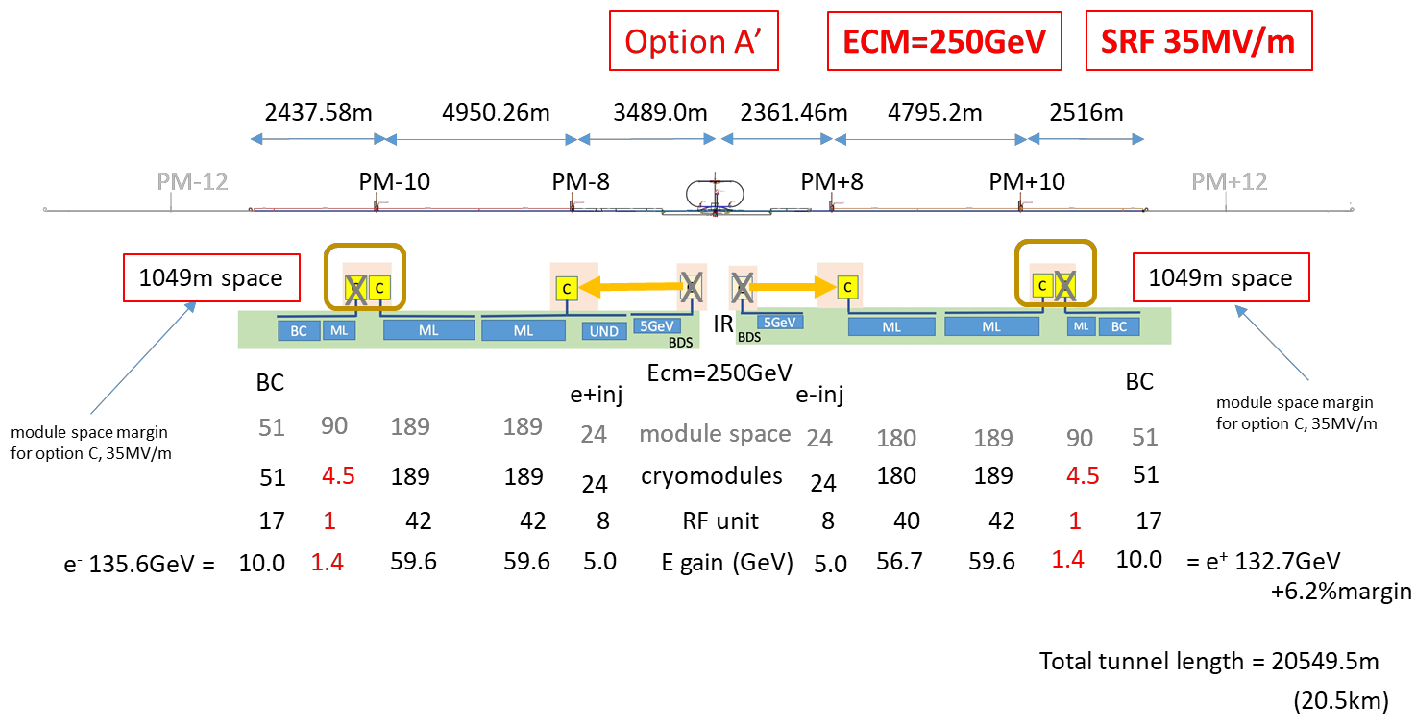
\includegraphics[width=\hsize]{chapters/figures/arxiv-1711-00568-fig-3-7}
\caption{Cryogenic layout for a gradient of \siunit{31.5}{MV/m} (top) and \siunit{35}{MV/m} (bottom)~\cite{Evans:2017rvt}.
``Module space'' indicates how many cryomodules can be physically installed, ``cryomodules'' and ``RF unit'' indicates the number of actually installed modules and klystrons (one klystron per 4.5 cryomodules). ``E gain'' indicates the energy gain in GeV. ``BC'', ``ML'', ``e+ inj'', ``e- inj'' and ``UND'' refer to the sections with need for liquid helium: bunch compressor, main linac, 5GeV boosters in the positron and electron source, and the positron source undulator section, respectively. PM$\pm8, 10, 12$ refer to access hall locations, ``C'' to cryo plants; meter numbers on top indicate the length of the corresponding section.}
\label{fig:ml-cryo-opta}
\end{figure}



\subsubsection{Beam Delivery System and Machine Detector Interface}

The Beam Delivery System (BDS) transports the $e^+/e^-$ beams from the end of the main linacs, focuses them to the required small beam spot at the Interaction Point (IP), brings them into collision, and transports the spent beams to the main dumps~\cite[Chap. 8]{Adolphsen:2013kya}.
The main functions of the BDS are
\begin{itemize}
\item measuring the main linac beam and matching it into the final focus,
\item protecting beamline and detector from mis-steered beams~\footnote{On the electron side, the protective fast beam abort system is actually located upstream of the positron source undulator.},
\item remove large amplitude (beam--halo) and off--momentum particles from the beam to minimize background in the detector,
\item accurately measure the key parameters energy and polarisation before and after the collisions.
\end{itemize}
The BDS must provide sufficient diagnostic and feedback systems to achieve these goals.

The BDS is designed such that it can be upgraded to a maximum beam energy of \siunit{500}{GeV}; components such as the dumps that are not cost drivers for the overall project but would be cumbersome to replace later are dimensioned for the maximum beam energy from the beginning.
In other places, such as the energy collimation dogleg, those components necessary for \siunit{125}{GeV} beam operation are installed and space for a later upgrade is reserved.

Overall, the BDS is \siunit{2254}{m} long from the end of the main linac (or the undulator and target bypass insert of the positron source on the electron side, respectively) to the IP.

\paragraph{Diagnostics and collimation section:}
The BDS starts with a diagnostics section, where emittance, energy and polarisation are measured and any coupling between the vertical and horizontal planes is corrected by a set of skew quadrupoles.
The energy measurement is incorporated into the machine protection system and can, \eg,  extract off-momentum bunches caused by a klystron failure in the main linac that would otherwise damage the machine or detector.
An emergency dump~\cite{bib:cr-0013} is dimensioned such that it can absorb a full beam pulse at \siunit{500}{GeV}, sufficient for \siunit{1}{TeV} operation.

The diagnostics section is followed by a collimation system, which first removes beam halo particles (betatron collimation). 
Then, off-momentum particles are removed.
In this energy collimation section, sufficient dispersion must be generated by bending the beam in a dogleg, while avoiding excessive synchrotron radiation generation in dispersive regions that leads to an increase of the horizontal emittance.
This emittance dilution effect grows as $E\sub{beam}^6$ at constant bending radius for the normalised emittance, and determines the overall length of the energy collimation section for a maximum \siunit{500}{GeV} beam energy to about \siunit{400}{m}.


\paragraph {Final focus with feedback system and crab cavities:}

The final focus system demagnifies the beam to the required spot size of \siunit{516 \times 7.7}{nm^2} by means of a final quadrupole doublet.
Even the relatively small energy spread of $\approx 0.1\,\%$ leads to a significant spread of the focal length of the doublet and requires a correction to achieve the desired beam size, which is realised by a local chromaticity correction scheme~\cite{Raimondi:2000cx}.

To bring the beams to collision with the neccessary nanometre accuracy requires a continuous compensation of drift and vibration effects.
Along the ILC, the pulse length and bunch separation (\siunit{727}{\mu s} and \siunit{554}{ns}, respectively) are large enough to allow corrections between pulses as well as within a bunch train (intratrain feedback).
Beam-beam offsets of a fraction of the beam size lead to a measurable deflection of the outgoing beams,and these measurements are used to feed fast stripline kickers that stabilize the beam.
\siunit{3.9}{GHz} crab cavities close to the interaction point are incorporated that rotate the bunches to compensate for the \siunit{14}{mrad} beam crossing angle~\cite[Sect. 8.9]{Adolphsen:2013kya}.
 

\paragraph {Test results from ATF2:}
The Accelerator Test Facility 2 (ATF2) was built at KEK in 2008 as a test bed for the ILC final focus scheme~\cite[Sec. 3.6]{Adolphsen:2013jya}.
Its primary goals were~\cite{Grishanov:2005ek,Grishanov:2006kx} to achieve a \siunit{37}{nm} vertical beam size at the interaction point (IP), and to demonstrate beam stabilisation at the nanometre level.
After scaling for the different beam energies (ATF2 operates at $E\sub{beam}=\siunit{1.3}{GeV}$), the \siunit{37}{nm} beam size corresponds to the TDR design value of $\sigma\sub{y}^* = \siunit{5.7}{nm}$ at \siunit{250}{GeV} beam energy.
As Fig.~\ref{fig:atf-results} shows, this goal has been reached within $10\,\%$~\cite{Okugi:2017jji} by the successive application of various correction and stabilisation techniques, 
validating the final focus design, in particular the local chromaticity correction~\cite{White:2014vwa}.

The fifth generation FONT5 feedback system~\cite{Apsimon:2018bpq} for the ILC and CLIC has also been tested at the ATF2, where a beam stabilisation to \siunit{41}{nm} has been demonstrated~\cite{Ramjiawan:2018egu}.

\begin{figure}[htbp]
   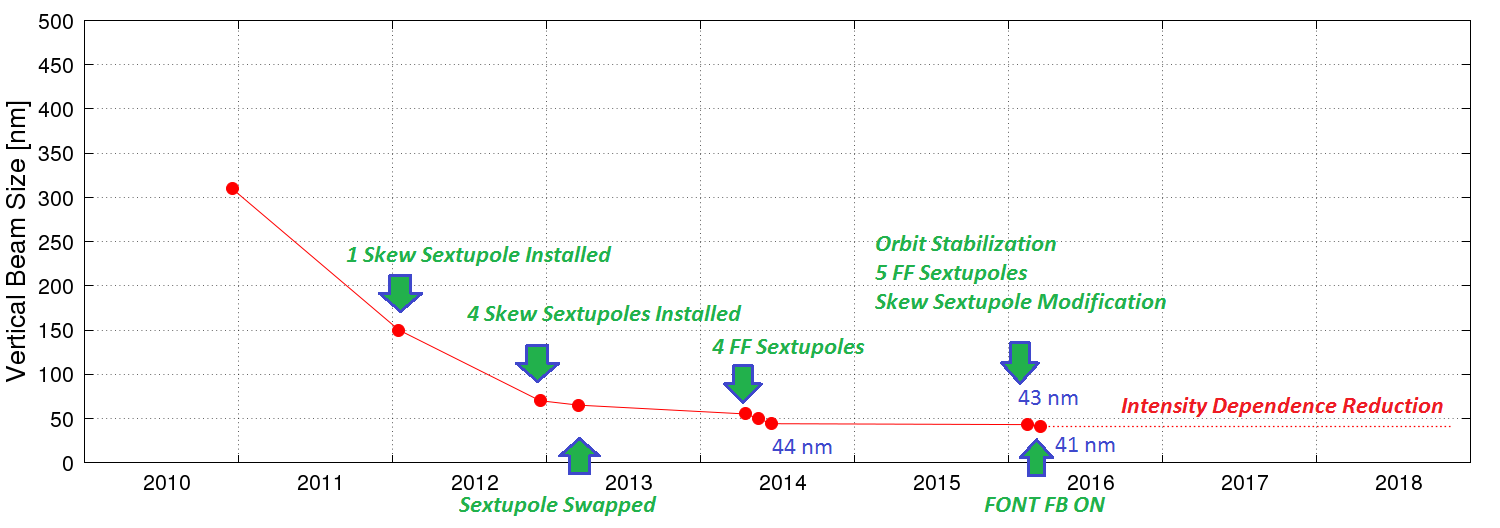
\includegraphics[width=\hsize]{chapters/figures/ATF2trend2018}
\caption{Beamsizes achieved at the Accelerator Test Facility 2 (ATF2) as a function of time~\cite{bib:atf2esu}. The latest result (\siunit{41}{nm}~\cite{Okugi:2017jji}) is within $10\,\%$ of the goal beam size of \siunit{37}{nm}.}
\label{fig:atf-results}
\end{figure}

\paragraph {Machine detector interface (MDI):}

% describe experimental hall, final focus

% XXXXXXXXXXXXX CONTINUE HERE XXXXXXXXXXXXXX


\paragraph {Extraction line:}

% XXXXXXXXXXXXX CONTINUE HERE XXXXXXXXXXXXXX


\paragraph {Main dump:}

The main beam dumps~\cite[Sect. 8.8]{Adolphsen:2013kya} are rated for a maximum beam power of \siunit{17}{MW}~\cite{bib:cr-0013}, enough for a \siunit{1}{TeV} upgrade of the accelerator.
The main dump design is based on the successful SLAC \siunit{2.2}{MW} beam dump~\cite{Walz:1967nz}.
It  utilises water at \siunit{10}{bar} pressure (to prevent boiling) as absorber medium. 
The main engineering challenges lie in the safe recombination of the produced oxyhydrogen gas and in the safe containment and disposal of radioisotopes, in particular tritium and $^7{\mathrm{Be}}$ produced from spallation processes.
The entry window is another component that has to be carefully designed. 


%===============================================================================

\subsection{Upgrade Options \label{subsec:upg-opt}}

Given the high initial investment for a facility as large as the ILC, it is mandatory to have an interesting physics programme for several decades, with the possibility to adapt the programme to the needs arising from the knowledge obtained by the LHC, the ILC itself, all other particle physics experiments, and other branches of physics such as cosmology.
Several options exist for upgrades of the ILC in terms of energy, luminosity, and beam polarisation.

\subsubsection{Energy upgrade}
\label{subsubsec:upg-optE}

The obvious advantage of a linear collider is its upgradeability in energy.
Basically, the main linacs can be extended as far as desired, at constant cost per added beam energy, with some added cost for the relocation of the turn arounds and bunch compressors.
Additional costs arise when the beam delivery system (BDS), including the beam dumps, has to be extended to handle the increased beam anergy; 
the current ILC BDS is designed to be easily upgradeable for centre of mass energies up to \siunit{1}{TeV} at minimal cost.

Depending on the actual gradient achieved for the construction of the ILC, there may be space for the installation of up to $171$ additional cryomodules, which would increase the centre-of-mass energy by about \siunit{54}{GeV} to around \siunit{304}{GeV}, as Fig.~\ref{fig:ml-cryo-opta} shows, 
and possibly require the installation of two additional cryo plants.

A further energy upgrade would require extension of the tunnel.
The Kitakami site can accommodate a total accelerator length of at least \siunit{50}{km}, more than enough for a \siunit{1}{TeV} centre--of--mass energy.
Any extension of the accelerator would proceed by adding new cryomodules at the low energy (upstream) ends of the accelerator, there is no need to move modules already installed. 

An upgrade would likely proceed in two phases: a preparation phase while the accelerator is still operated and produces data, and a refurbishment phase where the accelerator is shut down.

During the preparation phase, the necessary components---in particular the cryomodules, klystrons, and modulators---would be acquired and built.
At the same time, civil engineering would proceed with the excavation of new access tunnels, underground halls, and the main tunnel.
Recent studies conducted during road tunnel construction in the Kitakami area, in the same rock formation as foreseen for the ILC, indicate that the level of vibrations caused by tunnelling activities would allow to bring the new tunnels quite close to the existing ones before machine operation would be affected~\cite{bib:sanuki:lcws2018}, minimising the shutdown time necessary.

During the installation phase, the newly built tunnels would be connected to the existing ones, the beam lines at the turn-around and the wiggler sections of the bunch compressors would be dismantled, and the new cryomodules would be installed as well as the new turn-around and bunch compressors. 
At the same time, any necessary modifications to the positron source and the final focus can be made.
With the cryo modules ready for installation at the beginning of the shut down period, it is estimated that the shutdown could be limited to about a year for an energy upgrade.

% {\it XXXXXXXX Mention quantization from timing constraint, leads to stage with 500-600 GeV, optimal for tth and testing Higgs self coupling in the region relevant for electroweak baryogenesis Sec. \ref{subsubsec:runscen_ilc500} XXXXXXXX }

\subsubsection{Luminosity upgrade}
\label{subsubsec:upg-optL}

The luminosity of the ILC can be increased by increasing the luminosity per bunch (or per colliding charge), or increasing the number of bunches per second~\cite{Harrison:2013nva}.

Increasing the luminosity per bunch requires a smaller beam spot size, which may be achieved by tighter focusing and/or smaller beam emittance.
Studies indicate that with enough operating experience, there is potential for a further luminosity increase. 
This route to increased luminosity is, however, invariably linked to higher beam disruption, which brings larger energy spread and higher backgrounds and thus more challenging conditions for the experiments.

The ILC design also has the potential to increase the number of colliding bunches per second, by doubling the number of bunches per pulse, and possibly by increasing the pulse repetition frequency.

Doubling the number of bunches per pulse to $2625$ would require a smaller bunch spacing, requiring  the installation of $50\,\%$ more klystrons and modulators. 
Since  the RF pulse length of \siunit{1.65}{ms} is unchanged, the cryogenic load is essentially unchanged.
Doubling the number of bunches would double the beam current in the damping rings.
For the positron damping ring, this may surpass the limitations from electron cloud (EC) instabilities. 
To mitigate this risk, the damping ring tunnel is large enough to house a third damping ring, so that the positron current could be distributed over two rings.

The pulse repetition rate (\siunit{5}{Hz} in the baseline configuration) is limited by the available cryogenic capacity, the damping time in the damping rings, and the target heat load in the positron source target.
The damping rings are designed for a \siunit{100}{ms} damping time and thus capable of a repetition rate of up to \siunit{10}{Hz}, twice the nominal rate.
Operation at an increased repetition rate would be possible if after an energy upgrade the machine is operated below its maximum energy (e.g., \siunit{250}{GeV} operation of a \siunit{500}{GeV} machine for a larger low-energy data set), or if additional cryogenic capacity is installed.

\subsubsection{Polarisation upgrade}
\label{subsubsec:upg-optP}

The baseline design foresees at least $80\,\%$ electron polarisation at the IP, combined with $30\,\%$ positron polarisation for the undulator positron source.
At beam energies above \siunit{125}{GeV}, the undulator photon flux increases rapidly. 
Photons polarisation is maximal at zero emission angle; it is decreased and even inverted at larger angles.
Thus, collimating the surplus photon flux at larger emission angles increases the net polarisation. 
Studies indicate that $60\,\%$ positron polarisation at the IP may be possible at \siunit{500}{GeV} centre--of--mass energy with the addition of a photon collimator.
 


%===============================================================================

\subsection{Civil Engineering and Site}


In 2014, the ILC Strategy Council announced the result of its candidate site evaluation for the best possible ILC site in Japan~\cite{ILCSC:2014a}.
The evaluation was conducted by a number of Japanese experts from universities and industry, and reviewed by an international commitee. 
It considered technical as well as socio-environmental aspects, and concluded that the candidate site in the Kitakami region is best suited for the ILC.

\begin{figure}[htbp]
   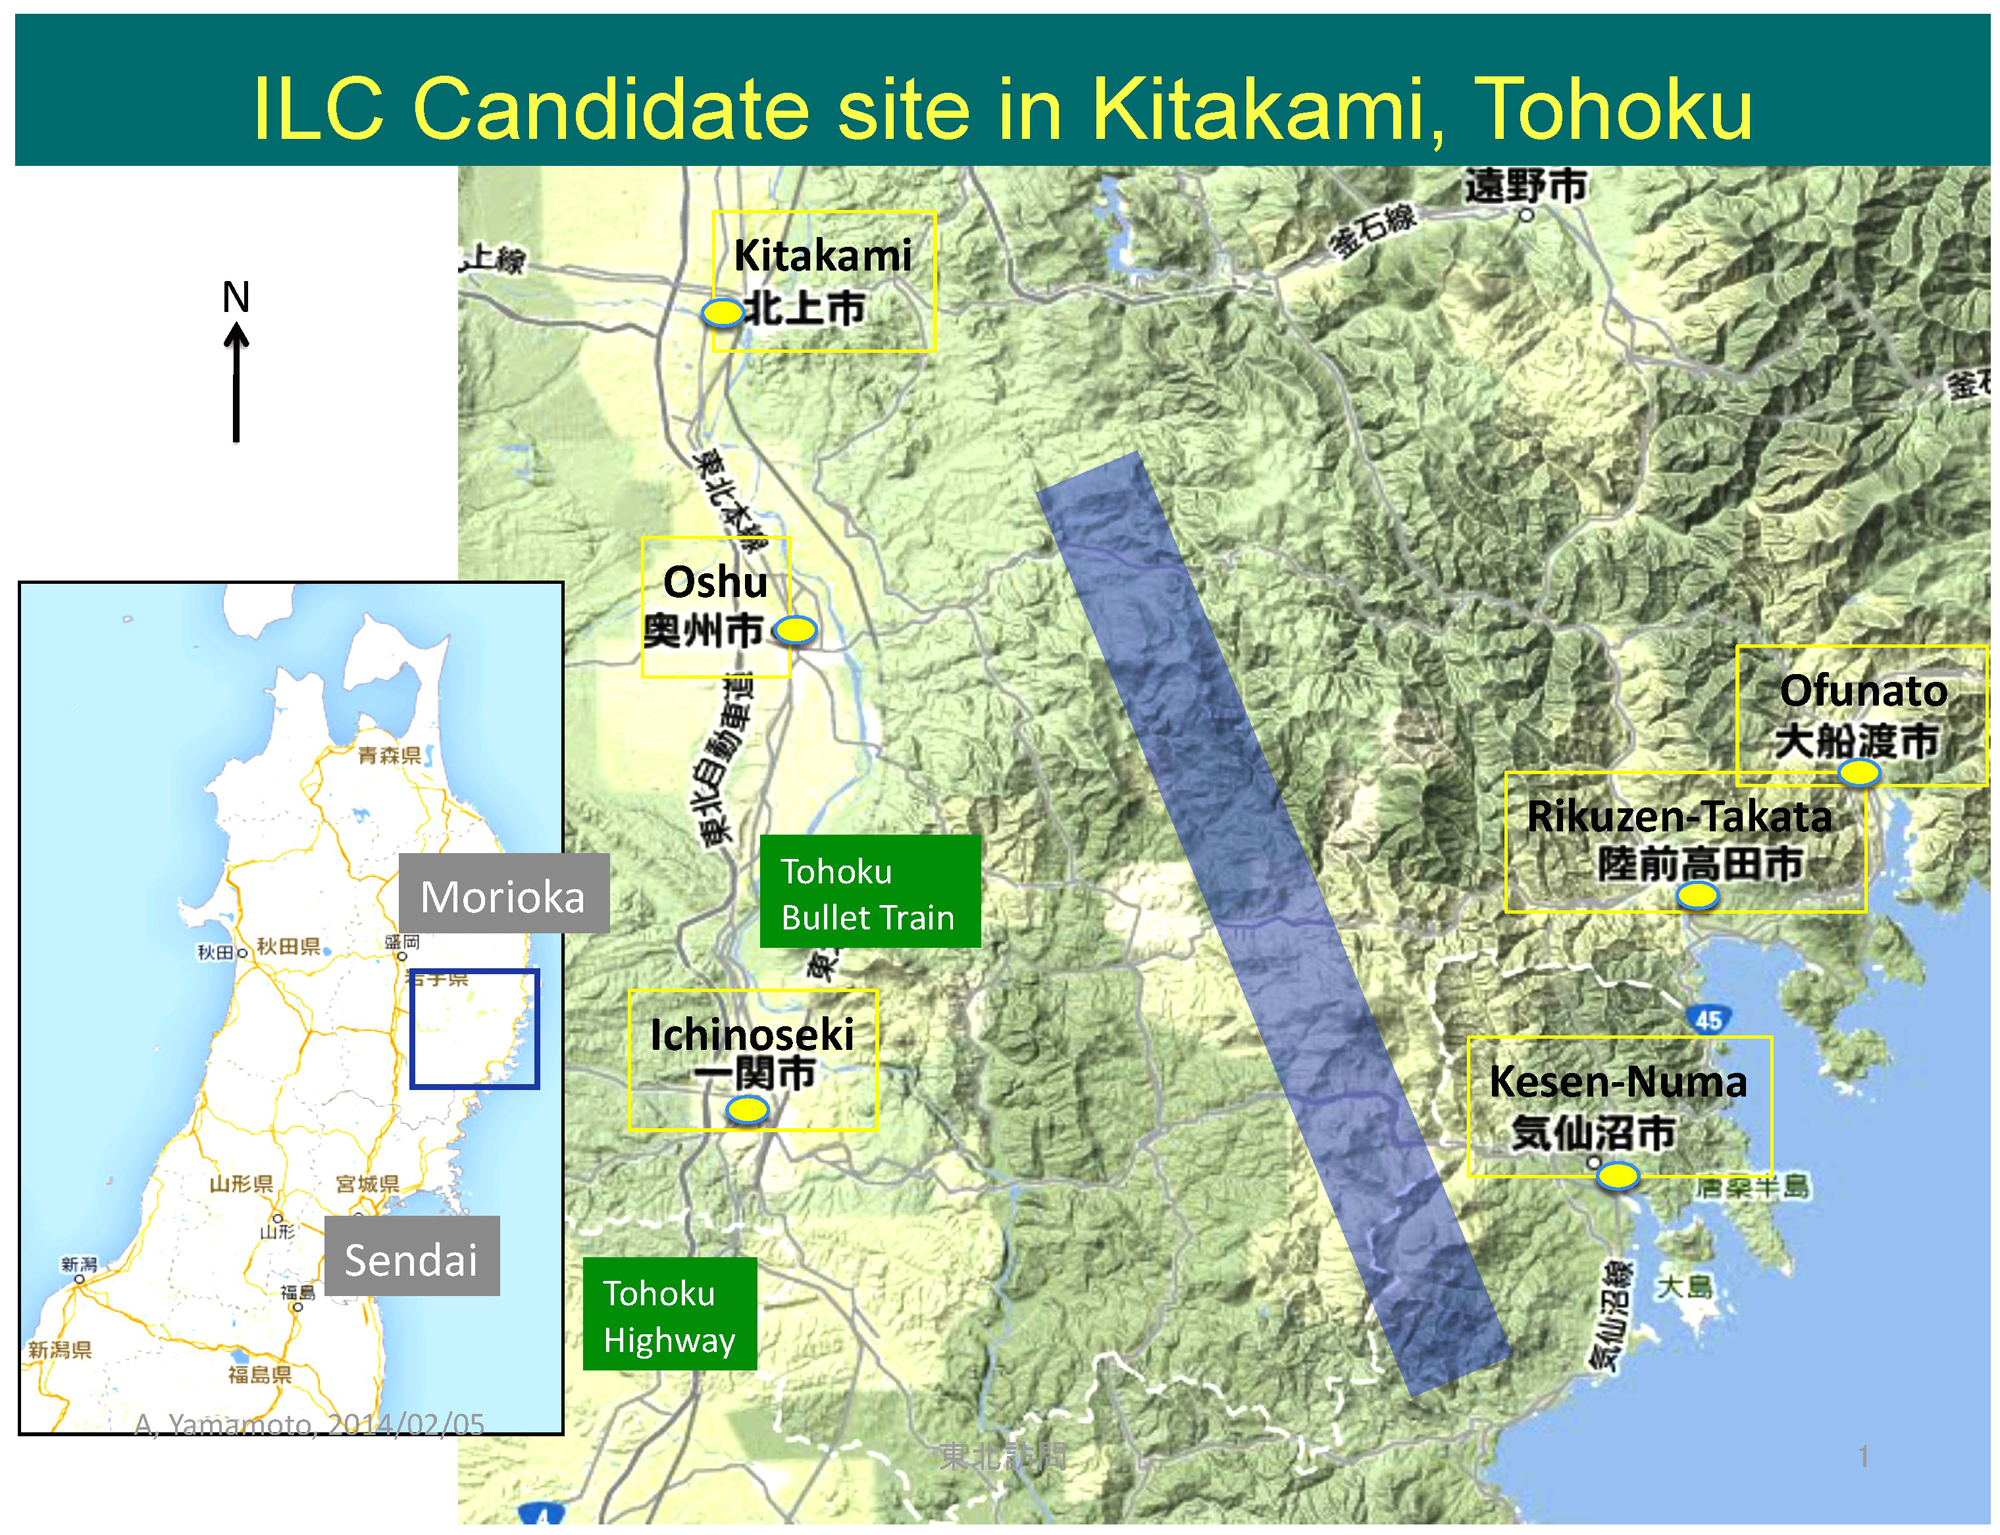
\includegraphics[width=\hsize]{chapters/figures/ILC-Candidate-Area2}
\caption{The Kitakami candidate site for the ILC~\cite{Warmbein:2014a}.}
\label{fig:kitakami-site}
\end{figure}

The site (Fig.~\ref{fig:kitakami-site}) is located in the Japan's northern Tohoku region, not far from Sendai with its international airport, in the prefectures of Iwate and Miyagi.
The closest cities are Ichinoseki, Oshu, and Kitakami, which all offer Shinkansen (bullet train) access to Sendai and Tokyo.
The closest harbour is in the city of Kesen-Numa.
The coastal region in this area was severely hit by the great Tohoku earthquake in 2011. 
Both prefectures are supportive of the ILC project and view it as an important part of their strategy to recover from the earthquake disaster.

The Kitakami site was largely selected because of its excellent geological condition. 
The proposed ILC trajectory lies in two large, homogeneous granite formations, the Hitokabe granite in the north and Senmaya granite to the south.
The site provides up to \siunit{50}{km} of space, enough for a possible \siunit{1}{TeV} upgrade or more, depending on the achievable accelerating gradient.  
Extensive geological surveys have been conducted in the area, including boring, seismic measurements, and electrical measurements~\cite{Sanuki:2015a}, as shown in Fig.~\ref{fig:kitakami-geology}.
The surveys show that the rock is of good quality, with no active seismic faults in the area.

Earthquakes are frequent throughout Japan, and the accelerator and detectors need  proper supports that isolate them from vibrations during earthquakes and micro tremors~\cite{Sanuki:2018b}. 
Proven technologies exist to cope with all seismic events, including magnitude 9 earthquakes such as the great Tohoku earthquake. 

% XXXXX MENTION TUNNELLING TECHNOLOGY (NAT), Cross section, Tomo's talk on earthquake vibes XXXXXXXX

Vibration measurements taken during the construction of a road tunnel show that accelerator operation would be possible during the excavation of a tunnel for an energy upgrade~\cite{Sanuki:2018a}.


% XXXXXXX CONTINUE HERE XXXXXXXXXX

\begin{figure}[htbp]
   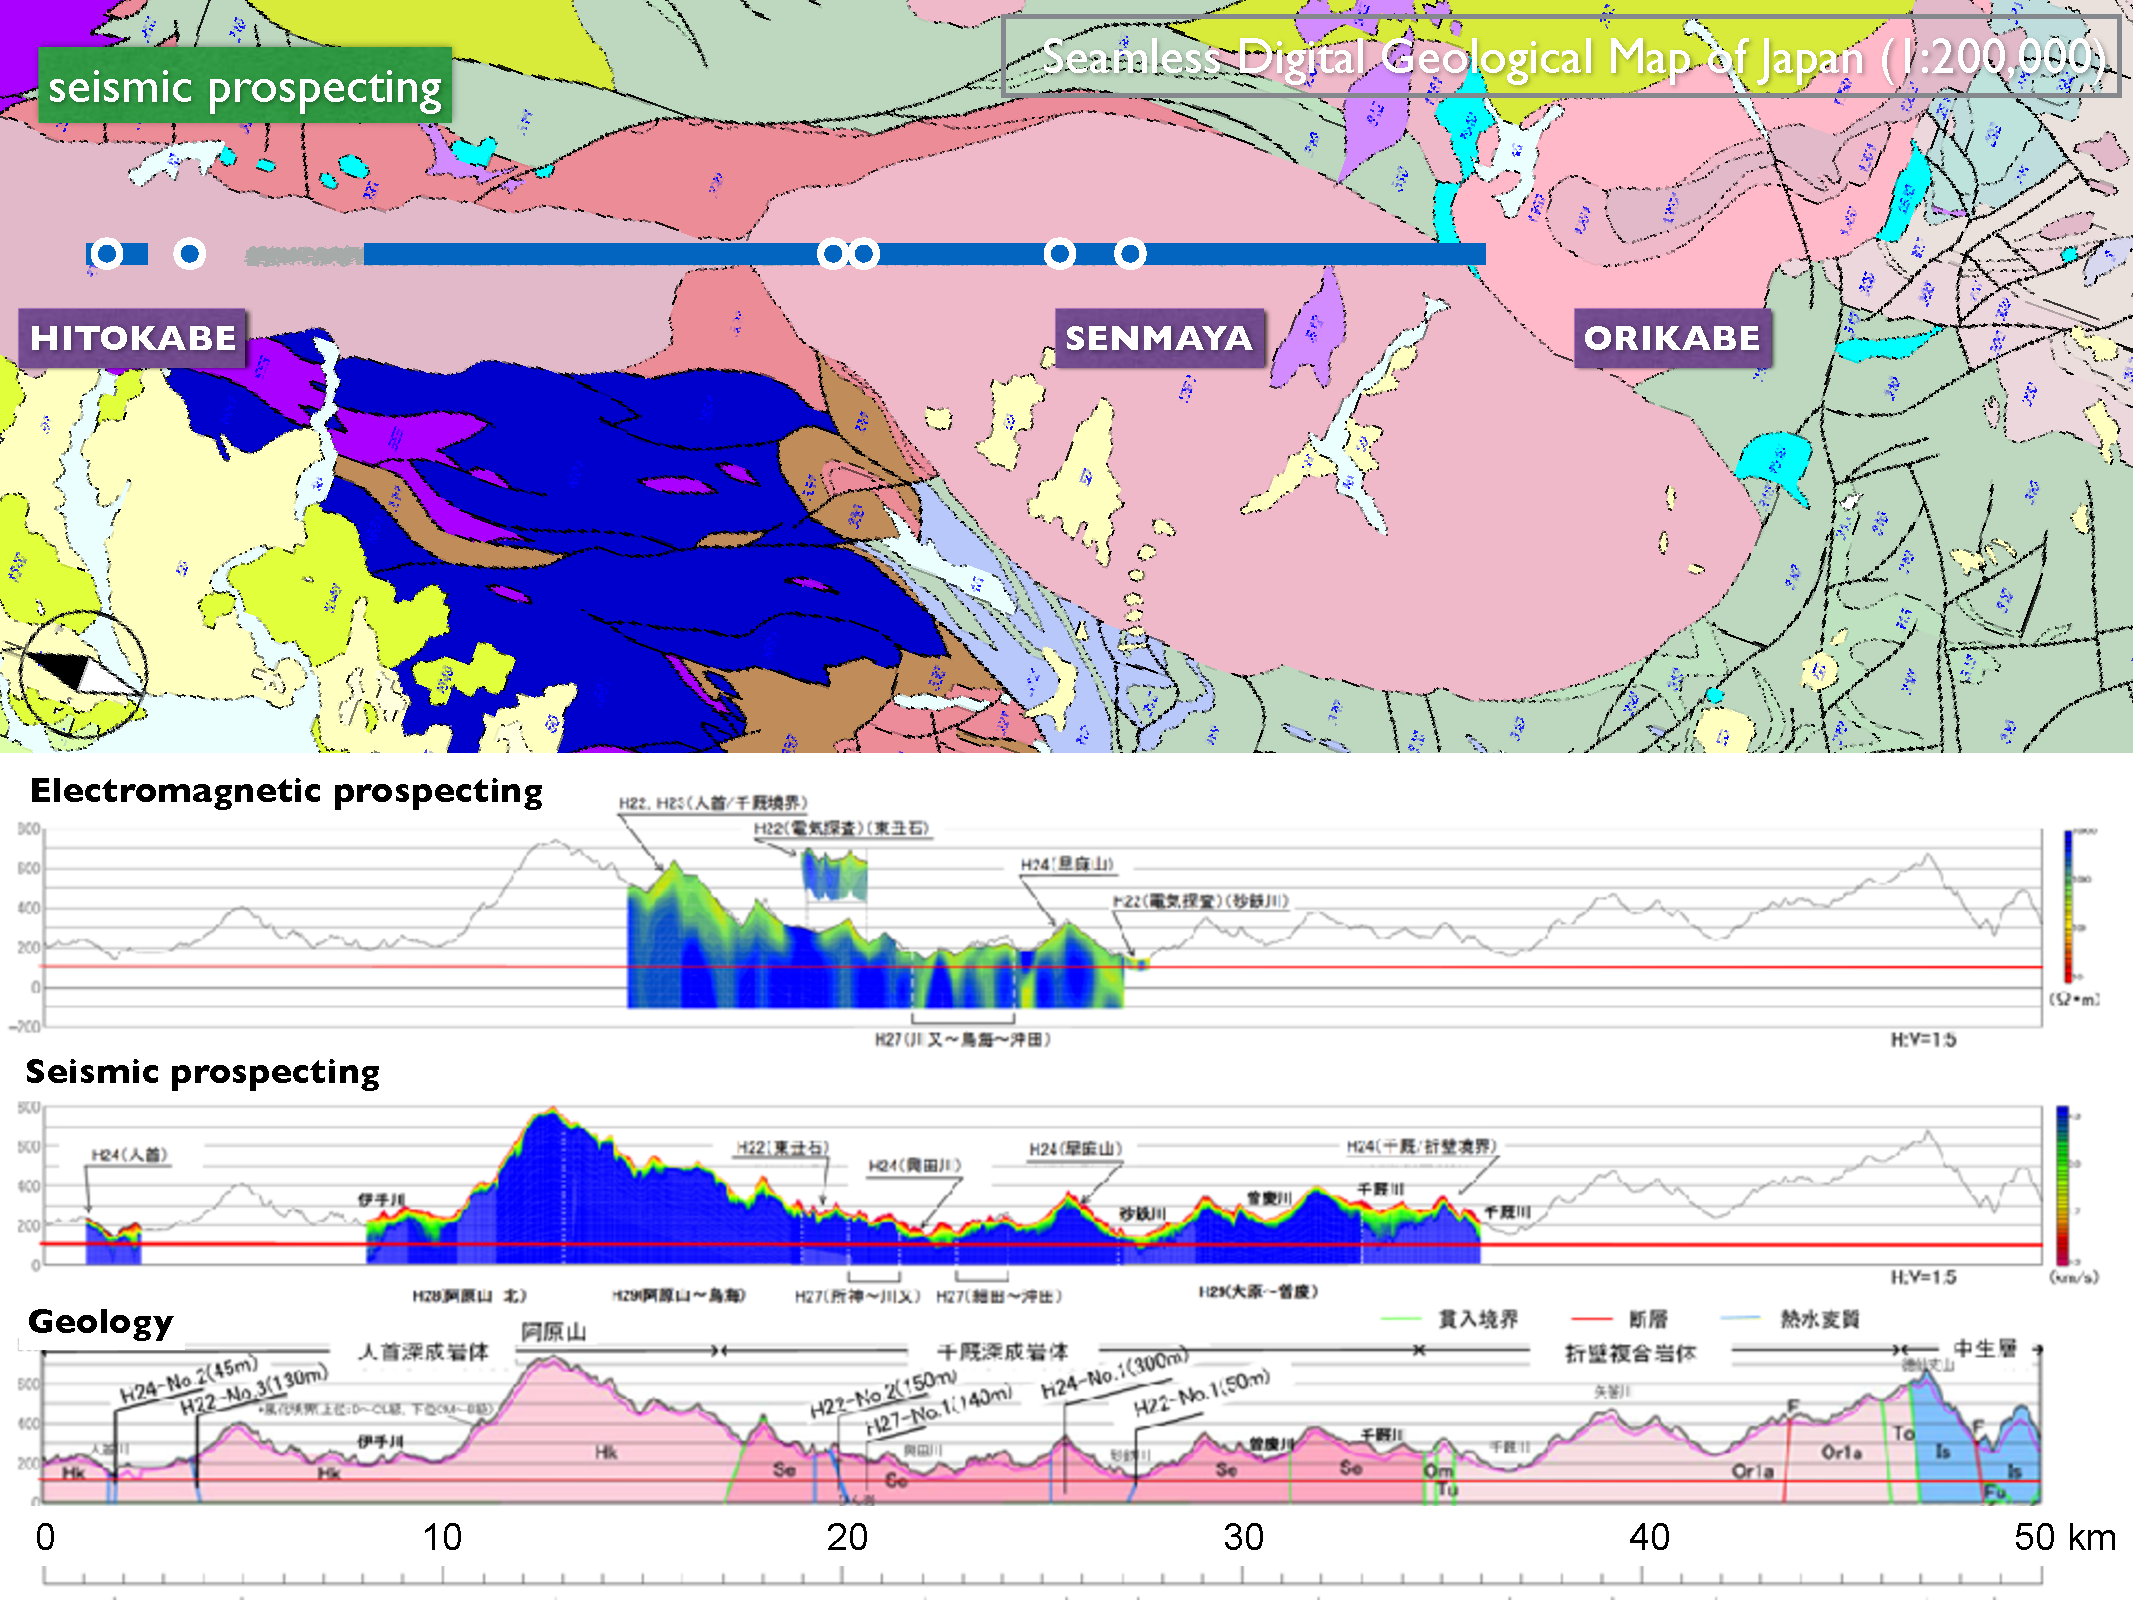
\includegraphics[width=\hsize]{chapters/figures/Kitakami_Geology}
\caption{Geological situation at the Kitakami site.}
\label{fig:kitakami-geology}
\end{figure}


%===============================================================================

\begin{figure*}[htbp]
 %\epsfysize=9.0cm
 \begin{center}
 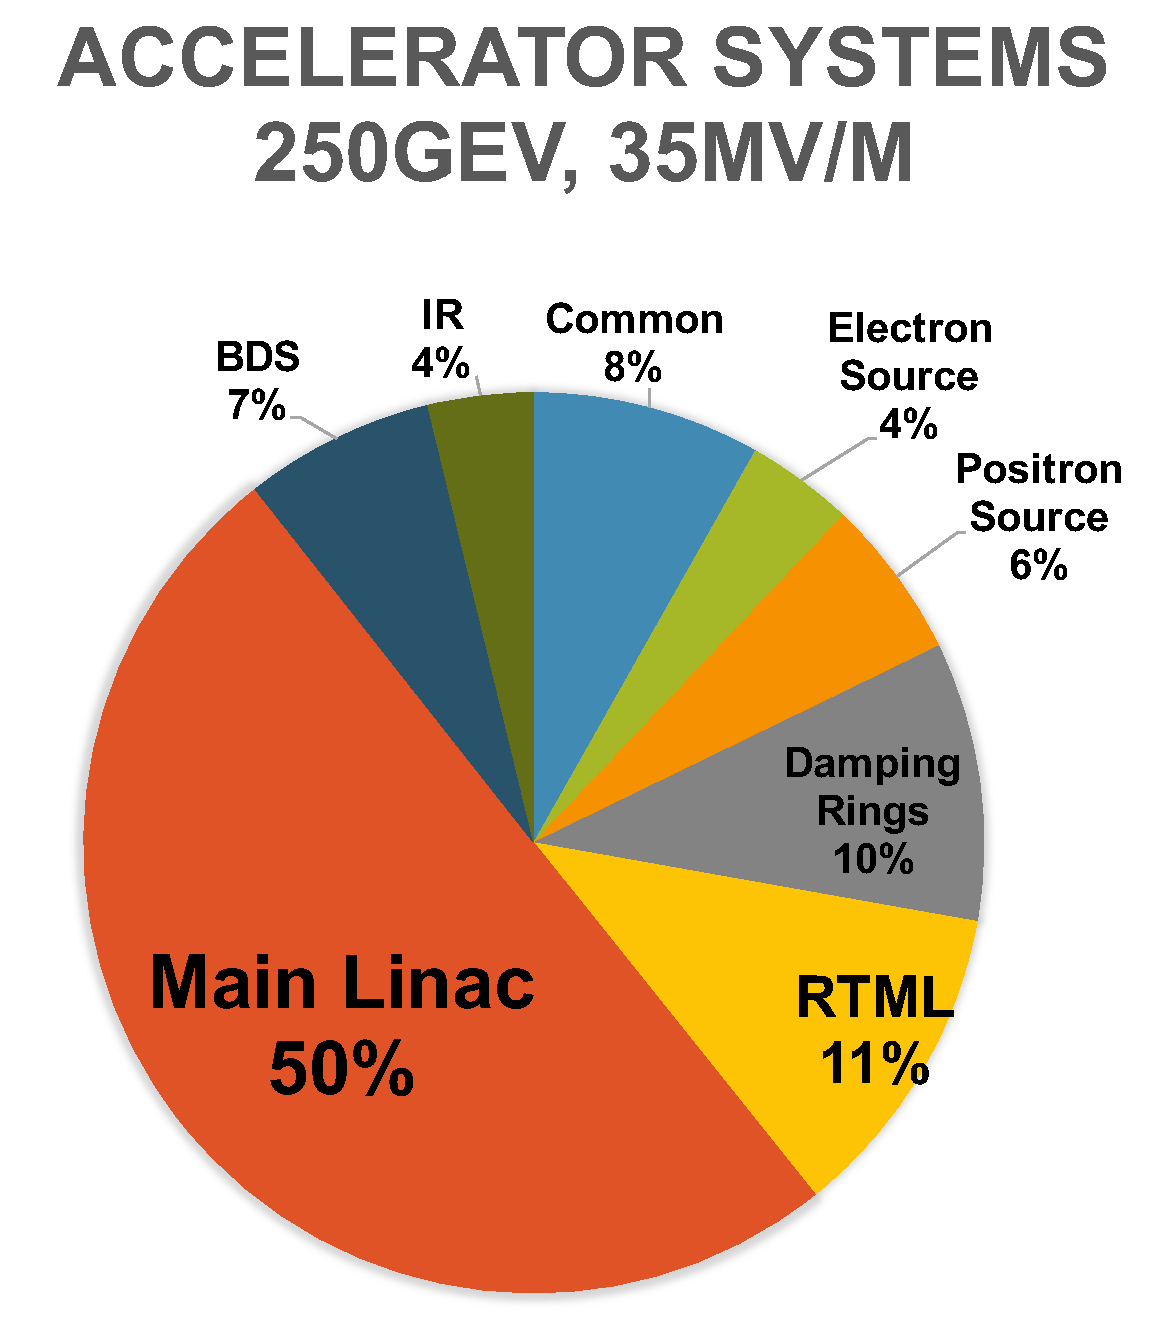
\includegraphics[width=0.36\hsize]{chapters/figures/costs-as.pdf}
 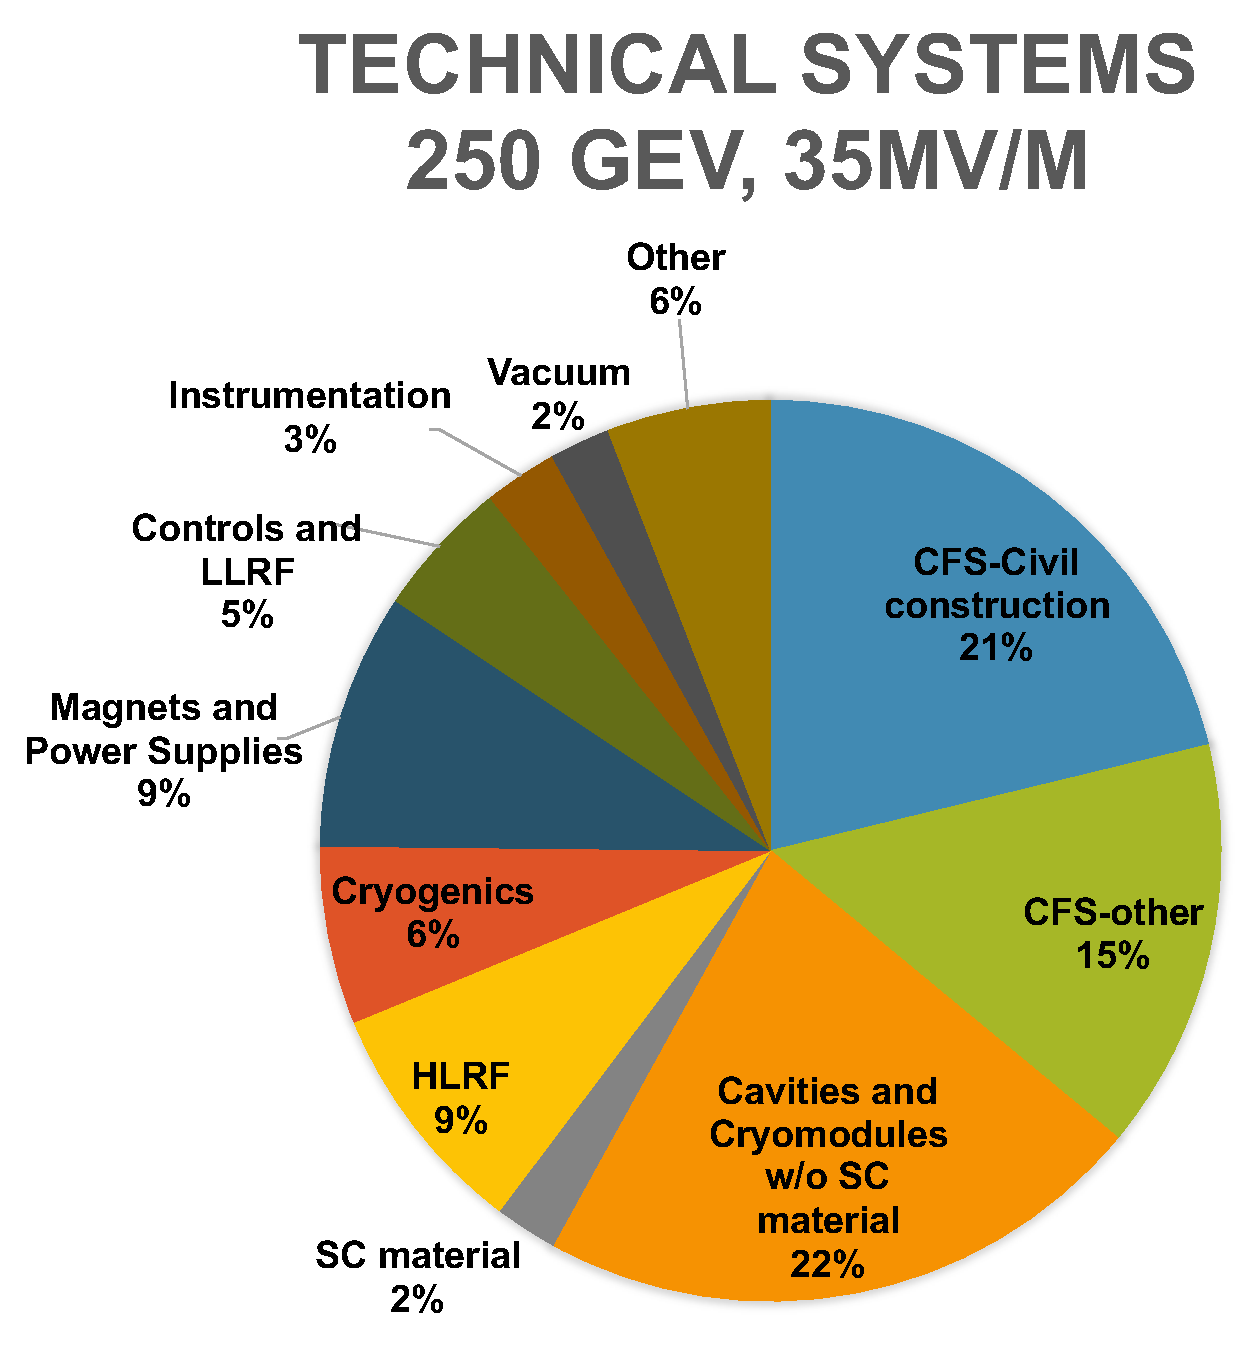
\includegraphics[width=0.4\hsize]{chapters/figures/costs-ts.pdf}
\caption{Breakdown of Value costs into accelerator systems (left) and technical systems (right) for the \siunit{250}{GeV} ILC accelerator, assuming that cost reduction measures are successful and a gradient of \siunit{35}{MV/m} can be reached.
\label{fig:costs}}
 \end{center}
 \end{figure*}


\subsection{Cost and Schedule}


%{\it 
%Description of Cost estimate and schedule - 1 page 
%
%include human resources, cost reduction effect by R\&D, operating costs
%}

For the Technical Design Report, the construction cost of the ILC accelerator was carefully evaluated from a detailed, bottom--up, WBS (Work Breakdown Structure)-based cost estimation~\cite[Sect. 15]{Adolphsen:2013kya}.
The TDR estimate distinguishes two cost categories: Value accounts for materials and supplies procured from industry and is given in ILCU (ILC Currency Unit, where $\siunit{1}{ILCU} = \siunit{1}{US\$}$ in 2012 prices), and Labour accounts for work performed in the participating institutions and is given in person--hours or person--years\footnote{One person--year corresponds to $1700$ working hours.}.

The Value of acquired goods reflects its worth in the local currency of the purchasing institution. 
Therefore, conversion of Value between currencies is performed based on Purchasing Power Parities (PPP), which are regularly evaluated and published by the OECD~\cite{OECD:2018,Eurostat:2012}, rather than currency exchange rates. 
The PPP values reflect local price levels and thus depend on the type of goods and the country, but fluctuate significantly less than currency exchange rates.
Therefore, conversions from ILCU to other currencies cannot not be made on the basis of exchange rates to the U.S. dollar, but on PPP values.

The TDR cost estimate covers the cost of the accelerator construction, assumed to last 9 years plus one year of commissioning. 
It includes the cost for the fabrication, procurement, testing, installation, and commissioning of the whole accelerator, its components, and the tunnels, buildings \etc, and the operation of a central laboratory at the site over the construction period. 
It does not, however, not cover costs during the preparation phase preceding the start of construction work (``ground breaking''), such as design work, land acquisition, infrastructure (roads, electricity, water) for the site.

Based on the TDR cost estimate, an updated cost estimate was produced for the \siunit{250}{GeV} accelerator. 
This updated cost estimate includes the cumulative effect of the changes to the design since the TDR (see Sect.~\ref{sec:design_evo}), and evaluates the cost for the reduced machine by applying appropriate scaling factors to the individual cost contributions of the TDR cost estimate.

The resulting Value estimate for the ILC accelerator at \siunit{250}{GeV} is 
\siunit{4,780-5,260}{MILCU}~\cite{Evans:2017rvt} in 2012 prices, where the lower number assumes a cavity gradient of \siunit{35}{MV/m}, while the higher number is based on the TDR number of \siunit{31.5}{MV/m}. 
In addition, \siunit{17,165}{kh} (thousand person-hours) are required of institutional Labour.

In 2018, the ILC Advisory Panel of the Japanese Ministry of Education, Culture, Sports, Science and Technoloy (MEXT) concluded its review of the ILC~\cite{ILCAP:2018}. 
For this review, costs were evaluated in Japanese Yen in 2017 prices, taking into account the local inflation for goods and construction costs.
For the purpose of this estimate, also the Labour costs were converted to Yen to yield \siunit{119.8}{G\yen}, resulting in a total range of the accelerator construction cost of \siunit{635.0 - 702.8}{G\yen}, where the range covers uncertainties in the civil construction costs (\siunit{18}{G\yen}) and of the gradient (\siunit{49.8}{G\yen}).
For the this estimate, conversion rates of $\siunit{1}{US\$} = \siunit{100}{JP\yen}$ and $\siunit{1}{\matheuro} = \siunit{1.15}{US\$}$ were assumed.

Operation costs of the accelerator and the central laboratory are estimated to be \siunit{36.6-39.2}{G\yen} (about \siunit{318-341}{M\matheuro}) per year.

% XXXXXX DISCUSS EFFECT OF COST REDUCTION R&D XXXXXX

% XXXXXX uncertainty, contingency, risk, running costs

% XXXXXX CONTINUE HERE WITH SCHEDULE   XXXXXXX













  
\section{\label{sec:runscenarios}ILC Running Scenarios  }
   5 pages J. List
   
%  section on run scenarios

% CHAPTER ON ILC RUNNING SCENARIOS

One of the key advantages of $e^+e^-$ colliders is the ability to collect individual datasets at at a series of different center-of-mass energies and beam polarisation settings.   While each measurement one might wish to make has its own prefered data-taking mode, the combination with datasets collected at other beam energies and/or beam polarisations provides a unique robustness against systematic uncertainties.  This is obvious for data-taking at different energies, but it is also
true for data-taking at different polarizations. For example, a recent PhD thesis~\cite{Habermehl:417605} studied Dark Matter searches with consideration of  non-neglibigle systematic uncertainties and showed that one obtains better results by  sharing a given amount of total integrated luminosity between datasets with different beam polarisations rather than by investing the same total amount of luminosity into the (statistically) most favourable polarisation configuration.

Any physics projection will therefore depend on the exact running scenario, i.e.\ the ensemble of the integrated luminosities collected at the individual center-of-mass energies with the various polarisation settings. For the physics conclusions given in this paper, we have assumed the energy and luminosity evolution of the ILC shown 
in Fig.~\ref{fig:H20staged}.  At each energy, the time is shared among the various choices for beam polarization in the manner explained in Sec.~\ref{subsec:runscen_pol}.
The full physics program is projected to take 22 years, including a realistic learning 
curve for the establishment of luminosity and scheduled downtimes for luminosity and energy upgrades.   In this schedule, the ILC would accumulate 2\,ab$^{-1}$ at 250\,GeV by year 11.  It woud then add datasets of 0.2\,ab$^{-1}$ at 350\,GeV and  4\,ab$^{-1}$ at 500\,GeV by year 22. 

%%%%%%%%%%%%%%%%%%%%%%%%%%%%%%%%%%%%%%%%%%%%%%%%%%%%%%%%%%%%%%%%%%%%%%%%%
\begin{figure}
\begin{center}
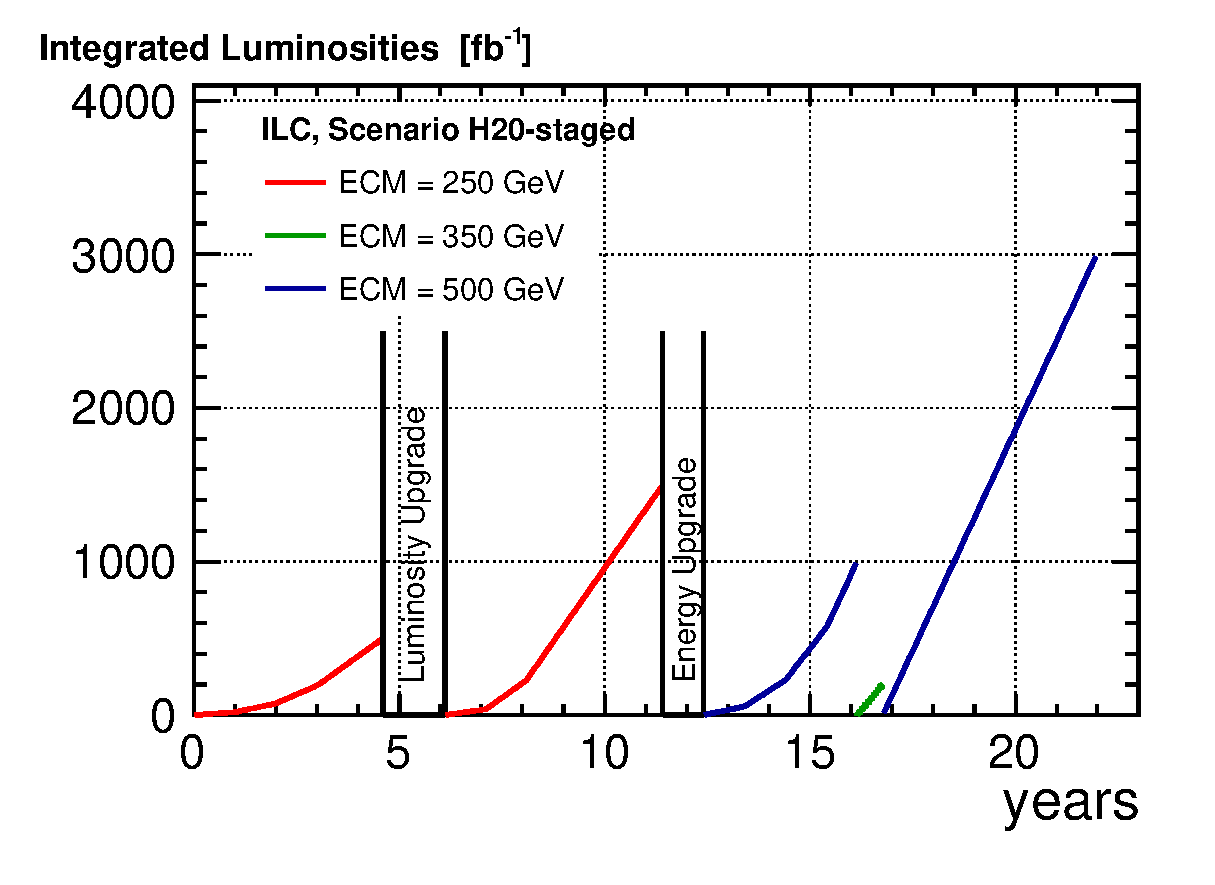
\includegraphics[width=0.90\hsize]{chapters/figures/lumi_H20-staged}
\end{center}
\caption{The nominal 22-year running program for the staged ILC, starting operation at 250\,\GeV with the current baseline beam parameters for the 250\,GeV runs~\cite{Fujii:2017vwa}. }
\label{fig:H20staged}
\end{figure}
%%%%%%%%%%%%%%%%%%%%%%%%%%%%%%%%%%%%%%%%%%%%%%%%%%%%%%%%%%%%%%%%%%%%%%%%%%%


The interplay between different datasets has been studied in detail in~\cite{Barklow:2015tja}, with a special focus on the optimisation of the Higgs precision measurements, resulting in a standard running scenario for ILC physics projections. The time evolution of this running scenario has been adapted to the staged construction of the ILC as first presented in~\cite{Fujii:2017vwa}. 

In this section, we will discuss the considerations that have entered the choice of this running scenario, the evolution of this scenario in accord with the design of the 
ILC accelerator, and the flexibility of the plan to respond to changes in machine
specifications or physics discoveries.

\subsection{Center-of-mass energies and integrated luminosities}
The three center-of-mass energies for ILC best motivated by our current knowledge are:
\begin{itemize}
\item $\sqrt{s}=250$\,GeV for collecting data near the threshold of the Higgsstrahlungs process, 
\item $\sqrt{s}=350$\,GeV for scanning the threshold for top quark pair production, and 
\item $\sqrt{s}=500$\,GeV or somewhat above for studying $t\bar{t}$ production in the continuum and enabling $t\bar{t}H$ and $ZHH$ production. 
\end{itemize}
Table~\ref{tab:lumiabstot} gives the total integrated luminosities foreseen at these energies for three alternative running scenarios.  These scenarios are described in~\cite{Barklow:2015tja},  which presented a detailed evaluation of these and other possibilities.  For comparison,  the integrated luminosities assumed in the Snowmass community study~\cite{Asner:2013psa}  is given in the last column. Since 2015, the scenario H20 has been  the reference scenario for ILC physics projections.

\begin{table}[h]
\centering
  \renewcommand{\arraystretch}{1.10}
\begin{tabularx}{\columnwidth}{*{4}{>{\centering\arraybackslash}X} || *{1}{>{\centering\arraybackslash}X}} 
%\begin{tabular*}{\textwidth}{@{\extracolsep{\fill}}c|c c c c c}
%\begin{tabular}{|l||c|c|c|c|c|}
\hline
            &  \multicolumn{4}{c}{$\int{\mathcal{L} dt}$ [fb$^{-1}$]} \\
\hline
$\sqrt{s}$  & G20      &   H20   &  I20   & Snow   \\
\hline
250\,GeV    &  500      &  2000    &   500   & 1150   \\
350\,GeV    &  200      &   200    &  1700   &  200  \\
500\,GeV    & 5000      &  4000    &  4000   & 1600  \\
\hline
%\end{tabular*}
\end{tabularx}
\caption{Proposed total target integrated luminosities for $\sqrt{s}=250$,  $350$, $500$\,GeV based on $20$ ``real-time'' years of ILC operation under scenarios G20, H20 and I20. The total integrated luminosities assumed for Snowmass
are listed for comparison based on 13.7 ``real-time'' years. From~\cite{Barklow:2015tja}.}
\label{tab:lumiabstot} 
\end{table}


It must be stressed, however, that flexibility in the run plan remains one of the key assets of the ILC.  This plan can be adjusted whenever new insights,  discoveries either from the (HL-)LHC or from the ILC itself, require us to do so. In particular, the center-of-mass energy of the ILC can always be lowered from the nominal maximum energy without loss of efficiency and/or luminosity, as long as the electron beam energy remains sufficiently high for positron production. In fact, the operation of the SCRF cavities below the maximum gradient
saves significant cryogenic and RF power, which in turn can be invested into higher instantaneous luminosity.

Future $e^+e^-$ colliders could also provide important physics measurements at other center-of-mass energies. Physics goals that motivate other choices are the high-statistics study of $Z$ and $W$, the exploration of the thresholds for any new color-singlet particles that might appear in the ILC energy region, and data-taking at additional center of mass energies to optimize the determination of Effective Field Theory parameters. The lower center-of-mass energies could be realized by doubling the repetition rate of the electron linac to 10\,Hz and adding a by-pass around the positron source for every second bunch train. Today, however, the priority of these issues seems lower than that  for the abovementioned three energies. Therefore they are not explicitly included in the current run plan of the ILC or in the current set of machine parameters.  Over a longer term, we plan to extend the linac to reach 
energies of 1\,TeV or higher.   Table~\ref{tab:lumiabstot1TeV} lists target integrated luminosities approriate to physics studies at these additional energies.

\begin{table}[h]
\centering
  \renewcommand{\arraystretch}{1.10}
\begin{tabularx}{\columnwidth}{l *{4}{>{\centering\arraybackslash}X}} 
%\begin{tabular*}{\textwidth}{@{\extracolsep{\fill}}c|c c c c c}
%\begin{tabular}{|l||c|c|c|c|c|}
\hline
$\sqrt{s}$     &  90\,GeV & 160\,GeV  &    1\,TeV \\
\hline
 $\int{\mathcal{L} dt}$ [fb$^{-1}$]         	   &  100       &  500    & 8000 \\
\hline
%\end{tabular*}
\end{tabularx}
\caption{Proposed total target integrated luminosities for other $\sqrt{s}$.  From~\cite{Barklow:2015tja}.}
\label{tab:lumiabstot1TeV} 
\end{table}


\subsection{Beam polarisation}
\label{subsec:runscen_pol}
At center-of-mass energies of up to 500\,GeV, the ILC beams are foreseen to be polarised  with absolute values of at least 80\% for the electrons and at least 30\% for the positrons. At 1\,TeV, the positron polarisation will reach at least 20\%. As an upgrade option, the positron polarisation can be increased to 60\% for center-of-mass energies around 500\,GeV; this is discussed in Sec.~\ref{subsubsec:upg-optP}. The accelerator design comprises sets of spin rotators which in principle allow one to prepare any desired direction of the polarisation vectors at the IP. However in the detailed running scenarios, we consider only longitudinal polarisation. The sign of the beam polarisations can be flipped 
on a train-by-train basis. This allows us to collect datasets with different helicity configurations quasi-concurrently compared to the typical time scales of changes in the accelerator or detector configuration, calibration and alignment. In a joint analysis of these datasets, large parts of the experimental systematic uncertainties cancel.  This is particularly important to minimize the 
systematic errors in the measurement of the left-right polarization asymmetry, a quantity that carries a great deal of information for every process that will be studied at the ILC.  But this idea has many other applications. The joint interpretation of the different datasets allows us to treat many systematic effects as nuisance parameters in global fits, and thereby to measure and subtract these effects~\cite{bib:PhDRobert}. 

The role of positron polarisation specifically at an initial 250-GeV stage of the ILC has been discussed in detail in a recent document~\cite{Fujii:2018mli}. In the case of a global fit to polarised total and differential cross-sections of various electroweak processes, it is shown there  that the uncertainties on some observables increase by up to a factor of 10 in the absence of positron polarisation due to the lack of redundancies required for ultimate control of systematic uncertainties. As we will see in Sec.~\ref{subsec:phys_eft}, the left-right asymmetry $A_{LR}(HZ)$ of the Higgsstrahlungs cross section plays an important role in our technique for obtaining a  model-independent fit to Higgs couplings.  Although the measurement of the absolute normalization of the Higgsstrahlungs cross section was not explicitly included in the study summarized in~\cite{Fujii:2018mli}, analogous deteriorations would also be expected for this quantity.

A part of the power of positron polarisation is that it allows one to collect four independent data sets with different mixtures of the physics reactions under study.   Tables~\ref{tab:pollumirel} through~\ref{tab:pollumiabs1TeV} give our
standard assumptions for the sharing of the total integrated luminosity (c.f.\ Tab.~\ref{tab:lumiabstot} and~\ref{tab:lumiabstot1TeV}) between the four possible beam helicity combinations. Due to the importance of  $A_{LR}(HZ)$~\cite{Durieux:2017rsg, Barklow:2017suo} noted above, the sharing for 250\,GeV, which was originally foreseen~\cite{Barklow:2015tja} to emphasize the $\operatorname{sgn}(P(e^-),P(e^+))=(-,+)$ configuration, is now  adjusted to provide equal amounts of luminosity for $(-,+)$ and $(+,-)$~\cite{Barklow:2017suo, Fujii:2017vwa}.

These integrated luminosities and polarisation configurations, especially as specified in Tab.~\ref{tab:pollumiabs} for the H20 running scenario, define the reference scenario for all ILC physics projections.  The order in which the various energies are surveyed will of course depend on the machine evolution and staging plan.

\begin{table}[h]
\centering
  \renewcommand{\arraystretch}{1.10}
\begin{tabularx}{\columnwidth}{l *{4}{>{\centering\arraybackslash}X}} 
%\begin{tabular*}{\textwidth}{@{\extracolsep{\fill}}|c|c|c|c|c|c|}
%\begin{tabular}{|l||c|c|c|c|c|}
\hline
        & \multicolumn{4}{c}{fraction with $\operatorname{sgn}(P(e^-),P(e^+))= $ } \\
           & (-,+) & (+,-) & (-,-) & (+,+) \\
\hline
$\sqrt{s}$ & [\%]  &  [\%] & [\%]  & [\%]  \\ 
\hline
250\,GeV (2015)   & 67.5 &  22.5 &  5    &   5   \\
250\,GeV (update) & \bf{45} &  \bf{45} &  5    &   5   \\
350\,GeV   & 67.5 &  22.5 &  5    &   5   \\
500\,GeV   &  40  &  40   &  10   &  10   \\
\hline
%\end{tabular*}
\end{tabularx}
\caption{Relative sharing between beam helicity configurations proposed for the various center-of-mass energies. The update of the luminosity
sharing for 250\,GeV originates from the importance of the left-right asymmetry of the Higgsstrahlung cross section in the EFT-based Higgs coupling fit.}
\label{tab:pollumirel} 
\end{table}

\begin{table}[h]
\centering
  \renewcommand{\arraystretch}{1.10}
\begin{tabularx}{\columnwidth}{l *{4}{>{\centering\arraybackslash}X}}    %\begin{tabular*}{\textwidth}{@{\extracolsep{\fill}}|c|c|c|c|c|}
%\begin{tabular}{|l|c|c|c|c|}
\hline
        &  \multicolumn{4}{c}{int. luminosity with $\operatorname{sgn}(P(e^-),P(e^+))= $ } \\
           & (-,+)       & (+,-)       & (-,-)       &  (+,+)     \\
\hline
$\sqrt{s}$ & [fb$^{-1}$] & [fb$^{-1}$] &  [fb$^{-1}$] & [fb$^{-1}$] \\ 
\hline
250\,GeV (2015)   &  1350      &  450        &  100	      &   100  \\
250\,GeV (update) &  \bf{900}  &  \bf{900}   &  100	      &   100  \\
350\,GeV          &   135      &   45	     &   10	      &    10  \\
500\,GeV          &  1600      & 1600        &  400	      &   400  \\
\hline
\end{tabularx}
\caption{Integrated luminosities per beam helicity configuration resulting from the fractions in table~\ref{tab:pollumirel} in scenario H20. The update of the luminosity
sharing for 250\,GeV originates from the importance of the left-right asymmetry of the Higgsstrahlung cross section in the EFT-based Higgs coupling fit. 
}
\label{tab:pollumiabs} 
\end{table}

\begin{table}[h]
\centering
  \renewcommand{\arraystretch}{1.10}
\begin{tabularx}{\columnwidth}{l *{4}{>{\centering\arraybackslash}X}} 
%\begin{tabular*}{\textwidth}{@{\extracolsep{\fill}}|c|c|c|c|c|c|}
%\begin{tabular}{|l||c|c|c|c|c|}
\hline
        & \multicolumn{4}{c}{fraction with $\operatorname{sgn}(P(e^-),P(e^+))= $ } \\
           & (-,+) & (+,-) & (-,-) & (+,+) \\
\hline
$\sqrt{s}$ & [\%]  &  [\%] & [\%]  & [\%]  \\ 
\hline
90\,GeV    &  40  &  40   &  10   &  10   \\
160\,GeV   & 67.5 &  22.5 &  5    &   5   \\
1\,TeV     &  40  &  40   &  10   &  10   \\
\hline
%\end{tabular*}
\end{tabularx}
\caption{Relative sharing between beam helicity configurations proposed for low energy and $1$\,TeV running. From~\cite{Barklow:2015tja}.}
\label{tab:pollumirel1TeV} 
\end{table}

\begin{table}[h]
\centering
  \renewcommand{\arraystretch}{1.10}
\begin{tabularx}{\columnwidth}{l *{4}{>{\centering\arraybackslash}X}}    %\begin{tabular*}{\textwidth}{@{\extracolsep{\fill}}|c|c|c|c|c|}
%\begin{tabular}{|l|c|c|c|c|}
\hline
        &  \multicolumn{4}{c}{integrated luminosity with $\operatorname{sgn}(P(e^-),P(e^+))= $ } \\
           & (-,+)       & (+,-)       & (-,-)       &  (+,+)     \\
\hline
$\sqrt{s}$ & [fb$^{-1}$] & [fb$^{-1}$] &  [fb$^{-1}$] & [fb$^{-1}$] \\ 
\hline
90\,GeV     &    40   	 &   40        &   10	      &    10  \\
160\,GeV    &   340   	 &  110        &   25	      &    25  \\
1\,TeV      &  3200   	 & 3200        &  800	      &   800  \\
\hline
\end{tabularx}
\caption{Integrated luminosities per beam helicity configuration resulting from the fractions in table~\ref{tab:pollumirel1TeV}. From~\cite{Barklow:2015tja}.}
\label{tab:pollumiabs1TeV} 
\end{table}


\subsection{Time Evolution and Upgrade Options}

The possible real-time evolution of the integrated luminosity was studied in detail in~\cite{Barklow:2015tja}.  It is important to note that the plans given in that study assumed that the full 500\,GeV machine would be available from the beginning. With the introduction of a staged construction plan for the ILC, the time ordering of 
different runs needed to be adjusted. However, the details of trade-offs between scenarios is most fully documented in 
\cite{Barklow:2015tja}, so we will first review that study and the logic of its conclusions.   After this, we will describe our
current plan for the run scenario including the constraints from staging. 

\subsubsection{Running Scenarios for the 500-GeV Machine}
\label{subsubsec:runscen_ilc500}

In the study \cite{Barklow:2015tja}, the peak luminosities used for each centre-of-mass energy are based on the numbers published in the ILC TDR~\cite{Adolphsen:2013jya}. But then, the plans took advantage of the reduced linac  electrical power and cryogenic loads when operating the full 500\,GeV machine at lower gradients.  This in particular allows 10-Hz and 7-Hz running, respectively, at the 250\,GeV  and 350\,GeV centre-of-mass energies. In addition, a luminosity upgrade (from 1312 to 2625 bunches per pulse) was been considered; this could require the installation of an additional positron damping ring, as described in  Sec.~\ref{subsubsec:upg-optL}.

More specifically, the study \cite{Barklow:2015tja} made the following assumptions:

\begin{itemize} 
\item A full calendar year is assumed to represent eight months running at an efficiency of 75\% as assumed in the ILC RDR~\cite{Phinney:2007gp}. This corresponds approximately to $Y= 1.6 \times 10^7$ seconds of integrated
running, thus 60\% more than a ``Snowmass year'' of $10^7$ seconds.
\item The start of ``Year 1'' is the start of running for physics. After the end of construction, there is one year foreseen for machine commissioning only, which is not shown on the plots.
\item A ramp-up of luminosity performance, defined as a set of yearly ramp factors $f \le 1$, is in general assumed after: (a) initial construction and `year 0' commissioning; (b) a downtime for a luminosity upgrade; (c) a change in operational mode which may require some learning curve (\eg,  going to 10-Hz collisions).
\item If the peak instantaneous luminosity is $L$, then the nominal integrated luminosity for any given
calendar year is $\int \mathcal{L} dt = f \times L \times Y$, where $f$ is the ramp factor associated with that year.
\item The peak instantaneous luminosities are those corresponding to the TDR beam parameters at 250, 350 and 500\,GeV, as shown in Tab.~\ref{tab:ilc-params}.
\item For the initial physics run after construction and year 0 commissioning, the RDR ramp of 10\%,
30\%, 60\% and 100\% over the first four calendar years is always assumed.
\item  The ramp after the shutdown for installation of the luminosity upgrade is assumed to be slightly shorter (10\%, 50\%, 100\%) with no year 0.
\item Going down in centre of mass energy from $500$\,GeV to $350$\,GeV or $250$\,GeV is assumed to have no ramp
associated with it, since there is no modification (shutdown) of  the machine. 
\item Going to 10-Hz operation at 50\% gradient does assume a ramp however (25\%, 75\%, 100\%),
since 10-Hz affects the entire machine including the damping rings and sources.

\end{itemize}


Under these assumption, a possible real-time scenario for collecting
the integrated luminosities of the H20 scenario (c.f. Tab~\ref{tab:lumiabstot}) is shown in Fig.~\ref{fig:H20}. Since 
it was assumed that the full 500-GeV machine would be available from the start, the first foreseen run was intended to collect a dataset of 500\,fb$^{-1}$ at $\sqrt{s}=$500\,GeV in order to observe for the first time ever $t\bar{t}$ production via the electroweak force,
to survey the full kinematic reach for possible new particles and, last but not least, to collect a comprehensive set of Higgs precision data, with similar contributions from the Higgsstrahlung and $WW$ fusion processes (see \ Fig.~\ref{fig:HiggsProdILC}). 

%%%%%%%%%%%%%%%%%%%%%%%%%%%%%%%%%%%%%%%%%%%%%%%%%%%%%%%%%%%%%%%%%%%%%%%%%
\begin{figure}
\begin{center}
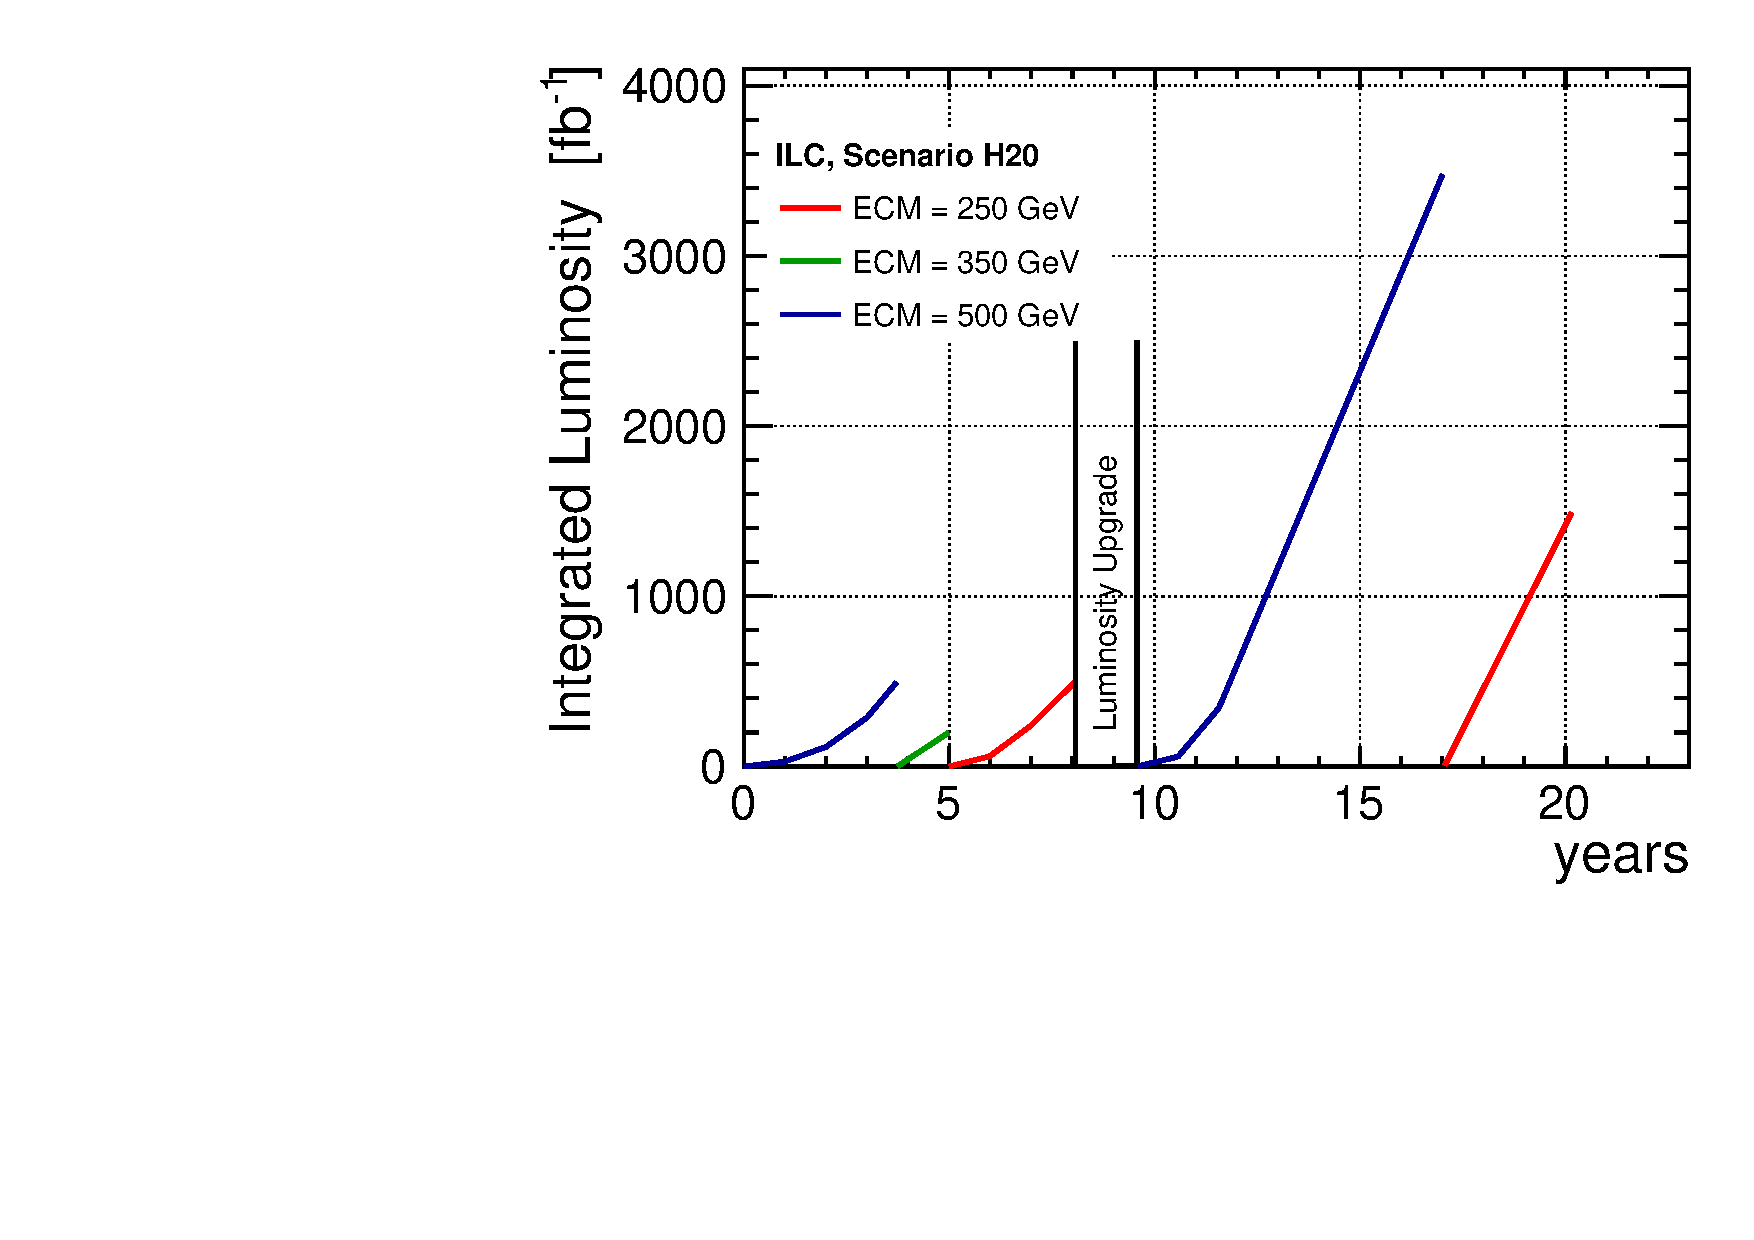
\includegraphics[width=0.85\hsize]{chapters/figures/lumi_H20.pdf}
\end{center}
\caption{The nominal 20-year running program for the 500-GeV ILC~\cite{Barklow:2015tja}.}
\label{fig:H20}
\end{figure}
%%%%%%%%%%%%%%%%%%%%%%%%%%%%%%%%%%%%%%%%%%%%%%%%%%%%%%%%%%%%%%%%%%%%%%%%%%%

After this general-purpose survey at the maximum energy, it was planned to collect dedicated datasets at lower energies, at the $t\bar{t}$ production threshold, for a precision determination of a theoretically well-defined top mass, and somewhat above the $ZH$ production threshold, near the maximum of the cross section.  The $ZH$ measurements at 250\,GeV would be a very important component of the program  even under the assumption that energies of  500\,GeV are immediately available.  This is true for two reasons.  First, in Higgsstrahlung production, each Higgs boson  is tagged by the recoil $Z$.  There are many measurements that 
rely on this tag to identify Higgs bosons or to measure absolute rates without the need to make assumptions about the Higgs decay modes.  These include the
the measurement of the normalized total cross section for the Higgsstrahlung process, the measurement  of  absolute branching ratios of the Higgs boson and the search for invisible and exotic decays.  At 500\,GeV, far above the threshold, recoil measurements become less characteristic, due to the more substantial ISR and increased amount of beamstrahlung with respect to \ 250\,GeV, and are subject to additional backgrounds.   Other measurements depend on precise reconstruction of the kinematics of the $\ee\to ZH$ process.
For example, the ultimate precision on 
the Higgs mass will be obtained using the kinematics of $Z$ recoil.  The search for deviations from the SM predictions for 
 Higgs decays requires as input a very precise value of this mass; see Sec.~\ref{sec:higgs:sigmazh}.
Another reaction that depends crucially on precise kinematic measurements is the $CP$ analysis of the $H \to \tau^+ \tau^-$ decay, discussed in Sec.~\ref{subsubsec:higgstautauCP}.

For a 500\,GeV machine running at 250\,GeV, the luminosity can be straightforwardly increased by a factor of 2 from the TDR value 
by the increase of the repetition rate for bunch trains  from 5 to 10\,Hz.  This improvement was incorporated in the plan H20 shown in Fig.~\ref{fig:H20}  even
at the initial stage of 250\,GeV running.

The H20 plan also included provision for an additional luminosity upgrade by doubling the number of bunches in each bunch 
train. This upgrade requires machine improvements as described in Sec.~\ref{subsubsec:upg-optL}, and after these improvements all further 
data would be taken in this mode.
This would give a total  4\,ab$^{-1}$ data sample at 500\,GeV.   A sample of this size is required for meaningful precisions on the top Yukawa coupling and on the Higgs self-coupling. These measurements remain by far statistically limited and  thus would profit from any further increase of the luminosity. In case of the top Yukawa coupling, it was noted that it is absolutely crucial to reach 500\,GeV, since already at 490\,GeV, thus when falling short of the target energy by only 2\%, the precision of the measurement would worsen by nearly a factor of 2. On the other hand, a moderate increase of the center-of-mass energy by 6\% to 530\,GeV would improve the precision on the top-Yukawa coupling by a factor of 2. This should be considered in the planning of the energy upgrade of an inital 250\,GeV machine, see also discussion in Sec.~\ref{subsubsec:upg-optE}.

Finally the H20 scenario planned a run at 250\,GeV, now with 4 times the TDR luminosity, to finish the collection of a 2\,ab$^{-1}$ data set.   This run would provide the ultimate precision on the Higgs boson mass and the total $ZH$ cross section. It should be stressed again that the current focus on three fixed center-of-mass energies does not preclude running at any other desired intermediate energy, \eg\ for scanning the production threshold of newly discovered particles.

At the end of this 20 year program, we envision  a further doubling of the energy to 1\,TeV.   This upgrade was presented already 
in the ILC TDR and is reviewed in Sec.~\ref{subsubsec:upg-optE}.  This energy upgrade could  possibly be preceeded by a run at the $Z$ pole if it is  required by the  physics.

%\ref{sec:design_evo}
\subsubsection{Running Scenarios for the Staged Machine}

With the introduction of the staging plan for the ILC machine construction, it was necessary to change the time ordering of the 
various energy steps in the program described in the previous subsection. However, the total integrated luminosities to be collected at each center-of-mass energy, which were already optimized for the physics goals,  were left untouched. Thus,  all physics projections based on the H20 scenario remained valid - albeit the results will arrive in a different time order. Figure~\ref{fig:H20staged-orig} shows the original plan for the time evolution of the staged H20 scenario. The assumptions differ from those listed in the previous subsection in the following points:
\begin{itemize} 
\item No 10\,Hz operation is assumed since in the 250\,GeV machine the cryomodules will be operated at full gradient and thus no spare cryo- and RF-power is available. Technically, it would be possible to increase the repetition rate (and thus the luminosity) at any time provided that resources for installing the additional cryo- and RF-power and for covering the higher operation costs could be found. This option is {\em not} included in the staging scenario.
\item The luminosity upgrade by doubling the number of bunches per train (c.f.\ Sec.~\ref{subsubsec:upg-optL}) is a smaller investment than the energy upgrade and will therefore happen first. In this plan, the second positron damping ring and the additional cryo- and RF-power needed for the luminosity doubling would  already be installed at the start of 500\,GeV operation.  Then the entire 500\,GeV run would be done at 2 times the TDR luminosity. 
\item The energy upgrade (described in\ Sec.~\ref{subsubsec:upg-optE}) requires only a relatively short machine shutdown of about one year, since major parts of the new tunnel can be constructed and the new parts of the machine can be installed without disturbing the operation of the 250-GeV machine. A shutdown is necessary only during the construction of the connections of the new parts of the  machine to the older ones.
\item After the energy upgrade the same ramp fractions as for a completely new machine are assumed, thus 10\%, 30\%, 60\% and 100\% over the first four calendar years.
\end{itemize}
With these assumptions, the real-time for realization of  the full H20 program increases from 20 to 26 years, 
mostly due to the much longer time to collect the 2\,ab$^{-1}$ at 250\,GeV without 10\,Hz operation. 


%%%%%%%%%%%%%%%%%%%%%%%%%%%%%%%%%%%%%%%%%%%%%%%%%%%%%%%%%%%%%%%%%%%%%%%%%
\begin{figure}
\begin{center}
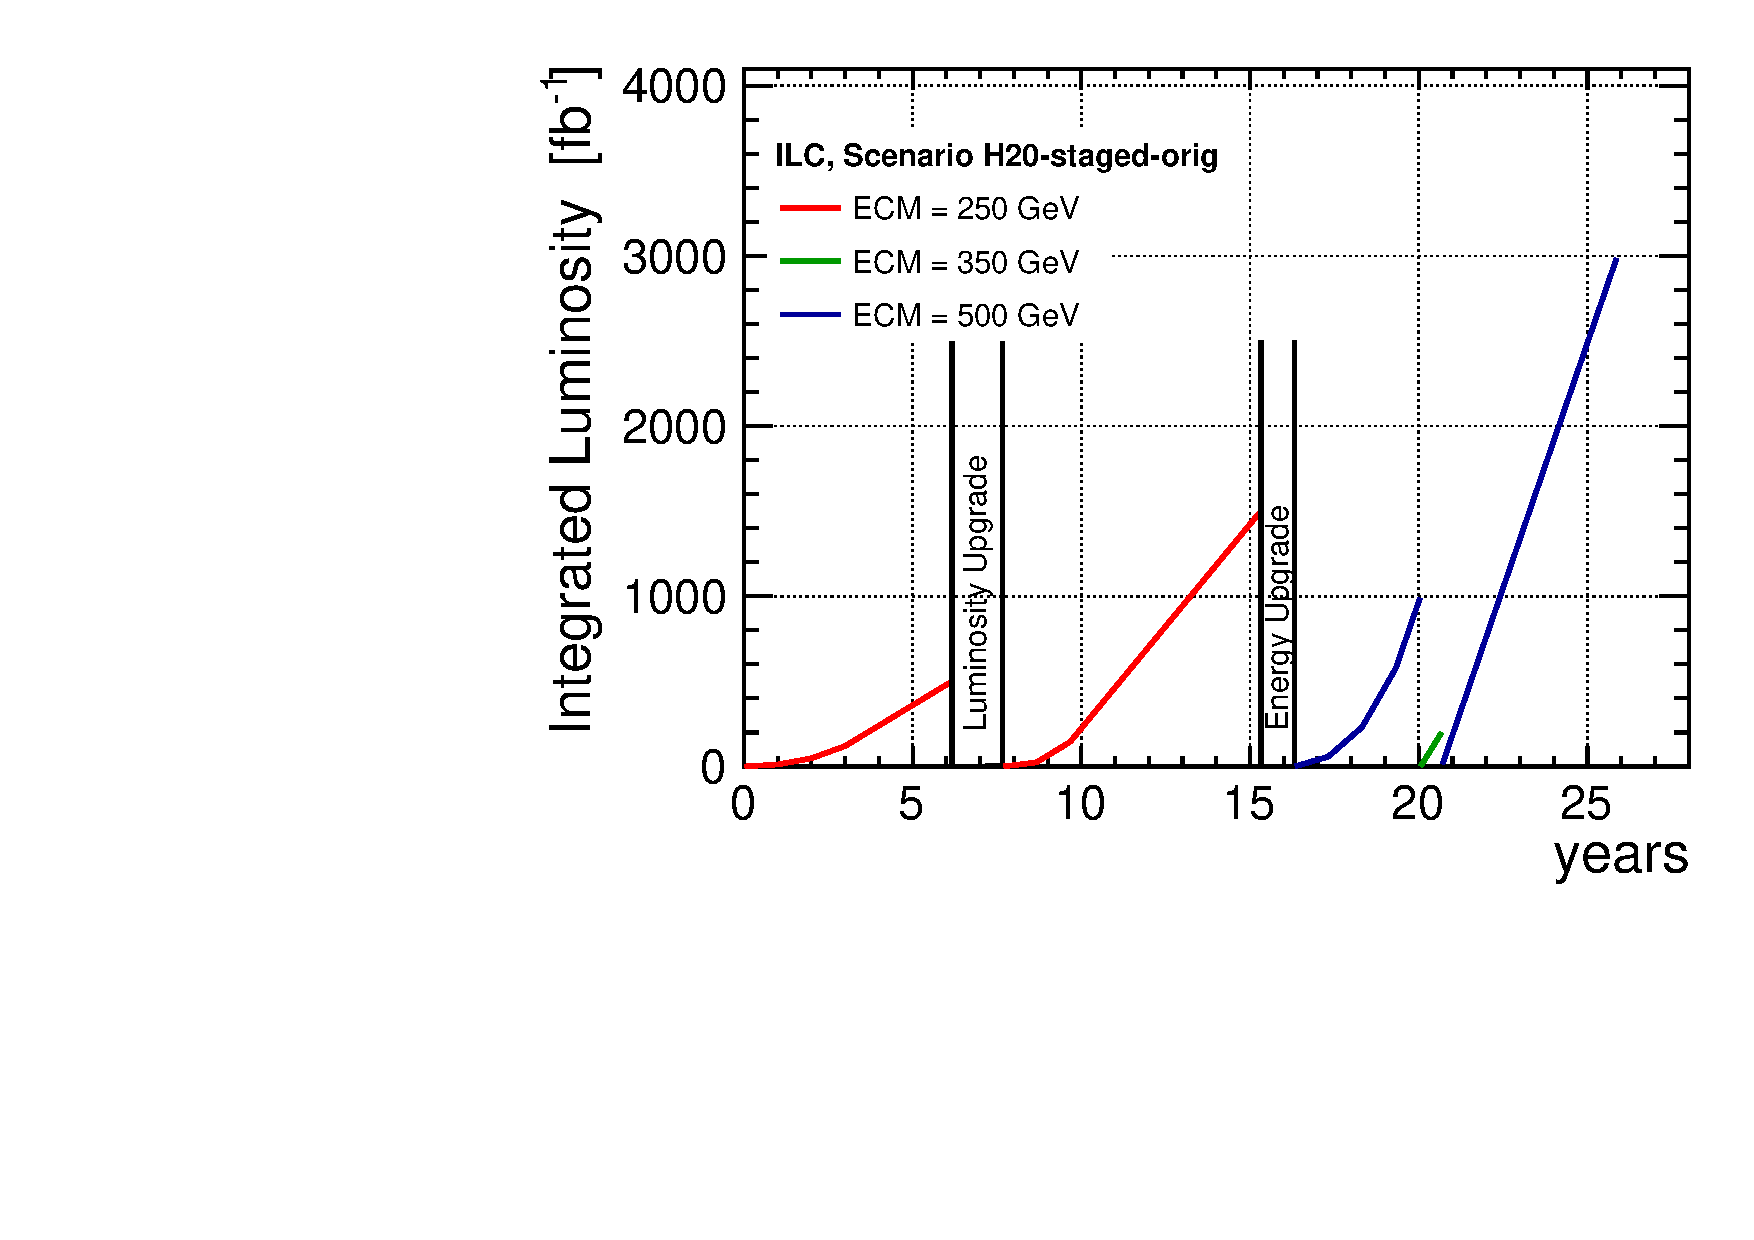
\includegraphics[width=0.85\hsize]{chapters/figures/lumi_H20-staged-orig}
\end{center}
\caption{The nominal 26-year running program for the staged ILC, starting operation at 250\,\GeV without the possibility to operate at 10\,Hz.~\cite{Fujii:2017vwa}. The integrated luminosities are the same of for the original H20 scenario.}
\label{fig:H20staged-orig}
\end{figure}
%%%%%%%%%%%%%%%%%%%%%%%%%%%%%%%%%%%%%%%%%%%%%%%%%%%%%%%%%%%%%%%%%%%%%%%%%%%

In order to mitigate the absence of the 10\,Hz operation, which would require additional investments beyond the minimal 250-GeV machine, cost neutral ways to increase the luminosity at 250\,GeV have been studied, as discussed in Sec.~\ref{sec:ilc}. In 2017, a new set of beam parameters for the 250-GeV ILC was officially adopted~\cite{bib:cr-0016}.  It is this parameter set that is shown in the column ``initial'' of Tab.~\ref{tab:ilc-params}. The 65\% increase in instantaneous luminosity w.r.t.\ the TDR parameters is achieved by reducing the horizontal emittance by a factor of 2. This leads to a larger luminosity in each bunch crossing and thus to an increase of beamstrahlung, background from $e^+e^-$ pairs and pile-up from low-$p_t$ $\gamma\gamma \to$\,hadrons events. Neither these effects, nor the slightly wider luminosity spectrum which results from the increased beamstrahlung are included in the physics case studies presented in the following sections, since no new Monte-Carlo samples could be produced (and analysed) since the new beam parameters became available. However, even with the new beam parameters the background conditions at 250\,GeV do not become worse than what is expected at 500\,GeV, a case already studied in detail.  The ILC detectors have actually been designed for high performance in the more difficult  beam conditions at 1\,TeV. Therefore, the impact of the new beam parameters on the majority of the physics anayses is expected to be minor. The analysis most strongly affected is the mass measurement of the Higgs boson via the leptonic recoil method, described in Sec.~\ref{sec:higgs:sigmazh}. For this analysis, the new beam parameters have been estimated to result in a relative degradation of the ultimate precision on the Higgs mass by about 25\%~\cite{bib:jeans_awlc17} compared to the same amount of total luminosity collected with the TDR beam parameters.  This still corresponds to an impressive 
Higgs mass measurement to better than 20\,MeV. 

We have already shown in Fig.~\ref{fig:H20staged} the default running scenario for the staged ILC based on the new beam parameters for 250\,GeV~\cite{bib:cr-0016}. Compared to Fig.~\ref{fig:H20staged-orig}, the total run time shortens from 26 years to 22 years, thus recovering about 2/3 of the original increase in running time. A full-scale Monte-Carlo production with the new beam parameters and based on the ILD detector concept is planned for 2019.


None of the running scenarios explicitly includes the option to increase the positron polarisation to 60\% when operating at a center-of-mass energy of 500\,GeV. Numerous studies~\cite{Fujii:2018mli, Habermehl:417605, Moortgat-Picka:2015yla, Aurand:2009kp, MoortgatPick:2005cw} have shown that all physics measurements will profit from the corresponding increases in effective luminosity and effective polarisation. In this respect, all physics projections for 500\,GeV are still quite conservative.

   
   
\section{\label{sec:physics}Physics Case (250 GeV) }

10 pages Peskin
 
% section on the physics case


The core of the physics case for the ILC is to make high-precision
 measurements of the properties of the Higgs boson.    The Higgs
 field is at the core of
 the SM.  It is responsible for the masses of all known
 elementary particles.
  It is also responsible for those aspects of the SM that are
 hardest to  understand----the
presence of spontaneous gauge symmetry breaking, the  hierarchy of quark and lepton masses, and the appearance of flavor mixing and $CP$ violation in weak 
interactions.
If we wish to learn more about these features of the fundamental laws of nature, an obvous course is to measure the Higgs boson as well as we are able.  We will argue in this section and the succeeding ones that ILC will be able to determine the mass of the Higgs boson to a part in $10^4$ and the major couplings of the Higgs boson to than 1\% accuracy.   This will qualitatively sharpen the picture of the Higgs boson that we will obtain even from the high-luminosity stage of the LHC. 

This set of measurements, and other measurements available for the first time at the ILC, will open new paths in the search for new fundamental interactions beyond the SM. 
Though the SM seems to account for all elementary particle phenomena observed up to now, it is manifestly incomplete.   It not only does not answer but actually is incapable of answering the questions posed in the previous paragraph.  It also cannot address basic facts about the universe in the large, in particular, the excess of matter over antimatter and the origin of the cosmic dark matter.  To make progress, we need observational evidence from particle physics of violations of the SM.  These will provide clues that can show the way forward.

Up to now, we have sought evidence for new interactions from direct searches for new particles at LEP, the Tevatron, and the LHC, from measurements of the $W$ and $Z$ bosons, and from searches for anomalies in flavor physics.  We are now approaching the limits of these techniques with current particle physics facilities.  The ILC will 
extend our search capabilities in precision measurements of $W$ boson couplings and fermion pair production, and will provide new opportunites for the direct discovery of new particles.  But, most of all, it will open a completely new road through the thorough, high-precision study of the Higgs boson. 


\subsection{Mysteries of the Higgs boson}

We often hear from our colleagues that the Higgs boson, as observed at the LHC, is an uninteresting particle, since it conforms so well to the expectations from the SM.   In fact, aside from our knowledge of the Higgs boson mass, the measurements make so far at the LHC tell us almost nothing about the true nature of this particle.   We now 
explain this statement, and, in the process, clarify the requirements for measurements of the Higgs boson couplings that can give insight into physics beyond the SM. 

New physics can correct the Higgs boson couplings in many ways.  However, in all cases, the size of the corrections is limited by the Decoupling Theorem, enunciated by Haber in \cite{Haber:1994mt}:    If the new particles that modify the SM have minimum mass $M$, then  the corrections to the SM predictions for the Higgs boson couplings are of size 
\beq 
              a \,     m_h^2 / M^2   \  .
\eeqn
where the coefficient $a$ is of order 1.   The exclusions of new particles through searches at the LHC suggest that $M$ is at least close to 1~TeV.   Then the effects of  new physics are limited to the few-percent level.   We will illustrate this result with explicit models in the next subsection.

The proof of the theorem is simple and illustrative.   It can be shown that the SM is actually the most general renomalizable quantum field theory with $SU(3)\times SU(2)\times U(1)$ gauge symmetry and the known particle content.   If we add new particles with masses of $M$ and above, we can assess their influence on the Higgs boson by integrating them out of the theory.  This adds to the Lagrangian a set of new terms with the SM symmetries.   The terms in the new Lagrangian  can be organized by their operator dimension 
as 
\beq 
   {\L}  =  {\L}_{SM} + {1\over M^2} \sum_i\,  c_i \O_{6i} + {1\over M^4 } \sum_j\,  d_j\O_{8j} + \cdots
\eeq{geneffL}
where $\L_{SM}$ is the SM Lagrangian with modified parameters, $\O_{6i}$  are operators of dimension 6, $\O_{8j}$ are operators of dimension 8, \etc.   The shifts in the SM parameters are not observable, since these parameters are in any case fit to experiment.  Then the leading observable corrections are of order $M^{-2}$. 

This theorem has a striking consequence.  Instead of a model with a single Higgs doublet, as we have in the SM, nature could be providing  a model with two or more Higgs fields, composite Higgs fields, even a whole Higgs sector.  All of this possible complexity is hidden from us by the Decoupling Theorem. 

The theorem has an appealing corollary, though.   Since the SM is the most general renormalizable model, once its parameters are known, its predictions for the Higgs couplings are determined precisely.   These predictions do depend on measured SM parameters such as $m_b$, $m_c$, and $\alpha_s$, but  it is argued in \cite{Lepage:2014fla} that  
lattice QCD will determine these well enough to fix the SM predictions for Higgs to part-per-mil accuracy.   Then, if we can observe corrections to the SM predictures at the 1\% level, these corrections and the evidence that they give for new physics cannot hide.

\subsection{Examples of  new physics influence on the Higgs boson}
\label{subsec:newphysicofH}

Many models of physics beyond the SM illustrate the points made in the previous section. Here are some examples.   These examples point to  a goal of 1\% accuracy
for the measurement of Higgs boson couplings in the major decay modes.

Models with two Higgs doublets contain 5 physical Higgs particles: two  neutral $CP$-even states $h$, $H$,  a neutral $CP$-odd state $A$, and a pair of charged scalars $H^\pm$.  These states are mixed by two angles $\alpha, \beta$. The lighter
$CP$-even state $h$ is identified with the observed Higgs boson.  Its couplings to 
fermions depend on the mixing angles.   For example, in the ``Type II'' case, 
\beq
   g(hb\bar b) = - {\sin\alpha\over \cos\beta}{m_b\over v}  \quad   g(hc\bar c) =  {\cos\alpha\over \sin\beta}{m_c\over v}   \ .
\eeqn{typeIIbcshift}
However, the mixing angles are connected to the masses in such a way that when the additional bosons become heavy, their effects in \leqn{typeIIbcshift} also become small,
\beq
     - {\sin\alpha\over \cos\beta} =  1 + \O({m_Z^2\over m_A^2}) \ .
\eeqn
conforming to the Decoupling Theorem.   In Type II models, the $b$ and $\tau$ Yukawa couplngs are shifted together by about 5\% for $m_A = 500$~GeV, and by decreasing amounts when all of the additional bosons become heavier.

%%%%%%%%%%%%%%%%%%%%%%%%%%%%%%%%%%%%%%%%%%%%%%%%%%%%%%%%
\begin{figure}
\begin{center}
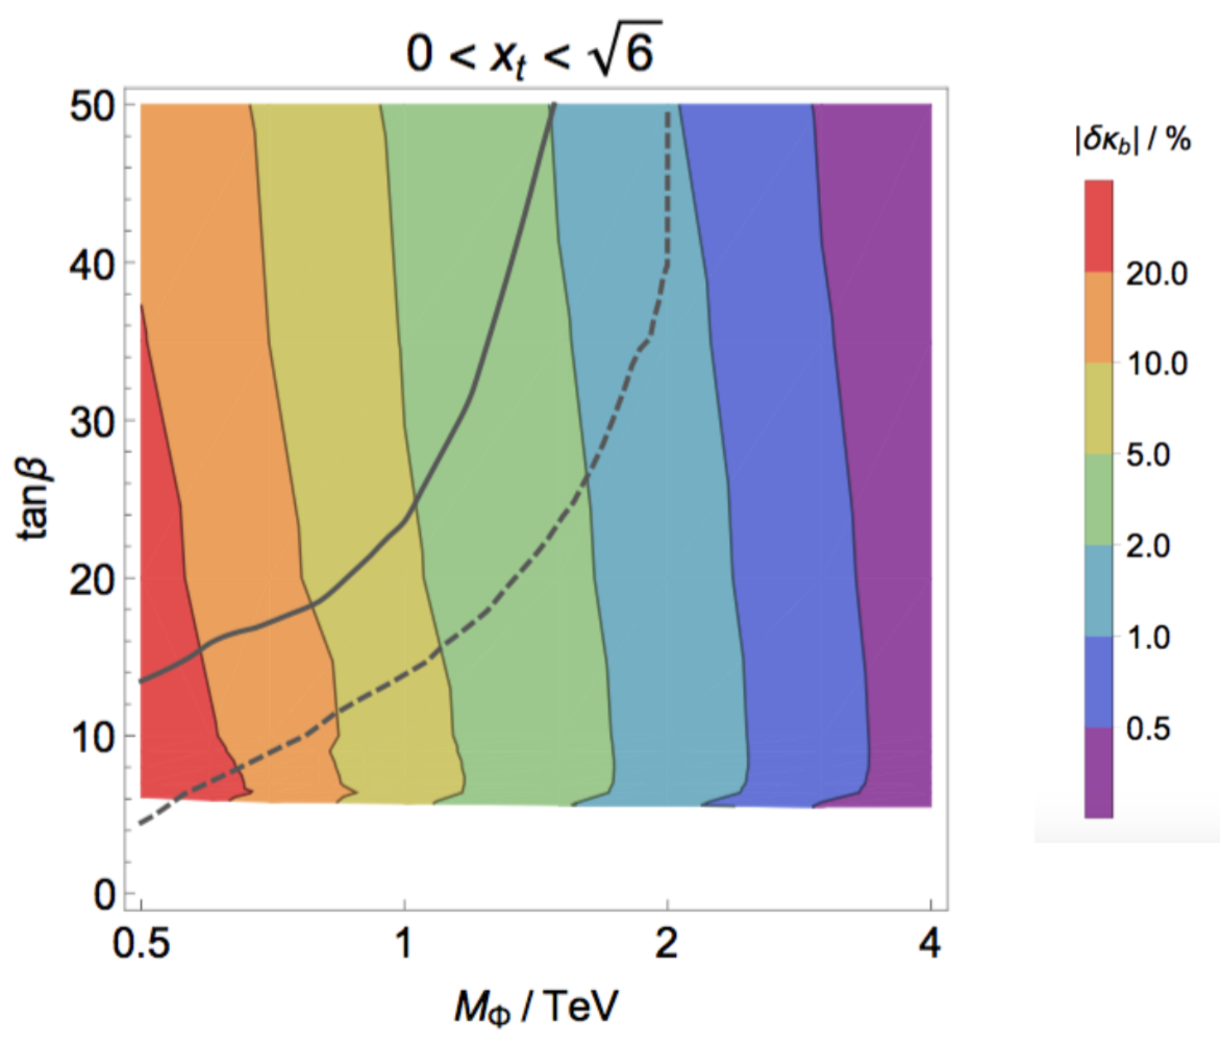
\includegraphics[width=0.90\hsize]{chapters/figures/WellsZhang.pdf}
\end{center}
\caption{Deviation from the SM prediction for the $hb\bar b$ 
coupling over a parameter space of grand-unified SUSY models, from \cite{Wells:2017vla}.   
Models in the upper left-hand corner are excluded by current LHC searches.  
Models above the dashed line are expected to be excluded at the  HL-LHC. 
The color-code indicates the magnitude of the coupling deviation, in \%. }
\label{fig:WellsZhang}
\end{figure}
%%%%%%%%%%%%%%%%%%%%%%%%%%%%%%%%%%%%%%%%%%%%%%%%%%%%%%%%%%%%%%


Supersymmetry (SUSY) models contain Type II  two-Higgs-double sectors, but they also contain other effects that modify the Higgs boson couplings.   Mixing between the scalar partners of $b_L$ and $b_R$ can generate a shift of the $hb\bar b$ coupling through loop diagrams.  The magnitude of this effect in 
grand-unified SUSY models is shown in 
Fig.~\ref{fig:WellsZhang}~\cite{Wells:2017vla}.   
Note that it is possible to have a large shift of the Higgs boson coupling for 
parameter values where the SUSY particles are too
heavy to be discovered at the LHC.   Thus, the search for shifts in the Higgs couplings away from the SM predictions provides a method of searching for this new physics that is indepedent of, and largely orthogonal to, the direct search for SUSY particles.   Other surveys of this effect in \cite{Cahill-Rowley:2014wba,Kanemura:2015mxa}  confirm this idea.

SUSY models typically predict very small shifts of the $hWW$ and $hZZ$ couplings, but other types of models can affect these couplings directly.   Models in which the electroweak phase transition becomes first-order and allows baryogenesis at the weak scale often involve mixing of the Higgs field with a heavy singlet field.  This gives
\beq
           g(hWW) = {2m_W^2\over v} \cos^2\phi\approx  {2m_W^2\over v} (1 -\half \phi^2) \ ,
\eeqn{scalarmixing}
where $\phi \sim  m_h/m_S$, and similarly for the $hZZ$ coupling~\cite{Hscalarmixing}   In composite models of the Higgs
 field, the Higgs field often appears as a Goldstone boson of a new strong interaction theory, giving a coupling modification by $(1- v^2/f^2)^{1/2}$, where $f$ is the Goldstone boson decay constant~\cite{HiggsasGB}.  This effect is similar to that in \leqn{scalarmixing}.

Models of Higgs compositeness, ``Little Higgs'' models, and models with extra space dimensions all contain new heavy vectorlike fermions $T$.   Typically, these fermions obtain a fraction of their mass from the Higgs mechanism (perhaps by mixing with the top quark) that is of order $m_t^2/m_T^2$.   Then they induce corrections of this order to the loop-generated Higgs couplings $g(hgg)$ and $g(h\gamma\gamma)$.  Corrections as large as 10\% can be generated in specific models~\cite{Han:2003gf}.   These same mixing and compositeness effects modify the $ht\bar t$ coupling~\cite{Agashe:2004rs}.

An interesting picture emerges.   Almost all models of new physics generate corrections to the Higgs boson couplings.   Almost always, these corrections are small, below the 10\% level, in accord with the Decoupling Theorem.  However, in precision experiments that make these coupling deviations  visible, each type of new physics affects the Higgs couplings in different ways.  In general,
\begin{itemize}
\item The $hb\bar b$ and $h\tau\tau$ couplings are sensitive to models with additional Higgs doublets.
\item The $hb\bar b$ coupling is sensitive to heavy SUSY particles with left-right mixing.
\item The $hWW$ and $hZZ$ couplings are sensitive to mixing of the Higgs field with singlet fields, and to composite structure of the Higgs boson.
\item The $hgg$ and $h\gamma\gamma$ are sensitive to models with new vectorlike fermions.
\item The $ht\bar t$ coupling is sensitive to models with composite Higgs bosons and top quarks.
\end{itemize}

In each new physics model, the  deviations from the SM predictions for the Higgs couplings form a pattern.  With precision experiments, it is possible not only to discover the existence of new physics but also to read the pattern and gain clues as to the way forward.   A worked example of such model discrimination at the level of precision expected at the ILC  is presented in
Section~7 of  \cite{Barklow:2017suo}.


\subsection{Limitations of the LHC measurements on the Higgs boson}

Today, the LHC experiments are achieving 20\% uncertainties in their measurements of Higgs boson couplings.   Over the lifetime of the LHC, including its high-luminosity stage, these experiments will acquire a factor of 30 more data.   Shouldn't this lead to Higgs coupling measurements of the required high precision?  We believe that the answer to this question is no.   We give a high-level argument here. A detailed comparison of the expected ILC capabilities with those of the high-luminosity LHC will be presented in Sec.~\ref{subsec:higgs:ilclhc}.

We find three points relevant to this comparison.  First, the measurement of Higgs boson 
decays at the LHC is extremely challenging because of the difficulty of distinguishing 
signal from background.
In the two decay modes in which the Higgs boson was discovered, $h\to \gamma\gamma$ and $h\to 4\ell$, Higgs events are apparent, because all products of the Higgs are observed and the Higgs mass can be reconstructed with high accuracy.  Unfortunately, these modes correspond to tiny branching ratios,  0.2\% and and 0.02\% of Higgs decays, respectively.  For more typical decay  modes, Higgs boson decay events have no obvious differences in appearance from SM background reactions with larger rates.   For example, $h\to WW\to e\nu \mu \nu $ events differ from $q\bar q\to WW \to  e\nu \mu \nu $ events only in subtle features of the lepton momentum distributions.  To discover the Higgs boson in one of the major channels, the LHC experiments start from samples that are 10:1 background to signal (for $h\to b\bar b$, the ratio is 20:1). They then  extract the signal by significant kinematic cuts and the use of machine-learning classifiers.  It is already a triumph that ATLAS and CMS have been able to obtain significant observations. 

Measuring  the Higgs couplings with high precision is even more of a challenge.   It is currently beyond the state of the art to determine the efficiency  with which SM background events pass the cuts of a Higgs analysis to 1\% accuracy.   These background events must be subtracted from the Higgs signal, and so this 1\% would translate to a 10\% accuracy on the Higgs $\sigma\times BR$ or a 5\% error on the coupling. To go beyond this level is truly daunting.  Nevertheless, the studies reported in the HL-LHC Yellow Book~\cite{xxx} give reasons for optimism and cite goals of 2-4\%  for Higgs coupling uncertainties.

This brings us to the secoind point.  As we have emphasized already, the modifications of the Higgs boson couplings from new  physics are expected to be small.  In the previous section, we have argued that new physics interactions are expected to affect specific
Higgs boson couplings at a level of order 5\% or smaller.  A 2\% measurement of such a coupling  
would not meet the $3\sigma$ criterion for positive evidence of new physics.

Finally, one must take into account that the HL-LHC measurements will ultimately be limited by the systematic understanding of backgrounds  An deviation in Higgs couplings observed at the LHC is then likely to be questioned (as, for example, the $t\bar t$ forward-backward asymmetry from the Tevatron was) without a clear means of confirming the result. 
One sometimes hears that the LHC can measure ratios of branching ratios with improved accuracy, but this statement is wrong for the major modes, since each mode has different backgrounds and requires its own dedicated analysis. 

 In contrast, as we will argue below, the observation of Higgs coupling deviations at the ILC at  250~GeV would be statistics-limited and can be confirmed by experiments at 500~GeV that bring in a new production reaction with an independent, data set. 


\subsection{$\ee\to Zh$}

The arguments just presented call out for a different way to measure Higgs boson couplings.   In this method, Higgs boson events should be apparent with a simple discriminator that can then be refined for high-accuracy $\sigma\times BR$.  Ideally, this method should identify Higgs boson events independently of the decay mode, allowing the measurement of the total cross section for Higgs production and the discovery of exotic and unanticipated Higgs decays.

This new method will be provided by the ILC.  It is the measurement of the reaction $\ee\to Zh$ at 250~GeV.   At an $\ee$ collider at this energy, it is true to a first approximation that any $Z$ boson observed with a lab energy of  110~GeV is recoiling against a Higgs boson.   The backgrounds to this signature (present at about 30\% of the signal level before cuts)  come from radiative $\ee\to Z\gamma$ and $\ee\to ZZ$, reactions that are well-understood and computed from electroweak theory at the 0.1\% level. 

The reaction $\ee\to Zh$ provides {\it tagged} Higgs decays.   Thus, events can be selected independently of the Higgs decay mode.  Then (1) the  total cross section for this reaction can be measured, giving a means of absolutely normalizing Higgs boson couplings; (2)  Higgs branching ratios can be measured  by counting, independently of the production cross section; and, (3)  exotic decay modes of the Higgs boson can be observed as products recoiling against the $Z$ tag.   Some event displays, from full 
simulation, are shown in Fig.~\ref{fig:HiggsEvents}. 

%%%%%%%%%%%%%%%%%%%%%%%%%%%%%%%%%%%%%%%%%%%%%%%%%%%%%%%%
\begin{figure}
\begin{center}
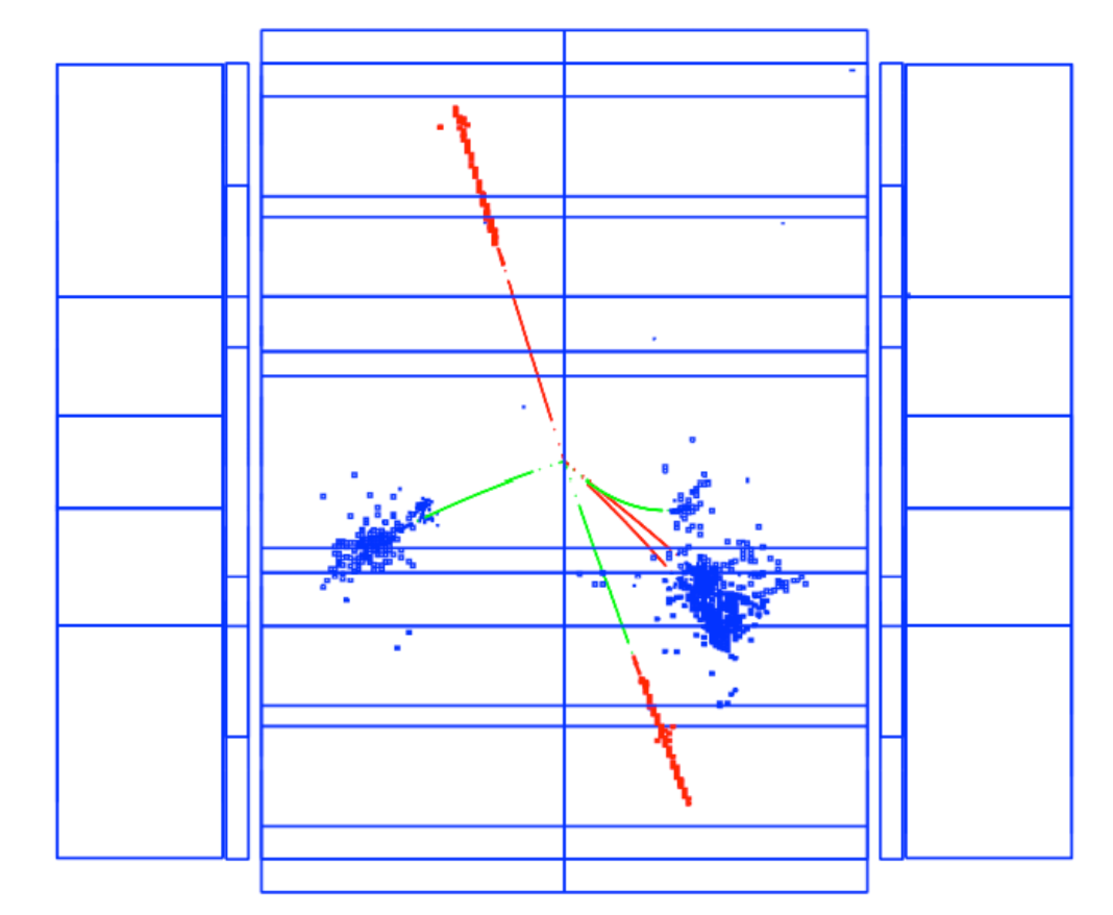
\includegraphics[width=0.5\hsize]{chapters/figures/htotautau.pdf}\ \ 
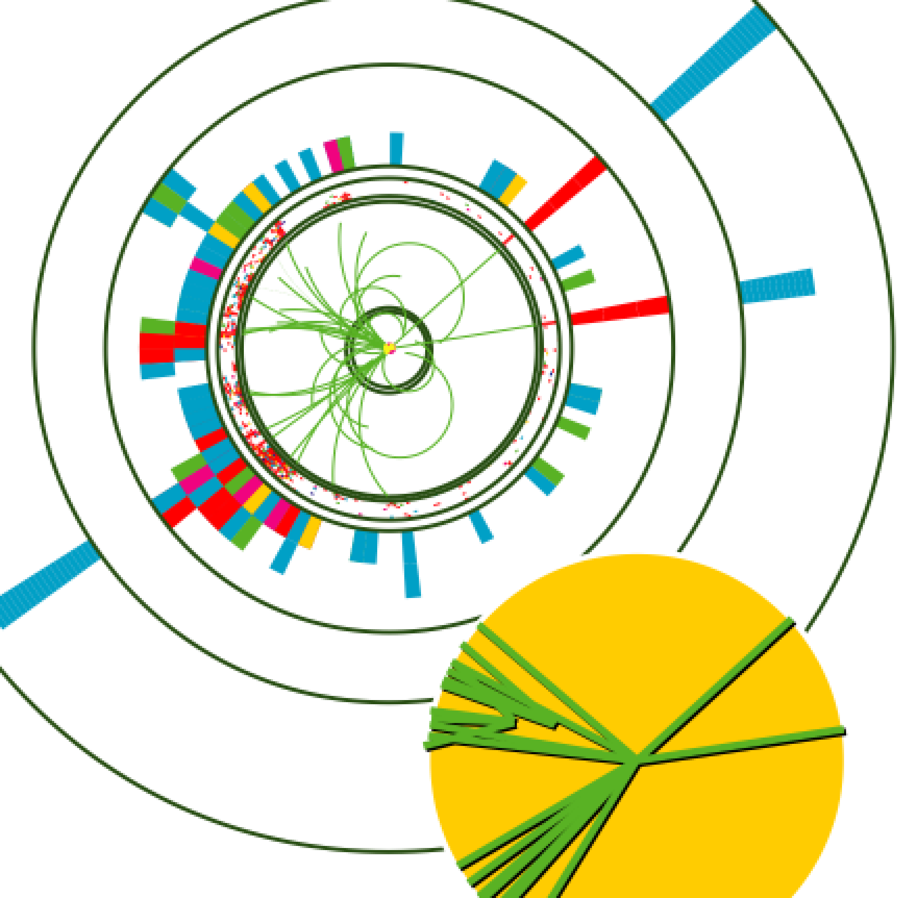
\includegraphics[width=0.40\hsize]{chapters/figures/htobb.pdf}
\end{center}
\caption{Event displays of $\ee\to Zh$ events  with $Z\to \mu^+\mu^-$, from full simulation: Left: $h\to \tau^+\tau^-$, ILC detector model;  Right: $h\to b\bar b$, SiD detector model.}
\label{fig:HiggsEvents}
\end{figure}
%%%%%%%%%%%%%%%%%%%%%%%%%%%%%%%%%%%%%%%%%%%%%%%%%%%%%%%%%%%%%%

\subsection{Search for exotic Higgs decays}

The fact that the reaction $\ee\to Zh$ yields {\it tagged} Higgs decays opens the 
possibility of another type of search for new physics.
The Higgs field is unique among SM fields in that it can form a dimension-2 operator 
$\Phi^\dagger \Phi$ with zero SM quantum numbers.  If there is any sector of fields that contains its own scalar field $\Sigma$, there will in general be a renormalizable coupling 
\beq
          \Delta \L   =   \eta\    (\Phi^\dagger \Phi) \, (\Sigma^\dagger \Sigma)  \ .
\eeq{Higgsportal}
The coupling constant $\eta$ is dimensionless, so the connection can be made at any (high) mass scale.   Thus it is possible for the Higgs boson to access a sector of elementary particles that have no other connection to the fields of the SM. 

If there is a new sector of particles with zero SM quantum numbers such that some of those particles have pair-production thresholds below 125 GeV, those particles should appear in Higgs boson decays.   If the particle that makes up cosmic dark matter is light enough to be produced in this way, the Higgs boson will have decays to invisible final states.   It is also possible that the new particles are unstable with respect to decay back to SM models.   A variety of scenarios are possible here, including decays to $4b$,
$4\tau$, $b\bar b$ + invisible states, and exotic particles with long lifetimes~\cite{Curtin:2013fra}.   With the data sample of the 250~GeV ILC, it is possible to search for all of these possible decay modes.   For  invisible Higgs decays, the expected 95\% CL exclusion limit on the  branching ratio is  $3\times 10^{-3}$, 
and for 
visible or partially visible modes the limits are in the range $10^{-3}$--$10^{-4}$~\cite{Liu:2016zki}. 

\subsection{Effective Field Theory framework for Higgs coupling determinations}
\label{subsec:phys_eft}

Though the goals of measuring the SM and exotic branching ratios of the Higgs boson are already very important, experiments at the ILC allow a further step.   The theory predictions described in Sec.~\ref{subsec:newphysicofH} refer to absolute partial decay widths.   These are 
related to the Higgs branching ratios by 
\beq
           \Gamma(h\to A\bar A) =   \Gamma_{tot} \cdot BR(h\to A\bar A)  \  .
\eeqn
The Higgs boson total width is very small---4~MeV in the SM---and it is not expected that any proposed collider can measure this value directly  with percent-level precision.
However, as we will now show, the ILC can determine the total width of the Higgs in a 
way that is highly model-independent and allows a 1\% absolute normalization of Higgs coupling constants.

A possible method to determine the Higgs width is to multiply each $hAA$ coupling by a parameter $\kappa_A$, and then fit these prarameters using data from $\ee\to ZH$.   In this simple method, the total cross section for $\ee\to ZH$ is proportional to $\kappa_Z^2$ and so the $\kappa_A$ parameters can be absolutely normalized.   This method has been used in much of the literature on Higgs coupling determinations, including \cite{Fujii:2015jha}.  In that paper, invisible and visible but exotic decay modes were treated by including these two partial widths as two additional parameters in the fit.  Using as inputs the measureable $\sigma\times BR$s for SM Higgs decay channels and Higgs decays to invisible final states, plus the total cross section for $\ee\to Zh$,  the ILC data would give a well-defined fit to the $\kappa_A$ parameters.

There are two problems with this method.  First, it is not completely model-independent.  Modelling the effects of new physics as a general set of dimension-6 operators as in \leqn{geneffL}, we find two different Lorentz structures for the modifications of the $hZZ$ vertex,
\beq
   \Delta \L =    (1 + \eta_Z) {m_Z^2\over v}  h Z_\mu Z^\mu + \zeta_Z {1\over 2v} h
   Z_{\mu\nu} Z^{\mu\nu} \ ,
\eeq{etazeta}
and a similar pair of structures for the $HWW$ vertex.  In principle, the two coefficients  in each case should be independently determined from data.  Second, the method does not make the most effective use of the data set from $\ee$ colliders.  The total width of the Higgs boson is determined from the ratio  $\sigma(\ee\to ZH)/\Gamma(H\to ZZ^*)$.  Since the denominator is a 3\% branching ratio, this strategy sacrifices a factor 30 in 
statistics.

A much more effective method for fitting Higgs boson couplings is described in \cite{Barklow:2017suo}.   In this method, we model the effects of new physics by the most general set of dimension-6 operators that can appear in \leqn{geneffL}.  The complete set of $SU(3)\times SU(2)\times U(1)$-invariant lepton- and baryon-number conserving dimension-6 operators  includes 59 terms~\cite{Grzadkowski:2010es}.  However, for 
the analysis of $\ee$ collider data, we can restrict ourselves to electron reactions 
producing the Higgs boson and other color-singlet states.  Since there is a single SM effective
 Lagrangian that should apply to all processes, this method allows us to combine data on 
Higgs production with additional data sets from $\ee\to W^+W^-$ and precision electroweak
measurements.   It is also possible to make use of additional observables for Higgs production
beyond simple rates.  In particular, the angular distribution and polarization asymmetry in 
$\ee\to ZH$ play important roles.  These considerations give the method based on 
Effective Field Theory much more power in extracting the most accurate estimates 
of the 
Higgs boson couplings from the data.

It is sometimes considered a restriction that the EFT model contains only operators of dimension 6 without considering operators of dimension 8 and higher.    This means that the model will be somewhat inaccurate for the effects of new particles of mass close to 125~GeV.  However, one should remember that the effects of the top quark and the Higgs boson on precision electroweak observables are well-modeled by the $S$ and $T$ parameters~\cite{Peskin:1990zt}---which are induced at the level of the dimension-6 EFT---even though the masses of these particles are not far above the $Z$ mass.   Very light new particles can have a different effect, providing new Higgs decay channels and giving additional contributions to the Higgs width.  We take these possible effects into account explicitly in our global fit, as we will explain in Sec.~\ref{subsec:global:elements}.

After we describe the experimental methods and the expected measurement uncertainties for Higgs production in  Sec.~\ref{sec:higgs} and for $W$ pair production in Sec.~\ref{sec:ew},  we will present formal  projections for uncertainties in 
Higgs couplings in Sec.\ref{sec:global}, making use of the EFT  method.  Suffice it to say that the data set expected for the ILC at 250~GeV is expected to measure the $hb\bar b$ couplings to 1\% accuracy, the $hWW$ and $hZZ$ couplings to better than 0.7\%, and the other 
major SM Higgs couplings to accuracies close to 1\%.    These measurements should be 
statistics-limited.  Above 250~GeV, a second Higgs production reaction, $\ee\to \nu\bar\nu h$ through $W$ boson fusion becomes important.  Using the additional data on $\ee\to Zh$ and the independent measurements from the $W$ fusion reaction, we expect that the uncertainties on Higgs couplings will decrease by another factor of 2. 


\subsection{$\ee \to W^+W^-$}
\label{subsec:phys_WW}
The reaction $\ee\to W^+W^-$ contributes to the analysis just described, but it has its own independent interest.  It has been appreciated for  a long time that this reaction provides an excellent way to test for the presence of dimension-6 operators that involve the $W$ and $Z$ fields.   The Feynman diagrams contributing to the reaction are shown in Fig.~\ref{fig:eeWWdiagrams}.   The process involves interference between $s$-channel diagrams with $\gamma$ and $Z$ exchanges and a $t$-channel diagram with neutrino exchange.  In the SM, there are large cancellations among these diagrams, but these are not respected by the dimension-6 contributions.   Thus, the dimension-6 coefficients appear in the cross section formulae enhanced by a factor $s/m_W^2$. 

%%%%%%%%%%%%%%%%%%%%%%%%%%%%%%%%%%%%%%%%%%%%%%%%%%%%%%%
\begin{figure}
\begin{center}
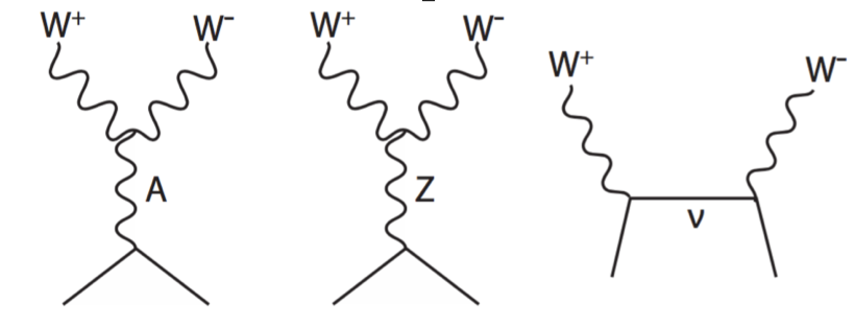
\includegraphics[width=0.80\hsize]{chapters/figures/WWdiagrams.pdf}
\end{center}
\caption{Feynman diagrams contributing to the process $\ee\to W^+W^-$ when contributing  dimension-6 operators are included.}
\label{fig:eeWWdiagrams}
\end{figure}
%%%%%%%%%%%%%%%%%%%%%%%%%%%%%%%%%%%%%%%%%%%%%%%%%%%%%%%%%%%%%%

The largest part of the dimension-6 effect can be described by shifts of the form 
factors for the $WW\gamma$ and $WWZ$ vertices.  These vertices can be parametrized as \cite{Hagiwara:1986vm}
\beq
\Delta \L = 
\eeq{WWgZvertex}
where $V = A,Z$.  In the SM, $g_{1A} = e$, $g_{1Z} = e s_w/c_w$ and the other coeficients are zero at the tree level.   The result $g_{1A} = e$ is exact due to the QED Ward identity.  The dimension-6 operator corrections generate a 3-parameter shift of the other 5 coefficients. These shifts can in principle be measured both at electron and at hadron colliders.  However, measurements in $\ee$ have  definite advantages.   First, it is possible to use final states with hadronic $W$ decays to determine the complete kinematics of each event and, using this information, to separate the production of 
transverse and longitudinal $W$ bosons.   Then, using beam polarization and $W$ final-state polarization, the 3 possible shifts of the form factors can be measured separately.   Second,  the greater intrinsic accuracy of measurements in $\ee$ give excellent results at a center of mass energies of 250--500~GeV.  At hadron colliders, 
the factor $s/m_W^2$ can be much larger, and one can take advantage of this by observing the reaction at $WW$ pair masses above 1~TeV.  However, this can lead to ambiguities due to the possible influence of dimension-8 operators, whose effects grow as $(s/m_W^2)^2$~\cite{Falkowski:2016cxu}. 

In Section VII  below, after describing the experimental study of $\ee\to W^+W^-$, we will show that the ILC at 250~GeV is expected to improve the precision of $W$ form factor measurements by an order of magnitude over expected results from HL-LHC.




\subsection{$\ee\to f\bar f$}
\label{subsec:phys_ff}

Fermion pair production provides a search for new forces that couple directly to the electron.   At LEP and LHC, $\ee$ and $q\bar q$ annihilation are used as probes for new gauge bosons appearing in the $s$-channel and for signals of fermion compositeness. 

The comparison with LEP 2 is instructive.   The ILC will operate at an energy not so far above that of LEP 2  (250~GeV {\it vs.}  180--208~GeV)  but with much higher luminosity (2 ab$^{-1}$  {\it vs.} a total of 1~fb$^{-1}$ over 4 experiments).   For statistics-limited measurements, this gives a factor 
\beq
   \biggl[{  s \cdot \int \L |_{ILC}\over s \cdot \int \L|_{LEP}} \biggr]^{1/2} \approx 
                    60 
\eeqn
improvement in sensitivity to deviations from the SM, or an improvement of  7.5 in the mass scale that can be accessed.   Though the comparison depends on the particular model, this corresponds to the ability to observed new vector bosons at 5--6 TeV and 
contact interaction scales of 70~TeV, comparable to  the projected reach of the HL-LHC. 

 In addition, the information from ILC is very specific.   Measuring the cross section for $\ee\to f\bar f$ in the forward and backward directions for $e^-_L$ and $e^-_R$ beams gives four  different observables, each of which corresponds to a different dimension-6 effective  interaction.   Discovery of an anomaly points directly to a model interpretation, either with an $s$-channel resonance or with new interactions at higher energy.   This information can be put together with results of resonance searches at the LHC. 

The reaction $\ee\to b\bar b$ deserves special consideration. In models in which the Higgs boson is composite, typically either the $t_L$ or the $t_R$ must be composite also to generate a large enough $t$ quark mass.    The $b_L$ is the $SU(2)$ partner of the $t_L$ and so must have the same admixture of composite structure.    If it is the $t_R$ that is more composite, it is not required that the $b_R$ is composite, but this often happens in models.  This can generate few-percent corrections to the rates for $e^-_{L,R} e^+\to b_R\bar b_L$ at the ILC.  ~\cite{Funatsu:2017nfm,YoonPeskin}.   It is possible that this effect, rather than effects in Higgs decays, would be the first indication of a composite Higgs sector. 

     
\subsection{Search for pair-production of new particles}

Despite the wide range of direct searches for new particle pair production at the LHC, 
those searches have blind spots corresponding to physically interesting models.  The two most important of these are:
\begin{enumerate}
\item  Insensitivity to new particles with electroweak interactions only that decay to an invisible partner with a mass gap of less than 5~GeV.   Though this case seems quite special, this is exactly the set of properties predicted for the charged Higgsino of SUSY models.  Dark matter scenarios involving coannihilation can also all into this blind spot, since in those models there is an electroweak partner separated from the dark matter particle by $k_B T$ at the thermal dark matter freezeout temperature of 5-10~GeV.
\item Insensitivity to production of pairs of invisible particles observed through radiation of an initial-state gluon.   At the LHC, such ``mono-gluon'' events have as a background initial state radiation in the Drell-Yan process, and the sensitivity to such events is limited by the precision of our knowledge of the Drell-Yan cross section.
\end{enumerate}
In both cases, the ILC can detect these new physics events for particle masses almost up to half of  the collider center of mass energy.

The experimental aspects of these particle seaches are discussed in Section~VIII.  A broader review of the opportunities for new particle discovery at $\ee$ colliders can be found in \cite{Fujii:2017ekh}.

\subsection{The central role of beam polarisation}
\label{subsec:beampol}

One theme that runs through all of the analyses discussed in the following Sections is the  important role of beam polarisation.   The use of beam polarisation may be unfamiliar to many readers, since all recently operated colliders -- the Tevatron, PEP-II and KEK-b, and the LHC -- have had unpolarised beams.   In hadronic 
collisions, the effects of polarisation are relatively small, first, because the dominant QCD interactions conserve parity and, second, because the proton is a composite particle, so high proton polarisation translates to much smaller polarisation for the constitutent quarks and gluons.   At a high-energy $\ee$ collider, the situation is very different.  The dominant interaction is the electroweak interaction, which has 
order-1 parity asymmetries in its couplings.  The beam particles are elementary, so that 80\% beam polarisation translates to 80\% polarisation in the colliding partons.
This implies  that polarisation effects are large at $\ee$  colliders and can be used to great advantage.   

It is very challenging to achieve high beam polarisation in circular colliders, especially for longitudinal polarisation.   Transverse beam polarisation was observed at LEP in single- and separated-beam operation but not for 
colliding beams~\cite{Assmann:1998qb}.  However,  a linear electron or positron
collider naturally preserves longitudinal beam polarisation.    The design of the 
ILC has been thought through  to produce, maintain, and control 
beam polarisation for both electrons and positrons, as has been explained in 
Sec.~\ref{par:beampol}.  This brings advantages for physics that we now discuss.

There are three major uses of beam polarisation in the experiments planned for ILC:
\begin{enumerate}
\item  Measurement of helicity-dependent electroweak couplings
\item Suppression of backgrounds and enhancement of signals
\item  Control of systematic uncertainties
\end{enumerate}
We discuss the first two of these points here.  The third, which is particularly 
important to claim a discovery from  precision measurements, is discussed in Sec.~\ref{subsec:polarization}.  A comprehensive review of the role of polarisation with many more examples can be found in~\cite{MoortgatPick:2005cw}, and, for  positron polarisation in particular, in~\cite{Fujii:2018mli}. 

To begin, we need some notation. Let $P_{e^-}$ and $P_{e^+}$ be, respectively, the longitudinal polarisations of the electron and positron colliding beams, equal to $+1$ for completely polarised right-handed beams and $-1$ for completely polarised left-handed beams.   Let $\sigma_{RR}$, $\sigma_{RL}$, $\sigma_{LR}$, $\sigma_{LL}$ be the cross sections for a given process completely polarised beams of the four possible orientations.  Since the electron has only two spin  states, the 
cross section for general beam  polarisations is given by 
\begin{eqnarray}
\sigma_{\Pem\Pep} &=& \frac{1}{4}\bigl\{
     (1+\Pem)(1+\Pep) \quad \sigmaRR  \nonumber \\
&& + (1-\Pem)(1-\Pep) \sigmaLL \nonumber \\
&& + (1+\Pem)(1-\Pep) \sigmaRL \nonumber \\ 
&& + (1-\Pem)(1+\Pep) \sigmaLR \bigr\},
\label{eq:pol:xsec}
\end{eqnarray}

For $s$-channel $\ee$ annihilation processes, helicity conservation implies that only $\sigma_{RL}$ and $\sigma_{LR}$ are nonzero.
In this case Eq.~\leqn{eq:pol:xsec} reduces to the simpler form
\begin{equation}
 \sigma_{\Pem\Pep} = 2 \sigma_0 (\Leff/\mathcal{L}) \left[1 - \ALR \Peff \right]
\label{eq:pol:xsecschan}
\end{equation}
where $\sigma_0$ is the unpolarised cross section, and \Leff\ and \Peff\  
are the effective luminosity and polarisation, defined, respectively, as 
\begin{equation}
\Peff= \frac{\Pem - \Pep}{1 - \Pep\Pem}
\label{eq:def-leff-peff}
\quad\mbox{\rm and }\quad
\Leff=\frac{1}{2}(1 -\Pep\Pem)\L \ . 
\end{equation}
The coefficient $\ALR$ is the intrinsic left-right asymmetry of the reaction cross section,
\beq
  \ALR =    {\sigmaLR - \sigmaRL\over \sigmaLR + \sigmaRL } \ . 
\eeq{eq:def-ALR}

In the electroweak interactions, it is typical that left-handed fermions have larger coupling constants than right-handed fermions.   Then, choosing $\Pem$ to be left-handed (negative) and $\Pep$ to be right-handed (positive) can confer important advantages.
Consider, for example, the typical ILC values $\Pem = -80\%$, $\Pep = +30\%$.    Then the effective polarization 
Eq. \leqn{eq:def-leff-peff} for the measurement of $\ALR$ values is  $\Peff = 90\%$.   The Higgsstrahlung process has a rather small polarisation asymmetry, $\ALR = 0.151$. Still, for the luminosity is enhanced from the unpolarised case by  $ 40\%$. 

Such substantial values of the beam polarisations can be applied to physics measurements in the following ways:
\begin{itemize}
\item In $\ee\to f\bar f$, the $e^-_L$ and $e^-_R$ couple to different linear combinations of the $s$-channel $\gamma$ and $Z$
propagators.  Beam polarisation allows us to measure the couplings to these vector bosons independently.  In addition, an $s$-dependent change in the polarisation asymmetry can signal the presence of a new $s$-channel resonance.  
\item Similarly, in $\ee\to W^+W^-$, the separation of $\gamma$ and $Z$ couplings can be combined with information from the $W$ production angle and polarisations to completely disentangle the 14 complex parameters (28 real parameters) in the most general 
Lagrangian for triple gauge vertices.
\item In $\ee\to ZH$, measurement of  the polarisation asymmetry plays an important role in disentangling the various of  parameters 
that enter the EFT analysis of Higgs boson couplings.
\item If new particles are discovered in pair-production at the ILC, measurement of the production cross section with different beam polarisation settings allows their electroweak quantum numbers to be determined unambiguously.
\end{itemize}
We will discuss all of the applications below.

%%%%%%%%%%%%%%%%%%%%%%%%%%%%%%%%%%%%%%%%%%%%%%%%%%%%%%%%%%%%%%%%%%%%%%%
\begin{figure}
\centering
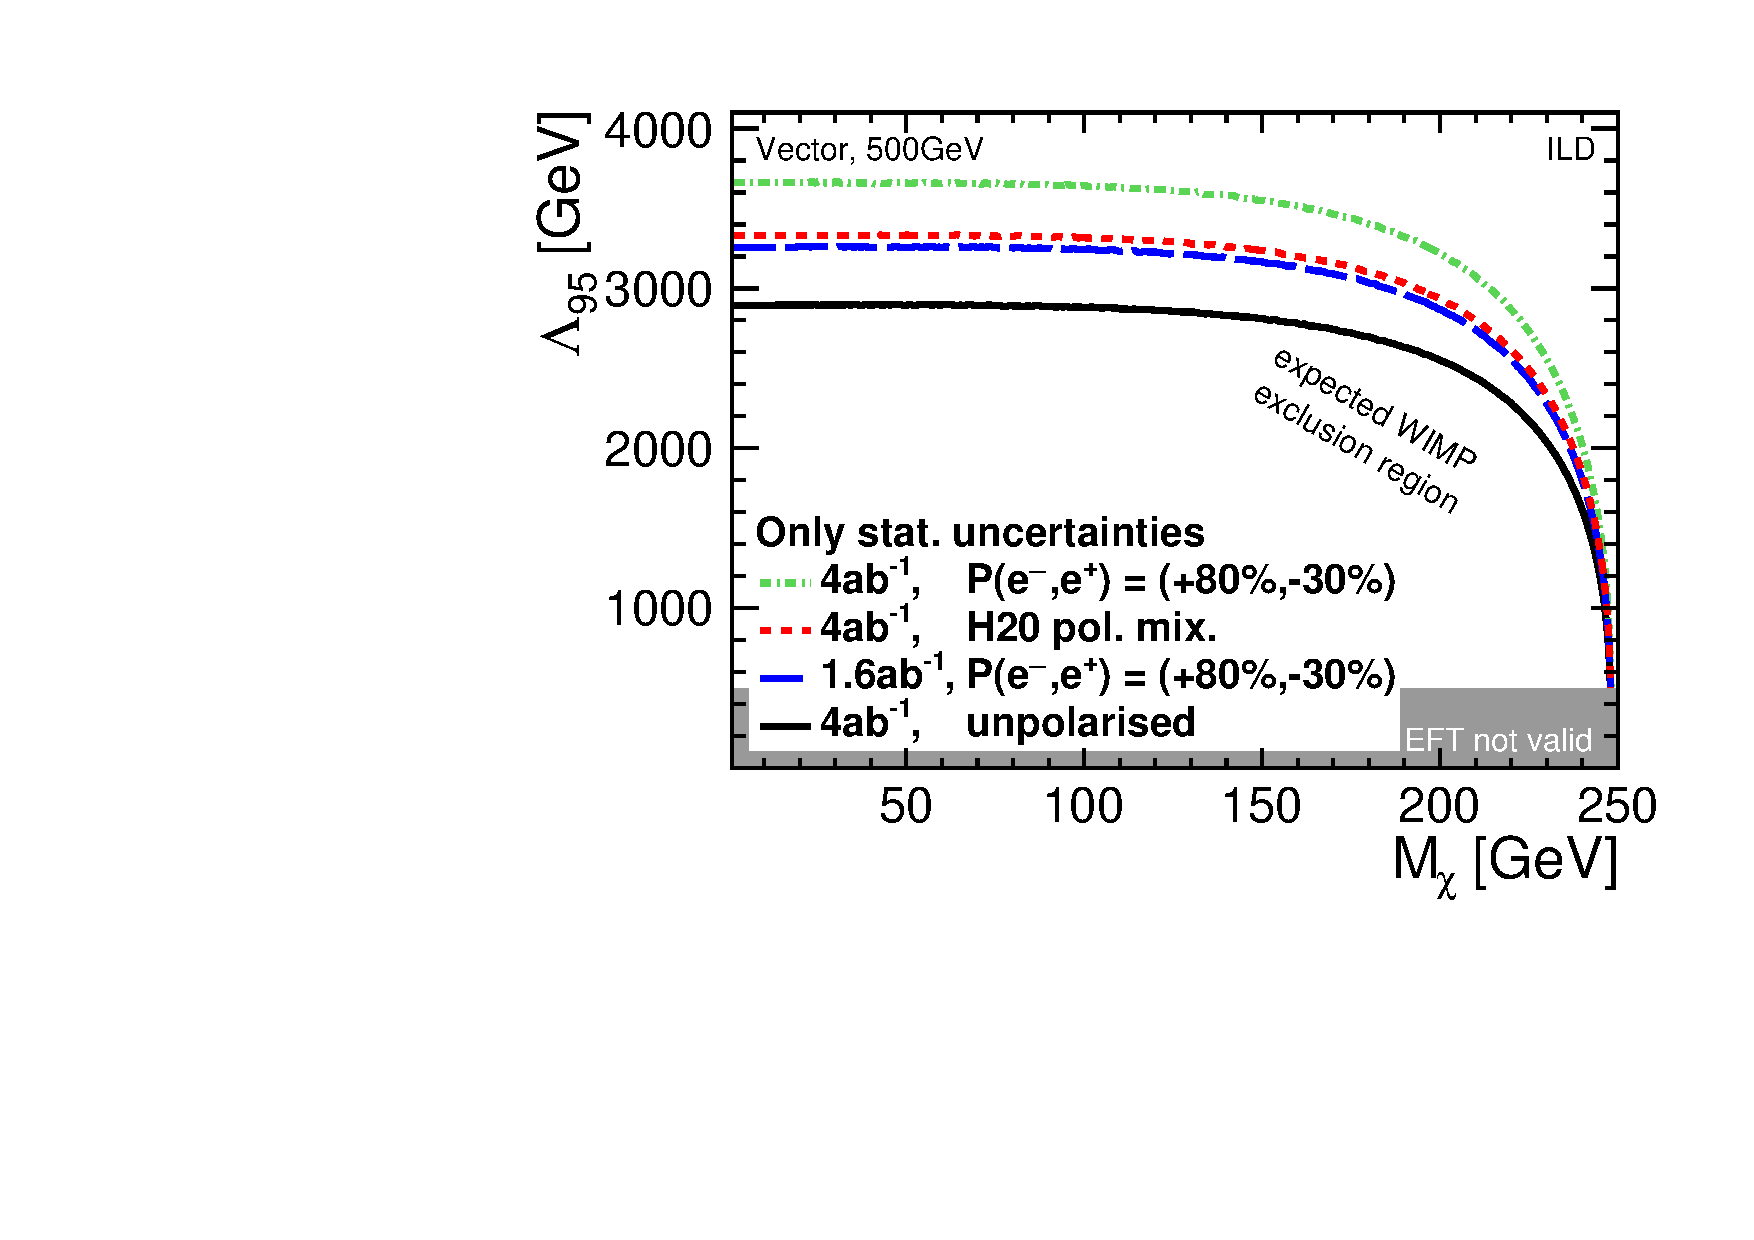
\includegraphics[width=0.95\linewidth]{./chapters/figures/vector_noSystematics.pdf}
		
\caption{Comparison of the 95\% confidence lower limit on the mediator scale for dark matter production using  the mono-photon channel,  for different assumptions on luminosity and polarisation.  See Sec.~\ref{sec:searches} for a description of the analysis~\cite{Habermehl:417605}. Note that this plot considers {\em statistical uncertainties only}. The corresponding comparison {\em including systematic uncertainties} is shown in Fig.~\ref{fig:polWIMPsys}.}
\label{fig:polWIMPstat}
\end{figure}

%%%%%%%%%%%%%%%%%%%%%%%%%%%%%%%%%%%%%%%%%%%%%%%%%%%%%%%%%%%%%%%%%%%%%%%%%%%%5


It is also possible to take advantage of differences in the polarisation effects on signal and background cross sections to enhance signals and control backgrounds.  Unlike annihilation processes, radiative Bhabha scattering and 2-photon processes have nonzero $\sigma_{LL}$ and $\sigma_{RR}$, so it is possible to test strategies for the suppression of these backgrounds using  data sets with
in which $\Pem$ and $\Pep$ have the same sign.   The reaction $\ee\to W^+W^-$ has a relatively large cross section among 
annihilation processes and so is often the dominant background to studies of or searches for other processes.   However, this process also has a large polarisation asymmetry, with $\sigma_{LR}/\sigma_{RL} \approx 30$.  Then running with $\Pem = +80\%$, $Pep = -30\%$ essentially turns off this background.   

As an example of the effectiveness of background suppression, we show in Fig.~\ref{fig:polWIMPstat} a comparison of searches  for invisible dark matter particles $\chi$  in the mono-photon  mode $\ee\to \gamma+ \chi\chi$ under different assumptions on luminosity and polarisation.   The predicted 95\% confidence lower limit on the mediator scale $\Lambda_{95}$ is shown as a function of 
the $\chi$ mass.  Of course, the polarisation settings cannot be simultaneously optimized for each physics analysis.  But the figure
shows that a data set of 1.6~\iab\ with optimal polarisation is considerably more powerful than a data set of 4~\iab\ with unpolarised
beams.  The red dotted curve shows the result for the H20 scenario with polarisations given in Tab.~\ref{tab:pollumirel}.   For clarity, the  figure includes statistical errors only. 

The influence of polarisation on systematic errors is equally important.  Where experiments with unpolarised beams give one measurement, experiments with both electron and positron beams polarised give 4 independent measurements.  These can be used as cross-checks for  the understanding of systematics, and also to form combinations in which the 
dominant systematic errors cancel.  We will 
discuss this point in more detail in Sec.~\ref{subsec:polarization}.
 
\section{\label{sec:detectors}Detectors }


  10 pages Behnke + White
  
  Detectors section
\subsection{SiD Detector - Introduction}
The SiD detector is a general-purpose experiment designed to perform precision measurements
at ILC. It satisfies the challenging detector requirements resulting from the full range of ILC physics processes. SiD is based on the paradigm of particle flow, an algorithm by which
the reconstruction of both charged and neutral particles is accomplished by an optimised
combination of tracking and calorimetry. The net result is a significantly more precise jet
energy measurement which results in a di-jet mass resolution good enough to distinguish
between W’s and Z’s.
The SiD detector (Fig.~\ref{fig:fig_sid})is a compact detector based on a powerful silicon
pixel vertex detector, silicon tracking, silicon-tungsten electromagnetic calorimetry and
highly segmented hadronic calorimetry. SiD also incorporates a high-field solenoid, iron
flux return, and a muon identification system. The use of silicon sensors in the vertex, tracking
and calorimetry enables a unique integrated tracking system ideally suited to particle
flow.
The choice of silicon detectors for tracking and vertexing ensures that SiD is robust
with respect to beam backgrounds or beam loss, provides superior charged particle momentum
resolution, and eliminates out-of-time tracks and backgrounds. The main tracking
detector and calorimeters are “live” only during a single bunch crossing, so beam-related
backgrounds and low-pT backgrounds from \gamgam processes will be reduced to the minimum
possible levels. The SiD calorimetry is optimised for excellent jet energy measurement
using the particle flow technique. The complete tracking and calorimeter systems are contained
within a superconducting solenoid, which has a 5 T field strength, enabling the overall
compact design. The coil is located within a layered iron structure that returns the magnetic flux and is instrumented to allow the identification of muons. All aspects of SiD are the result of intensive and leading-edge research aimed at achieving
performance at unprecedented levels. At the same time, the design represents a balance between cost
and physics performance. The key parameters of the SiD design are listed in  Table~\ref{sid:ConceptOverview:Table:Ovw_sidparams}.

\begin{figure}[tb]
 %\epsfysize=9.0cm
 \begin{center}
 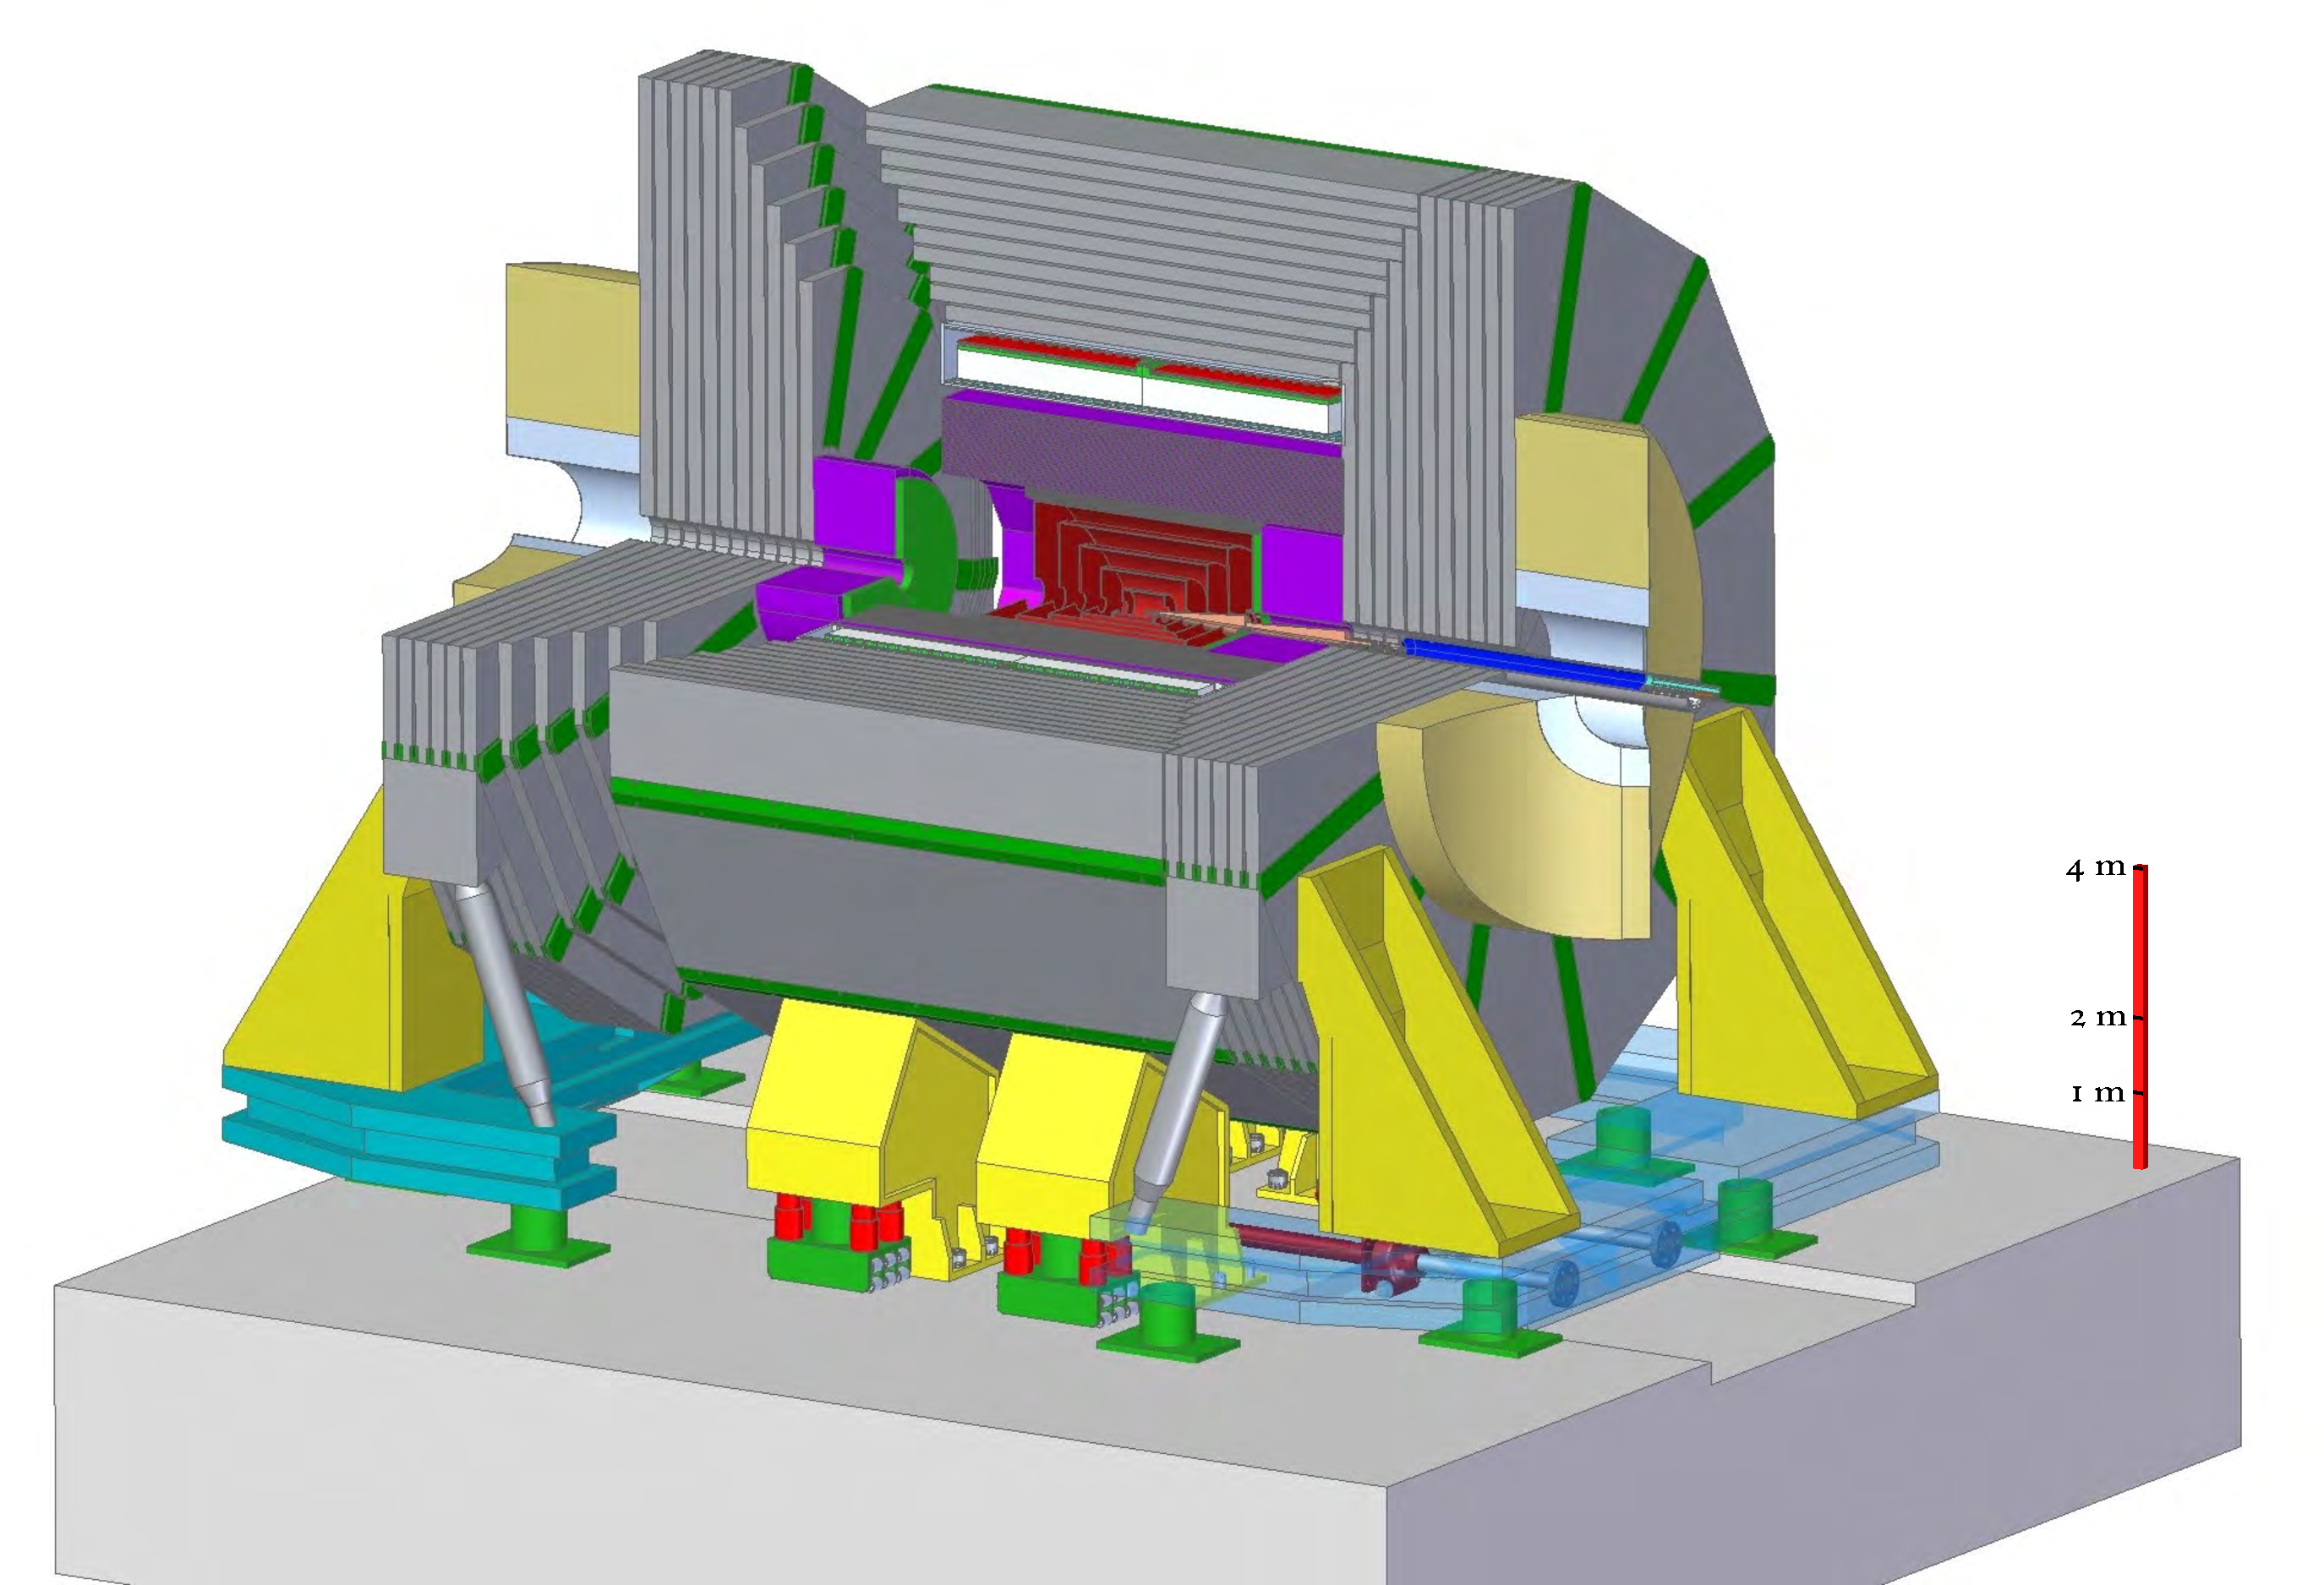
\includegraphics[width=0.9\hsize]{chapters/figures/SiD.pdf}
\caption{The SiD detector concept.
\label{fig_sid}}
 \end{center}
 \vspace{-0.7cm}
 \end{figure}

\thisfloatsetup{floatwidth=\SfigwFull,capposition=beside}
\begin{table}[htbp]
\renewcommand{\arraystretch}{1.25}

\ttabbox{

\caption{\label{sid:ConceptOverview:Table:Ovw_sidparams}Key parameters of the baseline \sid design. (All dimension
are given in cm).}
}
{
\begin{tabular}{l l r r r}
    \toprule
    \sid Barrel& Technology& Inner radius& Outer radius& z extent \\
    \midrule
    Vertex detector& Silicon pixels& 1.4& 6.0& $\pm \quad 6.25$ \\
    Tracker& Silicon strips& 21.7& 122.1& $\pm \quad 152.2$ \\
    ECAL& Silicon pixels-W& 126.5& 140.9& $\pm \quad 176.5$ \\
    HCAL& RPC-steel& 141.7& 249.3& $\pm \quad 301.8$ \\
    Solenoid& 5 Tesla SC & 259.1& 339.2& $\pm \quad 298.3$ \\
    Flux return& Scintillator-steel& 340.2 & 604.2& $\pm \quad 303.3$ \\
    \bottomrule

   \toprule
 \sid Endcap& Technology& Inner z& Outer z& Outer radius \\
    \midrule
Vertex detector& Silicon pixels& 7.3& 83.4& 16.6 \\
Tracker& Silicon strips& 77.0& 164.3& 125.5 \\
ECAL& Silicon pixel-W& 165.7& 180.0& 125.0 \\
HCAL& RPC-steel& 180.5& 302.8& 140.2 \\
Flux return& Scintillator/steel& 303.3& 567.3& 604.2 \\
LumiCal& Silicon-W& 155.7& 170.0& 20.0 \\
BeamCal& Semiconductor-W& 277.5& 300.7& 13.5 \\
    \bottomrule
\end{tabular}
}

\end{table}

\subsubsection{Silicon-based Tracking}
The tracking system (Fig.~\ref{fig:fig_vxdtrk}) is a key element of the ILC detector concepts. The
particle flow algorithm requires excellent tracking with superb efficiency and
two-particle separation. The requirements for precision measurements, in
particular in the Higgs sector, place high demands on the momentum resolution at
the level of $\delta (1/\pT)  \sim 2-5 \times 10^{-5}/$GeV/$c$.

Highly efficient charged particle tracking is achieved using the pixel detector
and main tracker to recognise and measure prompt tracks, in conjunction with the ECAL, which can
identify short track stubs in its first few layers 
to catch tracks arising from secondary decays of long-lived particles. With
the choice of a 5~T solenoidal magnetic field, in part chosen to control the \epem pair
background, the design allows for a compact tracker design. 

\begin{figure}[tb]
 %\epsfysize=9.0cm
 \begin{center}
 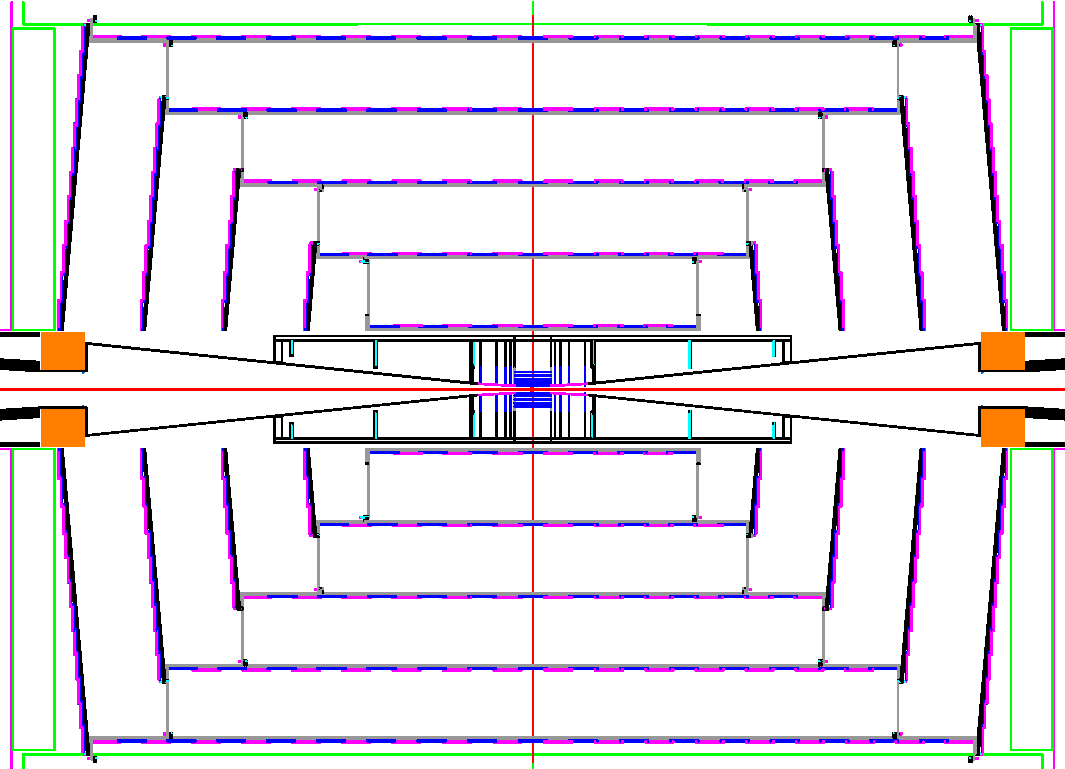
\includegraphics[width=0.9\hsize]{chapters/figures/vxdtrk.pdf}
\caption{r-z view of vertex detector and outer tracker.
\label{fig_vxdtrk}}
 \end{center}
 \vspace{-0.7cm}
 \end{figure}

\subsubsection{Vertex detector}

To unravel the underlying physics mechanisms of new observed processes, the
identification of heavy flavours will play a critical role. One of the main
tools for heavy flavour identification is the vertex detector. The physics goals
dictate an unprecedented spatial three-dimensional point resolution and a very
low material budget to minimise multiple Coulomb scattering. The running 
conditions at the ILC impose the readout speed and radiation tolerance. 
These requirements are normally in tension. High
granularity and fast readout compete with each other and tend to increase the
power dissipation. Increased power dissipation in turn leads to an increased
material budget. The challenges on the vertex detector are considerable and
significant R\&D is being carried out on both the development of the sensors and
the mechanical support.
The \sid vertex detector uses a barrel and disk layout. The barrel section
consists of five silicon pixel layers with a pixel size of
$20~\times~20~\micron^2$. The forward and backward regions each have four
silicon pixel disks. In addition, there are three silicon pixel disks at a
larger distance from the interaction point to provide uniform coverage for the
transition region between the vertex detector and the outer tracker. This
configuration provides for very good hermeticity with uniform coverage and
guarantees excellent charged-track pattern recognition capability and impact parameter resolution 
over the full solid angle. 
This enhances the capability of the integrated tracking system and, 
in conjunction with the high magnetic field, makes for a very compact
system, thereby minimising the size and costs of the calorimetry.

To provide for a very robust track-finding performance the baseline 
choice for the vertex detector has a sensor technology that provides
time-stamping of each hit with sufficient precision to assign it to
a particular bunch crossing. This significantly suppresses
backgrounds. 

Several technologies are being developed. One of them is a CMOS-based
monolithic pixel sensor called Chronopixel. The main goal for the design is a
pixel size of about $10~\times~10~\micron^2$ with 99\% charged-particle
 efficiency. Prototype devices have demonstrated that the concept works; 
what should be a fully functional chip is presently under test. More 
challenging is the 3D vertical integrated silicon technology, for which a full 
demonstration is also close.

Minimising the support material is critical to the development of a high-performance 
vertex detector. An array of 
low-mass materials such as reticulated foams and silicon-carbide
materials are under consideration. An alternative approach that is being pursued very actively is the
embedding of thinned, active sensors in ultra low-mass media. This line of R\&D
explores thinning active silicon devices to such a thickness that the silicon
becomes flexible. The devices can then be embedded in, for example, Kapton
structures, providing extreme versatility in designing and constructing a vertex
detector.

Power delivery must be accomplished without exceeding the material budget and
over heating the detector.  The vertex detector 
design relies on power pulsing during bunch trains to minimise heating 
and uses forced air for cooling. 

\subsubsection{Main tracker}
The main tracker technology of
choice is silicon strip sensors arrayed in five nested cylinders in the central
region and four disks following a conical surface with an angle of 5 degrees
with respect to the normal to the beamline in each of the end regions. The geometry of the endcaps
minimises the material budget to enhance forward tracking. The detectors are
single-sided silicon sensors, approximately 10 $\times$ 10 cm$^2$ with a readout
pitch of 50~\micron. The endcaps utilise two sensors bonded back-to-back for
small angle stereo measurements. With an outer cylinder radius of 1.25~m
and a 5~T field, the charged track momentum resolution will be better than
$\delta (1/\pT) = 5 \times 10^{-5} $/(GeV/$c$) for high momentum tracks with coverage down to polar angles of 10 degrees.

The all-silicon tracking approach has been extensively tested using full Monte-Carlo
simulations including full beam backgrounds. Besides having an excellent momentum resolution
it provides robust pattern recognition even in the presence of backgrounds and has a
real safety margin, if the machine backgrounds will be worse than expected.

\subsubsection{Main calorimeters}

The \sid baseline design incorporates the elements needed to
successfully implement the PFA approach. This imposes a number of
basic requirements on the calorimetry. The central calorimeter
system must be contained within the solenoid in order to reliably associate
tracks to energy deposits. The electromagnetic and hadronic sections
must have imaging capabilities that allow both efficient
track-following and correct assignment of energy clusters to tracks. These
requirements imply that the calorimeters must be finely segmented both
longitudinally and transversely. In order to ensure that no significant amount
of energy can escape detection, the calorimetry must extend down to small
angles with respect to the beampipe and must be sufficiently deep to prevent
significant energy leakage. Since the average penetration depth of a hadronic
shower grows with its energy, the calorimeter system must be designed for the
highest-energy collisions envisaged.

In order to ease detector construction the calorimeter mechanical design consists of a series of modules of
manageable size and weight. The boundaries between
modules are kept as small as possible to prevent significant non-instrumented
regions. The detectors are designed to have excellent long-term stability and reliability,
since access during the data-taking period will be extremely limited, if not
impossible.

The combined ECAL and HCAL systems consist of a
central barrel part and two endcaps, nested inside the barrel. The entire barrel system is contained
within the volume of the cylindrical superconducting solenoid. 

The
electromagnetic calorimeter has silicon active layers between tungsten absorber
layers. The active layers use 5$\times$5~mm$^2$ silicon pixels, which provide excellent spatial resolution.
The structure has 30 layers in total, the first 20 layers having a
thinner absorber than the last ten layers. This configuration is a 
compromise between cost, electromagnetic shower radius, sampling frequency, and
shower containment. The total depth of the electromagnetic calorimeter is 26
radiation lengths (\xo) and one nuclear interaction length. 

The hadronic
calorimeter has a depth of 4.5 nuclear interaction lengths, consisting of
alternating steel plates and active layers. The baseline choice for the active
layers is scintillator tiles read out via silicon photomultipliers. For this approach SiD is closely following the analog hadron calorimeter developments within the CALICE collaboration.

\subsubsection{Forward calorimeters}

Two special calorimeters are foreseen in the very forward region: LumiCal for precise measurement, and BeamCal for fast
estimation, of the luminosity. LumiCal and BeamCal are
compact cylindrical electromagnetic calorimeters centred on the outgoing beam.
They are based on 30 layers' depth of semiconductor-tungsten technology. BeamCal
is placed just in front of the final focus quadrupole and LumiCal is aligned
with the electromagnetic calorimeter endcap. LumiCal uses silicon sensor readout.
It is a precision device with
challenging requirements on the mechanics and position control. BeamCal is
exposed to a large flux of low-energy electron-positron pairs originating from
beamstrahlung. These depositions, useful for a bunch-by-bunch luminosity
estimate and the determination of beam parameters, require radiation hard
sensors. The detectors in the very forward region have to tackle relatively high
occupancies, requiring dedicated front-end electronics.

The challenge for BeamCal is to find sensors that will tolerate about one MGy
of dose per year. So far polycrystalline chemical vapour deposition (CVD) diamond
sensors of area 1~cm$^2$ and larger sectors of GaAs pad sensors have been studied. Since
large-area CVD diamond sensors are extremely expensive, they may be used for only
the innermost part of BeamCal. At larger radii GaAs sensors appear to be a
promising option. Sensor samples produced using the liquid encapsulated
Czochralski method have been studied in a high-intensity electron beam. 

For SiD,
the main activities are the study of these radiation-hard sensors, development
of the first version of the so-called Bean readout chip, and the simulation of BeamCal
tagging for physics studies. SiD coordinates these activities with the FCAL R\&D Collaboration. 

\subsubsection{Magnet Coil}

The \sid superconducting solenoid is based on the CMS solenoid
design philosophy and construction techniques, using a slightly modified CMS
conductor as its baseline design. Superconducting strand count in the coextruded
Rutherford cable was increased from 32 to 40 to accommodate the higher 5~T
central field. 

Many iron flux return configurations have been simulated in two
dimensions so as to reduce the fringe field. An Opera 3D calculation with the Detector
Integrated Dipole (DID) coil has been completed.
Calculations of magnetic field with a 3D ANSYS program
are in progress. These will have the capability to calculate forces and stress
on the DID as well as run transient cases to check the viability of using the
DID as a quench propagator for the solenoid. Field and force calculations with
an iron endcap HCAL were studied. The field homogeneity improvement was found
to be insufficient to pursue this option. 

Conceptual DID construction and
assembly methods have been studied. The solenoid electrical power system,
including a water-cooled dump resistor and grounding, was established.
Significant work has been expended on examining different conductor stabiliser
options and conductor fabrication methods. This work is pursued as a cost- and
time-saving effort for solenoid construction.

\subsubsection{Muon System}
The flux-return yoke is instrumented with position sensitive detectors to
serve as both a muon filter and a tail catcher. The total area to be
instrumented is very significant - several thousand square meters. Technologies
that lend themselves to low-cost large-area detectors are therefore under
investigation. Particles arriving at the muon system have seen large amounts of
material in the calorimeters and encounter significant multiple scattering
inside the iron. Spatial resolution of a few centimetres is therefore
sufficient. Occupancies are low, so strip detectors are possible. The \sid
baseline design uses scintillator technology, with RPCs as an alternative. 
The scintillator technology uses extruded scintillator readout with wavelength 
shifting fibre and SiPMs, and has been successfully demonstrated. 
Simulation studies have shown that nine or more layers of sensitive detectors 
yield adequate energy measurements and good muon-detection efficiency and purity.


\subsubsection{The Machine-Detector Interface}
A time-efficient implementation of the push-pull model of
operation sets specific requirements and challenges for many detector and
machine systems, in particular the interaction region (IR) magnets, the
cryogenics, the alignment system, the beamline shielding, the detector design
and the overall integration. The minimal functional requirements and interface
specifications for the push-pull IR have been successfully developed and
published~\cite{Platform_Agreement,IR_Layout}, to which all further IR design
work on both the detectors and machine sides are constrained.

\subsection{The ILD Detector}
The ILD detector is a proposed detector for the international linear collider, ILC. It has been developed by a proto-collaboration with the goal to develop and eventually propose a fully integrated detector for the ILC. 

The ILD detector concept has been designed as a multi-purpose detector. It should deliver excellent physics performance for collision energies between 90~Gev and 1~TeV, the largest possible energy reach of the ILC. The ILD detector has been optimized to perform excellently at the initial ILC energy of 250 GeV (for more details see \cite{ild:bib:ILDloi}, \cite{ild:bib:ILDDBD}).

The science which will be done at the ILC requires a true multi-purpose detector. A central element of the design has been the capability of the detector to reconstruct precisely complex hadronic final states as well as more events with leptons or missing energy in the final state. Thus traditional precision detector elements as vertex detectors are combined in an overall design philosophy called particle flow, which has been developed for optimal hadronic event reconstruction.

The high precision vertex detector positioned very closely to the interaction point is followed by a hybrid tracking layout, realised as a combination of silicon tracking with a time projection chamber, and a calorimeter system. The complete system is located inside a large solenoid providing a magnetic field of 3.5-4 T. On the outside of the coil, the iron return yoke is instrumented as a muon system and as a tail catcher calorimeter. 

The vertex detector is realised as a multi-layer pixel-vertex detector (VTX), with three super-layers each comprising two layers. The detector has a pure barrel geometry. To minimise the occupancy from background hits,
the first super-layer is only half as long as the outer two. Whilst the underlying detector technology has not yet been decided, 
the VTX is optimised for point resolution and minimum material thickness. 
	
A system of silicon strip and pixel detectors surrounds the VTX detector. In the barrel, two layers of silicon strip detectors (SIT) are arranged to bridge the gap between the VTX and the TPC. In the forward region, a system of two silicon-pixel disks and five silicon-strip disks (FTD) provides low angle tracking coverage.

A distinct feature of ILD is a large volume time projection chamber (TPC) with up to 224 points per track. The TPC is optimised for 3-dimensional point resolution and minimum material in the field cage and in the end-plate. It also allows d$E$/d$x$ based particle identification. At the ILC a TPC has a number of specific strength, which make this type of detector attractive. A time projection chamber offers true three-dimensional points, and offers many of those along a charged particle trajectory. The intrinsic disadvantage of a TPC, its slow readout speed, does not really harm the performance at the ILC, since the time between bunches is relativly long, with around 300~ns. On the other hand the large number of points offer superb pattern recognition capabilities, and allows the detailed reconstruction of kinks or decays in flight within its volume. This can be achieved at a very low material budget, rather uniforly distributed over the sensitive volume. The excellent performance of the system is particularly striking at low momenta, at a few GeV and below, where the combination of three dimensional reconstruction and low material allows the efficient and precise reconstruction of tracks. 

Outside the TPC a system of Si-strip detectors in between the TPC and the ECAL (SET), provide additional high precision space points which improve the tracking performance and provide additional
    redundancy in the regions between the main tracking volume and the calorimeters. 

A highly segmented electromagnetic calorimeter (ECAL) provides up to 30 samples in depth and small transverse cell size, split into a barrel and an end cap system. For the absorber Tungsten has been chosen, for the sensitive area silicon diodes or scintillator strips are considered.
\thisfloatsetup{floatwidth=\SfigwFull,capposition=beside}
\begin{figure}[t!]
\begin{tabular}{cc}
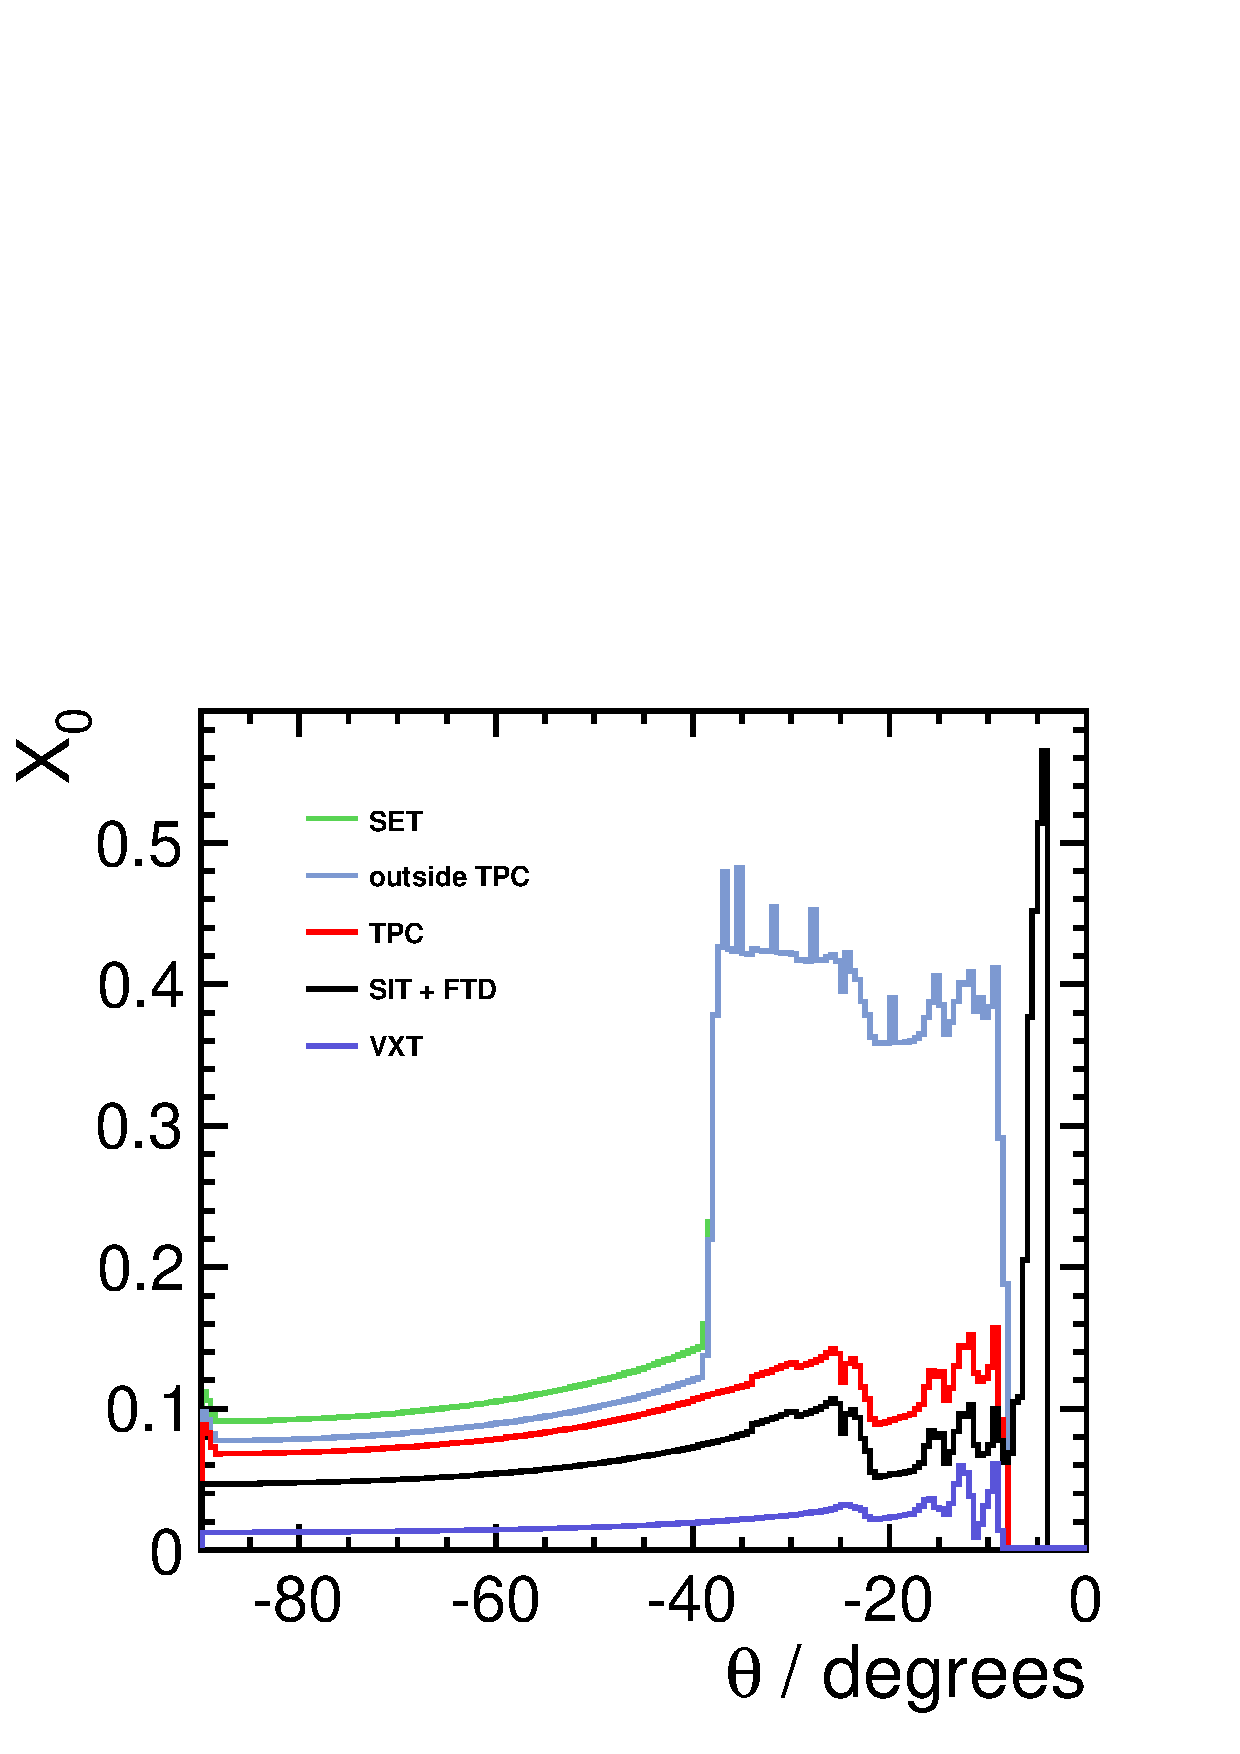
\includegraphics[width=0.52\hsize,viewport={0 -10 600 500},clip]{Introduction/fig/material-budget-new.pdf} &
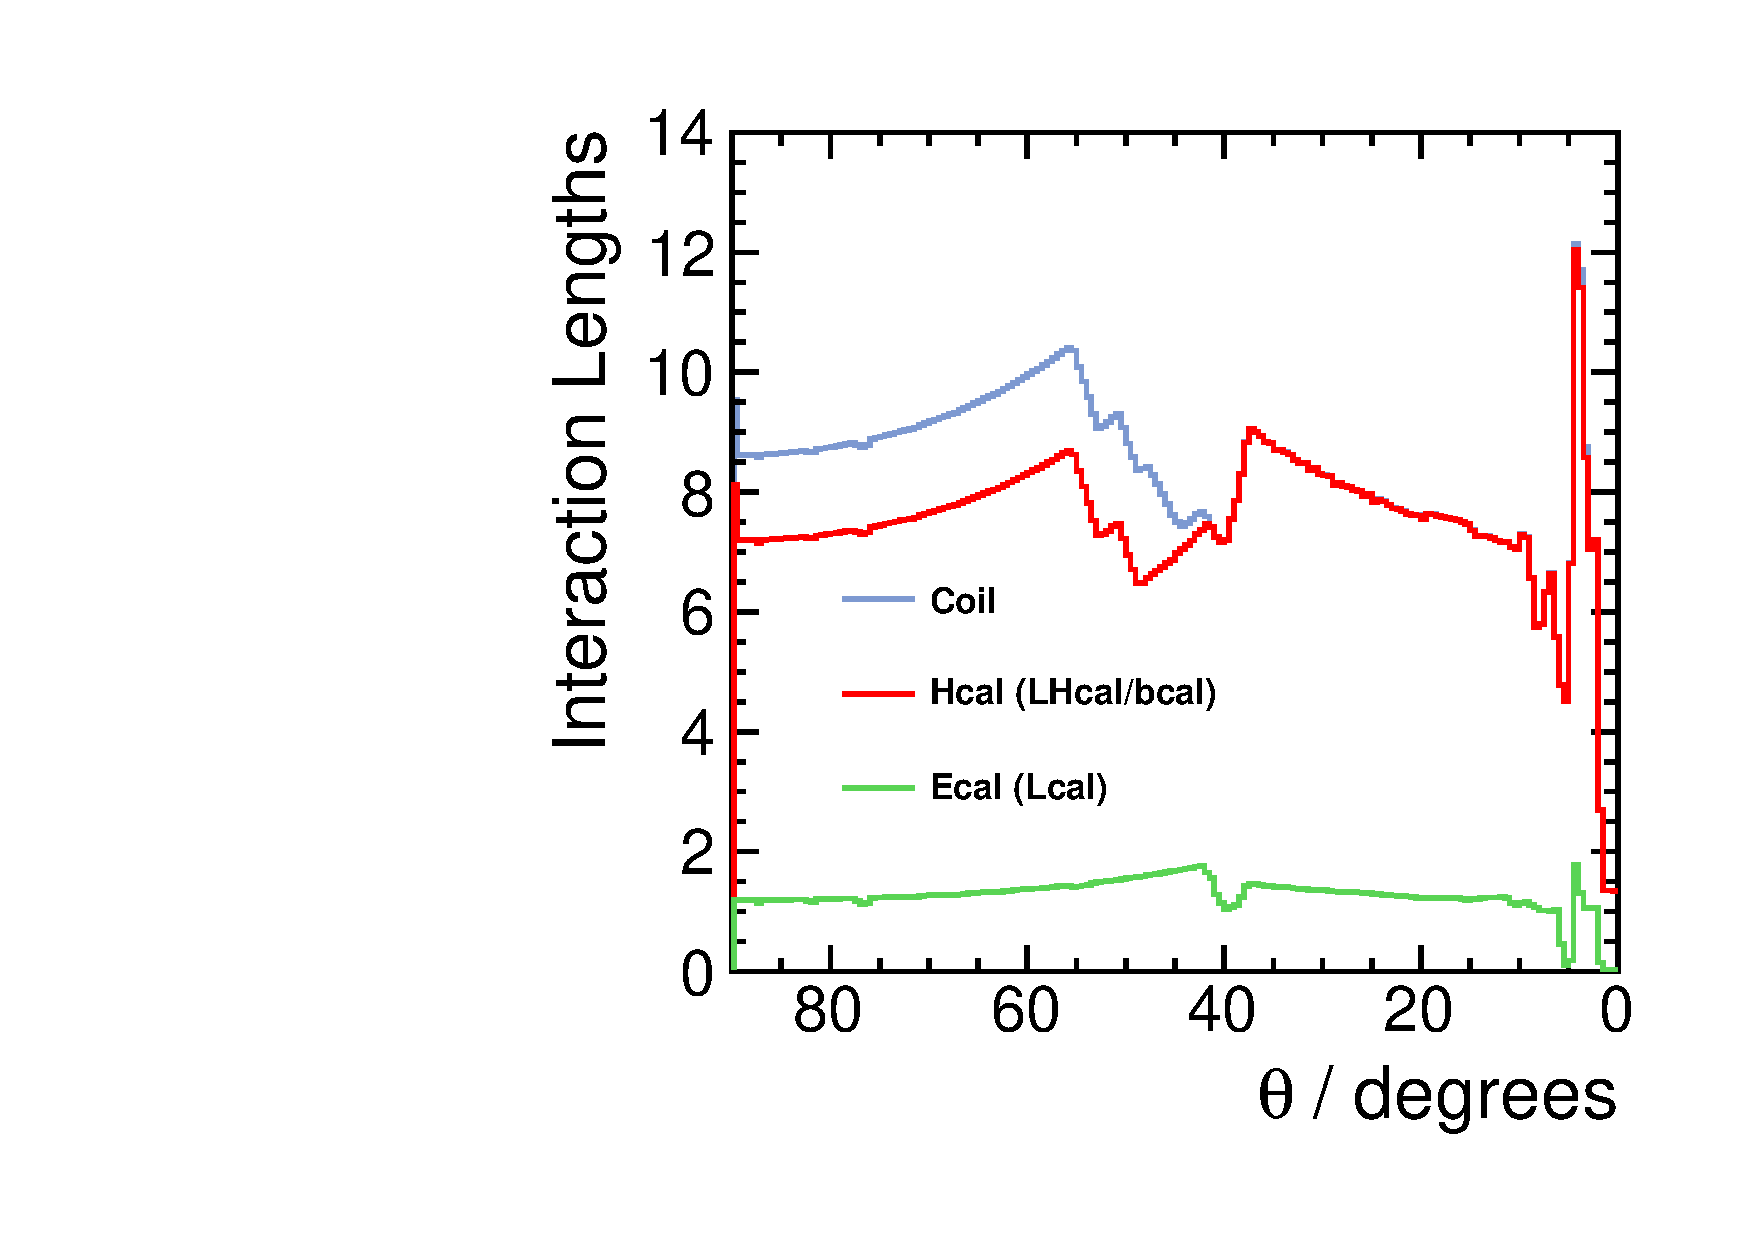
\includegraphics[width=0.5\hsize]{Introduction/fig/intlen_ILD_o1_v05.pdf}
\end{tabular}
\caption[Material in the ILD detector]{Left: Average total radiation length of the material
  in the tracking detectors as a function of polar angle. Right: Total interaction length in the detector, up to the end of the calorimeter system, and including the coil of the detector.}
%\end{figure}
\label{fig:intro:material}
%\begin{tabular}{cc}

\end{figure}

This is followed by a segmented hadronic calorimeter (HCAL) with up to 48 longitudinal samples and small transverse cell size. Two 
options are considered, both based on a Steel-absorber structure. One option uses scintillator tiles of $3 \times 3$\,cm$^2$, 
which are read out with an analogue system. The second uses a gas-based readout which allows a $1 \times 1$\,cm$^2$ 
cell geometry with a semi-digital readout of each cell. 

At very forward angles, below the coverage provided by the ECAL and the HCAL, a system of high precision and radiation hard calorimetric detectors (LumiCAL, BeamCAL, LHCAL) is foreseen. These
extend the calorimetric coverage to almost $4\pi$, measure the luminosity, and  monitor the quality of the colliding beams.

A large volume superconducting coil surrounds the calorimeters, creating an axial $B$-field of nominally 3.5-4\,Tesla.

An iron  yoke, instrumented with scintillator strips or resistive plate chambers (RPCs), returns the magnetic flux of the solenoid, and, at the same time, serves as a muon filter, muon detector and tail catcher calorimeter.

\thisfloatsetup{floatwidth=\SfigwFull,capposition=beside}
\begin{figure}[b!]
\begin{tabular}{cc}

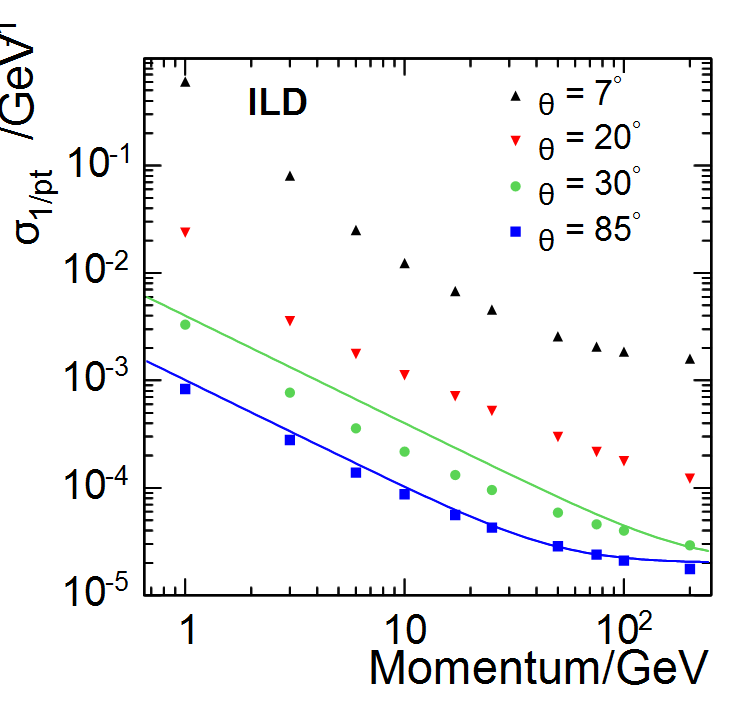
\includegraphics[width=0.5\hsize]{Introduction/fig/deltaInvP_all_fits.png} &
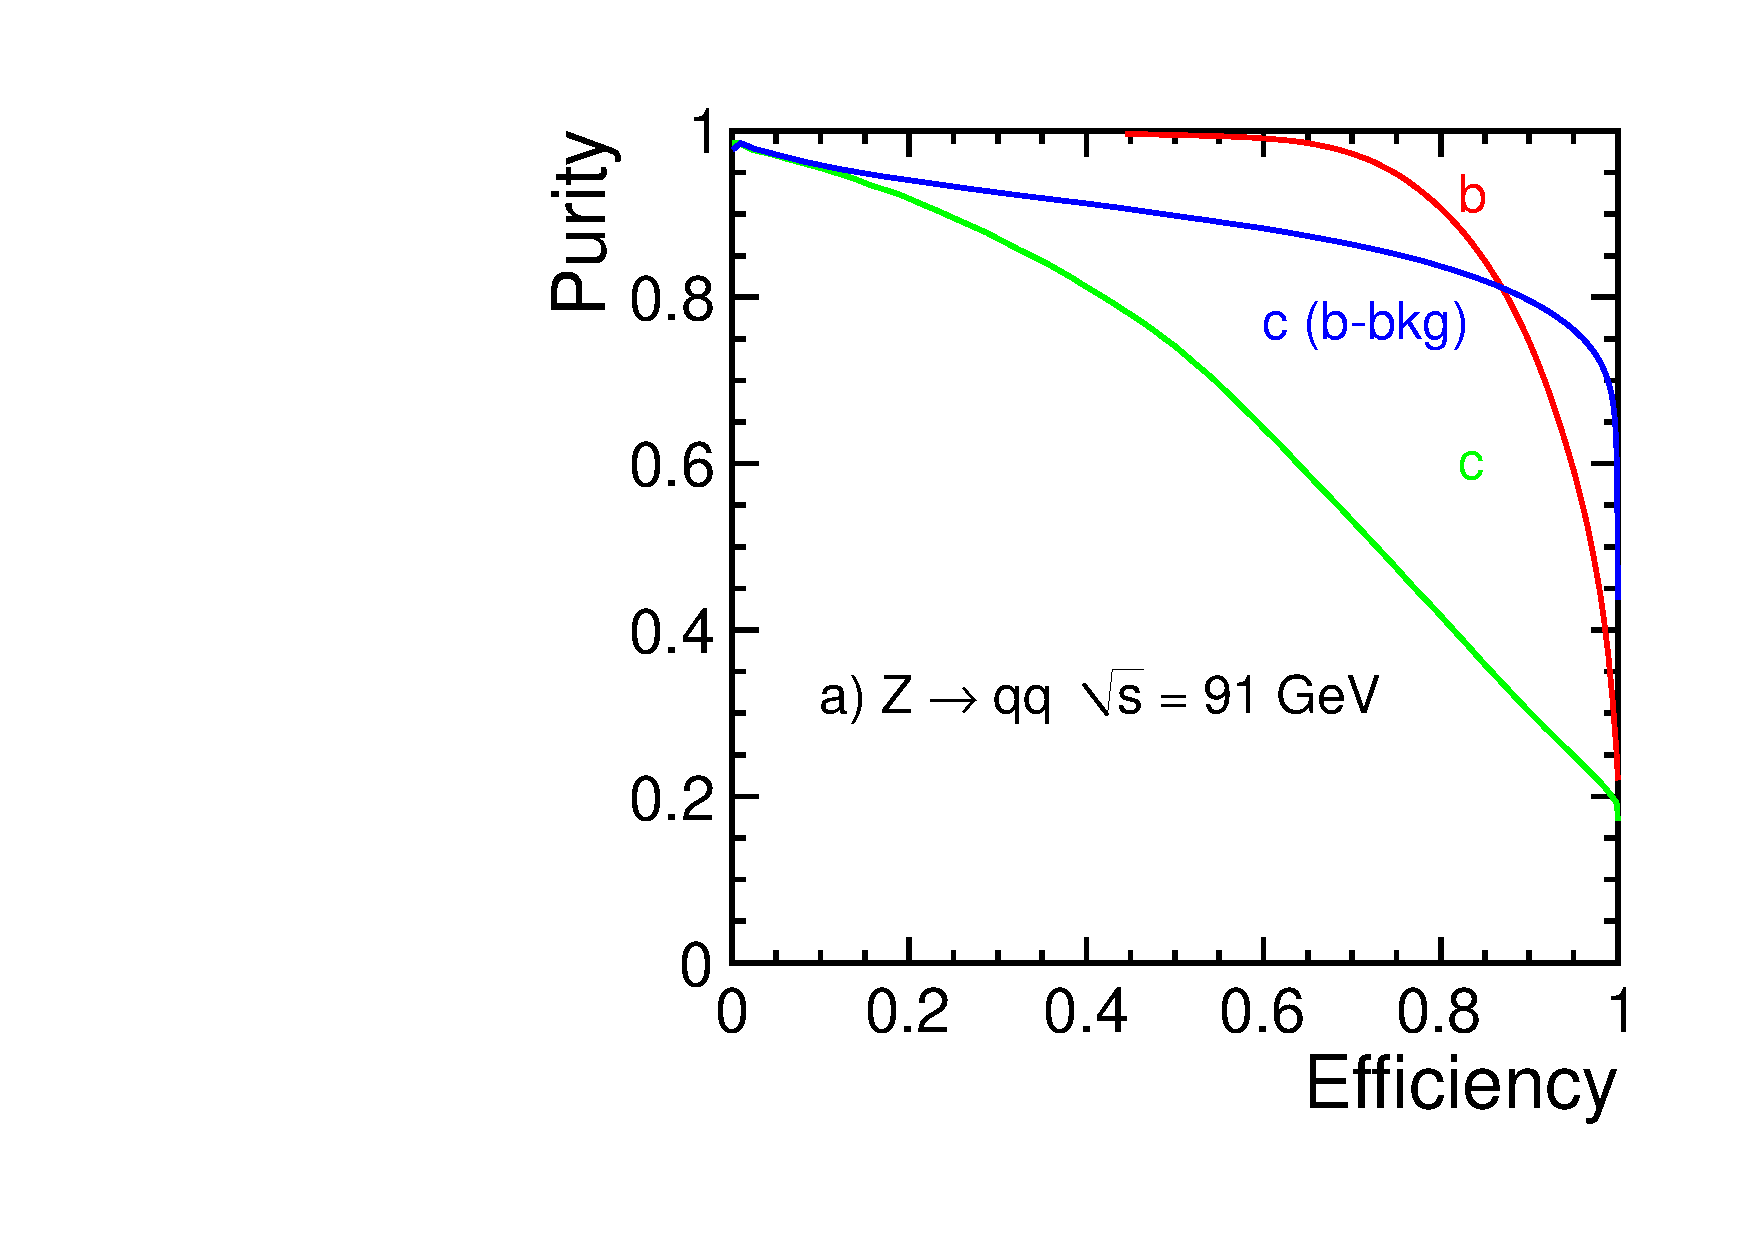
\includegraphics[width=0.5\hsize]{Introduction/fig/evalZ-lcfiweights_qq91new_v02-test.pdf}
\end{tabular}
\caption{\label{ild:fig:intro:tracking}(left) Momentum resolution for the ILD detector concept, as a function of the transverse momentum of the particle. (right) Flavour tagging efficiency versus purity for bottom events in sample of Z decays at 91\,GeV, and for charm events with only bottom background. )}
\end{figure}



\begin{figure}[t!]

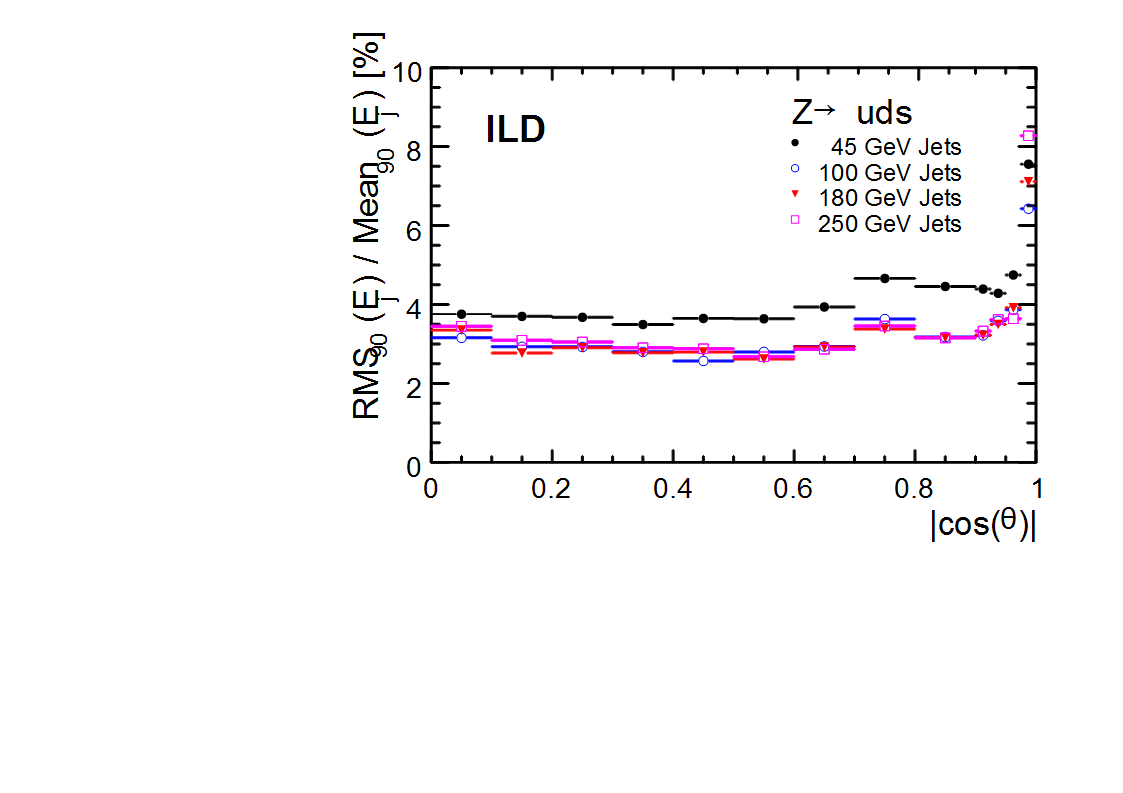
\includegraphics[width=0.8\hsize]{Introduction/fig/ild01_o1_pflow.png}

\caption{\label{ild:fig:intro:pflow}Fractional jet energy resolution
    plotted against $|\cos\theta|$ where theta is the polar angle of the thrust axis of the event. }
\end{figure}

%The main parameters of the ILD detector are summarised in Table~\ref{ild:tab:barrelpara} and table~\ref{ild:tab:endcappara}.
%\begin{sidewaystable}[thb]


The performance of the ILD concept has been extensively studied using a detailed GEANT4 based simulation model and sophisticated reconstruction tools. Backgrounds have been taken into account to the best of current knowledge. 

the key technologies proposed for the ILD detector have been developed in close cooperation with R\&D collaborations and have been extensively tested. The performance numbers of key systems are based on results from prototypes, whereever possible, and extraploated to the full detector performance. This strong check against experimental results ensures that the performance numbers are reliable and are considered a realistic estimate of the ultimate detector performance. 


A key characteristics of the detector is the amount of material in the detector. Particle flow requires a thin tracker, to minimise interactions before the calorimeters, and thick calorimeters, to fully absorb the showers. Figure~\ref{ild:fig:intro:material}~(left) shows the material in the detector in radiation lengths, until the entry of the calorimeter. The right plot shows the total interaction length including the calorimeter system. 

The performance of the tracking system can be summarised by its combined momentum resolution, shown in Figure~\ref{ild:fig:intro:tracking}~(left). A resolution of $\sigma_{1/p_T} = 2 \times 10^{-5}$\,GeV$^{-1}$ has been achieved for high momenta. For many physics studies the tagging of long lived particles is of key importance. Several layers of pixel detectors close to the IP allow the reconstruction of displaced vertices, as shown in Figure~\ref{ild:fig:intro:tracking}~(right).




Calorimeter system and tracking system together enter into the particle flow performance. The performance of the ILD detector for different energies and as a function of the polar angle is shown in Figure~\ref{ild:fig:intro:pflow}. 

The few plots shown in this section illustrate the anticipated performance of the detector and illustrate the potential for precision measurements with the ILD detector. 


\section{\label{sec:software}Software and Monte-Carlo samples: Modeling the experimental environment}

   10 pages Gaede + Miyamoto
   
   %
% some useful macros
%
\newcommand{\fix}[1]{\textcolor{red}{\texttt{#1}}} % command for comments 
%\newcommand{\fix}[1]{} % remove all comments

\newcommand{\CPP}{C\nolinebreak\hspace{-.05em}\raisebox{.4ex}{\tiny\bf +}\nolinebreak\hspace{-.10em}\raisebox{.4ex}{\tiny\bf +}}


%Description of ILC software and computing requirements] }

\fix{ PLEASE DO NOT EDIT THIS PART IN OVERLEAF! This is work in progress!}

%Description of ILC software and computing requirements] }


\subsection{Software}

More than 15 years ago the linear collider community has started to develop common software
tools to facilitate the development and optimization of detector concepts based on realistic
simulations of physics interactions. These software tools eventually led to the creation of
a common software ecosystem called \emph{iLCSoft}~\cite{bib:ilcsoft}.
The \emph{iLCSoft} tools are used by both ILC detector concepts as well as by CLIC
and partly by CEPC and FCC.

From the start, a strong emphasis has been placed on developing flexible and generic tools
that can easily be applied to other experiments or new detector concepts. 
This approach of developing common tools wherever possible has helped considerably in
leveraging the limited manpower and putting the focus on algorithm development that
is crucial for the physics performance. 

In the next sections we will introduce the most relevant tools and algorithms and
describe their design and performance, thereby following the natural flow of data processing
from generated 4-vectors to high level physics objects.


\subsubsection{Core Software Tools}

The foundation for the development of common software was laid with LCIO~\cite{Gaede:2003ip}, the
event data model (EDM) and persistency tool for linear collider studies. At the core of LCIO is a hierarchical
EDM for any particle physics experiment, as shown in Fig.\ref{fig:lcio_edm}.
%%%%%%%%%%%%%%%%
\begin{figure}
\begin{center}
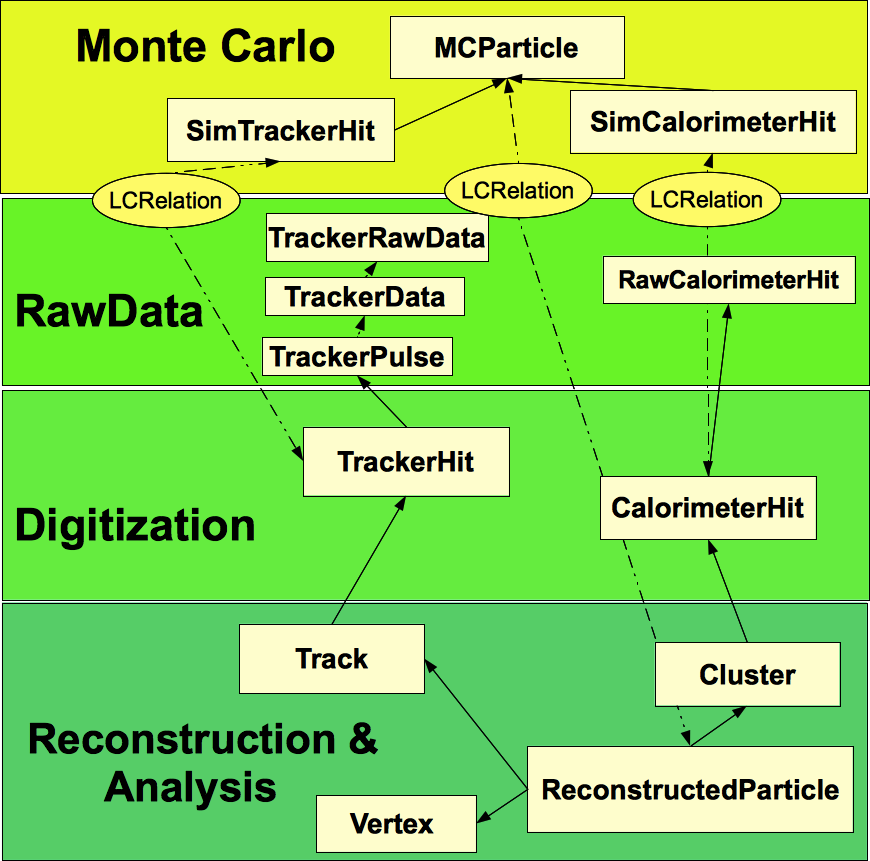
\includegraphics[width=0.60\hsize]{chapters/figures/lcio_edm_schema.png}
\end{center}
\caption{Schematic view of the hierarchical EDM in LCIO.}
\label{fig:lcio_edm}
\end{figure}
%%%%%%%%%%%%%%%%%
It provides data classes for all phases of the event processing, starting from Monte Carlo truth information,
over raw data and digitization to the final reconstruction and analysis. Objects at higher levels of the processing
point back to the lower level constituting objects. As a specific design decision, there are no pointers back to the
Monte Carlo truth but these can be added if needed using dedicated generic LCRelation objects.
These relation objects can be used to create many-to-many relations between arbitrary types in the EDM.
A special class LCGenericObject holds user defined data in named vectors of types int, float and double.
This feature is used in many test beams for conditions data and raw data from the DAQ.
LCIO provides APIs in \CPP, Java and Fortran, where today \CPP\ is used almost exclusively.


The \CPP\ application framework Marlin~\cite{Gaede:2006pj} provides an easy to use environment for developing software
modules on all levels of processing and uses LCIO as its transient data format, i.e. all data that is read in or created
by a software module (called \emph{Processor}) are stored in the \emph{LCEvent} class from LCIO. Marlin processors
are self-documenting and controlled via xml-steering files. As processors have well defined input and output data, Marlin
provides a \emph{"Plug-And-Play"} environment, where any specific algorithm can easily be exchanged with another
equivalent implementation for direct comparisons and benchmarking.


The generic detector description toolkit DD4hep~\cite{Frank:2014zya,Frank:2015ivo} provides a powerful tool for describing
the detector geometries, materials and readout properties. DD4hep follows a modular component based approach and provides
interfaces to full simulations with Geant4~\cite{Agostinelli:2002hh} via DDG4, to reconstruction programs via DDRec and to
conditions data and alignment with DDCond and DDAlign respectively, see Fig.\ref{fig:dd4hep}.
%%%%%%%%%%%%%%%%
\begin{figure}
\begin{center}
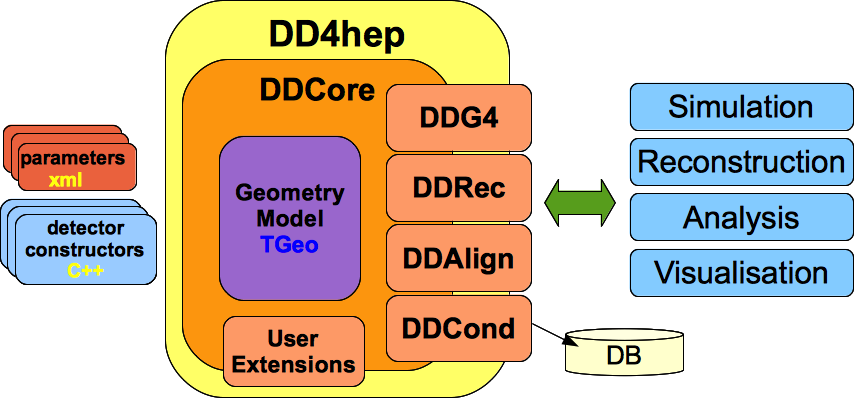
\includegraphics[width=0.90\hsize]{chapters/figures/dd4hep_simple_schema.png}
\end{center}
\caption{Schematic view of DD4hep with its main components and interfaces.}
\label{fig:dd4hep}
\end{figure}
%%%%%%%%%%%%%%%%%
DD4hep is an excellent example for the development of generic software tools for the wider HEP community and was one of the
first incubator projects adopted by the Hep Software Foundation. While it was developed to address the needs of the linear
collider community, it is now used by several other projects and is under evaluation by LHC experiments.



\subsubsection{Event Generators}

Both detector concepts have created large, realistic Monte Carlo samples with the full Standard Model physics as well as various
BSM scenarios that have been used for the physics analyses presented in the following sections.
In a first step, large generator samples with $e^+e^-$-events are created with the Whizard~\cite{Kilian:2007gr} event generator.
Whizard uses tree-level matrix elements and loop corrections to generate events with the final state partons and leptons
based on a realistic beam energy spectrum, the so called \emph{hard sub-process}. The hadronization into the visible final state
is performed with Pythia~\cite{Sjostrand:2006za} tuned to describe the LEP data.

The input spectrum is created with Guinea-Pig~\cite{Schulte:1998au}, a dedicated simulation program for computing
beam-beam interactions at linear colliders. The two dominating effects of the strong beam-beam interactions are the 
beamstrahlung leading to the available luminosity spectrum (see Fig~\ref{fig:lumi_spectrum}) and the creation of
incoherent $e^+e^-$-pairs that are the source of the dominating background at the ILC. These electrons and positrons
are predominantly created in a forward cone as shown in Fig~\ref{fig:pair_bg}. It is this cone that restricts the minimal
allowed radius of the innermost layer of the vertex detector.

%%%%%%%%%%%%%%%%
\begin{figure}
\begin{center}
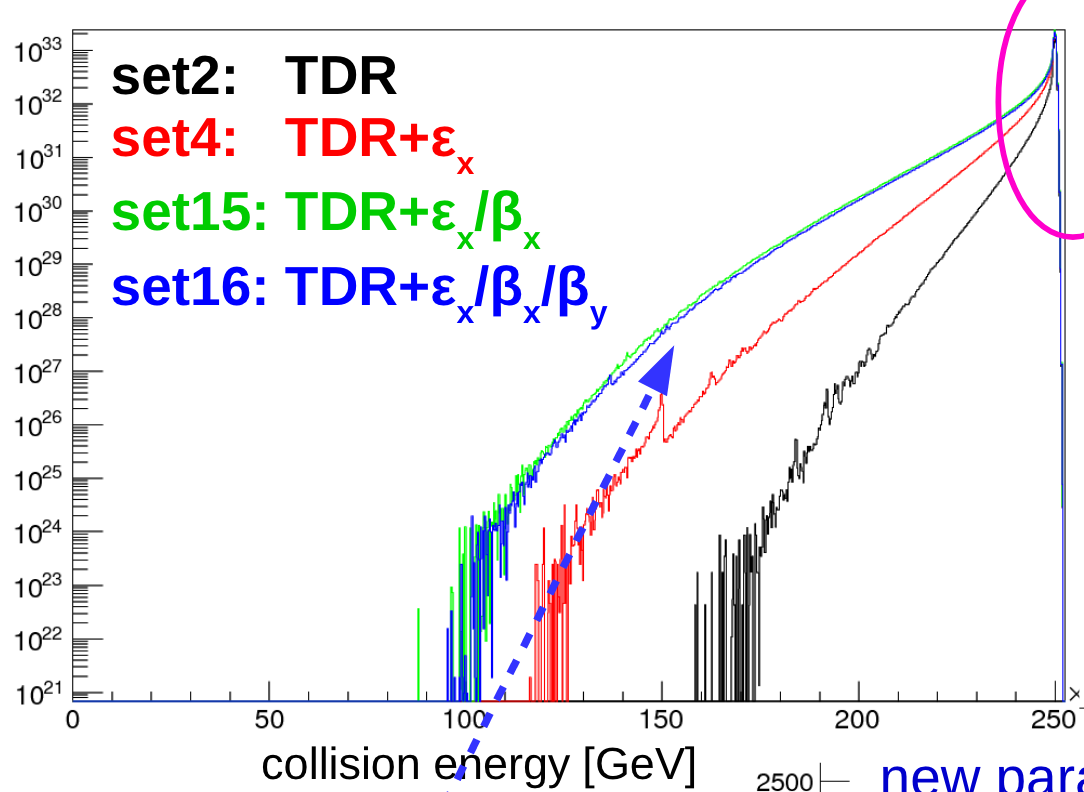
\includegraphics[width=0.80\hsize]{chapters/figures/lumi_spectrum_placeholder.png}
\end{center}
\caption{Luminosity spectrum for 250 GeV.\fix{need nice plot w/ correct spectrum}}
\label{fig:lumi_spectrum}
\end{figure}
%%%%%%%%%%%%%%%%%

%%%%%%%%%%%%%%%%
\begin{figure}
\begin{center}
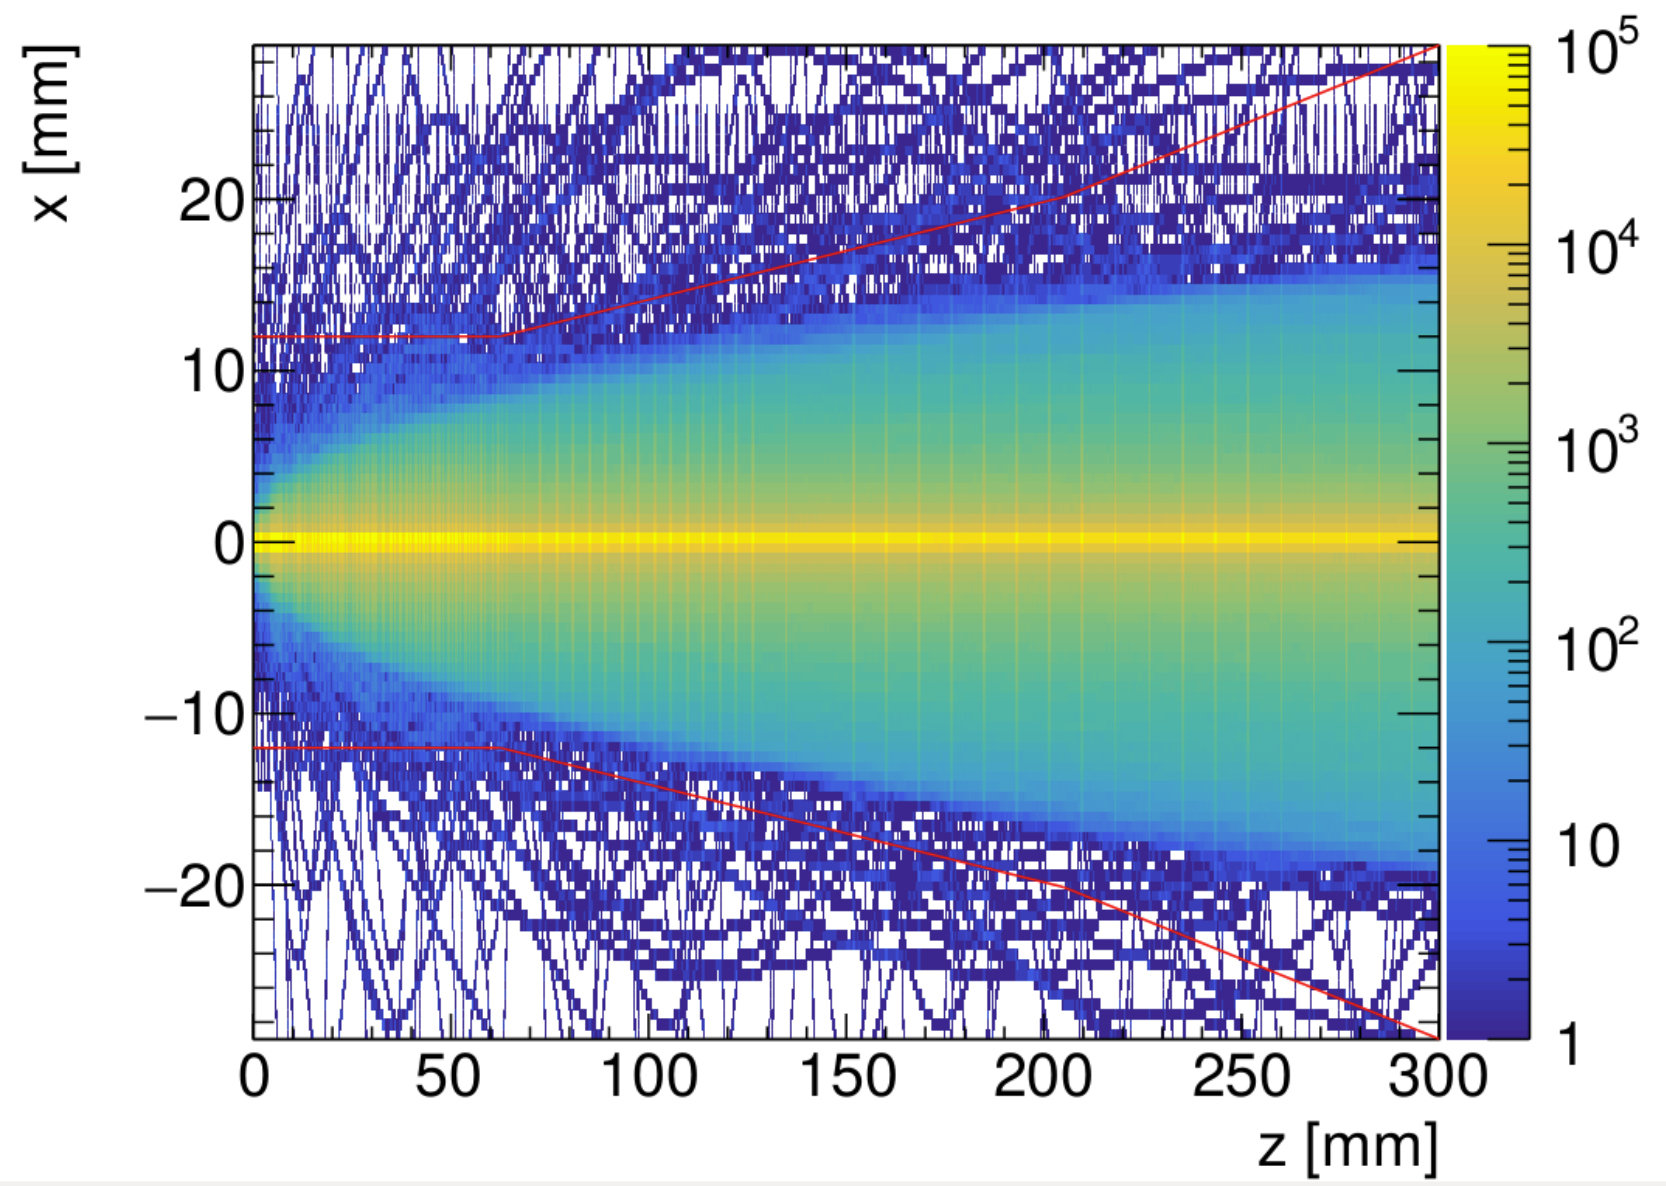
\includegraphics[width=0.90\hsize]{chapters/figures/pair_bg_cone_SiD.png}
\end{center}
\caption{Cone of background from incoherent $e^+e^-$-pairs, generated with Guinea-Pig and simulated in the 5 T B-field of the SiD
  detector (from~\cite{Schutz:2017ihd}).}
\label{fig:pair_bg}
\end{figure}
%%%%%%%%%%%%%%%%%

Another source of background at the ILC are $\gamma \gamma \rightarrow hadrons$ events, due to bremsstrahlung and beamstrahlung photons.
These type of events are generated for $\gamma \gamma$ cms-energies from $300~\rm{MeV~to} ~2~\rm{GeV}.$ with a dedicated generator based
on ~\cite{Chen:1993dba}, for higher energies Pythia is used.


\subsubsection{Simulation}

Both detector concepts have adopted DD4hep for describing their detector simulation models and use \emph{ddsim}, a python application that
is based on the DDG4 component, providing a gateway to full simulations with Geant4.
In DD4hep the detector geometry is implemented in dedicated \CPP modules for every subdetector and the actual parameters with dimensions
and materials are provided via compact xml-files. A large palette of predefined sub-detector drivers exists in DD4hep, allowing for an
easy implementation of a new detector concept by providing suitable compact files.
A dedicated software package lcgeo~\cite{bib:lcgeo}, which is shared by SiD, ILD and CLICdp, contains all subdetector drivers for the
detector concepts under study by these groups, together with the corresponding compact parameter files.

%%%%%%%%%%%%%%%%
\begin{figure}
\begin{center}
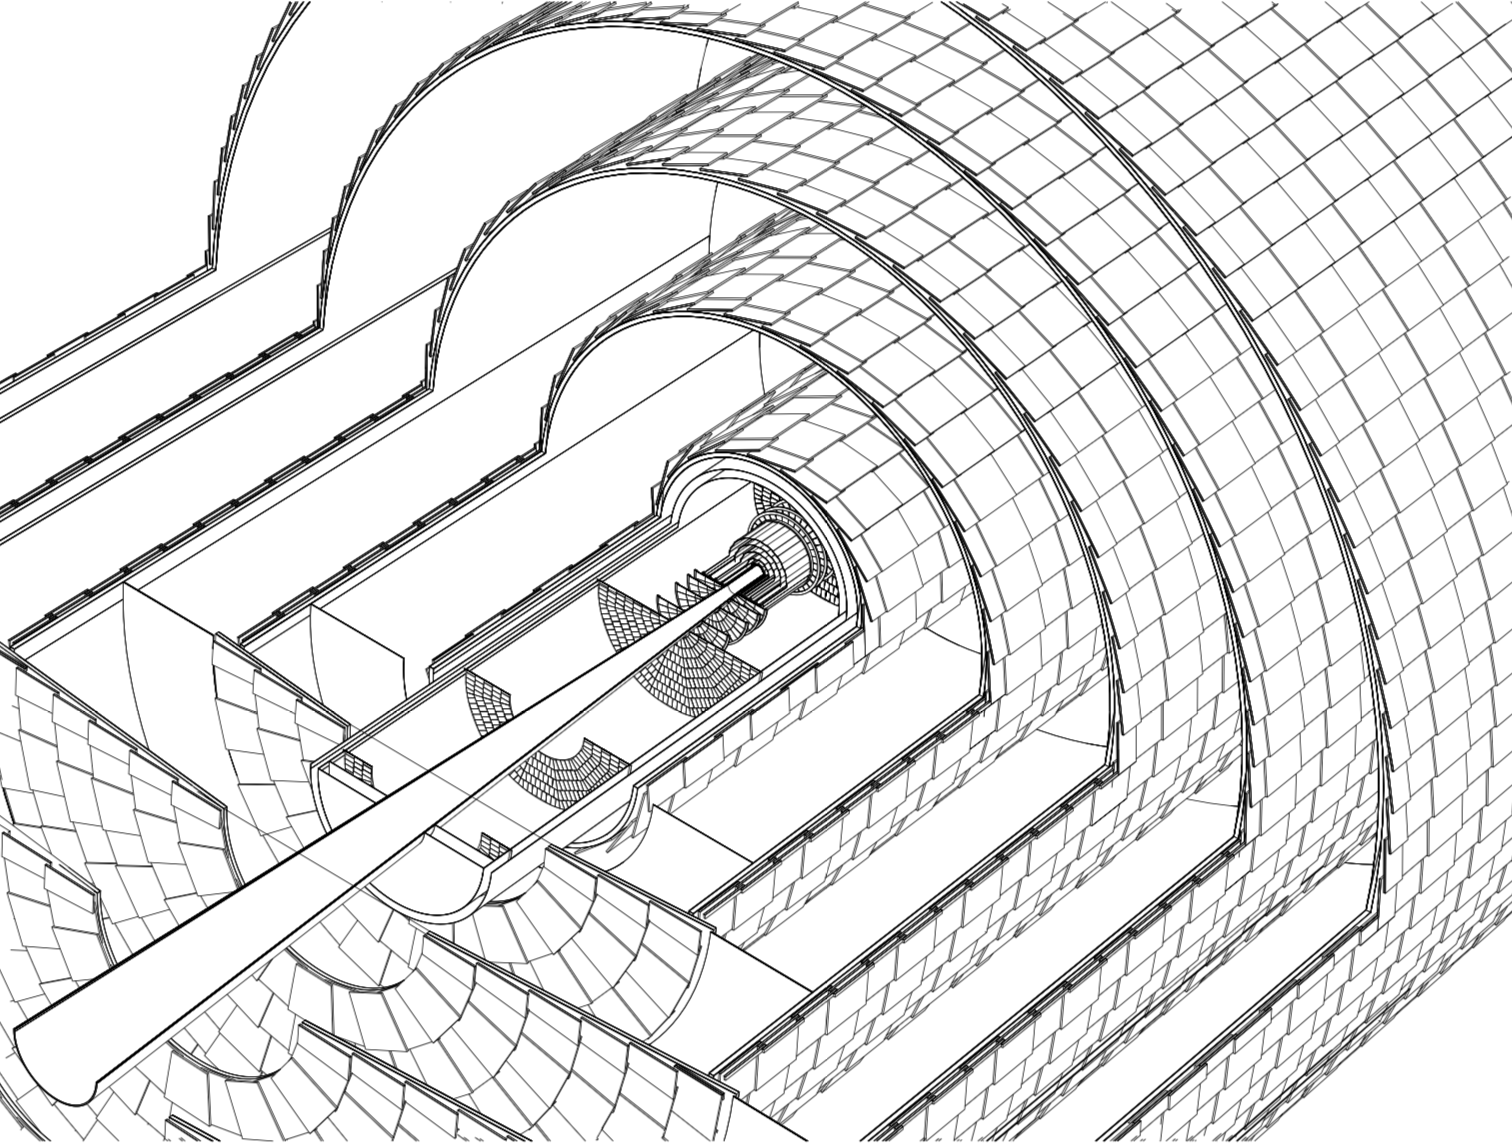
\includegraphics[width=0.80\hsize]{chapters/figures/SiD_tracker_simmodel.png}
\end{center}
\caption{Cut-away view of the tracking system as implemented in the \emph{SIDLOI3} simulation model (from~\cite{Behnke:2013lya}).}
\label{fig:sid_trk}
\end{figure}
%%%%%%%%%%%%%%%%%
Both detector concept groups have invested considerable effort into making their full-simulation models as realistic as possible, by
\begin{itemize}
\item following the exact dimensions and layout of detector elements from engineering models
\item implementing correct material properties
\item implementing precise descriptions of the actual detector technology
\item adding realistic amounts of dead material from supports and services, such as cables and cooling pipes
\item introducing realistic gaps and imperfections into the subdetectors
\end{itemize}
Care has been taken to include realistic material estimates in particular in the tracking region where
the material budget has a direct impact on the detector performance.
Figure~\ref{fig:sid_trk} shows the tracking detector as implemented for the SiD simulation model.
%%%%%%%%%%%%%%%%
\begin{figure}
\begin{center}
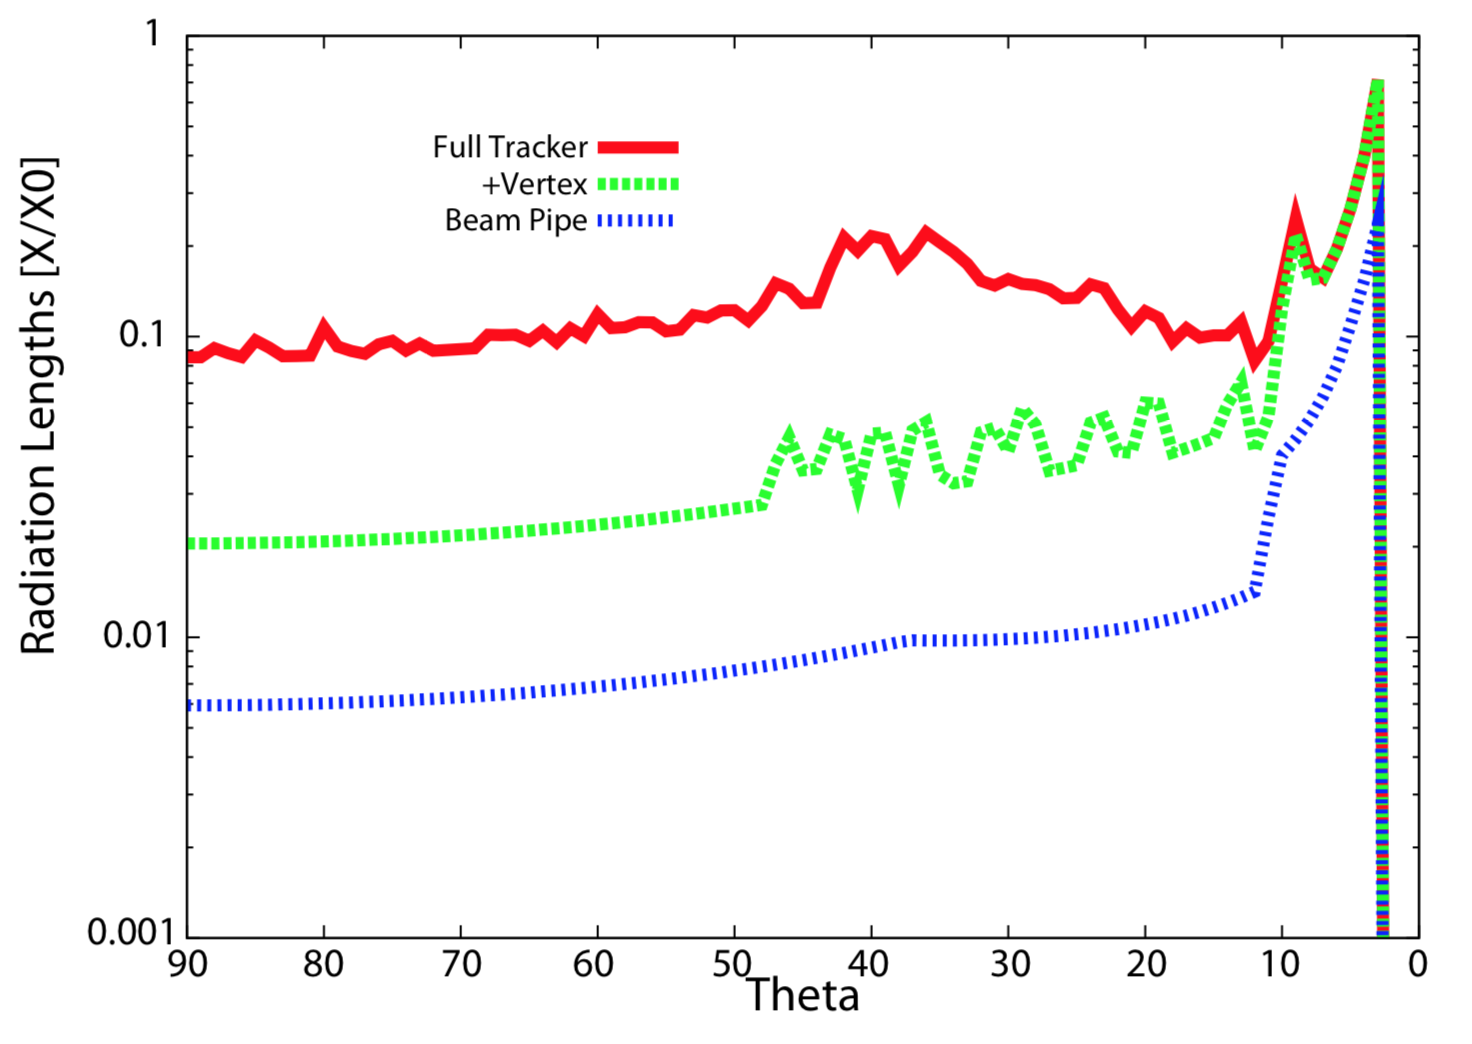
\includegraphics[width=0.80\hsize]{chapters/figures/SiD_material_budget_tracker.png}
\end{center}
\caption{Resulting radiation lengths of the tracking detectors in the \emph{SIDLOI3} simulation model (from~\cite{Behnke:2013lya}).}
\label{fig:sid_mat_budget}
\end{figure}
%%%%%%%%%%%%%%%%%
%%%%%%%%%%%%%%%%
\begin{figure}
\begin{center}
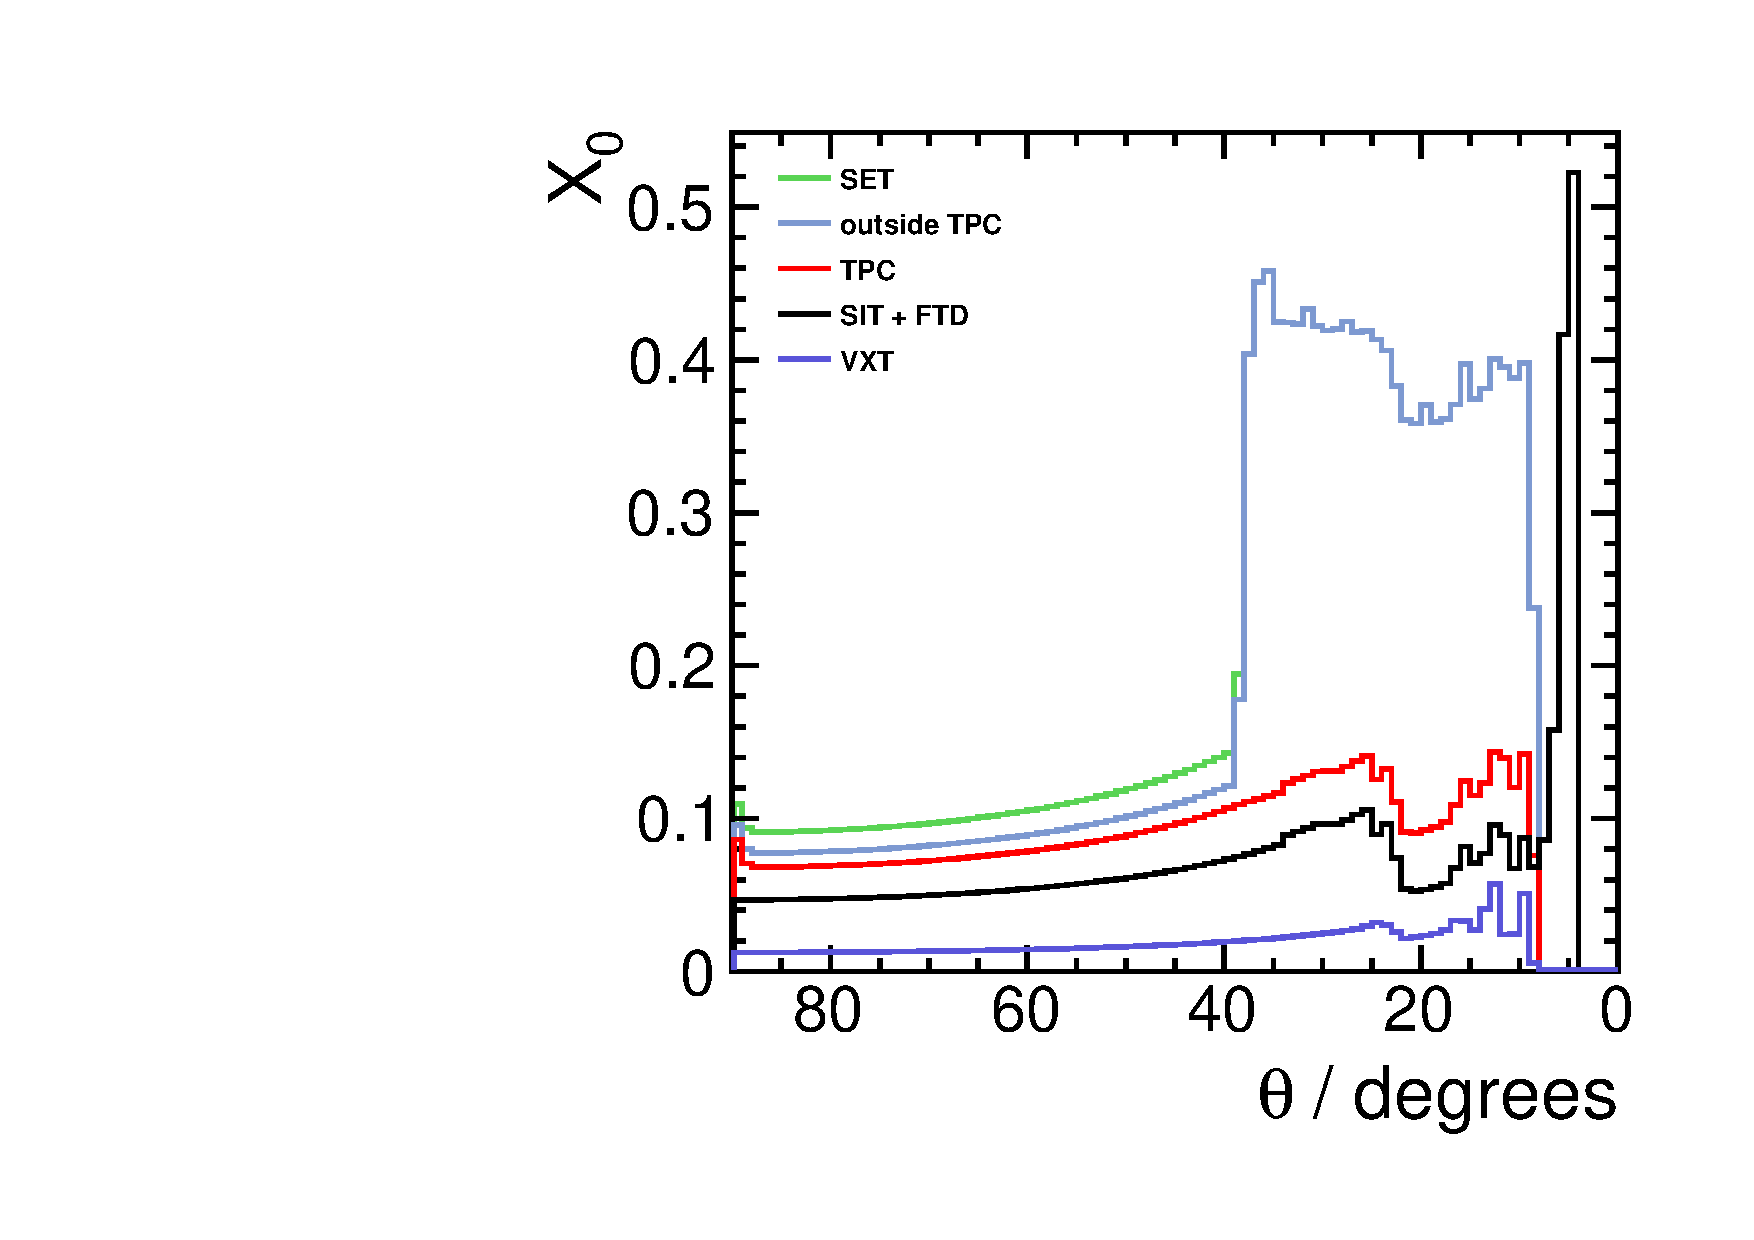
\includegraphics[width=0.80\hsize]{chapters/figures/ILD_material_budget_tracker.pdf}
\end{center}
\caption{Resulting radiation lengths of the tracking detectors in the \emph{ILD\_o1\_v05} simulation model (from~\cite{Behnke:2013lya}).}
\label{fig:ILD_mat_budget}
\end{figure}
%%%%%%%%%%%%%%%%%
The average material budget in the tracking volume of the simulation models is shown in Figures~\ref{fig:sid_mat_budget}
and~\ref{fig:ILD_mat_budget} for SiD and ILD respectively.

Before the two concepts had decided to move to the common geometry description and simulation with DD4hep, they had
implemented their detailed simulation models in Mokka~\cite{MoradeFreitas:2002kj} and slic~\cite{bib:slic}. These models
have been ported into DD4hep preserving all features and dimensions, thus resulting in equivalent simulation results.
Most of the physics analyses in the next sections are based on simulations using these older programs.

The high level of detail in the simulation models as decried above is a key prerequisite for the
realistic understanding of the expected detector performance and the physics reach of the ILC for both detector concepts.

~~~\\
\fix{ here we could add a short paragraph on fast simulations with SGV as this is used in the searches section}
~~~\\

\subsubsection{Digitzation}

The output of the detailed full simulations with Geant4 from ddsim are \emph{SimTrackerHit} and \emph{SimCalorimeterHit} objects,
that store the deposited energy in the sensitive detector elements, such as silicon wafers and calorimeter cells, together with
the position and pointers to the \emph{MCParticle} that created the energy deposition. In the digitization step, carried out in dedicated
Marlin processors, these hits are converted into \emph{TrackerHit} and \emph{CalorimeterHit} objects,
taking into account all relevant effects from the detector and the readout electronics.

The \emph{SimTrackerHits} contain the exact energy-weighted position of the individual energy depositions in a given sensitive
detector element. For silicon strip-and pixel detectors as well as the ILD-TPC, these positions are smeared according to
resolutions that have been established from test beam campaigns for the different sensor technologies, thereby including effects
from charge sharing, clustering and position reconstruction. Table~\ref{tab:ild_trk_res} shows the point resolution parameters used for ILD.



%-----------------------------------------------------------------------
\begin{table}[htbp]
\renewcommand{\arraystretch}{1.25}

\centering\small
\begin{tabular}{llcl}
\hline
 Subdetector &  \multicolumn{3}{c}{ Point Resolution }  \\
\hline
        VTX    &  $ \sigma_{r\phi,z}  $ & $=$ & $ 2.8 \mu\mathrm{m}$   (layer 1)   \\
               &  $ \sigma_{r\phi,z}  $ & $=$ & $ 6.0 \mu\mathrm{m}$   (layer 2)   \\
               &  $ \sigma_{r\phi,z}  $ & $=$ & $ 4.0 \mu\mathrm{m}$   (layers 3-6)   \\


        SIT    &  $ \sigma_{\alpha_{z}}   $ & $=$ & $ 7.0 \mu\mathrm{m}$    \\
               &  $  \alpha_{z}         $ & $=$ & $ \pm 7.0^\circ $ (angle with z-axis)        \\

        SET    &  $ \sigma_{\alpha_{z}}   $ & $=$ & $ 7.0 \mu\mathrm{m}$    \\
               &  $  \alpha_{z}         $ & $=$ & $ \pm 7.0^\circ $ (angle with z-axis)        \\

       FTD     &  $\sigma_{r}$      & $=$ & $ 3.0 \mu\mathrm{m}$    \\
  \emph{Pixel} &  $ \sigma_{r_\perp}$  & $=$ & $ 3.0 \mu\mathrm{m}$    \\

     FTD       &  $ \sigma_{\alpha_r}   $ & $=$ & $ 7.0 \mu\mathrm{m}$    \\
  \emph{Strip} &  $ \alpha_{r}         $ & $=$ & $ \pm 5.0^\circ $ (angle with radial direction)        \\

       TPC    &  $ \sigma^2_{r\phi} $ & $=$ & $ (50^2+900^2\sin^2\phi + \left( (25^2/22)\times (4T/B)^2\sin\theta\right)$ \\
              &                      &     &   $(z/\mathrm{cm}) )\,\mu\mathrm{m}^2$  \\
               &  $ \sigma^2_{z}    $ & $=$ & $ (400^2+80^2\times (z/\mathrm{cm})) \,\mu\mathrm{m}^2 $ \\
               &   \multicolumn{3}{c}{ where $\phi$ and $\theta$ are the azimuthal and} \\
               &   \multicolumn{3}{c}{ polar angle of the track direction } \\
\hline
\end{tabular}
\caption[Simulated ILD tracking point resolutions.]{Effective point resolution as used in the digitization of the ILD tracking detectors.
        \label{tab:ild_trk_res} }
\end{table}
%-----------------------------------------------------------------------

In the TPC hit digitization, simulated hits that are closer than the established double-hit resolution of 2~mm in $r\phi$ and 5~mm
in $z$ are merged into one. For the silicon detectors this treatment is not necessary, due to the expected low occupancies.

The \emph{SimCalorimeterHits} contain the total energy deposited in each calorimeter cell, together with the individual depositions
from the individual Monte Carlo steps. For scintillating calorimeters Birk's Law, resulting in different light yields for different
particles, is already applied during the simulation. Dedicated digitizers take into account effects of non-uniformity of the light yield
for scintillators as well as cross-talk between neighboring channels. The latter is important in particular for the simulation of
(semi)-digital calorimeters using RPCs and is possible due to the availability of the individual simulation steps, containing
the exact position of the energy deposition.

During the calorimeter digitization a two step calibration is applied for every calorimeter type and sampling structure. In a first step
the hits are calibrated to a MIP signal and in a second step, the total energy is calibrated to an absolute value of the
cell energy in $GeV$. This calibration is an iterative procedure, based on the application of the full
\emph{particle flow algorithm }(see next subsection) to single particle events with photons and $K^0$s and thereby
repeatedly adjusting the calibration constants.


  
\subsubsection{Reconstruction}

Tracking: \\

The first step of the event reconstruction consists of identifying the trajectories of charged particles based on the positions of their
energy depositions in the detector (\emph{SimTrackerHits}), typically referred to as \emph{pattern recognition}. In a second step the
kinematic parameters of these trajectories are fitted based on the known equations of motion in a magnetic field and the errors of the
hit positions. Often both steps are carried out together, e.g. by using a Kalman-Filter and simply referred to as \emph{Tracking}.

The tracking packages in iLCSoft is called MarlinTrk and provides a generic tracking-API \emph{IMarlinTrk} and underlying fitting code,
using the Kalman-Filter package \emph{KalTest}~\cite{Li:2013cxa}.
The \emph{IMarlinTrk} interface provides code to iteratively add hits to a track segment,
thereby updating the track parameters, extrapolation of the current track state to the next measurement surface or any given point
in space. It uses LCIO as data model for the Track and TrackState with a \emph{perigee} track parameterization with
track curvature $\omega$, impact parameters $d_0$ and $z_0$ and direction parameters $\phi_0$ and $\rm{tan}(\lambda)$.
A pallete of different pattern recognition algorithms are programmed against \emph{IMarlinTrk} as shown in Fig~\ref{fig:imarlintrk}.
%%%%%%%%%%%%%%%%
\begin{figure}
\begin{center}
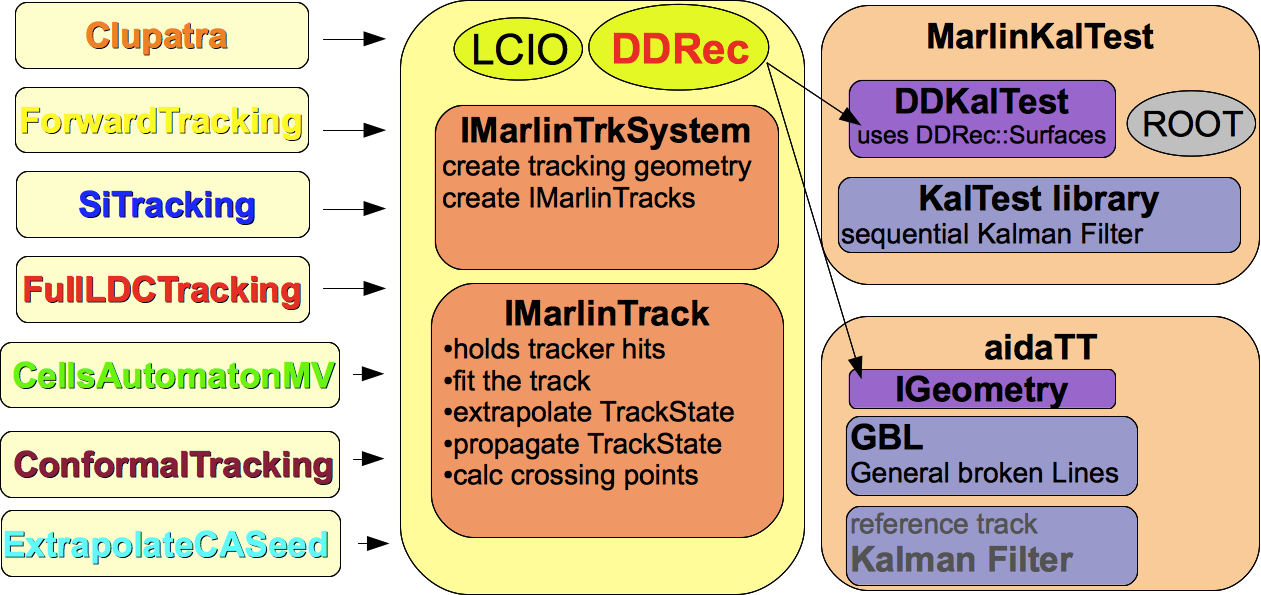
\includegraphics[width=0.80\hsize]{chapters/figures/IMarlinTrk_ddkaltest_new.png}
\end{center}
\caption{Schematic view of the MarlinTrk tracking tools available in iLCSoft. They are based on the LCIO event data model and the
DDRec geometry description.}
\label{fig:imarlintrk}
\end{figure}
%%%%%%%%%%%%%%%%%
ILD uses the following different algorithms in the different parts of the tracking region
(for more details see~\cite{Gaede:2014aza}):

\begin{itemize}
\item SiliconTracking\\
  Algorithm used in the innermost Si-tracking detector VXD and SIT, based an a brute-force triplet seeding followed by
  a road search using the extrapolation to the next layer provided in MarlinTrk.
\item ForwardTracking\\
  Stand alone pattern recognition in the FTD forward tracker using a Cellular-Automaton to find, a possibly large, set of
  track candidates that are reduced to a unique and consistent set through the use of a Hopfield Network.
\item Clupatra\\
  Pattern recognition algorithm for the TPC, based on a topological clustering in the outer TPC pad row layers for seeding,
  followed by a Kalman-Filter based road search inwards.
\item FullLDCTracking\\
  A collection of algorithms for merging track segments from the previous algorithms and assignments of leftover hits followed
  by a final re-fit using a Kalman-Filter.
\end{itemize}

SiD had originally developed their stand alone tracking software in the Java framework \emph{LCSim}~\cite{bib:LCSim}
using a triplet based seeding followed by a road search and a final track fit. More recently SiD has adopted the \emph{ConformalTracking}
algorithm originally developed for CLICdp. It uses a conformal mapping transforming circles going through the origin (IP)
into straight lines which are then identified using a Cellular-Automaton.


\fix{add a short paragraph on DDRec and tracking surfaces here ...}

The resulting tracking efficiencies for the ILD detector are shown as a function of the momentum and
$\rm{cos}(\theta)$ in Fig~\ref{fig:ild_trkeff}.

%%%%%%%%%%%%%%%%
\begin{figure}
  \begin{tabular}[c]{c}
    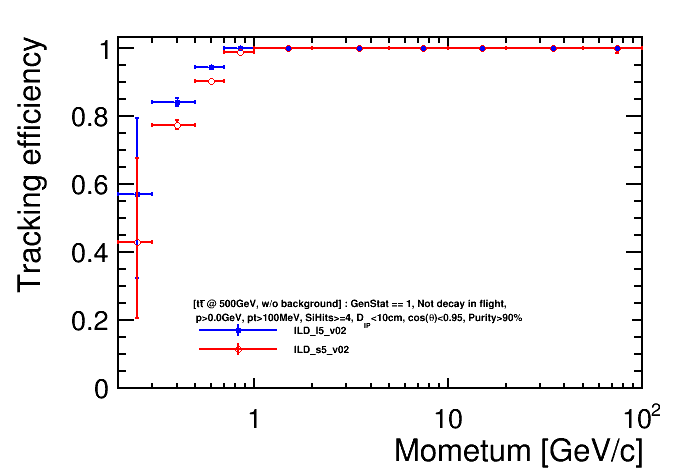
\includegraphics[width=0.95\hsize]{chapters/figures/trkEff_Momentum_ttbar_ILD_ls5_v02_publish2.png} \\
    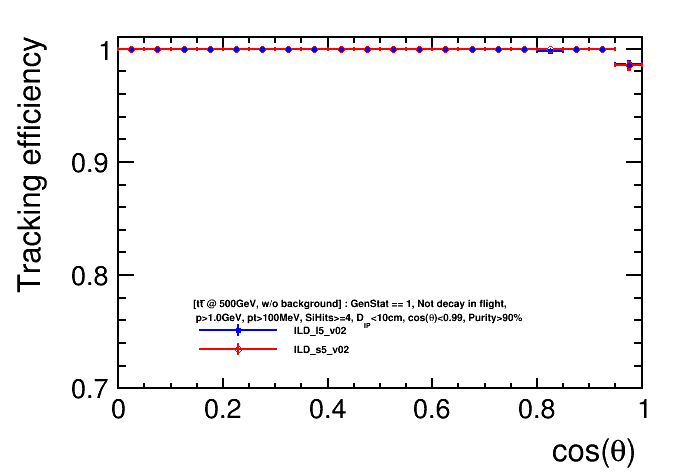
\includegraphics[width=0.95\hsize]{chapters/figures/trkEff_theta_ttbar_ILD_ls5_v02_publish1.png}
\end{tabular}
  \caption{Tracking efficiency for the ILD detector as a function of momentum (upper) and $\rm{cos}(\theta)$ (lower).
    Blue: the standard ILD detector, Red: an alternative smaller version of ILD. \fix{make nicer plots}
of ILD.}
\label{fig:ild_trkeff}
\end{figure}
%%%%%%%%%%%%%%%%%

The normalised transverse momentum resolution $\sigma(1/p_T)$ for single-muon events the SiD detector model is shown in
Fig~\ref{fig:sid_mom_res} together with fits using the parameterisation:

\begin{equation}
  \frac{\sigma(p_T)}{p^2_T} = a~\oplus~\frac{b}{p~\rm{sin}\theta}     \label{eq:trk_res_param}
\end{equation}

%%%%%%%%%%%%%%%%
\begin{figure}
\begin{center}
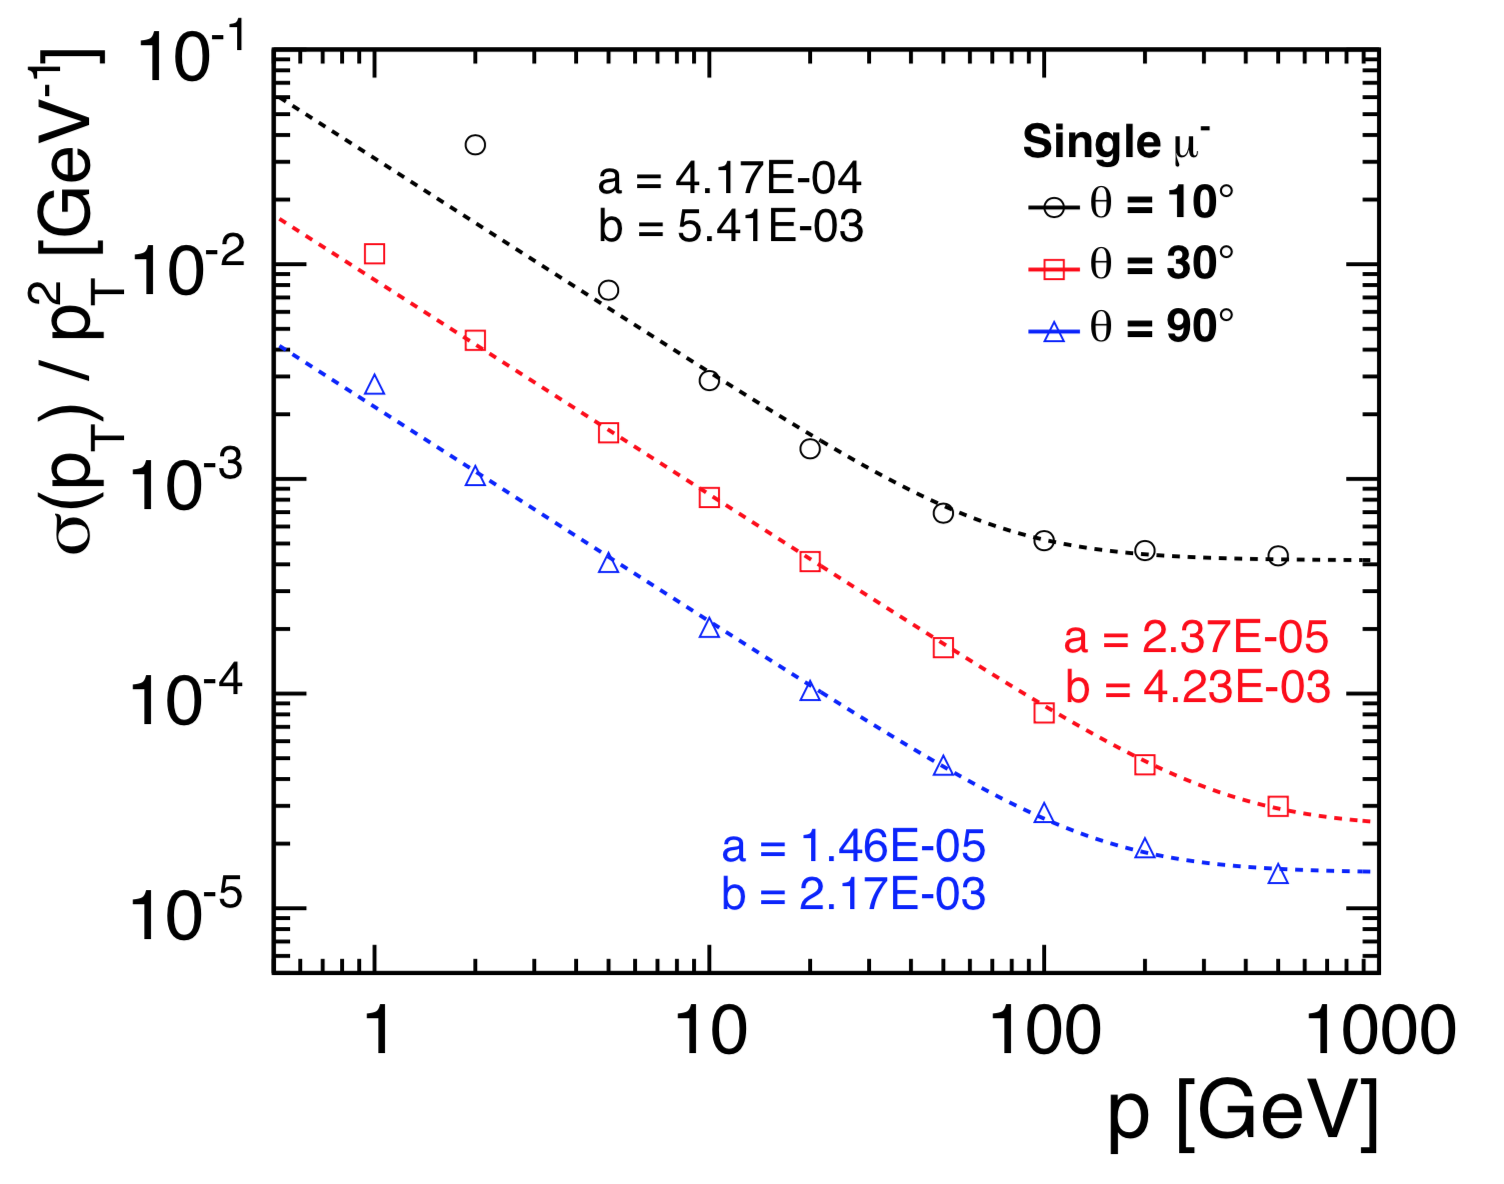
\includegraphics[width=0.95\hsize]{chapters/figures/SiD_momentum_resolution.png}
\end{center}
\caption{Normalised transverse momentum resolution for single-muon events as function of momentum
  in the \emph{SIDLOI3} simulation model (from~\cite{Behnke:2013lya}). The dashed lines are fits to the data points according
  to eq.~\ref{eq:trk_res_param}.}
\label{fig:sid_mom_res}
\end{figure}
%%%%%%%%%%%%%%%%%

Comparable results are obtained for ILD and both detector concepts achieve their design goals for the momentum resolution of
$\sigma(p_T)/P^2_T  < 2 \times 10^{-5} \rm{GeV}^{-1}$ for high momentum central tracks.

%%%%%%%%%%%%%%%%
\begin{figure}
\begin{center}
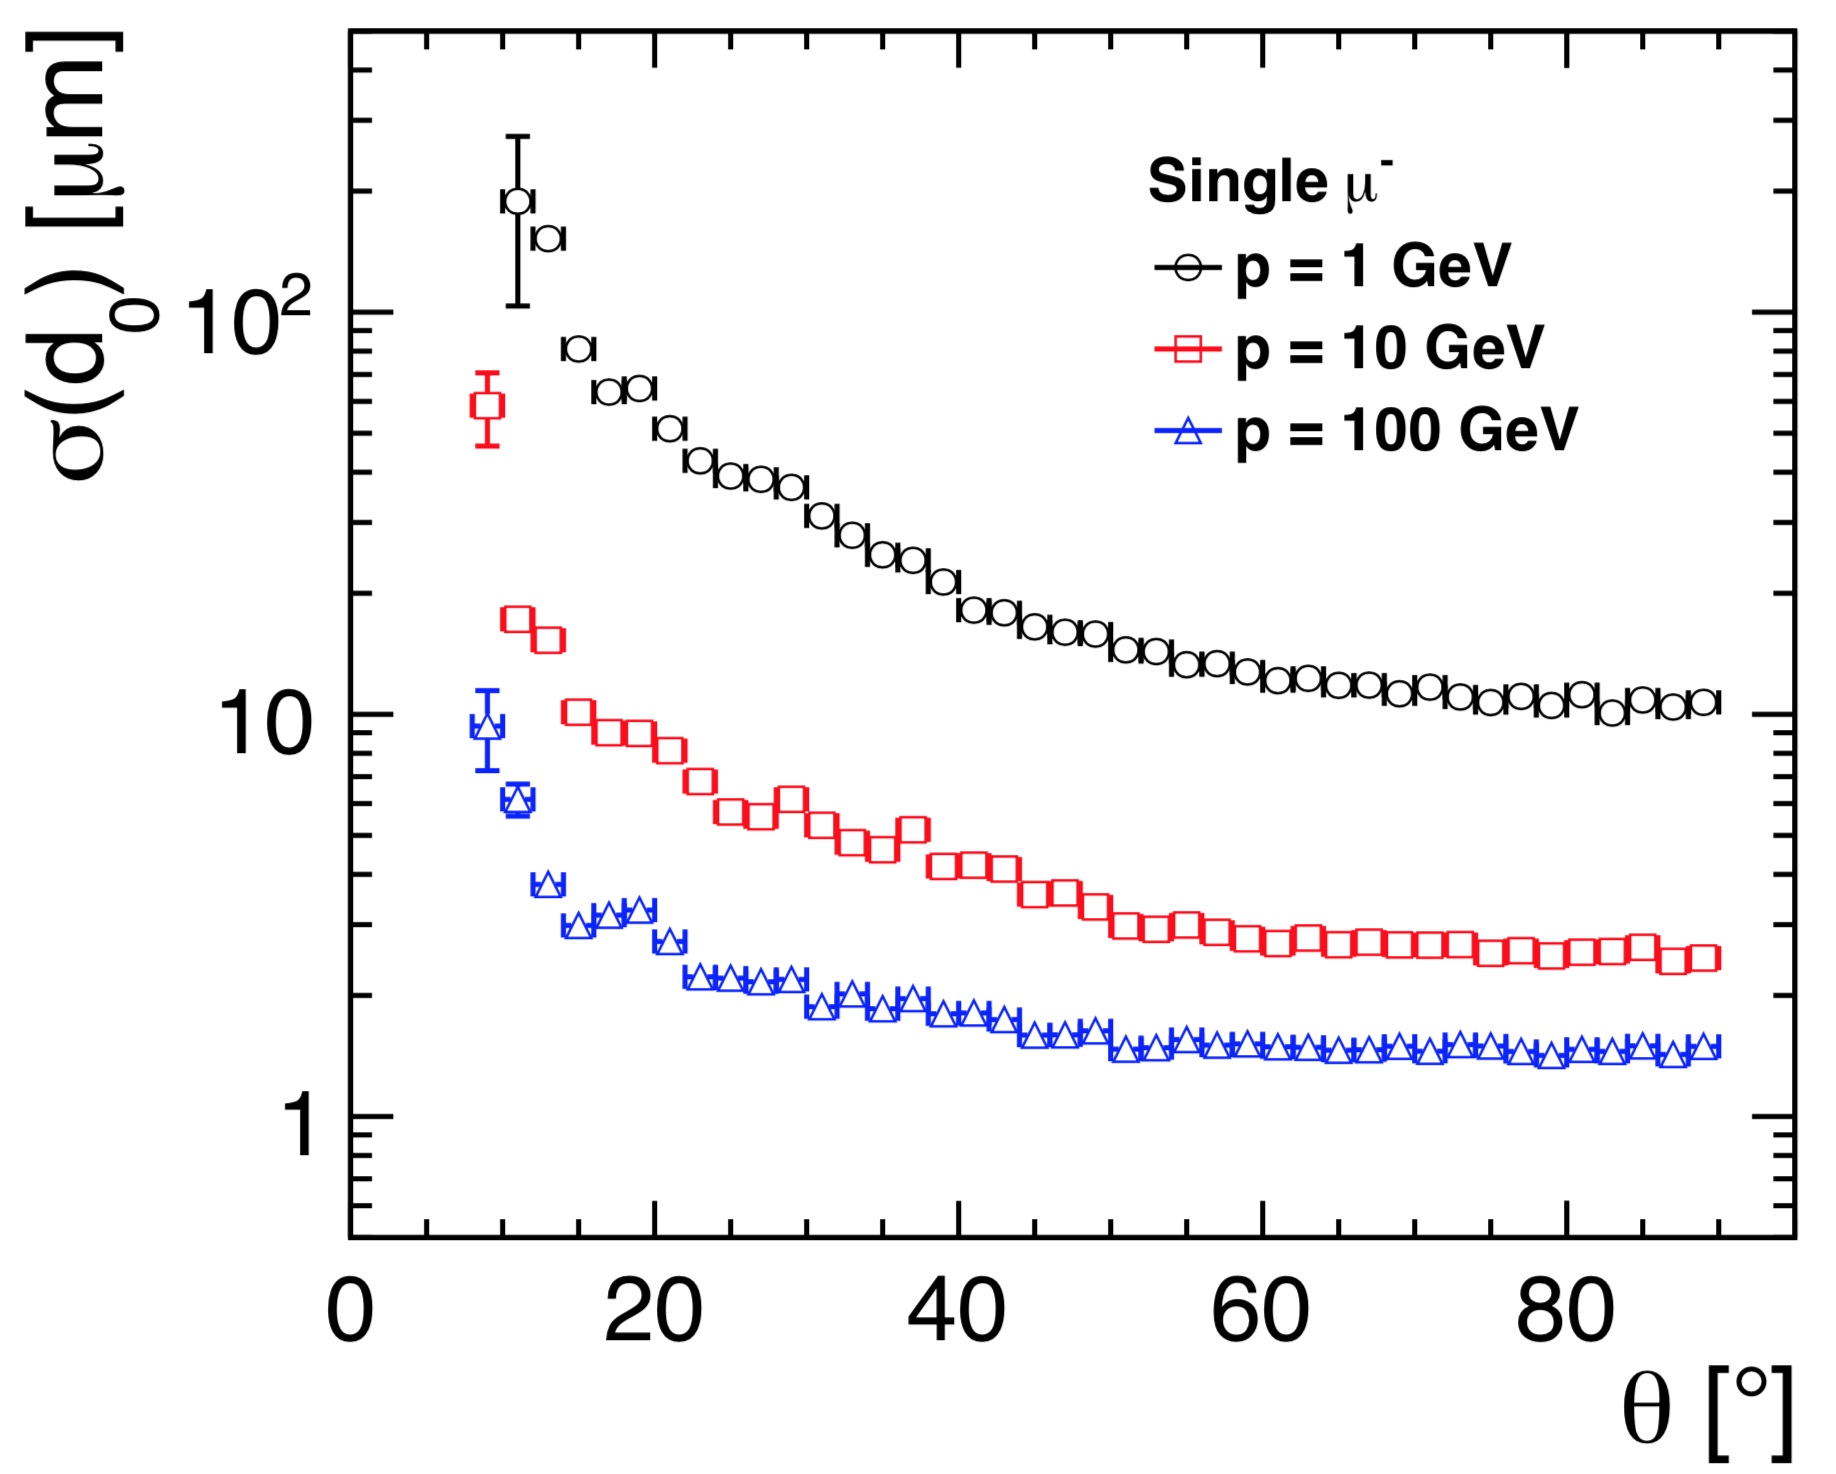
\includegraphics[width=0.85\hsize]{chapters/figures/SiD_D0_resolution.png}
\end{center}
\caption{Impact parameter resolution $\sigma(d_0)$ for single-muon events as function of polar angle
  in the \emph{SIDLOI3} simulation model (from~\cite{Behnke:2013lya}).} 
\label{fig:sid_d0_res}
\end{figure}
%%%%%%%%%%%%%%%%%

The impact paramter resolution as a function of polar angle for single-muon events in SiD is shown in Fig~\ref{fig:sid_d0_res} for
different particle momenta. A resolution of a few $\mu\rm{m}$ is achieved for high mometum tracks over a large range of the polar
angle down to $\sim 20^{o}$.


The tracking software is completed with a dedicated processors for the identification and reconstruction of kinks and $V_0$s.
Tracks with kinks can arise from bremsstrahlung, typically for electrons, or a large angle deflection due to multiple scattering.
$V_0$s are almost exclusively decays of $K^0_s$ and $\Lambda^0$ as well as gamma conversions.

%----------------------------------------------
~~~\\
Particle Flow: \\

The \emph{particle flow algorithm} (PFA) aims at reconstructing every individual particle created in the event in order
to take the best available measurement for the given particle type, i.e.:
\begin{itemize}
\item charged particles\\
  using the momentum measured in the tracking detectors with the excellent resolution described  above
\item photons\\
  measured in the Ecal with an energy resolution of $\sigma(E)/E \sim  11\% / \sqrt{(E/\rm{GeV})}$ \fix{is this the correct number?}
\item neutral hadrons\\
  measured predominantly in the Hcal\footnote{hadronic showers often start in the Ecal and might extend into the Muon system -
    this is taken into account in PandorPFA} with an energy resolution of $\sigma(E)/E \sim  50\% / \sqrt{(E/\rm{GeV})}$ \fix{is this the correct number?} 
\end{itemize}

The best jet energy measurement in hadronic events would be achieved if the above algorithm would work perfectly. However in reality
there is always confusion in the assignment of individual \emph{CalorimeterHits} to Clusters and showers as well as in the assignment
of tracks to clusters. This effect is demonstrated in Fig~\ref{fig:pandorapfa_perfect} for PandoraPFA~\cite{Marshall:2015rfa}, the
implementation of PFA available in iLCSoft that is used by both detector concepts.

%%%%%%%%%%%%%%%%
\begin{figure}
\begin{center}
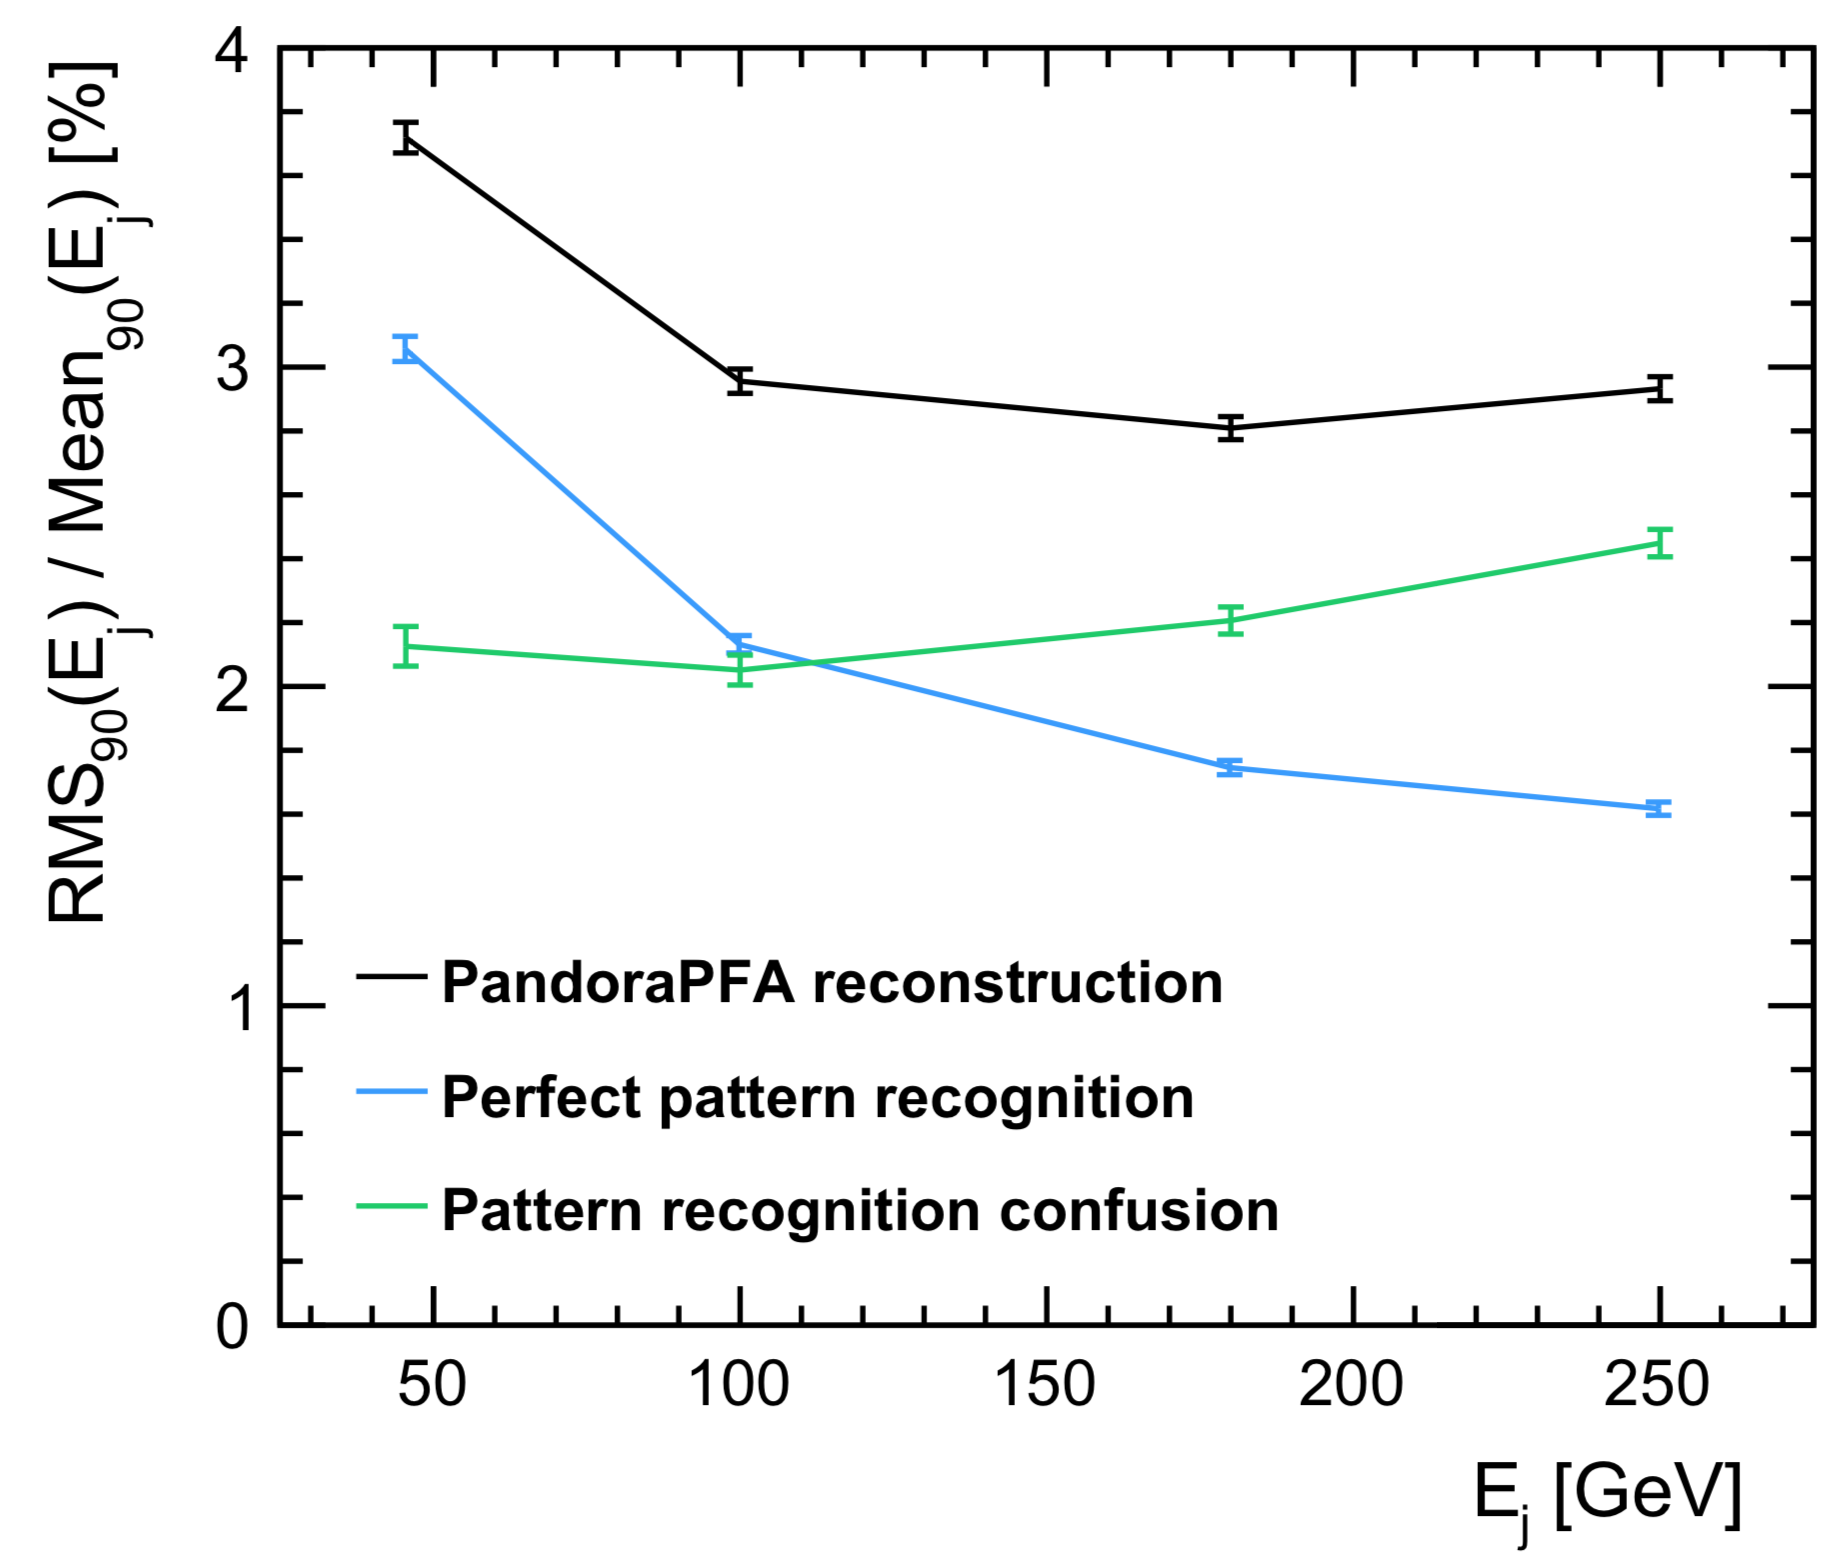
\includegraphics[width=0.85\hsize]{chapters/figures/pandorapfa_perfect.png}
\end{center}
\caption{Jet energy resolution for $Z'$ events as a function of the jet energy in a realistic detector for PandoraPFA.
  Also shown are the effect of \emph{confusion} and the result assuming \emph{perfect PFA} (from~\cite{Marshall:2015rfa}).} 
\label{fig:pandorapfa_perfect}
\end{figure}
%%%%%%%%%%%%%%%%%

The input to PandoraPFA are collections of Tracks, Kinks, $V0$s and collections of all digitized \emph{CalorimeterHits} together with
some geometrical information retrieved from DDRec.
Following~\cite{Marshall:2015rfa} the main steps of the algorithm are:

\begin{itemize}
\item \emph{CalorimeterHits} are clustered using a simple cone-based algorithm, seeded either from isolated hits in the first calorimeter
  layers or by the projection of Tracks to the front face of the Ecal.

\item the clustering algorithm is configured to prefer splitting of clusters rather than risking to falsly merge particles into single
  clusters.

\item Clusters are associated to Tracks based on topological (position and direction) and kinematic (momentum and energy) consistency.
  In case of significant discrepancies a re-clusering is initiated.

\item Clusters without associated Tracks are transformed into neutral \emph{ReconstructedParticles} unless they can be more likely
  interpreted as fragments of charged particles.
  
\item consistent Track-Cluster combinations are transformed into charged \emph{ReconstructedParticles}
  
\item particle identification plugins are applied to label specific particle types, such as photons, electrons and muons.

\item a dedicated weighting procedure known as \emph{software compensation} is applied to the hits inside a cluster in order
  to equalize hadronic and electromagnetic shower components 
  
\end{itemize}


The final output collection of PandoraPFA is called ``PandoraPFOs'' and represents the final output of the \emph{Reconstruction}
process. This collection is either directly used for physics analyses or serves as input to higher-level reconstruction
algorithms where necessary.

Fig~\ref{fig:ild_jer_jes} shows the jet energy resolution and jet energy scale that is achieved for two variants of the ILD detector
for a dedicated event sample of hadronic $Z\rightarrow u,d,s$ events.
The jet energy resolution is evaluated using $RMS_{90}(E)$, the root mean square of the energy of the central 90\% of the events.
The restriction to $u,d,s$ quarks is chosen to focus on  the detector and PFA performance without the extra complication of missing
energy due to neutrinos.

%%%%%%%%%%%%%%%%
\begin{figure}
  \begin{tabular}[c]{c}
    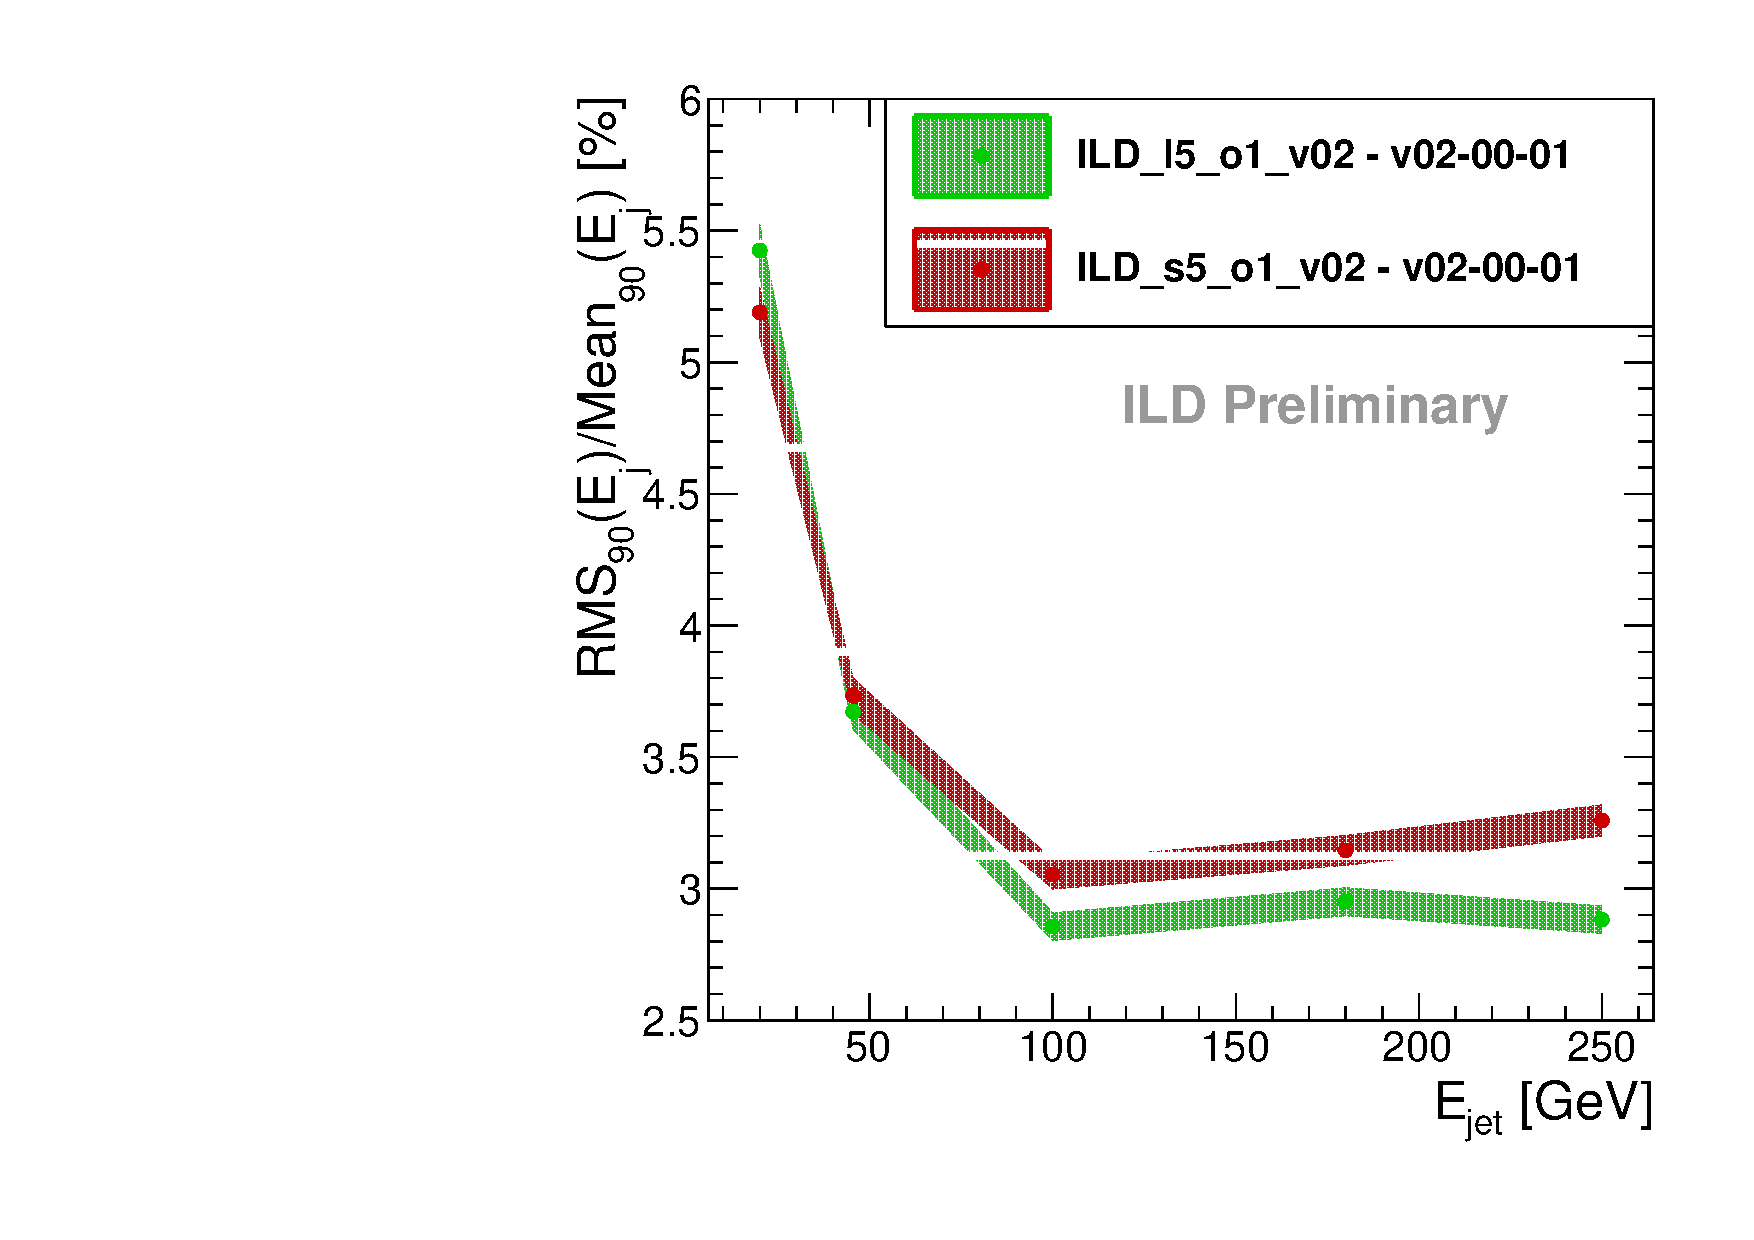
\includegraphics[width=0.85\hsize]{chapters/figures/JERLargeSmall_v02-00-01.pdf} \\
    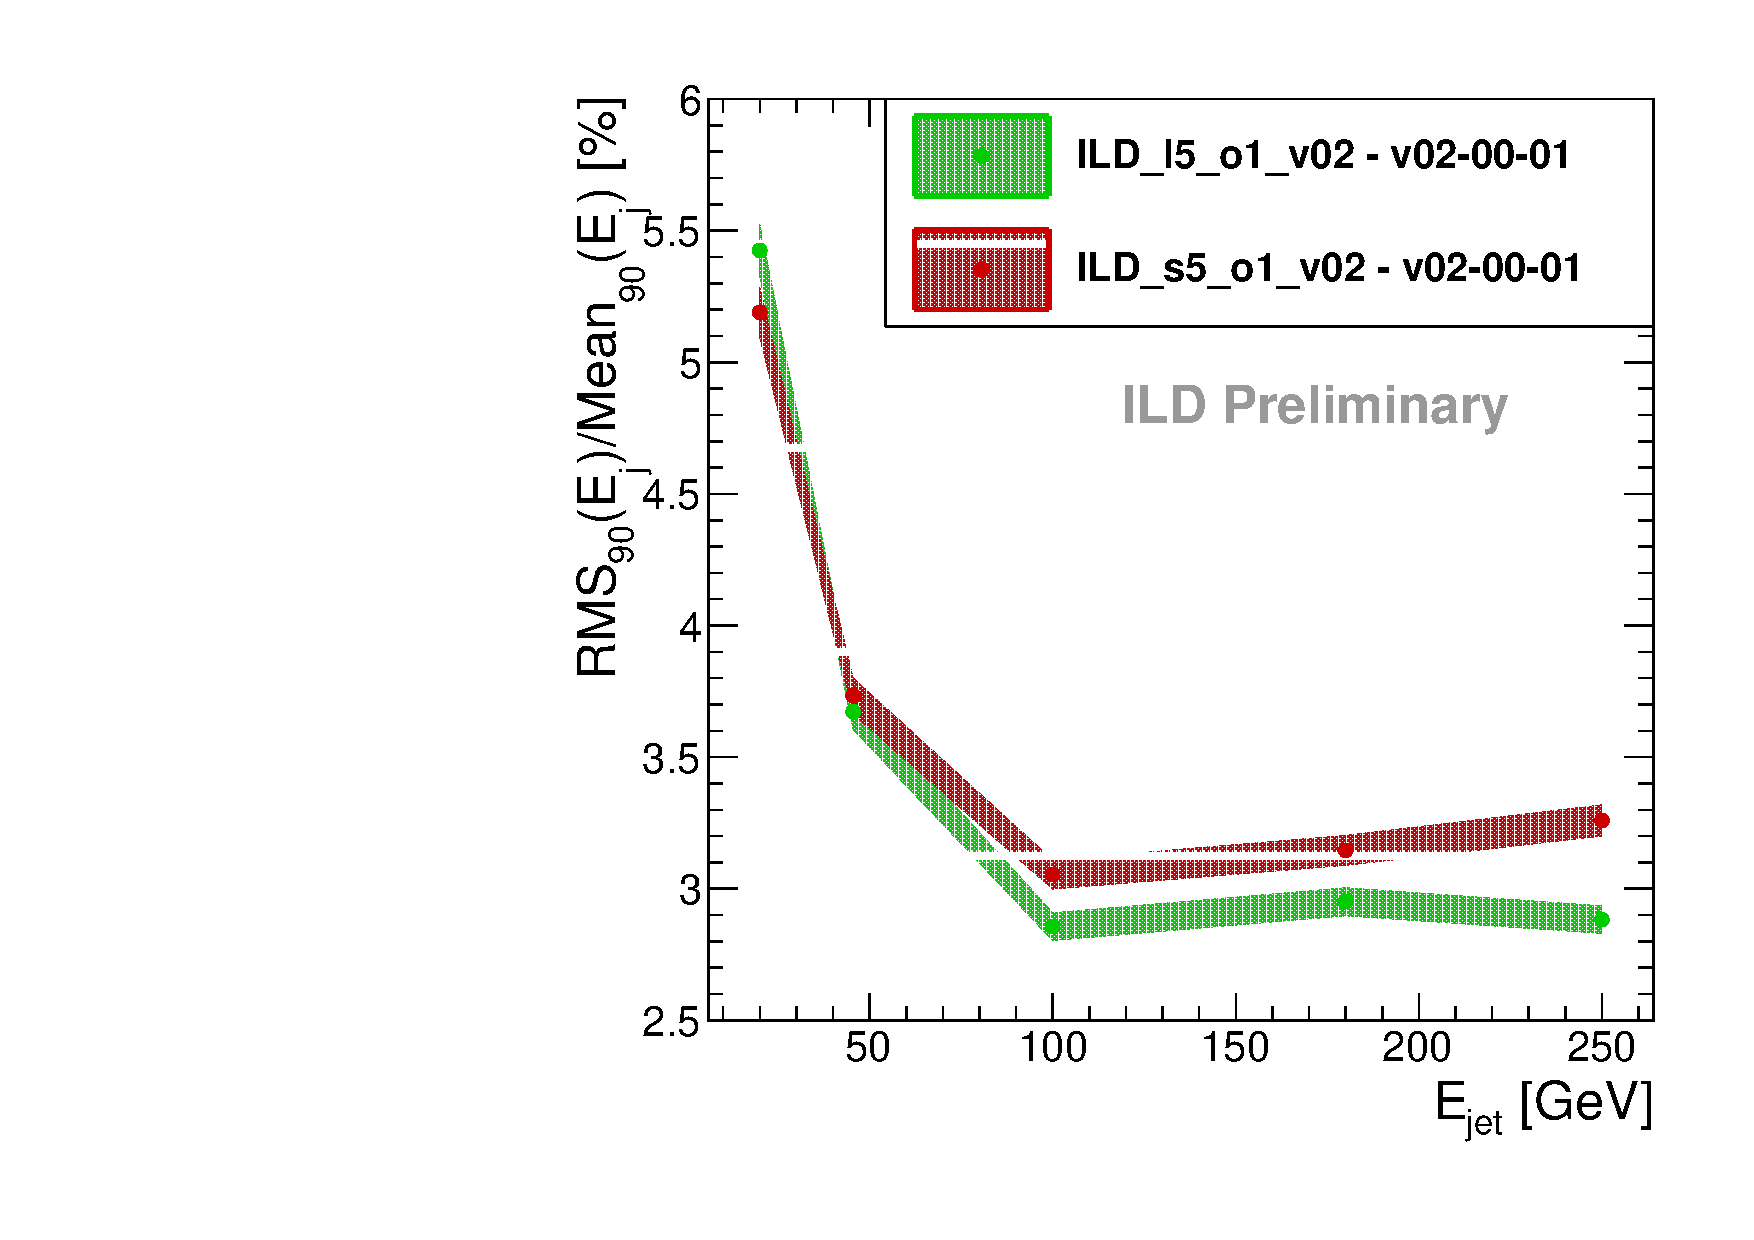
\includegraphics[width=0.85\hsize]{chapters/figures/JESLargeSmall_v02-00-01.pdf}
  \end{tabular}
  \caption{Upper: Jet energy resolution for $Z\rightarrow u,d,s$ events as a function of the jet energy in the standard ILD simulation model
    (\emph{ILD\_l5\_v02}) and an alternative smaller version of ILD  (\emph{ILD\_s5\_v02}).
    Lower: The resulting jet energy scale for the same models and events.} 
\label{fig:ild_jer_jes}
\end{figure}
%%%%%%%%%%%%%%%%%


  

\subsubsection{High-Level Reconstruction}

After having reconstructed all the individual particles in the event, the next step in the processing is the reconstruction of
primary and secondary vertices. This is carried out in iLCSoft with the LCFIPlus~\cite{Suehara:2015ura} package that is also used
for the tagging of heavy flavor jets.

The primary vertex of the event is found in a tear-down procedure. First an initial vertex is fitted by a $\chi^2$-minimization using
all charged tracks in the event and a constraint from the expected beam spot
$(\sigma_x=516~\rm{nm}, \sigma_y=7.7~\rm{nm},\sigma_z \sim 200~\mu\rm{m}~~\rm{at}~~~E_{cms}=250~\rm{GeV})$.
Then all tracks with a $\chi^2$-contribution larger than a given threshold value are removed.

In a second step LCFIPlus tries to identify secondary vertices, starting out from forming all possible track-pairs from tracks not
used in the primary vertex. The pairs have to fulfill suitable requirements with respect to their invariant mass, momentum direction
and $\chi^2$. $V^0$s are excluded from these initial pairs. Secondary vertices are then formed using so far leftover tracks in
an iterative procedure and eventually adding compatible tracks originally used in the primary vertex.

Secondary vertices and optionally isolated Leptons can be used by LCFIPlus for jet clustering, aiming at high efficiency for correctly identifying
heavy flavor jets. The actual jet clustering is then performed by using a cone-based clustering with a Durham-like algorithm.
Alternatively users can use $k_T$ jet clustering algorithms from the Fastjet~\cite{Cacciari:2006sm} that is interfaced to Marlin in a dedicated
package MarlinFastJet.

LCFIPlus also provides algorithms for jet flavor tagging using boosted decision trees (BDTs) based on suitable variables from tracks and vertices.
Fig~\ref{fig:sid_flavor_tag} shows the mis-identification efficiency for jets from light quarks and c-quarks as a function of the b-tagging efficiency
for the SiD detector using LCFIPlus.

%%%%%%%%%%%%%%%%
\begin{figure}
\begin{center}
\includegraphics[width=0.9\hsize]{chapters/figures/SiD_flavor_tag.png}
\end{center}
\caption{Mis-identification efficiency of light quark jets (red points) and charm jets (green points) as beauty jets versus beauty identification efficiency in
  di-jets events at $\sqrt{s} = 91~\rm{GeV}$ (from~\cite{Behnke:2013lya}).} 
\label{fig:sid_flavor_tag}
\end{figure}
%%%%%%%%%%%%%%%%%


There is a large palette of additional high level reconstruction algorithms available in iLCSoft addressing the needs for physics analyses, e.g.
\begin{itemize}
\item particle identification using dE/dx, shower shapes and multi-variate methods
\item $\gamma\gamma$-finders for the identification of $\pi^0$s and $\eta$s
\item reconstructed particle to Monte-Carlo truth linker for cross checking analysis and reconstruction efficiencies
\item tools for jet clustering using Monte-Carlo truth information
\item processors for the computation of various event shapes 
\end{itemize}




\subsection{Computing}

An initial computing concept for the ILC, including a first estimate of the required resources, has been developed by the LCC Software and Computing Group.

\subsubsection{Computing Concept}

The foreseen computing concept follows in general terms that of the current LHC experiments and Belle~II, with a strong on-site computing center complemented by large
Grid-based computing resources distributed around the world. This concept is schematically shown in Fig~\ref{fig:computing_scheme}.

%%%%%%%%%%%%%%%%
\begin{figure*}
\begin{center}
\includegraphics[width=0.6\hsize]{chapters/figures/ILC_computing_scheme.png}
\end{center}
\caption{Computing concept foreseen for the ILC, distributed over on-site computing at the interaction region, the main campus and Grid-like offline computing.}
\label{fig:computing_scheme}
\end{figure*}
%%%%%%%%%%%%%%%%%

Due to the much lower event rates at the ILC compared to the LHC, we will be
able to run in an un-triggered mode in which  collision data from every bunch crossing will be recorded. At the experimental site, we require only limited computing
resources for online monitoring, QA, and data-buffering for a few days.

Prompt reconstruction, event building, and filtering of the interesting collisions will be performed at the main ILC campus.
A few percent of the initial data will be distributed to major participating Grid sites in the world for further skimming and final redistribution for physics
analysis. A copy of the raw data from all bunch crossings will be kept to allow  for future searches for new exotic signatures. 


\subsubsection{Resource Estimate}

Based on our detailed physics and background simulations,  we estimate the total raw data rate of the ILC to be $\sim$1.5GB/s.

The total estimated storage needs will be a few tens of PB/y.
The computing power needed for simulation, reconstruction, and analysis will be a few hundred kHepSpec06.
Given that these numbers are already smaller than what is now
needed by the LHC experiments, and given an expected annual increase
of 15\% and 20\%, respectively, for storage and CPU
at flat budget, we expect the overall computing costs for the ILC
will be more than an order of magnitude smaller than those for the LHC.

\fix{extend this with a bit more detail, e.g. a small table with the main parameters relevant for the estimate ...}





\section{\label{sec:higgs}Physics Simulations: Higgs
%and Electroweak
}


  20 pages Tian + J. List
  
  % Higgs simulation and experiementation section

%  should also include WW ?  yes!

\subsection{Analyses of four-fermion final states} 
\input{chapters/fullsim_4f.tex}

\subsection{Analyses of two-fermion final states}
\input{chapters/fullsim_2f.tex}

\subsection{Higgs analyses}
\input{chapters/fullsim_higgs.tex}


\subsection{Comparison of the ILC Higgs capability with 
HL-LHC projections}

It is appropriate to compare the capabilities of the ILC for precision
Higgs measurement to those of the HL-LHC.  Since the ILC is planned as
an expensive new accelerator project, it should be justified on the
basis that it will qualitatively advance our knowledge of the Higgs
boson over what is possible from the LHC in its high luminosity stage.  
This section will present several such comparisons.

The goal of the ILC is not simply to achieve a high degree of
precision in the measurement of Higgs boson couplings; it is to
discover deviations of the Higgs boson couplings from their Standard
Model predictions and to demonstrate those deviations with a high
degree of confidence.  The strengths of the ILC program are the
 following:
\begin{enumerate}
\item The ILC will report the properties of the Higgs boson in a
  highly model-independent framework.   Our estimate for the ILC capabilities
  are based on an effective field theory (EFT) model that includes
 {\underline{all}}\ dimension-6 operators that appear in the relevant physics
  cross sections at the tree level  (16 operators in all).   Our model
  also includes 2 further parameters to account for possible invisible
  and exotic Higgs decays.  The errors in this model due to
  unaccounted terms are percent-level corrections relative to the new
  physics effects already included in the model.   The analysis includes a
  high-precision determination of the Higgs boson total width. 
 Thus, the ILC will be able to measure  the full array of Higgs 
boson decays and to detect and quantify anomalies in any aspect of this behavior.
\item  For the Higgs boson couplings to $ZZ$, $WW$, and $b\bar b$, 
the ILC will achieve 1\% precision in its initial 250 GeV
  stage.   This is the
 level deemed necessary to be sensitive to the typical predictions 
of the effects of new physics models on the Higgs boson couplings.
\item  If  anomalies are  discovered in the ILC 
250 GeV program, these
  anomalies can be confirmed with an independent data set by
  increasing the energy of the ILC to 500 GeV.   This second energy
  stage will improve the precision of the ILC 
determinations by about a factor of 2.  
\item The ILC, with Higgs bosons tagged by recoil against a $Z$ boson
  and with no trigger requirements, will be able to observe directly
  all manner of exotic Higgs boson decays that might be produced by
Higgs couplings  to  light, weakly coupled  particles.
\end{enumerate}
All of these features go qualitatively beyond what is possible at the 
LHC, or at any hadron collider.

Beyond these conceptual improvements, we can compare the ILC
capabilities quantitatively to the projections released in the HL-LHC
Yellow Report \cite{YR}.   This comparison is given in
Table~\ref{tab:ILCLHC}.   It is not so straightforward to give a
direct apples-to-apples comparison to the estimates presented in the
Yellow Report.    The HL-LHC projections are reported in two
scenarios.  Scenario 1 (S1) is a projection based on our current
understanding of Higgs boson analyses, adding the increased data
available from the HL-LHC.   Scenario 2 (S2) assumes that the current
analyses can be improved by dividing the current theoretical
systematic errors by 2 and dividing the current experimental
systematic errors by $\sqrt{N}$, a factor of 6.   The latter
assumption, in particular, leads to very significant reductions in the
uncertainties.   S2 is intended to model the progress that the LHC
experiments have made in improving their understanding through actual
experience working with the data.  Still, ``past performance is not a 
guarantee of  future results''.

In spirit of the HL-LHC projections, we present multiple estimates of the ILC
capabilities at 250 GeV  in Table~\ref{tab:ILCLHC}.   We consider
these in turn.   The analysis labelled S1* in the table is based
on the highly model-independent framework described in item 1 above.
It is based on 2 ab$^{-1}$ of ILC data at 250~GeV on the reaction
$\ee\to hZ$.   To fix certain EFT operator coefficients, it also makes
use of data on $\ee \to W^+W^-$ at 250~GeV, as well as precision
electroweak measurements.   The analysis also includes
information from LHC that should be available from the 
HL-LHC results.  The LHC measurement of the ratio of the $\gamma\gamma$ and 
$ZZ^*$ branching ratios, which should be almost free of systematic
errors from the Higgs production process, plays an important role, and
the LHC measurments of the 
$\mu^+\mu^-$ and $Z\gamma$ branching ratios are used to constrain
those modes. 
The estimates of measurement errors
for the various ILC observables  are obtained as the result of  full
simulation studies using the ILD and SiD detector models.   The table
of input measurements is 
presented in some detail in Appendix A of \cite{Barklow:2017suo}. 


%%%%%%%%%%%%%%%%
\begin{figure}
\begin{center}
\includegraphics[width=0.85\hsize]{chapters/figures/ModelindepSummary.pdf}
\caption{Projected Higgs boson coupling uncertainties for the ILC
  program at 250~GeV and an energy upgrade to 500~GeV, using the
  highly model-independent analysis presented in \cite{Fujii:2017vwa}. This
  analysis makes use of  data on $\ee\to W^+W^-$ in addition to Higgs
  boson observables and also incorporates projected LHC results, as described
  in the text.  These
values correspond to the  scenario S1* in Table~\ref{tab:ILCLHC}.}
\label{fig:ILCmodelindep}
\end{center}
\end{figure}
%%%%%%%%%%%%%%%%%%%%%%%%%%%%%%%%%%%%%%%%%%%%%%%%%%%%%%%%%%%%%%
%%%%%%%%%%%%%%%%
\begin{figure}
\begin{center}
\includegraphics[width=0.85\hsize]{chapters/figures/ModeldepSummary.pdf}
\caption{Projected Higgs boson coupling uncertainties for the LHC and
  ILC
using the model-dependent assumptions appropriate to the LHC Higgs
coupling fit.   The
dark and light red bars represent the projections in the scenarios S1
and S2 presented in  \cite{YR}.    The dark and light green bars represent the
projections in the ILC scenarios S1 and S2 described in the
text.  The dark and light blue bars show the projections for scenarios S1 and S2
when
data from the 500~GeV run of the ILC is included.}
 \label{fig:ILCLHC}
\end{center}
\end{figure}
%%%%%%%%%%%%%%%%%%%%%%%%%%%%%%%%%%%%%%%%%%%%%%%%%%%%%%%%%%%%%%


The LHC S1 estimates do not assume such a model-independent framework.
Among the many model-dependent assumptions in the LHC  analyses, two are
particularly important. They  assume  that the Higgs boson has no decay
modes beyond those predicted in the SM, and they  assume that the Higgs
boson couplings to $WW$ and $ZZ$ are modified only by a rescaling.  In
the ILC EFT analysis, each of these these couplings depends on two
independent constants, called $\eta_{W,Z}$ and $\zeta_{W,Z}$ in
\cite{Barklow:2017suo}.   We can redo the ILC EFT analysis
adding these two assumptions, that is, assuming no
Beyond-Standard-Model decays and assuming $\zeta_{W} = \zeta_Z = 0$.
This gives the uncertainty estimates listed for ILC  in the column S1
in Table~\ref{tab:ILCLHC}.   We consider the comparison of the S1
uncertainties the most direct comparison of the capabilities of  LHC
alone with results of adding the ILC dataset. 
  We emphasize that the S1 analysis is 
simply a recast of the S1* estimates; the ILC inputs are based just 
as firmly in our full-simulation results.

%%%%%%%%%%%%%%%%%%%%%%%%%%%%%%%%%%%%%%%%%%%%5
\begin{table}[!htbp]
\begin{center}
\begin{tabular}{lccccc}
   coupling     &  current  &    S1*     &     S1     &    S2*   &   S2   \\ \hline 
$hZZ$ - LHC  &     11.      &        &       2.5   &        &  1.7 \\ 
\phantom{$hZZ$} - ILC 250 &      &   0.67  &  0.46   &   0.64   &  0.36 \\ 
\phantom{$hZZ$} - ILC 500&      &   0.35  &  0.20  &  0.32   & 0.18 \\ 
 \hline 
$hWW$ - LHC  &    15.       &        &    3.0     &        &  2.1 \\ 
\phantom{$hWW$} - ILC 250 &      &   0.66 &  0.44   &   0.62  &  0.36 \\ 
 \phantom{$hWW$} - ILC 500 &      &   0.34 &  0.19   &  0.32 & 0.18 \\ 
   \hline 
$hbb$ - LHC  &    29.       &        &          5.5   &        & 4.0 \\ 
\phantom{$hbb$} - ILC 250 &      &  1.1  & 0.83   &   0.90   &  0.68 \\ 
\phantom{$hbb$} - ILC 500 &      &  0.58  & 0.42   &  0.48  &  0.36 \\ 
 \hline 
$h\tau\tau$ - LHC  &    17.       &        &              3.6  &        & 2.8 \\ 
\phantom{$h\tau\tau$} - ILC 250 &      &  1.2  &  0.98   &   1.0  &  0.86 \\ 
\phantom{$h\tau\tau$} - ILC 500 &      &  0.74  &  0.63   &  0.67   & 0.59 \\ 
    \hline 
$hgg$ - LHC  &     15.      &        &            4.0   &        &
                2.8   \\ 
\phantom{$hgg$} - ILC 250 &      &  1.7  &  1.6   &   1.3   &  1.2 \\ 
 \phantom{$hgg$} - ILC 500 &      &  0.95  &  0.91   &  0.74  & 0.70 \\ 
\hline 
$hcc$ - LHC  &    -       &        &           -  &        &  - \\ 
\phantom{$hcc$} - ILC 250 &      &   1.9  &  1.8   &   1.4  &  1.3 \\ 
\phantom{$hcc$} - ILC 500 &      &  1.2  &  1.1   &   0.9  &  0.84 \\ 
    \hline 
$h\gamma\gamma$ - LHC  &    15.       &        &         3.6  &        & 2.8 \\ 
\phantom{$h\gamma\gamma$} - ILC 250  &      &   1.2  &  1.1  &   1.2   &  1.0\\ 
 \phantom{$h\gamma\gamma$} - ILC 500  &      &   1.0  &  0.99 &   1.0  &  0.97\\ 
\hline 
$h\mu\mu$ - LHC  &   70.        &        &     7.6  &        & 7.0 \\ 
\phantom{$h\mu\mu$} - ILC 250 &      &  5.6  &  5.6  &  5.5  &  5.5 \\ 
\phantom{$h\mu\mu$} - ILC 500 &      &  5.1  &  5.1  &  5.0  & 5.0\\ 
     \hline 
$htt$ - LHC  &   14.        &        &           5.5   &        &  3.6
  \\  
  \phantom{$htt$} - ILC 250  &        &   -     &     5.5    &  -   & 3.6
\\ 
\phantom{$htt$} - ILC 500  &        &    6.3    &     4.1     &    4.5   & 2.8
\\ 
\hline 
$hhh$ - LHC  &         &        &  80  &        &     60
  \\  
 \phantom{$hhh$} - ILC 500  &        &  -    &    80     &  -   & 60
\\ 
 \phantom{$hhh$} - ILC 500  &        &    27  &    27      &   20  & 20
\\ 
\hline \hline
$\Gamma_{tot}$ - ILC 250 &  &   2.5   &   1.3    &    2.1   & 1.1   \\ 
\phantom{$\Gamma_{tot}$} - ILC 500 & & 1.6 & 0.69 & 1.3  &  0.59  \\  \hline
$\Gamma_{inv}$ - ILC 250 &  &   0.32   &    -     &   0.32   &   -  \\ 
\phantom{$\Gamma_{inv}$} - ILC 500 & & 0.29 &  - & 0.28  & - \\  \hline
\end{tabular}
\end{center}
\caption{ \label{tab:ILCLHC}   Projected uncertainties in the Higgs
  boson couplings for LHC and for   and for ILC at 250~GeV, with
  precision LHC input, in various scenarios.   All values
  are given in percent (\%). The values labeled ``current'' are taken
  from Table 8 of the CMS publication \cite{Sirunyan:2018koj}.   The LHC S1 and
  S2 values are taken from \cite{YR}. The ILC scenarios are as
  described in this paper.  We also include our S1* and S1 projections
including the full ILC data set  with running at 250~GeV and 500~GeV. The ILC at 250~GeV only does not have direct sensitivity to the $htt$ and $hhh$ couplings; thus no  model-independent  values are given in these lines. The
  bottom lines give, for reference, the projected uncertainties in the
  Higgs boson total width and the 95\% confidence limits on the Higgs boson invisible width.  One should remember that one of the assumptions in the model-dependent S1/S2 fits is that the Higgs boson has no invisible or other exotic decay models.  We believe that the comparison of the S1
  values  gives the sharpest comparison between the capabilities of LHC
  alone and the capabilities after adding the ILC measurements. }
\end{table}

We have also attempted to produce a set of S2 estimates for the ILC.
These, by construction, go beyond our current understanding.  But it
has been true for electron colliders, just as for hadron colliders,
that actual experience in operating the experiments and working with
the 
data has led  to results that have exceeded the design levels of
performance.  To estimate the possible improvement, 
we have looked for elements in our work that 
are conservatively estimated and for which more detailed effort
making use of actual experience could produce a substantial
improvement.  Most of the improvement factors that we incorporate here
have already been estimated in 
preliminary ILD and SiD analyses.   There is also 
headroom in the ILC design for a possible
increase in luminosity (for example, by improving the tolerances in
the damping rings), but this is not included in our estimates.
  Using the more 
optimistic values as inputs to our 
model-independent analysis, we find the
uncertainties in the column S2*.  Applying also the model-dependent
assumptions
 listed above, we find the uncertainties shown in
 the column S2. 


Figures~\ref{fig:ILCmodelindep} and \ref{fig:ILCLHC}  illustrate the
capabilities of the ILC and the comparison of the ILC and LHC
projections.  Figure~\ref{fig:ILCmodelindep} shows the uncertainty
projections for the 250~GeV stage of the ILC, in the highly
model-independent framework S1*.  In the figure, these results are
compared to results obtained in the same framework with the addition
of data from an energy upgrade to 500~GeV.   This justifies the
statement made above that deviations from the SM seen at the 250~GeV
stage of the ILC can be confirmed with an independent data set after
the upgrade to higher energy.   Figure~\ref{fig:ILCLHC} shows the
comparison of the ILC projections in the S1 and S2 scenarios to the 
projections given for the S1 and S2 HL-LHC scenarios given in
\cite{YR}.  
Note that, while the improvement from the S1 to S2 scenarios is a
matter of conjecture, the improvement from the 250~GeV to the 500~GeV
values is based on completed full-simulation studies.


\section{\label{sec:ew}Physics Simulations: Electroweak Production of 2- and 4-Fermion Final States }


  5 pages J. List
  
% EW simulation and experimentation section
%\section{\label{sec:ew}Physics Simulations: Electroweak Production of 2- and 4-Fermion Final States}

% Intro, connection to Physics Case
The precision studies of the Higgs boson described in the previous section receive important and complementary support from analyses of 2- and 4-fermion final states which do not directly involve Higgs bosons, but our well-known SM gauge bosons --- or potentially their yet to be discovered siblings. In this section, some of the key examples introduced in Sec.~\ref{subsec:phys_WW}  will be discussed in more detail, highlighting the level of realism on which the projections are based. 


\subsection{Analyses of $e^+e^- \to W^+W^-$} 
\label{subsec:ew_WWana}
%\subsection{Analyses of $e^+e^- \to W^+W^-$} 
%\label{subsec:ew_WWana}

The analysis of four-fermion processes, e.g.\ from $W$-pair production, but also 
 $Z$-boson pairs and single-boson processes, plays a key role in the ILC physics program.  As discussed in Sec.~\ref{subsec:phys_WW}, constraints on triple gauge couplings (TGCs) are an important input to the dim-6 EFT-based interpretation of Higgs precision measurements introduced in Sec.~\ref{subsec:phys_eft}. Prospects for this type of analysis have been intensely studied in full detector simulation (c.f.\ Sec.~\ref{sec:software}), however only at center-of-mass energies of at least 500\,GeV. In this section, we will start out by summarizing these detailed studies, and then proceed to their recent extrapolations to a center-of-mass energy of 250\,GeV.


\subsubsection{Full Simulation Analyses of TGCs}
\label{subsubsec:ew_fullsimww}
The prospects for probing charged TGCs at the ILC have been studied in full, geant4-based simulation of the ILD detector concept at $\sqrt{s}=$500\,GeV~\cite{Marchesini:94888} in the context of the ILD Letter of Intent~\cite{Abe:2010aa} and at $\sqrt{s}=$1\,TeV~\cite{Rosca:2016hcq} as a benchmark for the ILD Detailed Baseline Design (Vol 4 ILC TDR~\cite{Behnke:2013lya}). Both analyses focused on the channel $e^+e^- \to W^+ W^- \to qql\nu$, $l=e, \mu$ and followed a similar, cut-based selection approach. Thereby they exploit the known initial state for a full kinematic reconstruction of both $W$ bosons, under consideration of optional photon radiation collinear to the beam direction.
Neither the case $l=\tau$, nor the fully hadronic mode, nor contributions from single-$W$ production were included at the time. Especially the fully hadronic mode will profit substantially from the recent advances in reconstructing the jet charge with the ILD detector, c.f.\ Sec.~\ref{subsec:ew_ffana}, in order to determine the charges of the $W$ boson candidates.

\begin{figure*}[]
\centerline{
\includegraphics[width=0.5\linewidth]{./chapters/figures/ep+30em-80SUMCosThetaWPRE}
\includegraphics[width=0.5\linewidth]{./chapters/figures/ep+30em-80resolutioncostheta}
}
\caption{Left: Reconstructed polar angle distribution $\cos\theta_{W}$ of the $W^-$ boson candidates for signal and SM background events before the application of the final selection cut $\cos\theta_{W} >$ -0.95. Right: relative deviation of the reconstructed $\cos\theta_{W}$ from the MC truth value $\cos\theta_{W}^\mathrm{T}$. Both from~\cite{Marchesini:94888}.}\label{fig:WW_costheta}
\end{figure*}

Figure~\ref{fig:WW_costheta} shows one of the final observables sensitive to anomalous TGCs,
namely the cosine of the polar angle of the $W^-$ boson, $\cos\theta_{W}$, which is reconstructed from the hadronically decaying $W$ boson. The left part of the figure illustrates the high purity of the selection which ranges between 85\% and 95\%, depending on whether  $WW \to qq\tau \nu$ is considered as background or not. The right panel shows relative deviation of the reconstructed $\cos\theta_{W}$ from MC truth, indicating a resolution of better than 0.5\%.
 
In the 500\,GeV analysis, no pile-up from $\gamma \gamma \to$ low $p_t$ hadrons was considered, which has, at $\sqrt{s}=$500\,GeV, an expectation value of 1.2 events per bunch crossing, c.f.\ Sec.~\ref{sec:software}.
This type of background was considered, however, in the TGC study at 1\,TeV, where its expectation value increases to 4.1 pile-up events per bunch crossing. Figure~\ref{fig:WW_overlayremoval} shows the impact of these pile-up events on the reconstructed hadronic $W$-boson mass without (``Durham'') and with (``Kt'') application of suitable suppression algorithms (see Sec~\ref{subsec:higgs_common} for a detailed description of the algorithm). It can be seen that the residual effect is small even at 1\,TeV, where the number of pile-up events is expected to be nearly four times higher than at 500\,GeV.

\begin{figure}
	\centering
		\includegraphics[width=0.95\linewidth]{./chapters/figures/wwjeting.pdf}
		
	\caption{Reconstructed mass of the hadronically decaying $W$ boson at $\sqrt{s}=$1\,TeV without pile-up compared to the situation with pile-up in absence (``Durham'') or presence (``Kt'') of a mitigation strategy in the analysis. From~\cite{Rosca:2016hcq}. 
	}
	\label{fig:WW_overlayremoval}
\end{figure}

Both full-simulation studies used only three out of five possible angular distributions which could provide sensitivity to TGCs: besides the production angle of the $W^-$, the two angles describing the direction of the decay lepton in the restframe of its mother $W$ were considered in a five-parameter fit based on MC templates. The free parameters of the fit were the three TGCs $ g^Z_1$, $\kappa_\gamma$ and $\lambda_\gamma$ as well as the absolute values of the electron and positron beam polarisations. With this approach, statistical uncertainties of about $6$-$7 \cdot 10^{-4}$ were obtained for all three couplings for an integrated luminosity of 500\,fb$^{-1}$ at $\sqrt{s}=$500\,GeV, shared equally between all four beam polarisation configurations.
In the context of the 500\,GeV analysis a thorough evaluation of the systematic errors was performed. It was found at the time that uncertainties on the selection efficiencies of signal and background of 0.2\% and 1\%, respectively, would lead to systematic effects in the same order of magnitude as the statistical uncertainty for 500\,fb$^{-1}$.

A recent study dedicated to a global fit of total and differential cross sections of various SM processes sensitive to TGCs and/or beam polarisation has shown, however, that a much better control of systematic effects can be achieved --- provided that {\em both} beams are polarised~\cite{bib:PhDRobert, Fujii:2018mli}.  

The full simulation study at $\sqrt{s}=$1\,TeV, following the same fitting approach, found statistical uncertainties of about $2$-$3 \cdot 10^{-4}$ for all three TGCs for an integrated luminosity of 1000\,fb$^{-1}$. The effect of different sharings of the luminosity between the four polarisation sign combinations on the TGC precisions were found to be minor. 

\subsubsection{Extrapolation of TGC prospects to 250\,GeV}

While extensive studies of $WW$ production exist at higher center-of-mass energies, no complete analysis based on full detector simulation is available yet for $\sqrt{s}=$250\,GeV. Nevertheless substantial progress has been made in various important aspects which have been incorporated in
an extrapolation~\cite{Fujii:2017vwa} based on a) the previously discussed full-simulation studies at 500\,GeV~\cite{Marchesini:94888} and 1\,TeV~\cite{Rosca:2016hcq} and b) the actual LEP results at $\sim$ 200\,GeV~\cite{Schael:2004tq}:
\begin{itemize}
\item As discussed in Sec.~\ref{subsec:phys_WW}, the sensitivity of measured cross sections to the TGCs depends on the center-of-mass energy as $s/m_W^2$.
\item Naively, the statistical uncertainties on measured cross sections scale as $1/\sqrt{\sigma \L}$. However at higher center-of-mass energies, the $W$ bosons are more and more boosted into the forward direction due to increasing amount of ISR and beamstrahlung. Therefore the experimental acceptance decreases for higher $\sqrt{s}$. A correction factor for this effect has been derived~\cite{Karl:2017let} from a comparison of the full detector simulation studies at 500\,GeV and 1\,TeV.
\item The dependence on the sharing of luminosity between the four different polarisation configurations was found minor~\cite{Rosca:2016hcq} and therefore no corrections for differences in the assumptions of the full simuation studies w.r.t.\ the H20 running scenario (c.f.\ Sec.~\ref{subsec:runscen_pol}) were applied.
\item The improved treatment of systematic uncertainties based on a nuisance parameter technique in a global fit to many observables and datasets explored in~\cite{bib:PhDRobert} was assumed, which leads to a constant ratio between systematic and statistical uncertainties up to luminosities of at least 2\,ab$^{-1}$.
\item The full simulation studies were found to be limited their MC-based, binned fit of 3D-template histograms. The relative improvement expected when including the fully hadronic channel and when exploiting all five sensitive angles (production angle of one of the $W$ bosons plus decay angles of both $W$ bosons, see e.g.\ Fig. 5.16 in~\cite{Marchesini:94888} for an ilustration) in an unbinned fit~\cite{Barklow:1995sk}, or, equivalently, when applying an optimal observable technique~\cite{Diehl:1997ft, Diehl:2002nj}, was estimated in a parton-level study to be a factor 2.4 in the case of $ g^Z_1$, and a factor of 1.9 for the other two couplings.
\item Since none of the ILC full-simulation studies evaluated the precisions for single-coupling fits, i.e.\ when fixing the other two anomalous couplings to 0 as done in hadron collider studies,
the corresponding LEP2 results~\cite{Schael:2004tq} were extrapolated up in center-of-mass energy,
and then the minimum of this extrapolation and of the 3-coupling extrapolation from ILC studies was taken.
\end{itemize}

The results of this procedure are displayed in Tab.~\ref{table:ew_tgc} and Figs~\ref{fig:TGC_1par} and~\ref{fig:TGC_3par} in comparison with the LEP2 and LHC results as well as HL-LHC projections, where applicable. In case of the single-parameter fits, the 250\,GeV stage of the ILC will improve the precision on $ g^Z_1$ and $\kappa_\gamma$ by factors of 5 and 30 w.r.t\ to HL-LHC, while the projections for $\lambda_\gamma$ are comparable. The loss in precision when fitting all three couplings simultaneously to ILC data is minor, and the resulting precisions are used as input for the EFT-based Higgs coupling fit discussed in Sec.~\ref{subsec:higgs_lhcilc}. Actually it has been shown in the past that even the 14 complex couplings in the most general parametrisation of triple gauge boson vertices, including e.g.\ $CP$ violating contributions, can be determined simulataneously at future $e^+e^-$ linear colliders when both beams are polarised and all polarisation configurations, including transverse polarisation, are exploited~\cite{Diehl:2002nj}.

\begin{table}
\begin{center}
  \begin{tabular} {|l|c||c|c|c||c|c|c||}
    \hline
 &   &  \multicolumn{3}{|c||}{total error ($\times 10^{-4}$) } & \multicolumn{3}{c||}{correlation} \\
    \hline
    Exp & $N_{par}$ & $ g^Z_1$  & $\kappa_\gamma$ & $\lambda_\gamma$ & $g^Z_1\ \kappa_\gamma$ &  $g^Z_1\ \lambda_\gamma$  & $\kappa_\gamma\ \lambda_\gamma$  \\
    \hline
    LEP~2     & 3     &  $516$  & $618$  & $376$  & -0.17 & -0.62 & -0.15 \\
    ILC~250   & 3        & $4.4$ & $5.7$ & $4.2$ & 0.63 & 0.48 & 0.35 \\
    \hline
    LEP~2     & 1     & $300$ & $626$ & $292$ & -- & -- & -- \\
    LHC      & 1     & $319$ & $1077$ & $198$ & -- & -- & -- \\
    HL-LHC   & 1      & $19$ & $160$ & $4$ & -- & -- & -- \\
    ILC~250   & 1       & $3.7$ & $5.7$ & $3.7$ & -- & -- & -- \\
    \hline

\end{tabular}
  \caption{TGC precisions for LEP~2, Run1 at LHC, HL-LHC and the ILC at $\sqrt{s}=250$~GeV with 2000~fb$^{-1}$ luminosity (ILC~250). The LEP~2 result is from ALEPH~\cite{Schael:2004tq} at  $\sqrt{s}\approx 200$~ GeV with
    0.68~fb$^{-1}$.  The LHC result is from ATLAS\cite{Aad:2014mda} at $\sqrt{s}=7$~TeV with 4.6~fb$^{-1}$.  The HL-LHC estimate is from a 2013 overview of HL-LHC physics~\cite{bib:HLLHCMoenig}. From~\cite{Fujii:2017vwa}.}
\label{table:ew_tgc}
\end{center}
\end{table}

\begin{figure}
	\centering
		\includegraphics[width=0.95\linewidth]{./chapters/figures/TGC_LHCsep.pdf}
		
	\caption{Comparison of the reachable TGC precision from single parameter fits: ILC~\cite{bib:TGC_EPS17}, final results from LEP combined from ALEPH, L3 and OPAL results~\cite{bib:LEPTGC} and the LHC TGC limits for $\sqrt{s} = 8$\,TeV data and an integrated luminosity of $\mathcal{L} = 20.3$\ifb and  $\mathcal{L} = 19.4$\ifb for ATLAS and CMS, respectively~\cite{bib:LHCTGC}. 
	}
	\label{fig:TGC_1par}
\end{figure}

\begin{figure}
	\centering
		\includegraphics[width=0.95\linewidth]{./chapters/figures/TGC_Multi.pdf}
		
	\caption{Comparison of the reachable TGC precision from a simultaneous fit of all three parameters: ILC~\cite{bib:TGC_EPS17} and final results from LEP combined from ALEPH, L3 and OPAL results~\cite{bib:LEPTGC}. No comparable hadron collider results are available.
	}
	\label{fig:TGC_3par}
\end{figure}

\subsubsection{$W$ Mass Measurement at 250\,GeV}
\label{subsubsec:ew_mw}
The analysis of $W^+W^- \to qql\nu$ discussed in the previous sections, as well as the study of single-$W$ events also offer an excellent setting for the measurement of the $W$ mass. As discussed in Sec.~\ref{subsec:phys_ff}, the available statistics at the 250\,GeV ILC will be about a factor of 2000 larger than at LEP2, which makes it obvious that a pure consideration of statistical uncertainties is meaningless. While the studies discussed in Sec.~\ref{subsubsec:ew_fullsimww} showed that this kind of events can be selected with high efficiency and purity, a careful extrapolation of the systematic uncertainties of previous measurements is therefore much more instructive than the evaluation of the statistical uncertainty from full detector simulation.
Apart from a scan of the production threshold, kinematic reconstruction of $W$ pair events 
and calorimetric comparison of hadronic $W$ and  $Z$ decays in single-boson events are the most promising techniques, which are described in detail in~\cite{Freitas:2013xga, Wilson:2016tto}.   With a combination of methods and considering advances in theory as well as in the performance of the detectors the systematic limit has been estimated as 2.4\,MeV. This is expected to be reached already at the 250\,GeV stage of the ILC. Additional datasets at higher center-of-mass energies 
could then provide independent information in order to cross-check and constrain systematic effects.



\subsection{Analyses of $e^+e^- \to f \bar{f}$}
\label{subsec:ew_ffana}
Another important class of processes at $e^+e^-$ colliders is fermion-antifermion production, which is highly sensitive to various new physics models, as discussed in Sec.~\ref{subsec:phys_ff}. Thereby, the important observables are the polarised total cross sections, in particular in form of the left-right asymmetry $A_{LR}$, as well as the differential cross section as a function of the polar angle, $d\sigma/d \cos{\theta}$, which contains even more information than the forward-backward asymetry $A_{FB}$.

\subsubsection{General experimental aspects}

At center-of-mass energies above the $Z$ pole, di-fermion production will be accompanied frequently by a significant amounts of ISR. E.g.\ at $\sqrt{s}=$250\,GeV, about half of the di-fermion events return to the $Z$ pole. The ISR photons either escape undetected through the beam pipe, or they can be produced under a sufficiently large angle to be measured in the detector {\color{red} [insert ref to detector section for calorimeter acceptance]}.

In the latter case, energy and momentum constraints can be employed to reconstruct the full event kinematics from the angles of the fermions and the photon, {\em without relying on theit measured energies or momenta}. This technique offers an excellent opportunity to cross calibrate the energy scales of various subsystems, e.g.\ to calibrate the photon energy scale against the momentum scale of the tracking systems in $e^+e^- \to \mu^+\mu^-\gamma $ events. While in principle also the beam energy spectrum can be obtained from this method, it suffers from large event-by-event statistical fluctuations due to the relatively large width of the $Z$ resonance~\cite{Wilson:2016hne}.

But also in the case that there is no photon detected, the amount of collinear beamstrahlung or ISR energy can be reconstructed from kinematic constraints on an event-by-event basis. In this case, however, the measured momenta of the fermions have to be used. The previously mentioned case of $e^+e^- \to \mu^+\mu^-\gamma $, then provides an excellent method for an in-situ determination of the beam energy spectrum, since the muon momentum scale can be calibrated to 10\,ppm from $J/\psi \to \mu^+\mu^-$ decays~\cite{Wilson:2016hne}.


\begin{itemize}
\item Blondel scheme vs global fit
\item role of positron polarisation
\end{itemize}

\subsubsection{$e^+e^- \to e^+ e^- / \mu^+ \mu^- / \tau^+\tau^-$}
\begin{itemize}
\item ILD 250\,GeV LCWS 2017 proceedings~\cite{Yamashiro:2018ant} and talk LCWS 2018
\item SiD 250\,GeV talk LCWS 2018
\item $\tau^+\tau^-$  Taikan LoI~\cite{Suehara:2009nj} and Hieu thesis?
\end{itemize}

\subsubsection{$e^+e^- \to b\bar{b}$}
\begin{itemize}
\item special difficulty: $b$ vs $\bar{b}$ jet identification (jet/vertex charge, Kaon charge, $dE/dx$ plot, role of VTX and TPC)
\item Sviatoslav's results
\end{itemize}

ILD has studied the channel $e^+e^- \to b\bar{b}$ in full, geant4-based detector simulation based on the DBD

\begin{figure*}
       \includegraphics[width=0.45\linewidth]{./chapters/figures/basymmetry-final-left.pdf}
       \llap{\shortstack{%
                       \includegraphics[clip, trim=0cm 0cm 1.8cm 1.7cm, scale=.15]{./chapters/figures/zoom-final.pdf}\\
                       \rule{0ex}{0.67in}%
               }
               \rule{2.2in}{0ex}}
        \hspace{0.2cm}       
        \includegraphics[width=0.45\linewidth]{./chapters/figures/basymmetry-final-right.pdf}
	\caption{Polar angle distribution $\cos{\theta_b}$ of generated $b$-quarks and final reconstructed 
         $b$-jets including any SM  background remaining after event selection. 
         Left:  $P(e^+,e^-)=(+100\%,-100\%)$ with a zoom of the region with negative 
         $\cos{\theta_b}$.
         Right: $P(e^+,e^-)=(-100\%,+100\%)$. From~\cite{Bilokin:2017lco}.  }
	\label{fig:ffbar_basym}
\end{figure*}


\begin{figure}
	\centering
	\includegraphics[width=0.95\columnwidth]{./chapters/figures/final-graph-ild.pdf}
	%	\includegraphics[width=0.95\linewidth]{./chapters/figures/ilc-precision-ild.png}
	\caption{\sl  Comparison of the LEP measurements to the expected 
                  precision at the ILC. The results of the ILC correspond to the 
                  integrated luminosity of $\mathcal{L}_I = 500$\,fb$^{-1}$ to be collected 
                   at $\sqrt{s} = 250$\,GeV before the luminosity upgrade. Final results for the
                  full 250\,GeV dataset would improve the precision further by about a factor of 2.
                   From~\cite{Bilokin:2017lco}.}
	\label{fig:LEPILCResult_3}
\end{figure}


% bb, $\mu\mu$, $\tau\tau$





\section{\label{sec:searches}Physics Simulations: Searches }


  5 pages Berggren
  
  %\subsection*{}
%\input{newcom}
% Charginos and Neutralinos 
% this clearly should go to the general commands ....:
\def\MXN#1{\mbox{$ M_{\widetilde{\chi}^0_#1}                                $}}
\def\MXC#1{\mbox{$ M_{\widetilde{\chi}^{\pm}_#1}                            $}}
\def\XP#1{\mbox{$ \widetilde{\chi}^+_#1                                     $}}
\def\XM#1{\mbox{$ \widetilde{\chi}^-_#1                                     $}}
\def\XPM#1{\mbox{$ \widetilde{\chi}^{\pm}_#1                                $}}
\def\XMP#1{\mbox{$ \widetilde{\chi}^{\mp}_#1                                $}}
\def\XN#1{\mbox{$ \widetilde{\chi}^0_#1                                     $}}
\def\XNN#1#2{\mbox{$ \widetilde{\chi}^0_{#1,#2}                             $}}
\def\MXn{\mbox{$ M_{\widetilde{\chi}^0}                                     $}}
\def\MXc{\mbox{$ M_{\widetilde{\chi}^{\pm}}                                 $}}
\def\Xp{\mbox{$ \widetilde{\chi}^+                                          $}}
\def\Xm{\mbox{$ \widetilde{\chi}^-                                          $}}
\def\Xpm{\mbox{$ \widetilde{\chi}^{\pm}                                     $}}
\def\Xn{\mbox{$ \widetilde{\chi}^0                                          $}}
\def\Xnn{\mbox{$ \widetilde{\chi}^0                                         $}}
\def\p#1{\mbox{$ \mbox{\bf p}_1                                         $}}
\def\Xgen{\mbox{$ \widetilde{\chi}                                          $}}
\def\Mlsp{\mbox{$ M_{\mathrm {LSP}}                                     $}}
\def\lsp{\mbox{$ {\mathrm {LSP}}                                     $}}
%
\newcommand{\Ptmis}   {\mbox{$/\mkern-11mu P_t \,                          $}}
\newcommand{\Tpmis}   {\mbox{$\theta_{/\mkern-11mu p}                      $}}
% sparticles
\newcommand{\grav}    {\mbox{$ \widetilde{\mathrm G}                           $}}
\newcommand{\Gino}    {\mbox{$ \widetilde{\mathrm G}                           $}}
\newcommand{\tanb}    {\mbox{$ \tan \beta                                  $}}
\newcommand{\smu}     {\mbox{$ \widetilde{\mu}                                 $}}
\newcommand{\smur}    {\mbox{$ \widetilde{\mu}_{\mathrm R}                     $}}
\newcommand{\smul}    {\mbox{$ \widetilde{\mu}_{\mathrm L}                     $}}
\newcommand{\msmu}    {\mbox{$ M_{\widetilde{\mu}}                             $}}
\newcommand{\msmur}   {\mbox{$ M_{\widetilde{\mu}_{\mathrm R}}                 $}}
\newcommand{\msmul}   {\mbox{$ M_{\widetilde{\mu}_{\mathrm L}}                 $}}
\newcommand{\sel}     {\mbox{$ \widetilde{\mathrm e}                           $}}
\newcommand{\sell}    {\mbox{$ \widetilde{\mathrm e}_{\mathrm L}               $}}
\newcommand{\selr}    {\mbox{$ \widetilde{\mathrm e}_{\mathrm R}               $}}
\newcommand{\msel}    {\mbox{$ M_{\widetilde{\mathrm e}}                       $}}
\newcommand{\snu}     {\mbox{$ \widetilde\nu                                   $}}
\newcommand{\msnu}    {\mbox{$ m_{\widetilde\nu}                               $}}
\newcommand{\msell}   {\mbox{$ M_{\widetilde{\mathrm e}_{\mathrm L}}           $}}
\newcommand{\mselr}   {\mbox{$ M_{\widetilde{\mathrm e}_{\mathrm R}}           $}}
\newcommand{\sfe}     {\mbox{$ \widetilde{\mathrm f}                           $}}
\newcommand{\sfeb}    {\mbox{$ \overline{\widetilde{\mathrm f}}                $}}
\newcommand{\sfel}    {\mbox{$ \widetilde{\mathrm f}_{\mathrm L}               $}}
\newcommand{\sfer}    {\mbox{$ \widetilde{\mathrm f}_{\mathrm R}               $}}
\newcommand{\sfelb}   {\mbox{$ \overline{\widetilde{\mathrm f}_{\mathrm L}}    $}}
\newcommand{\sferb}   {\mbox{$ \overline{\widetilde{\mathrm f}_{\mathrm R}}    $}}
\newcommand{\msfe}    {\mbox{$ M_{\widetilde{\mathrm f}}                       $}}
\newcommand{\sle}     {\mbox{$ \widetilde{\ell}                                $}}
\newcommand{\sq}     {\mbox{$ \widetilde{q}                                $}}
\newcommand{\sqr}     {\mbox{$ \widetilde{q}_{\mathrm R}                                $}}
\newcommand{\sql}     {\mbox{$ \widetilde{q}_{\mathrm L}                                $}}
\newcommand{\msle}    {\mbox{$ M_{\widetilde{\ell}}                            $}}
\newcommand{\stau}    {\mbox{$ \widetilde{\tau}                                $}}
\newcommand{\stone}   {\mbox{$ \widetilde{\tau}_1                              $}}
\newcommand{\sttwo}   {\mbox{$ \widetilde{\tau}_2                              $}}
\newcommand{\staur}   {\mbox{$ \widetilde{\tau}_{\mathrm R}                    $}}
\newcommand{\mstau}   {\mbox{$ M_{\widetilde{\tau}}                            $}}
\newcommand{\mstone}  {\mbox{$ M_{\widetilde{\tau}_1}                          $}}
\newcommand{\msttwo}  {\mbox{$ M_{\widetilde{\tau}_2}                          $}}
\newcommand{\stq}     {\mbox{$ \widetilde {\mathrm t}                          $}}
\newcommand{\stqone}  {\mbox{$ \widetilde {\mathrm t}_1                        $}}
\newcommand{\stqtwo}  {\mbox{$ \widetilde {\mathrm t}_2                        $}}
\newcommand{\msq}    {\mbox{$ M_{\widetilde {\mathrm q}}                      $}}
\newcommand{\mstq}    {\mbox{$ M_{\widetilde {\mathrm t}}                      $}}
\newcommand{\sbq}     {\mbox{$ \widetilde {\mathrm b}                          $}}
\newcommand{\sbqone}  {\mbox{$ \widetilde {\mathrm b}_1                        $}}
\newcommand{\sbqtwo}  {\mbox{$ \widetilde {\mathrm b}_2                        $}}
\newcommand{\msbq}    {\mbox{$ M_{\widetilde {\mathrm b}}                      $}}
\newcommand{\msbqone}    {\mbox{$ M_{\widetilde {\mathrm b}_1}                 $}}
\newcommand{\msbqtwo}    {\mbox{$ M_{\widetilde {\mathrm b}_2}                 $}}
\newcommand{\mstqone}    {\mbox{$ M_{\widetilde {\mathrm t}_1}                 $}}
\newcommand{\mstqtwo}    {\mbox{$ M_{\widetilde {\mathrm t}_2}                 $}}
\newcommand{\eeto}    {\mbox{$ {\, \mathrm e}^+ {\mathrm e}^- \to             $}}
\newcommand{\Ecms}    {\mbox{$ E_{\mathrm{\small cms}}                      $}}

Two approaches can be taken when searching for experimental signs of
a theory for new physics.
The first one is to find points in theory space that yields the
{\it best} possible experimental prospects to observe new physics.
This gives chances to find such signs far out in
hitherto uncharted land.
However,
a negative result will only make it possible to claim that
new physics is absent at {\it some best} possible point
in parameter-space.
There is {\it no guarantee} that new physics would be discovered
even if it is in kinematic reach of the experiment:
The actual parameters of the theory might be far from the
ones giving the searched-for signature.

The second one is to rather concentrate on the {\it worst} possible
point.
This clearly cannot reach as far out as the first option,
but in this case a negative result
would make it possible to claim that the new physics theory is
ruled out at {\it all} possible parameter values below the
kinematic reach of the experiment.
It would also make discovery of the new physics {\it guaranteed}
if it is indeed reachable.

These two avenues in the search for new physics
are in fact the main difference between searches at
hadron colliders and lepton colliders.
Hadron colliders are well suited for the first approach,
with their large reach into unknown territory in
energy,
but are less well suited for the second one due to
huge background levels and to the initial state
being unknown.
Lepton colliders have a lower
reach in energy,
but excel in fully exploiting
all possible manifestations of new physics within
reach. 
When comparing exiting limits  on new physics from LHC or LEP,
commonly presented in the mass-plane
of a pair of new states,
one must note that the former are incomplete ones
showing
models than {\it might} be excluded (for some - but not all -
  other model parameters),
while the latter shows complete ones,
ie models that
{\it must} be excluded ( for any value of other parameters).

ILC - like LEP - will set immutable limits, and will explore
the full parameter-space outside what is excluded for {\it some}
cases at LHC. In this chapter we will concentrate on these aspects, and rather
discuss how ILC will extend the fully explored theory-space
compared to LEP.

While it is true that 250 GeV is not much more than the maximum 
energy of 208 GeV that LEP reached,
there are other features that are
ameliorated by orders of magnitude: 
The luminosity is 1000 times higher,
and both beams are  polarised.
The beam-spot is sub-microscopic in size, allowing to find 
displaced vertices at much smaller distances, also in channels 
(like \stau~pair production),
where there is no reconstructable primary vertex.
Furthermore, 
many aspects of the detectors are better than the LEP ones by a 
factor ten or more.
Since computing power has been increased by orders of magnitude,
all interactions can be recorded and analysed, 
i.e.
no trigger will be needed for experiments at the ILC, 
unlike the conditions at LEP.
Taken together, this means that much more subtle effects
can be probed for at energies that in principle were reachable at LEP.

Many of these features also are relevant in exploiting LHC:s blind-spots: 
namely any signal stemming from processes without QCD interactions,
or with only soft final states.
Processes where only kinematic reconstruction of the full event
would reveal BSM physics,
can be studied at a lepton collider. 
In contrast, 
at a $pp$ collider, only partial reconstruction 
in the transverse plane is possible.

We will discuss a few particular classes of signatures,
which have been studied in depth:
\begin{itemize}
\item Production of new short-lived states decaying to visible
  SM particles and another lighter new state, the lighter
  state being invisible, the {\it Antler} signatures.
  R-parity conserving SUSY is an example.
\item New invisible final states, where only the presence
  of initial state radiation could reveal new phenomena,
  the {\it mono-photon} signature.
  A prominent example is dark matter production.
\item New scalars, similar to the SM higgs, but with smaller
  coupling to the $Z$, and possibly very different decay
  branching ratios, the {\it New scalars} signature.
  Here nMSSM and 2HDM models are typical examples.
\end{itemize}



In addition to these cases discussed in detail,
other extensions to the SM can be searched for at the ILC.
Compared to a hadron collider, a lepton collider is much less dependent 
a  missing energy signature to find new physics.
In e.g. R-parity violating SUSY 
or models with visible signs of a dark sector, or in composite models
it is not necessarily so that new physics manifests itself
with a  missing energy signature, but by the presence of
new states.
New physics could manifest itself as 
new couplings, rather than new particles, e.g. in unexpected
flavour signatures. 
ILC-250 would be able to probe such signatures,
in some cases with a sensitivity
equal to that of dedicated flavour experiments, like BELLE II 
or LHCB.
In general, due to the low background levels, 
the ILC can be used to search for any
new particle in nature with electromagnetic, hyper-charge or
electroweak quantum numbers and thus provides discovery potential
complementary to that of the LHC.
A comprehensive overview of the potential of
the full ILC program  to discover new particles and phenomena 
can be found in \cite{Fujii:2017ekh}.


\subsection{``Antler'' signatures}
\label{subsec:searches_antlers}

A event-signature that often occurs in BSM theories is the
``Antler'' topology.
In such processes,
a pair of (not necessarily identical) new states are produced.
These particles then decay into SM particles and a lighter
new state. 
The lighter state might further decay to other SM particles,
and an even lighter new state.
At the end of such a cascade of decays,
a detector-stable new state,  $\chi$, is produced, 
which is not directly detectable.
The properties of the visible decay-products not only reveals the
presence of physics beyond the standard model, 
but also contain a large amount of information about the properties
of the new states.

In the case of direct decays of a pair of new state(s) (denoted by
$X$ and $Y$) produced
in an $e^+e^-$ collision at $E_{lab} = E_{cms} = M_o$ , 
the endpoints
of the energies of the standard model particles $x$ and $y$ 
in the process
$\eeto X Y \rightarrow x y  \chi \chi$
can be found to be
\begin{align}
E_{i^{max}_{(min)}}=&
 \frac{M_0} { 4 } 
\left (  
\sqrt {  \frac{ \lambda_{0,X,Y} + 4  M^2_0 M^2_{i^\prime} } { M^4_0 }}
\frac{ \sqrt {   \lambda_{i^\prime,i,\chi} + 4  M^2_{i^\prime} M^2_{i} }}
 {M^2_{i^\prime} } \right . \nonumber \\ 
  & \left . \begin{smallmatrix}+ \\ (-)\end{smallmatrix} 
\sqrt {  \frac{ \lambda_{0,X,Y} } { M^4_0 }}
\frac{\sqrt { \lambda_{i^\prime,i,\chi} }  } {M^2_{i^\prime} } 
\right )  
\label{eq:searches_genspartendp} 
 \end{align}
where
the shorthand  $\lambda_{k,l,m} = \lambda(M^2_k,M^2_l,M^2_m)$ is used\footnote{
The K\"all\'en function $\lambda$ is defined as $\lambda(a,b,c) = a^2 + b^2 +c^2 -2ab - 2ac - 2bc$}, and 
$i^\prime$ is either $X$ or $Y$ (and similarly, $i$ is the corresponding
SM particle, either $x$ or $y$)\cite{Berggren:2015qua}.
By determining these endpoints of the energy-spectra of the two SM particles ($x$~ and $y$),
and using the knowledge of $\Ecms, M_x$ and $M_y$, both $M_\chi, M_X$\ and $M_Y$ can 
be determined.
If  the two initially produced new particles have the same mass, 
so that $ M_{X} = M_{Y} = M_{i^\prime}$, 
then  $\lambda_{0,X,Y} = M^4_0 - 4 M^2_o M^2_{i^\prime}$.
If, in addition, the masses of the produced SM particles can be neglected,
$\lambda_{i^\prime,i,\chi} = (M^2_{i^\prime}-M^2_\chi)^2$.
Hence, in the important case of pair production,   
$\eeto Y \bar{Y} \rightarrow y \bar{y} \chi \chi$ with $M_y \approx 0$, one finds the
simpler relation
\begin{align}
E_{y^{max}_{(min)}} &=  
   { \Ecms \over 4}  \left ( 1 - \left( { M_\chi \over M_{Y} } \right )^2 \right ) \nonumber \\
   &\left ( 1  \begin{smallmatrix}+ \\ (-)\end{smallmatrix}  \sqrt{1 -  4 \left ( {  M_{Y} \over \Ecms   } \right )^2} \right )
\label{eq:searches_sleptpairendp}
\end{align}
from which $M_\chi$ and $M_Y$ can be determined from the end-points.

R-parity conserving SUSY is a model that predicts a variety of
Antler-type signatures, 
in sfermion or bosino production.
The lightest SUSY particle (the LSP) would be the final,
undetectable, new state, and would usually be the lightest
neutralino, \XN{1}, even though other candidates also
would be possible.
Both pair-production and associated production can occur,
and the decays might be direct or in cascades.
The produced pair might be fermions (bosinos),
are scalars (sfermions),
and can carry a variety of different quantum-numbers.
Hence,
an extensive study of SUSY covers a wide range of possible
Antler topologies.
The essential difference between SUSY and the general case,
is that SUSY predicts the couplings, 
by the fundamental principle of SUSY:
{\it spaticles couples as particles}.
From the experimental point of view,
the implication of this is rather in the interpretation in terms
of exclusion- or discovery-reach,
than in the actual analysis-methods required.
In the SUSY case, 
regions in the mass-plane can be fully exploited, 
since the production cross-section is predicted.
In the general case,
the conclusion would be that discovery or exclusion is
possible down to some minimal cross-section,
determined by the data.
Therefore,
the extensive study of SUSY at past and future lepton colliders
serves as a boiler-plate for any search for new physics with
Antler signatures.
In the following we will concentrate on the SUSY case.


\subsubsection{Loop-hole free searches}
\label{subsec:searches_noloophole}
In \cite{Berggren:2013vna},
it is shown how experiments an $e^+e^-$ collider can systematically and exhaustively
search for {\it any} Next-to-lightest SUSY Particle (NLSP), and thereby guarantee discovery, 
or set immutable limits for SUSY within the kinematic reach of the accelerator.
At LEP, 
limits on all SUSY particles has been set.
In
\cite{Abdallah:2003xe,Heister:2001nk,Achard:2003ge,Abbiendi:2003ji},
searches for sleptons are reported, in 
\cite{Abdallah:2003xe,Achard:2003ge,Heister:2002hp,Abbiendi:2002mp},
the results of the searches for squrks can be found, 
and in \cite{Abdallah:2003xe,Abbiendi:2003sc,Heister:2002mn,Acciarri:1999km},
the results for charginos and neutralinos are given.
In addition,
combined results can be found in \cite{
LEPSUSYWG/04-01.1,*LEPSUSYWG/04-02.1,*LEPSUSYWG/02-04.1,*LEPSUSYWG/01-03.1}.

A summary of the results is that 
third generation squarks below 94 to 98 GeV at
mass differences to the \XN{1}  larger than 8 GeV 
and the mixing angle giving the
minimal cross-section are excluded. 
For any mixing, mass-difference and dominant
decay mode, 
a stop with mass below 63 GeV is excluded.
For the chargino,
the limits are between 92 and 103 GeV, 
depending on the mass-difference.
For the second neutralino,
a general exclusion in the mass-plane is not possible,
due to the complicated structure of the neutralino mass-matrix,
which allows for situations where the cross-sections both for
$\eeto \XN{2} \XN{2}$~ and $\eeto \XN{1} \XN{2}$~ can be small
at the same time. 
For any {\it given} SUSY model, however, the combination of the
searches for $\eeto \XN{2} \XN{2}$, $\eeto \XN{1} \XN{2}$ and
$\eeto  \XPM{1} \XMP{1}$, 
as well as the searches for $\eeto \sel \sel$ and $\eeto \snu_e \snu_e$ 
(since the \sel~ and the $\snu_e$ contribute to t-channel production of \XN{2} and \XPM{1}, 
respectively) 
will be likely to yield constraints on \MXN{2}..
\begin{figure*}[]
   \centering
      \subfigure[]{\includegraphics[width=0.35\linewidth]{chapters/figures/smu_nlsp_reach}}
      \hspace{0.1\linewidth}
      \subfigure[]{\includegraphics[width=0.35\linewidth]{chapters/figures/smu_nlsp_reach_zoom}}

     \subfigure[]{\includegraphics[width=0.35\linewidth]{chapters/figures/stau_nlsp_reach}}
     \hspace{0.1\linewidth}
     \subfigure[]{\includegraphics[width=0.35\linewidth]{chapters/figures/stau_nlsp_reach_zoom}}
\caption{ILC discovery reach for a $\smur$ 
(top) $\stone$ (bottom) 
NLSP for $\int \mathcal{L} \, \mathrm{dt}$ = 
500 fb$^{-1}$ at $\sqrt{s}$ = 500 GeV. 
For the \stone, the mixing angle was chosen to give the lowest
possible production cross-section. (a,c) full scale, (b,d) zoom to last 
few GeV before the
kinematic limit~\cite{Berggren:2013vna}. \label{fig:searches_noloophole1}}
\end{figure*}

In the slepton sector,
smuons and selectrons are excluded
below 95 to 100 GeV, and staus below 87 to 93 GeV. 
Selectrons and
smuons are completely excluded below $M_Z/2$ (from the width of the $Z$),
while staus are excluded below 28 GeV for any mass-difference and
mixing. 
The weaker limit for the staus is due to the fact that
it is possible that the stau mixing is such that it does not couple at
all to the $Z$, 
only to the photon, 
and hence that the constraint from the width of the $Z$ cannot be
applied.
In fact, the limit from the stau at minimal cross-section is the weakest limit on any
NLSP candidate, 
and therefore represents the current absolute exclusion for any MSSM model.

Currently,
LHC has set no limits on processes giving the weakest limits
(sleptons in general, and stau:s in particular)..
In \cite{Aaboud:2017leg,Aad:2014vma,Sirunyan:2018nwe},
it is shown that limits on selectrons and smuons can be set in the best possible case 
- either requiring that not only that both selectrons and smuons 
have the same mass, but also that the left- and right-handed states
are degenerate, or that the mass-difference to the LSP is very large.
No limits at all could be set for stau production.

It can be noted that, except for the chargino,
the LEP limits fall short of the kinematic limit
by 10 to 20 \% even for large mass-differences,
and for small differences by 50 \% or more.
This is due to the fact that the size of the data-sets at the
highest energies were tiny - 500 pb$^{-1}$ at 206 GeV, and
only 33  pb$^{-1}$ at 208 GeV.
This low luminosity is particularly damaging for the sfermions,
because of the slow ($\beta^3$) rise of the cross-section close to threshold.
Also,
the LEP detectors all were triggered,
meaning that in the low mass-difference cases,
either some auxiliary activity was needed to provide
a trigger, 
or only a small fraction of the events - 
those where the detectable SM decay-products happened to be
almost aligned with the direction of the decaying sparticle -
would be registered.
This resulted in a quite low selection efficiency in these cases.
Furthermore,
due to the large size of the beam-spot at LEP,
using impact-parameters as a tool to separate signal
and background was not very effective.
Finally,
the beams at LEP were unpolarised,
which is a particular draw-back when searching for signs
of a chiral theory such as SUSY.

In contrast, the ILC has none of these problems,
as already mentioned,
which means that the ILC at 250 will largely extend the
territory explored by LEP,
much more than the modest increase in energy might suggest at first glance.
In \cite{Berggren:2013vna},
the prospects at the ILC are evaluated.
Two cases were studied in more detail, 
the least and the most challenging ones, 
namely the cases where the NLSP is either the \smur~
or the \stone .
The first case profits from a very clean and well measured
signal,
with no other parameters than the two masses involved,
while the second one has the most difficult signal 
(due to the partly invisible SM system),
and in addition has a further theory parameter,
namely the \stau~ mixing angle.
For both these cases,
the full mass-plane was scanned over a 1-by-1 GeV grid,
using detailed fast simulation.
In the \stone~ case, the mixing-angle was chosen such that the
production cross-section was as small as possible.
The resulting exclusion/discovery reaches are shown in
Figure~\ref{fig:searches_noloophole1}.
One can note that the exclusion limit,
even for the rather modest luminosity used in the study
is only 0.8 (4) \% from the kinematic limit for the \smur (\stone).
The same ratio is expected to hold also for ILC-250.

The area of the mass-plane excludable will increase
by 70 \% to 80 \% at large mass-differences compared to the LEP results.
At the smallest mass-differences,
even larger improvements might be expected,
once dedicated analyses have been performed in this region.

\subsubsection{Sleptons}
\label{subsec:searches_sleptons}
In \cite{Berggren:2015qua} and \cite{Bechtle:2009em}
more in-depth analyses of specific models are presented.
The emphasis in these works is to estimate the precision
with which various parameters can be extracted.
The analyses were done with full simulation at \Ecms = 500 GeV,
but the models studied allows for \selr, \smur. and \stone~production also
at \Ecms = 250 GeV.
\begin{figure*}[]
  \begin{center}
    \subfigure[]{\includegraphics[width=0.3\linewidth] {chapters/figures/serr_tnphs_rl_006_selcuts_skim_whiz6_epj}}
    \hspace{0.01\linewidth}
    \subfigure[]{\includegraphics[width=0.3\linewidth] {chapters/figures/smurr_tnphs_rl_006_selcuts_skim_whiz6_epj}}
    \hspace{0.01\linewidth}
    \subfigure[]{\includegraphics [width=0.3\linewidth]{chapters/figures/stau11-stc-epj-style_wmissch}}
  \end{center}
  \caption{\label{fig:searches_sleptons} Property determination of SUSY  (a) selectron.  (b) muon and 
(c) $\tau$-jet energies in selected di-leptons events
after collecting
500 fb$^{-1}$ of data for beam-polarisation  $\mathcal{P}_{-80,+30}$~\cite{Berggren:2015qua}. }
\end{figure*}
In Figure~\ref{fig:searches_sleptons},
the energy-spectra of the visible decay-products of 
\selr , \smu~and \stone~are shown.
A number of novel techniques were utilised
to extract the relevant edges from the distributions
(the truncated sub-sample method  \cite{Berggren:2015qua},
and finite impulse response method \cite{Caiazza:416980}),
both giving precisions a factor two or more better than
traditional methods.
Once the edges were determined,
applying eq. \ref{eq:searches_genspartendp}
the masses of \selr~ and  \smur~ 
could be estimated with an error of 2~\permil~ and
4~\permil, respectively.
Fitting for a single value of \MXN{1} in these two spectra,
an error of 1.5~\permil~ was obtained.
Using the value of  \MXN{1},
and fitting spectrum in Figure~\ref{fig:searches_sleptons}c for $M_{\stone} $,
the  \stone~mass could be determined to 2~\permil.

Furthermore, 
as can also be seen from eq. \ref{eq:searches_genspartendp},
close to the threshold,
the decay-products become mono-energetic which means
that an almost background-free threshold-scan can be done
at a collider - such as ILC - where \Ecms~ can be freely chosen.
The result of such a scan is shown in Figure~\ref{fig:searches_smuselthreshold}.
The precision of the masses are comparable to those
obtained from the fit to the spectra,
but are independent of \MXN{1}.
In addition,
the fit to the shape of the threshold makes it possible to
exclude the hypothesis that the new states discovered are
fermions,
as can be see by the fits of either $\sigma \propto \beta^3$ (expected for
scalars) or
 $\sigma \propto \beta$ (expected for fermions). 
 
A further measurement possible in these models is the determination of the
polarisation of the $\tau$-lepton from the \stone~ decay.
This is achieved by studying the spectrum of the $\pi$:s in
the $\tau \rightarrow \pi \nu_\tau$ mode, or the ratio of
$E_\pi^\pm$ to $E_\pi^0 + E_\pi^\pm$ in the  $\tau \rightarrow \rho \nu_\tau \rightarrow \pi^\pm \pi^0 \nu_\tau $ mode.
In \cite{Bechtle:2009em} it was found that
the degree of polarisation could be determined to $\sim$ 8 \%.
Also in \cite{Bechtle:2009em},
it was found that the cross-section for \stone~ pair-production could be determined to 4~\%.
The difference in the cross-section when the beam-polarisations are
reversed can be used to determine the \stau~ mixing angle\footnote{The other
possibility to determine the mixing-angle, namely the \stone \sttwo associated production
have not yet been studied in detail},
which together with the determination of $\tau$-polarisation can be used to determine
the size of the chirality-conserving gauagino fraction of the \XN{1} relative to it's
chirality-flipping higgsino fraction.
\begin{figure*}[]
  \begin{center}
    \subfigure[]{\includegraphics[width=0.3\linewidth]{chapters/figures/STC_selR_threhold-3curves}}
    \hspace{0.01\linewidth}
    \subfigure[]{\includegraphics[width=0.3\linewidth]{chapters/figures/STC_smuR_threhold-3curves-uni-scale}}
  \end{center}
  \caption{\label{fig:searches_smuselthreshold} : Scans over the threshold for slepton production
(a) scan of the $\eeto \selr \selr$ threshold  (b)  scan of the $\eeto \smur \smur$ \cite{Berggren:2015qua}. }
\end{figure*}

\subsubsection{Bosinos}
\label{subsec:searches_bosinos}

In \cite{Berggren:2015qua,Berggren:2013vfa,Baer:2016new,Chera:402736}
detailed studies of specific points where a bosino is the NLSP
are presented.
Many different topologies are covered by the analyses,
depending on the mass-difference.
The bosinos might decay to on-shell $Z$ or $W$ bosons,
undergo three-body decays (mediated by virtual
$Z$ or $W$ bosons), or decay radiatively.
In addition,
mixing in the bosino-sector will yield relations between the masses
of $\XN{2}$, $\XPM{1}$ and the LSP, relations that are different
for different models.
The same is true for the production cross-sections,
in particular the relation between $\XN{2}\XN{2}$
pair-production and
$\XN{1}\XN{2}$ associated production.
Also assumed relations at the high scale have implications on
the phenomenology at the EW-scale,
in particular on how large the LSP-NLSP mass difference can be.
For bosino production it is therefore needed to study
various cases in detail,
and avoid assumptions on other related processes.
The LEP experiments all carried out a comprehensive
search for a $\XPM{1}$ NLSP which were combined in \cite{LEPSUSYWG/02-04.1}.
For the   $\XN{2}$ NLSP case,
as mentioned above,
only cross-section limits can be given,
if no assumptions on the model is done.
Such limits were given by the experiments \cite{Abdallah:2003xe,Acciarri:1999km,Abbiendi:2003sc}.
% No ALEPH final say ?!

At LHC, the reach of the search for the non-coloured bosinos
can be quite large, but always with strong model assumptions.
Even so, the limits tend to disappear for low mass-differences,
and are largely absent in the region allowed if GUT-scale unification
of the bino and wino mass-parameters ($M_1$ and $M_2$) is assumed
\cite{Aaboud:2018jiw,Aaboud:2017leg,Sirunyan:2018ubx}.

Once again, the conditions at the ILC will allow to extend the
model-independent LEP limits to higher masses.
Because the $\XPM{1}$ cross-section is quite large, and has
a sharp ($\propto \beta$) threshold dependence,
the increase in reach at ILC-250 with respect to LEP is
not as large as it is for the sfermions: already LEP could
exclude  an $\XPM{1}$ NLSP to only a few GeV below the kinematic limit
and at all mass-differences.
Nevertheless,
the limit/discovery potential of ILC-250 is sizeable
compared to current and future LHC limits,
in particular as the LHC limits for bosinos suffer
more from model-dependence than the sfermion ones.
The ILC potential
becomes very important at a future energy-upgrade. 

This is illustrated by a specific example in figure~\ref{fig:searches_bosinoexcl}, 
which shows the current limits in the $\MXN{1}$ - $\MXC{1}$ 
plane from ATLAS~\cite{Aad:2014vma}, together with the
projected discovery reach at 14 TeV with $\int \mathcal{L} \, \mathrm{dt}$ = 3000 
fb$^{-1}$ \cite{ATL-PHYS-PUB-2018-048}
%ATLAS:2013hta}.
Here it is assumed that  $\MXN{2}=\MXC{1}$, that $\XPM{1}$ and $\XN{2}$ are 
pure Winos, and that Br($\widetilde{\chi}\rightarrow W^{(*)}/Z^{(*)}\XN{1}$)
=1
\footnote{Note that the more difficult case $\widetilde{\chi}\rightarrow h^{(*)}\XN{1}$ is 
not considered.}.
The brown-shaded area indicates the corresponding limit from LEP 
\cite{Heister:2002mn,Abdallah:2003xe,Abbiendi:2002vz},
which assumes only  $\XPM{1}$ pair production, with no assumption on the decay mode,
nor the nature of the $\XPM{1}$.
The expected limits for the ILC at $\sqrt{s}=500$ or $1000$\,GeV are also shown 
with the same 
assumptions as for the LEP exclusion.
As can be seen from the (loophole) region not covered by the LHC, there is a large
discovery potential for the ILC, even after the high luminosity LHC data has been 
fully exploited.

\begin{figure*}[]
   \centering
      \includegraphics[width=0.5\linewidth]{chapters/figures/fig_08d_w_lep_w_lhc_lodm_w_bmark_w_hlproj_w500_w1000}
%%%.eps.gzfig_07b_w_lep_lhc14_n_hilum_ilc500_ilc1000_proc}
\caption{Discovery or exclusion regions in the $M_{NLSP} - M_{LSP}$ plane
  for a $\XPM{1}$ or $\XN{2}$ NLSP. Solid brown area: LEP exclusion;
  Solid red and dashed grey/blue lines: ATLAS exclusion (observed and expected),
  for the 8 TeV data (thinner lines) and the 13 TeV data (thicker lines).
  Dashed green line: ATLAS 14 TeV discovery projections for $\int \mathcal{L} \, \mathrm{dt}$ = 3000 fb$^{-1}$;
  Dashed magenta (orange) lines: ILC discovery expectation for $E_{CMS}$ = 500 (1000) GeV;
  Solid black line: below line, no GUT scale gaugino mass unification.
  The symbols indicate the positions in the mass-plane of the analyses mentioned in the text.
  The magenta solid area is the ATLAS low $\Delta(M)$ search at 13 TeV, which however is within a different model.
%% For further details, see text. 
 \label{fig:searches_bosinoexcl}}
\end{figure*}

\subsubsection{Small mass differences}
\label{subsec:searches_lowdm}
The case with Antler topologies with small mass-differences
is particularly interesting for ILC-250.
Partly because the experimental limits from LEP are much weaker then
for high mass differences,
and largely absent at LHC,
but also for theoretical reasons.

One reason to particularly search for SUSY with small
mass-differences is the possibility that the LSP is the (full) explanation
for Dark Matter:
Over a large region of SUSY parameter space, co-annihilation with the NLSP
is an attractive mechanism which acts to reduce the relic density of the LSP to its
cosmologically observed value~\cite{deVries:2015hva}. 
An example of such a model is the one presented in~\cite{Berggren:2015qua} and
discussed in the previous section.
In this model,
the NLSP is the \stone,
with a mass 10 GeV above the LSP.
Co-annihilation requires
a small mass difference between the NLSP and the LSP in order to be effective,
and thus the expected value of the relic density depends strongly on the exact
masses and mixings of the involved particles, requiring measurements at the permille and
percent-level, respectively.
This is discussed in~\cite{Lehtinen:415433}, 
where also a detailed analysis of the relic-density determination that
the measurements presented in~\cite{Berggren:2015qua} would imply.
Figure~\ref{fig:searches_STC10omega}a shows the precision
of the fitted relic density relative to the model value.
In the figure, 
the model value was chosen to be
the central value determined from cosmology using the observations 
of {\sc planck}~\cite{Ade:2015xua}.
It was also verified the other model-values were faithfully reproduced
by the fit, see Figure~\ref{fig:searches_STC10omega}b.
\begin{figure*}[]
   \centering
      \subfigure[]{\includegraphics[width=0.35\linewidth]{chapters/figures/suvi_omega_6_31}}
      \hspace{0.1\linewidth}
      \subfigure[]{\includegraphics[width=0.35\linewidth]{chapters/figures/suvi_omega_6_40}}
\caption{ (a) Comparison  of  relic   density  fitted to  the   measurements of the SUSY model
to the model value, with or without using input from ILC higgs-measurements and with, in addition, using 
measured cross-sections. (b) Comparison between fitted and model value, when the model value was by hand modified as indicated.
From~\cite{Lehtinen:415433}. \label{fig:searches_STC10omega}}
\end{figure*}


A second, different, reason to search for such low mass-difference
processes, applying to SUSY
is that they tend to occur in many possible SUSY scenarios:
As shown in Figure~\ref{fig:searches_tomohikoscan},
because of the mass-relations between different bosinos in the Wino- and
Higgsino-sectors,
the second lightest bosino will be close in mass to the LSP,
if the latter is dominantly Wino or Higgsino.
Only in the case of a large admixture of Bino in the LSP
can the mass-difference be arbitrarily large.
Furthermore, 
{\it if} GUT-scale unification of  the Bino and Wino mass 
parameters $M_1$ and $M_2$ holds,
the next-to-lightest bosino {\it cannot} be heavier the twice the LSP mass.
\begin{figure*}[]
  \begin{center}
    \subfigure[]{\includegraphics[width=0.3\linewidth] {chapters/figures/higgsino-like2}}
    %\hspace{0.05\linewidth}
    \subfigure[]{\includegraphics[width=0.3\linewidth] {chapters/figures/wino-like2}}
    %\hspace{0.05\linewidth}
    \subfigure[]{\includegraphics[width=0.3\linewidth] {chapters/figures/bino-like2}}
  \end{center}
  \caption{\label{fig:searches_tomohikoscan} \MXN{1} vs \MXC{1} when scanning over the bosino parameters
$M_1 , M_2, \tan{\beta}$ and $\mu$. (a) Higgsino-like LSP ($\mu < M_1 , M_2$), 
(b)  Wino-like LSP ($M_2 < \mu , M_1$), (c) Bino-like LSP ($M_1 < \mu , M_2$). }
\end{figure*}

In fact, 
light higgsinos are a fundamental requirement 
of natural SUSY models.
The generic formula relating $M_Z$ to SUSY parameters reads
~\cite{Bae:2014yta}:
\begin{align}
\frac{m_Z^2}{2} =& \frac{(m_{H_d}^2+\Sigma_d^d)-(m_{H_u}^2+\Sigma_u^u)\tan^2\beta}{(\tan^2\beta -1)}
-\mu^2\simeq -m_{H_u}^2-\mu^2
\label{eq:searches_mzs}
\end{align}
To avoid unnatural fine-tuning between the terms on the right-hand side in
this expression, each term should individually be of the order of the left-hand side,
i.e.  $M^2_Z$,
and in particular $\mu$ should be as close as possible to $M_Z$.
This leads to a dominantly higgsino LSP and that
also $\XN{2}$ and $\XPM{1}$ are mainly higgsino.
Mass differences within the higgsino sector are small, 
typically  below $20$\,GeV,
depending on the values of the other SUSY parameters, 
in particular on $M_1$ and $M_2$.
The other SUSY particles can be more heavy:
top squarks may range up to $\sim 3$ TeV and gluinos 
up to $\sim 4$ TeV with little cost to naturalness~\cite{Bae:2014yta}. 
Such heavy top squarks and gluinos may well lie beyond the reach of even HL-LHC.

In the clean environment of the ILC, the soft visible
decay products of $\XN{2}$ and $\XPM{1}$ can be easily detected 
--- without any need to rely on large-mass-gap decays
of heavier particles. 
The ILC capabilities 
have been studied in detector simulations performed for different 
benchmark points with mass 
differences ranging from $770$\,MeV~\cite{Berggren:2013vfa}
to $20$\,GeV~\cite{Baer:2016new}. 
\iffalse
{\color{red} Can one make point 5 fit in here somehow. Then the Atlas+LEP+ILC plot
could go here somehow. Or a new subsection on Antler's to bosons? }
\fi
Two examples of the striking signals and the extraction of 
kinematic endpoints are given in Fig.~\ref{fig:searches_higgsinos}. 
The resulting precisions on masses and polarised 
cross sections reach the percent level even in the experimentally most difficult 
cases and allow to determine other SUSY parameters.
They will also play an important role in unveiling the nature of dark matter: 
in this case with the result that the LSP only contributes a small fraction of the 
total abundance. Such a situation might call for additional, non-WIMP constituents of 
dark matter such as axions:

\begin{figure*}[]
  \begin{center}
    \subfigure[]{\includegraphics[width=0.45\linewidth] {chapters/figures/MrecoilC_mh127}}
    \hspace{0.05\linewidth}
    \subfigure[]{\includegraphics [width=0.45\linewidth]{chapters/figures/EdleeL.pdf}}
  \end{center}
  \caption{\label{fig:searches_higgsinos} Higgsino mass determination for (a) the charged higgsino from the recoil against an ISR photon in a scenario with a mass splitting of $770$\,MeV~\cite{Berggren:2013vfa}, (b) the neutral higgsino from the energy of its visible decay products in a scenario with a mass splitting of  $20$\,GeV~\cite{Baer:2016new}. }
\end{figure*}



\subsection{The Mono-photon signature}
\label{subsec:searches_monophoton}

The primary probe at the ILC for the direct production of WIMP dark matter are photons
emitted as initial-state radiation in association with the pair production of dark matter.
The main backgrounds to this search are the radiative neutrino production, which is irreducible,
and the radiative Bhabha scattering process, in which the outgoing electron and positron escape 
undetected in the beam pipe.
At the ILC, WIMP pair production can be searched for with the help of an ISR photon, 
in analogy to mono-X searches at the LHC.
At LEP, searches for photon events with missing energy were performed~\cite{Abdallah:2003np,*Abdallah:2008aa},
and were later re-analysed within the  effective
operator framework~\cite{Fox:2011fx}\footnote{Note that under LEP or ILC conditions the 
effective field theory approximation is accurate, while it is questionable
in similar analyses at hadron colliders. 
}

The prospects to detect WIMPs with such methods at the ILC and to determine their properties 
have been studied
for a centre-of-mass energy of $500$\,GeV
in detailed detector simulation~\cite{Bartels:2012ex,Habermehl:417605}. 
Also at the ILC, the experimental sensitivity have been interpreted 
in the framework of effective.
operators
Figure~\ref{fig:searches_WIMPs}a shows the exclusion reach found, and 
Figure~\ref{fig:searches_WIMPs}b shows the extrapolation of these
results to a wide range of integrated luminosities and centre-of-mass energies 
~\cite{Habermehl:417605}.
For the full $500$\,GeV-program of the ILC, scales of new physics ($\Lambda$) 
of up to $3$\,TeV  can be probed,
while the $1$\,TeV-energy-upgrade of the ILC would extend this even 
to $4.5$\,TeV or more, 
depending on the integrated luminosity.
At 250 GeV, 
the full reach will be attained already at a modest integrated luminosity.

If a WIMP would be discovered, 
its properties could be determined precisely due to the known initial
state of a lepton collider~\cite{Bartels:2012ex}. 
In particular, 
its mass could be determined with a precision of about 1\%, and the type of operator 
(or the angular momentum of dominant partial wave) of the WIMP pair production 
process can be determined. 
By such detailed measurements of WIMP properties as offered at the ILC, 
it is often possible to constrain WIMP
production rates in the early universe along with WIMP scattering or annihilation
rates and the local WIMP abundance~\cite{Baltz:2006fm}. 
Such checks could verify or falsify the simple assumptions 
associated with thermal DM production within the WIMP miracle scenario, 
thus giving important insights into the nature of dark matter

Searches for WIMP dark matter at the ILC are highly complementary to those
at hadron colliders and at direct detection experiments: 
as an electron-positron collider, 
ILC is sensitive to WIMP couplings to electrons, 
whereas hadron colliders and direct detection experiments are sensitive to WIMP 
couplings to quarks. 
Depending on the
type of particle mediating the WIMP-SM interaction, 
there is a priori no reason for these couplings to be of similar strength.
Thus, 
if the LHC does not discover a deviation from the SM expectation 
in its ``mono-$X$'' searches, 
it is essential to complement the picture by probing 
the WIMP-lepton couplings at an electron-positron collider.
Moreover, 
while LHC can probe larger WIMP masses due to its higher centre-of-mass energy, 
ILC can probe smaller couplings, thus higher energy scales for the 
WIMP-electron interaction due to its higher precision. 


\begin{figure*}[]
\setlength{\unitlength}{1.0cm}
\subfigure[]{\includegraphics[width=0.45\linewidth]{chapters/figures/3operators_fullH20}}
\hspace{0.05cm}
\subfigure[]{\includegraphics[width=0.45\linewidth]{chapters/figures/extrapolation_vector_pm}}
% \end{center}
\caption{\label{fig:searches_WIMPs} Left: Observational reach ($3\sigma$) of the ILC for a Spin-1 
  WIMP in terms of WIMP
  mass and $\kappa_e$ for three different chiralities of the WIMP-fermion couplings
%~\cite{bib:chaus}.
   Right: Expected sensitivity for a vector operator in an EFT-based interpretation as a function of integrated
  luminosity and centre-of-mass energy~\cite{Habermehl:417605}.}
\end{figure*}

\subsection{New scalars}
\label{subsec:searches_newscalars}

In many models with extended Higgs sectors, e.g.
Two Higgs Doublet Models, The Next-to-Minimal Supersymmetric  Standard  Model
and  Randall  Sundrum  models,  there  exists  a  light  scalar
$S^0$,
lighter than the Standard Model (SM) like Higgs.
The coupling of the $S^0$ to the $Z$ can be very small,
compared to the coupling a standard model Higgs with the
same mass would have
to the $Z$.
Such a light scalar with suppressed couplings to the Z boson would
have escaped detection at LEP.
With a factor of 1000 higher luminosity and polarised beams,
the ILC is expected to have substantial discovery potential for
this kind of states.
Furthermore,
searches for additional scalars at LEP and LHC are usually dependent on the
model details,
in particular on the decay branching ratios of the new scalar.
Thus, to be able to search for such new states,
it is paramount to have a more general analysis without
model-dependent assumptions.
The recoil-mass technique,
in particular with the Z boson decaying into a pair of leptons,
offers the possibility to achieve this.

The OPAL collaboration at LEP searched
for light scalars with this method,
but the  results were limited due to the low luminosity~\cite{Abbiendi:2002in}.
The luminosity offered by the ILC design being 1000
times higher than what LEP provided.
makes the recoil mass technique correspondingly more powerful~\cite{Asner:2013psa}
Therefore a search for a light scalar with a very weak interaction with
the Z boson using the model-independent analysis would become  viable
at the ILC-250.

A study was performed using the full Geant4-based simulation of the
ILD concept.
As a preliminary result~\cite{yanichep},
exclusion cross-section limits for
masses of the new scalar between 10 and 120
GeV are given in terms of a scale factor $k$ with respect to the
cross-section of the Standard Model Higgsstrahlung process would
have had, would the Higgs-mass have been the one assumed for the new scalar.

Background events are rejected by considering kinematic variables
only relied on muons. and the reconstructed $Z$:
The invariant mass, transverse momentum and polar angle of the muon pair,
as well as the polar angle of the missing momentum,
and the polar angle of each muon, and the angle between them.
Thus, no information on the decay of $S^0$ is used,
and the results will indeed be model-independent.
The recoil mass distributions obtained after applying the cuts
are shown in Figure~\ref{fig:searches_newscalars}a, 
for a number of hypotheses
on the mass of $S^0$, and $k=1$.
\begin{figure*}[]
\setlength{\unitlength}{1.0cm}
\subfigure[]{\includegraphics[width=0.45\linewidth]{chapters/figures/po_muon_kcut_recoil_mass_summary1}}
\hspace{0.05\linewidth}
\subfigure[]{\includegraphics[width=0.45\linewidth]{chapters/figures/f_coupling_compare_LEP_and_PFO_final_cut_with_same_cut}}
% \end{center}
\caption{\label{fig:searches_newscalars} (a) The recoil mass distributions for various signals
and all backgrounds after the cuts.
(b) The 2 $\sigma$ exclusion limits for the cross section scale factor $k$ comparing the LEP and
ILC results. From \cite{yanichep}.}
\end{figure*}

The main backgrounds depend on the scalar mass.
In
the small mass region, the two fermions background
$\eeto \mu^+ \mu^-$ with an energetic ISR
photon is the overwhelming background;
while in the $Z$-pole region,
$\eeto ZZ \rightarrow \mu^+ \mu^- + X$
is an irreducible background,
as is - obviously - $\eeto Z^* \rightarrow ZH \rightarrow \mu^+\mu^- H$
at $M_{S^0} \sim M_H$.
The two fermion background can be
further rejected by taking into account ISR photon return effects.
The ISR photon veto cuts are applied to the ISR photons in the
centre region and forward region, separately.

The obtained 2 $\sigma$ expected exclusion limits for the
cross section scale factor
$k_{95}$ are shown for scalar mass from 10 \GeV to 120 \GeV
in  Figure~\ref{fig:searches_newscalars}b.
It is one to two orders of magnitude more sensitive than LEP, and
covering substantial new phase space.
In particular,
at all studied points, a new scalar with a a coupling to the $Z$ greater
than 1\% of that of a SM-higgs at the same mass would be excluded or
discovered at ILC-250.


\section{\label{sec:ILC-HE}Program of the ILC beyond 250 GeV }
  10 pages Peskin, Fujii and Vos \\
  

% section on physics above 250 GeV


A key advantage of linear colliders is the possibility to upgrade
the center-of-mass energy.  The energy reach of circular electron-positron
colliders of a given circumference is limited by synchrotron
radiation, and this is difficult to overcome because of the steep
growth of synchrotron losses with energy.  Linear colliders, however,
can be upgraded to reach higher center of mass energies either by
increasing the length of the main linacs or by installing linac components
that support higher accelerating gradients.  

 After finalizing the programme discussed in
Sections~\ref{sec:physics} -- \ref{sec:searches}, the ILC can
be expanded to explore energies well beyond 250~GeV. Our 
discussion of the machine design in Sec.~\ref{sec:ilc} and the 
running scenarios in Sec.~\ref{sec:runscenarios} already incorporates a 
planned energy upgrade to 500~GeV.  Plans for a further energy upgrade
to 1\,TeV were already discussed in the ILC TDR.
  We thus see the ILC as having a long
future with operation at number of stages beyond the initial one, at
increasingly high energies. 

In this section, we will present a further discussion of the
possibilities for energy upgrade of the ILC.  Then, we will describe
the physics program that these energy upgrades will make available.

The physics goals for higher-energy $\ee$ colliders has already been 
discussed extensively in the literature. Particularly useful
references are the volumes presenting  detailed studies carried out for 
the ILC~\cite{Fujii:2015jha,Baer:2013cma}
and CLIC~\cite{Linssen:2012hp,deBlas:2018mhx,Roloff:2018dqu} design reports. 



%  In this section,
% we review the prospects and physics goals for ILC operation at higher
% energies. 

% {\bf Intro and scope:} While the energy reach of circular electron-positron
% colliders of a given circumference is limited by synchrotron radiation,
% linear colliders can be upgraded to reach higher center-of-mass energy.
% It is therefore natural to envisage a program beyond the baseline program
% at $\sqrt{s}= 250$~GeV discussed in Sections~\ref{sec:physics}, \ref{sec:higgs}
% and \ref{sec:searches}. The energy extendability of linear colliders
% provides great flexibility to respond to new discoveries, at the ILC or elsewhere,
% by adapting the collider design. The exact outline of the high-energy
% program will likely change with the developing insight in the physics of the Standard Model,
% and what lies beyond it. The high-energy program is moreover affected by new developments
% in accelerator technology. This section presents a brief status for the most relevant
% accelerator R\&D lines and a brief review of studies of the physics potential at
% center-of-mass energies greater than 250~GeV.  

% There exists an extensive literature on the subject. We refer in particular
% many detailed studies performed for the ILC~\cite{Fujii:2015jha,Baer:2013cma}
% and CLIC design reports~\cite{Linssen:2012hp,Roloff:2018dqu}.


\subsection{Technical aspects of ILC energy upgrades}
\label{subsec:highE:tech}

In the major particle physics laboratories, the lifetime of collider elements
and infrastructure has rarely been  limited to the scope of the project they were
designed and built for. A famous example is the Proton Synchrotron at CERN.
Initially commissioned in 1959, it is still in operation as
part of the accelerator complex that prepares protons for injection in the
Large Hadron Collider. In this accelerator complex, the  expensive civil engineering
efforts to construct each component are reused, so that their cost is effectively shared. The tunnel
that was constructed for LEP now hosts the Large Hadron Collider and its
luminosity upgrade. In very much the same way, we
expect  that the ILC will  form the seed for a facility that contributes to the
cutting edge of particle physics for decades.


For electron-positron collisions, any facility at energies much higher than
those already realized must be a linear collider in a long, straight
tunnel.
As we have already explained, 
the ILC infrastructure will provide a basis for collisions at 500~GeV
The most obvious energy upgrade path is an extension of the linear
accelerator sections of the colliders, which provides an increase
in center-of-mass energy that is proportional to the length of the linacs.
The design of the ILC presented in the Technical Design
Report~\cite{Behnke:2013xla,Adolphsen:2013jya,Adolphsen:2013kya} envisaged a
center-of-mass energy of 500~GeV{} in a facility with a total length of 31~km.
The ILC TDR also documents
a possible extension to 1~TeV based on current superconducting RF
technology.  We have reviewed the details of this extension 
 in 
Sec.~\ref{subsubsec:upg-optE}.

An even larger increase in center-of-mass energy may be achieved by
exploiting advances in accelerator technology. The development of
cavities with higher accelerating gradient can drive a significant
increase in the energy while maintaining a compact infrastructure.
Superconducting RF technology is evolving rapidly. Important
progress has been made in developing cavities with a gradient well
beyond the 35 MV/m required for 
the ILC~\cite{Grassellino:2018tqg,Grassellino:2017bod}.
and even beyond the 45 MV/m envisaged for
 the 1~Tev{} ILC.     In the longer term, alternate-shape
or thin-film-coated $Nb_3Sn$ cavities
 or multi-layer coated cavities offer the potential of
significantly increased cavity performance~\cite{Adolphsen:2013jya}.
Novel acceleration schemes may achieve even higher gradients. 
The CLIC drive beam concept has
achieved accelerating gradients of up to 100 MV/m~\cite{Aicheler:2012bya}.
Finally, the advent of acceleration schemes based on plasma
wakefield 
acceleration or another advanced concept could 
open up the energy regime up to 30~TeV. A report of the status of accelerator R\&D and remaining
challenges is found in Refs.~\cite{advancedLC2020,advancedLC}, with further details and
a brief description of the potential of such a machine in the
addendum~\cite{advancedLCaddendum}.

The most obvious energy upgrade path is an extension of the linear
accelerator (LINAC) sections of the colliders, which provides an increase
in center-of-mass energy that is proportional to the length of the LINACs.
The design of the ILC presented in the Technical Design
Report~\cite{Behnke:2013xla,Adolphsen:2013jya,Adolphsen:2013kya} envisaged a
center-of-mass energy of 500~GeV{} in a facility with a total length of 31~km.
The reference staging scenario (H20-staged~\cite{Barklow:2015tja}) consists of operation at
three energy stages: 250, 350, and 500~GeV. The ILC TDR also documents
a possible extension to 1~TeV based on current superconducting RF technology. 



An even larger increase in center-of-mass energy may be achieved by
exploiting advances in accelerator technology. The development of
cavities with higher accelerating gradient can drive a significant
increase in the energy while maintaining a compact infrastructure.
Superconducting RF technology is rapidly evolving and important
progress has been made in developing cavities with a gradient well
beyond the 35 MV/m required for the ILC~\cite{Grassellino:2018tqg,Grassellino:2017bod}.
and even beyond the 45 MV/m envisaged for the 1~Tev{} ILC. In the longer term, alternate-shape
or thin-film-coated $Nb_3Sn$ cavities or multi-layer coated cavities offer the potential of
significantly increased cavity performance~\cite{Adolphsen:2013jya}.
Novel acceleration schemes may achieve even higher gradient. The CLIC drive beam concept has
achieved accelerating gradients above  100~MV/m~\cite{Robson:2018enq}.
Finally, the advent of novel acceleration schemes based on plasma wakefield acceleration
may open up the energy regime up to 30~Tev. Recent reports on
 the status of advanced  accelerator R\&D and remaining
challenges can be found in Refs.~\cite{Cros:2017jxp,Cros:2019tns}.

These prospects give us much reason for optimism. In our opinion, the
 construction
of the ILC will allow Japan to host a laboratory
in Asia that will be the global host for experiments with electron
and positron beams that will define the energy frontier into the longer-term future.



\subsection{Physics goals of ILC energy upgrades}
\label{subsec:highE:physics}

Higher energy can enhance the scientific return of the installation in several
ways. It naturally increases the direct discovery reach of the collider. Experience at
previous $e^+e^-$ colliders suggests that for most scenarios it is straightforward to
discover or exclude pair-production of new particles with masses almost up to the
kinematic limit of half the center-of-mass energy~\cite{Fujii:2017ekh}. Additional
Higgs bosons of an extended Higgs sector can be discovered as long as the sum of
the masses is less than the center-of-mass energy. The potential
of the 500~GeV (and 1~TeV) ILC has been demonstrated in detailed simulations
for many important benchmark scenarios~\cite{Fujii:2015jha,Baer:2013cma}, including
scenarios with WIMP dark matter~\cite{Bartels:2012ex} and SUSY scenarios with
a light electroweak sparticle spectrum\cite{Berggren:2013vfa}.

An $e^+e^-$ collider with a center-of-mass energy beyond 250~GeV can also
probe several new Standard Model processes.
Top quark physics starts at the top quark pair production threshold at
$\sqrt{s}\sim 2 m_t$. A Linear Collider with a center-of-mass energy
above this threshold can provide a precise scrutiny of top quark
properties and its (electroweak) interactions.
Two further thresholds are found around 500~GeV, where Higgs boson pair production
and associated production of a Higgs boson with top quarks open up.
The analysis of these processes allow for a much more model-independent
extraction of the Higgs trilinear self-coupling (in $Zhh$ and $\nu \bar{\nu}hh$
production~\cite{Barklow:2017awn}) and the top quark Yukawa
coupling (in $t\bar{t}h$ production~\cite{Yonamine:2011jg}). 
Furthermore, many $t$-channel processes become accessible or even dominant
at higher energy. The cross sections for vector boson fusion production
of the Higgs boson and for vector boson scattering as a component of
di-boson production continue to increase as the center of mass energy
is raised.

Finally, the higher energy can be an important tool in tests of the SM
using Effective Field Theory.   We have emphasized that an analysis
within  EFT allows a more incisive search for new physics effects on
Higgs boson couplings by bringing new observables to bear on  the
analysis.  In the EFT formulae, different operator contributions have different
energy-dependence, with certain operators having an impact that grows 
strongly with energy.  Thus there is great advantage in combining a
data set taken at 250~GeV with one or more data sets taken at higher
energies.

We will expand on all of these points in the following subsections.




\subsection{Higgs physics}
\label{subsec:highE:Higgs}

The importance of the ILC for Higgs physics has been discussed in
Section~\ref{sec:higgs}.
Higher-energy operation extends the Higgs physics programme in several
ways.
The rate for vector-boson fusion production of the Higgs boson
($\ee\to \nu\bar\nu H$)  increases with
center-of-mass energy.  This process makes only a minor contribution 
to the study of the Higgs boson at 250~GeV, but it higher energies, it
plays an equal role to $\ee \to ZH$.  Even more importantly, data taken
at 500~GeV or higher energy opens two new channels that provide direct
access to key couplings that must be studied to gain the complete
picture of the Higgs boson interactions.  These are $\ee \to ZHH$ and
$\ee\to \nu\bar \nu HH$, which give access to the the Higgs 
self-coupling~\cite{Barklow:2017awn}
and $\ee\to t\bar t H$, which gives access to the top quark
 Yukawa coupling~\cite{Yonamine:2011jg}.

\subsubsection{Vector-boson fusion production of the Higgs boson}
\label{subsubsec:highE:VBFHiggs}

The $WW$ fusion process of Higgs boson production provides
complementary information to that obtained from the Higgstrahlung
process.  The cross section for Higgs production through this process
is larger than that for Higgsstrahlung at center of mass energies
above
450~GeV.   At high energies, then, the $WW$ process gives a new, independent data set
for the measurement of Higgs properties is also complementary in the way that it
depends on the Higgs boson couplings.  We have already discussed the
experimental
measurement of this process in Sec.~\ref{subsubsec:higgs:nunuee}, and
we have incorporated the projected results from this process into our
summary of the ILC Higgs capabilities presented in Sec.~\ref{subsec:higgs_lhcilc}.
Higher energy also improves the precision of the determination of the
triple gauge boson couplings that provide input to the EFT extraction
of Higgs couplings. 

Global fits for the ILC H20 scenario find that addition of the data
set at $\sqrt{s}=$ 500~GeV improves the precision on most of
couplings by approximately a factor two~\cite{Barklow:2017suo}.
CLIC studies arrive at the same conclusion after an analysis of
the potential of the runs at 1.5~TeV  and
3~Tev~\cite{Abramowicz:2016zbo,Robson:2018zje}.

\subsubsection{Higgs-boson pair production and measurement 
of the trilinear self-coupling}
\label{subsubsec:highE:tripleHiggs}

The measurement of the trilinear Higgs coupling is an important goal
of a complete program of study for the Higgs boson.  While the
measurement of the Higgs field vacuum expectation value and the mass
of the Higgs boson express the mass scale of the Higgs field potential
energy and its variation, the trilinear Higgs coupling gives
information on the shape of the potential energy function and brings
us closer to understanding its origin.

The trilinear Higgs coupling is sensitive to the nature of the phase
transition in the early universe that led to the present state of
broken electroweak symmetry.  
The  SM predicts a continuous phase transition.   This has
implications for models of the creation of the matter-antimatter
asymmetry that we observe in the unverse today. According to
Sakharov's classic analysis~\cite{Sakharov:1967dj}, the net baryon number of the universe
needed to be created in an epoch with substantial deviations from
thermal equilibrium in which $CP$- and baryon-number-violating
interactions were active.    The baryon number of the universe could
have been created at the electroweak phase transition, making use of new
$CP$-violating interactions in the Higgs sector, but only if the phase
transition was strongly first-order.   In explicit models, this
typically requires large deviations of this coupling, by a factor
1.5--3, from its SM value~\cite{Morrissey:2012db}.

The  trilinear Higgs coupling can be measured at colliders in two
different ways.   First, the coupling can be measured directly, using 
processes with Higgs pair production
that  diagrams that involve the triple Higgs coupling.  Second, the
coupling can be measured indirectly, since
radiative corrections to single-Higgs processes can include effects
due to the trilinear Higgs coupling.

The important Higgs pair production reactions at $\ee$ colliders are 
$\ee\to ZHH$ and $\ee\to \nu\bar\nu HH$.    The first of these
processes can be studied already at 500~GeV; the second, which is a
4-body process, requires
somewhat higher energy
Detailed simulation studies at a center-of-mass energy of 500~GeV show that a discovery of the
double Higgs-strahlung process is possible within the H20 program.
With 4~\iab\ at 500~GeV, a
a combination of several decay channels
would yield a precision of 16\% on the total cross section for
$\ee\to ZHH$~\cite{Duerig:2016dvi}.   Assuming the SM with only the
trilinear Higgs coupling free, this corresponds to an uncertainty of
27\% on that coupling.

At still higher energy vector boson fusion becomes the dominant
production channel. Making use of this channel, with  8~\iab\ at
1~TeV, the studies \cite{TianHHH,Roloff:2019crr} show that, in the
same context of varying the trilinear Higgs coupling only, this
coupling can be determined to better than 10\%. 

%%%[25]  J. Tian, LC-REP-2013-003, http://www-flc.desy.de/lcnotes/notes/LC-REP-2013-003.pdf
%%%[26]  M.   Kurata et  al,   LC-REP-2013-025,
%%%http://www-flc.desy.de/lcnotes/notes/LC-REP-2013-025.pdf


The indirect determination of the trilinear Higgs coupling is based on
the observation of McCullough~\cite{McCullough:2013rea} that the cross
section for $\ee\to ZH$ contains a radiative correction involving the
trilinear coupling that lower the cross section by about 1.5\% from
250~GeV to 500~GeV, with most of the decrease taking place below
350~GeV.  Taken a face value in the simple context with only the
trilinear coupling free, the ILC cross section measurements would determine the trilinear 
coupling to about 40\% [needs checking].

It is important to note, however, that the determination of the
trilinear coupling involves two separate questions.  First, is the SM
violated?   The accuracies with which this question can be answered
are those given above.  Second, can the violation of the SM be
attributed to a change in the trilinear coupling or the Higgs
potential rather than being due to other possible new physics
effects.  A precise way to ask this question is: Can the shift of the
trilinear coupling be measured  independently of possible effects of
all 
other dimension-6 EFT operators?   To our knowledge, this latter
question has only been addressed for determinations of the trilinear
coupling at lepton colliders.   In Ref.~\cite{Barklow:2017awn} it is
shown that, after the ILC H20 program of single-Higgs measurements is
complete, the uncertainty in the measurement of the total cross
section for  $\ee\to ZHH$ receives a negligible 2.5\% uncertainty due
to variation of the other relevant dimension-6 EFT perturbations.   In
Ref.~\cite{DiVita:2017vrr}, it is shown that, when the cross section
for $\ee\to ZH$ is fit together with other relevant observables at
250~GeV and 500~GeV
in a fit includes all other relevant EFT perturbations, the
uncertainty in the coupling is not substantially changed from the value of
40\%  [needs checking] quoted above.   These two
independent determinations of the trilinear couplings can be combined
into a determination of the trilinear coupling  with an accuracy of 23\% that is
also completely model-independent.  The cross section for $\ee\to ZHH$
increases as the  trilinear coupling increases.   So, if the trilinear coupling were
indeed 2 times its SM value, as expected in models of electroweak
baryogenesis, this effect would be observed at 6~$\sigma$ [needs
checking] and the value of ther trilinear determined to 15\% [needs
checking]. 


\subsubsection{Measurement of the top quark Yukawa coupling coupling}
\label{subsubsec:highE:topYukawa}

The top quark is the heaviest particle of the S. The reason that
this particle is especially heavy compared to other quarks and leptons
is not understood.  Thus, it is quite plausible that the top quark
coupling to the Higgs boson should show anomalies from the SM that
might not be visible for other fermions.  For this reason, it is
important to measure this parameter accurately. 

As for the trilinear Higgs coupling, the top quark Yukawa coupling can be
measured either directly or indirectly.  In the literature, most
estimates of the accuracy of determination of the top quark Yukawa
coupling are done within the simple context of the SM with only this
one parameter varied.   We will quote uncertainties
within
this model in this section and discuss the implications of a general 
EFT analysis in Sec.~\ref{subsec:highE:top}.

Consider first the indirect determination of the top quark Yukawa coupling.
   For the Higgs boson decays
$H\to gg$, $H\to \gamma\gamma$, and $H\to Z \gamma$, there are no SM tree
diagrams
and so diagrams with top quark loops give leading contributions.  For
$h\to gg$, the top quark loop diagram gives the single largest
contribution.   In Tab.~\ref{tab:ILCLHC}, it is shown that the ILC
program up to 
500~GeV will determine the effective coupling in this process to bettter
than 1\%.    Even high precision can be obtained in a joint fit
including also the top quark radiative corrections to the cross
sections for $e^+e^- \rightarrow ZH$, $e^+e^- \rightarrow \nu\bar\nu
H$, and $e^+e^- \to  \gamma H$~\cite{Boselli:2018zxr}.   However, one
should be uncomfortable that, for this determination, the simple model is
too simple, since new heavy colored particles can also contribute to
these processes at the 1-loop level.

An indirect deterimination that calls out the top quark more
specifically is the measurement of the influence of the top quark
Yukawa coupling on the shape of the  $t\bar{t}$ pair production 
cross section very close to the $t\bar{t}$ threshold, due to the Higgs
boson-exchange contribution to the $t\bar t$ potential. In principle,
this effect could give a 4\% determination of the Yukawa coupling if
the QCD  theory of the top quark threshold region were precisely
known.   However, the Higgs-exchange effect is of the same size as
the N$^3$LO QCD corrections.  At this time, the threshold shape is
calculated only to this N$^3$LO order, by the use of a very sophisticated
NRQCD framework~\cite{Beneke:2015kwa}, combined with NNLL resummation of
large logarithms~\cite{Hoang:2013uda}.   Propagating the QCD
uncertainties gives an uncertainty of 20\% on the top quark Yukawa
coupling~\cite{Vos:2016til} , and there is no clear path at this time to improve the
accuracy of the QCD result.

 FInally, the top quark Yukawa coupling can be determined directly by
 measuring the cross section for the process
$e^+e^- \rightarrow t\bar{t}h$.  In the SM, this cross section is simply
proportional to the square of the Yukawa coupling.   The cross 
section for $t\bar{t}h$ production increases rapidly above $\sqrt{s} \sim 500 $~GeV,
reaching several fb for $\sqrt{s} = 550$~GeV. Detailed studies of
selection
 and reconstruction of these complex multi-jet events
have been performed by the ILC at 500~GeV~\cite{Yonamine:2011jg} and
 1~TeV~\cite{Behnke:2013lya,Price:2014oca} and by CLIC
at 1.5~TeV~\cite{Abramowicz:2018rjq}. The direct measurement of the
top
 quark Yukawa coupling at the ILC reaches 3\%
precision~\cite{Fujii:2015jha}, with 4~\iab{} at 550~GeV.  With a sample of
2.5~\iab\  at 
1~TeV, this precision would improve to 2\%~\cite{Asner:2013psa}.  From
the energy-dependence of the cross section and the top polarizations,
this reaction can also be used to probe for non-standard forms of the
$tth$ coupling~\cite{Han:1999xd}.




\subsection{Top quark physics}
\label{subsec:highE:top}

The extension of the ILC to 350 and 500~GeV will allow the precision
study of the top quark.   This is an essential goal of precision
experiments on the SM, for two reasons.  First, similarly to the Higgs
boson, the top quark stands closer to the essential mysteries of the
SM than any other quark or lepton.   It is heavier than the next
lighter fermion, the $b$ quark, by a factor of 40 and heavier than the
lightest quark, the $u$ quark, by a factor of $10^5$.  The reasons for
this are unknown, but they must be related to other mysteries of the
Higgs sector and SM mass generation.  In fact, it is not understood
whether the top quark is ``heavy'' quark because of special
interactions that the other quarks do not share or, alternatively, whether the top
quark is an ``ordinary'' quark receiving an order-1 mass while the
masses of the other quarks are highly suppressed.  Competing extensions of the
SM such as supersymmetry and composite Higgs models differ in their
answers to this question.   

Second, the fact that the top quark has spin, couples to the
parity-violating weak interactions, and decays to nonzero spin
particles through  $t\to bW$ gives a large number of independent
observables for each $t\bar t$ production process. An $\ee$ collider
with beam polarization can take advantage of all of these observables,
especially if it can produce $t\bar t$ well above threshold at
500~GeV in the center of mass.  

Thus, top quark physics is a place in which we expect to find
deviations from the predictions of the SM, in a setting where we have
many handles to search for these new physics effects.   In the
remainder of this section, we will review highlights of the top quark
program of linear colliders.
The potential of linear $e^+e^-$ colliders for top quark physics is
discussed in more detail in the 
ILC design reports~\cite{Baer:2013cma,Behnke:2013lya}
and in Refs.~\cite{Agashe:2013hma,Vos:2016til,Abramowicz:2018rjq}.




\subsubsection{Measurement of the top-quark mass}
\label{subsubsec:highE:topmass}

The top quark mass is a fundamental parameter of the Standard Model, that has to be
determined experimentally. Precise measurements are essential for precise tests of
the internal consistency of the Standard Model, through the electro-weak
fit~\cite{Baak:2014ora} or the extrapolation of the Higgs potential to
very high energy
scales~\cite{Degrassi:2012ry}.   The precise value of the top quark is
also needed as input to the theory of flavor-changing weak
decays~\cite{Buras:2009if} and models of the grand unification of the
fundamental interactions~\cite{Langacker:1994vf}.

The top quark pair production threshold was identified long ago~\cite{Gusken:1985nf} as
an ideal laboratory to measure the top quark mass, and other properties such as the top quark
width and the Yukawa coupling and the strong coupling constant~\cite{Strassler:1990nw}.
The large natural width of the top quark acts as an infrared cut-off,
rendering the threshold cross section insensitive to the non-perturbative confining part
of the QCD potential and allowing a well-defined  cross section
calculation within  perturbative QCD.  This calculation has now been
carried out the N$^3$LO order~\cite{Beneke:2015kwa} with  NNLL resummation~\cite{Hoang:2013uda}. Fully
differential results are available in WHIZARD~\cite{Bach:2017ggt}.

Given this precise theoretical understanding of the shape of the
$t\bar t$ threshold cross section as a function of center of mass
energy, it is possible to extract the value of the top quark mass by
scanning the values of  this cross section near threshold.  We
emphasize that the top quark mass determined in this way is, directly,
a short-distance quantity that is not subject to significant
nonperturbative corrections.
It is also closely related to the $\msb$ top quark mass, the input to
the theory calculations listed above. The uncertainty in the
conversion is less than 10~MeV~\cite{Marquard:2015qpa}.  This
contrasts with the situation at hadron colliders, where the
conversion uncertainties, the nonperturbative corrections, and the
experimental systematics in the measured top quark mass
contribute  independent uncertainties, each of which is about
200~MeV. 

The scan of the $t\bar t$ threshold is expected to be done with
measurements at ten $e^+e^-$
center-of-mass energy points. A fit of the line shape will give
a precise extraction of the top quark mass~\cite{Martinez:2002st,Horiguchi:2013wra,Seidel:2013sqa}.
The statistical uncertainty on the threshold mass is reduced to below 20~MeV with a scan of
ten times 20~\ifb. The total uncertainty on the $\msb$ mass can be controlled to the level
of 50~MeV.   These systematic uncertainties
include a rigorous evaluation of theory uncertainties in the threshold calculation and in the conversion
to the $\msb$ scheme~\cite{Simon:2016pwp}. A linear $e^+e^-$ collider
can thus achieve a precision that goes well beyond
even the most optimistic scenarios for the evolution 
of the top quark mass measurement at the LHC.


\subsubsection{Top quark electroweak couplings}
\label{subsubsec:highE:topelectroweak}

Composite Higgs models and models with extra dimensions naturally
predict  large corrections to the top quark couplings to the $Z$ and
$W$ bosons~\cite{Richard:2014upa,Barducci:2015aoa,Durieux:2018ekg}.
The study of top quark pair production at an $e^+e⁻$ therefore provide
a stringent test of such extensions of the SM.

The potential of the 500~GeV ILC for the measurement of the cross section and forward-backward asymmetry in
$t\bar{t}$ is characterized in detail in Ref.~\cite{Amjad:2015mma}. It
is important to note that these measurements search for deviations
from the SM in the main production mechanism of the $t\bar t$ system
through $s$-channel $\gamma$ and $Z$ exchange.   With two
configurations of the beam polarization, measurement of the angular
distribution, and measurement variables sensitive to the $t$ and $\bar
t$ polarizations, all 6 possible $CP$-conserving form factors can be
disentangled and constrainted at the 1\% level. 
Especially designed $CP$-odd observables can also provide precise and
specific constraints on the $CP$-violating form factors~\cite{Bernreuther:2017cyi}. 

In principle, the corrections to the top quark electroweak couplings
and to the top quark Yukawa coupling should be parametrized by
dimension-6 operators of the SM EFT.   Just as in the case of the
trilinear Higgs coupling, vertices arising from dimension-6 operators
that do not directly involve the Higgs boson can affect the cross
section for $\ee\to t\bar t H$ and thus create ambiguity in the
extraction of the top quark Yukawa coupling.   In $\ee to t\bar t H$,
the EFT corrections come from 4-fermion $eett$ operators and from
operators that correct the $\gamma$ and $Z$ anomalous moments of the
$t$ quark.   Similarly, in hadron-hadron collisions, the cross section
for $gg\to t\bar t H$ is corrected by dimension-6 operator that alter
the top quark vector coupling to gluons and those which create a
possible axial vector coupling to gluons and a gluonic magnetic
moment.  To extract the top quark Yukawa coupling in a
model-independent way, as opposed to the simple model used in
Sec.~\ref{subsubsec:highE:topYukawa}, the relevant EFT coefficients
need to be measured systematically in other top quark reactions.

A first step in this direction has been taken in
Ref.~\cite{Durieux:2018tev}.   In this paper, the authors consider the
perturbation of the reaction $\ee\to t\bar t$ by the 10 dimension-6
operators that contribute to the cross section at the tree level.
They show that a 
combination of
 the 500~GeV run, with excellent sensitivity to two-fermion operators,
with 1~TeV{} data, with increased sensitivity to four-fermion
operators, yields  tight constraints independently on 
all operator coefficients.  This study demonstrates the feasibility of a global EFT analysis of the top sector
at the ILC.  It also gives an the expected sensitivity of the ILC to
top electroweak couplings that  exceeds that of the HL-LHC programme by one to two orders of
magnitude. Translated into discovery potential for concrete BSM scenarios, a linear collider operated above the top quark
pair production threshold can probe for compositeness of the Higgs
sector to very high scales, up to 10~TeV and
beyond~\cite{Durieux:2018ekg}. 


Similar analyses, now requiring  only 4 relevant dimension-6 operator coefficients, can
improve the constraints on four-fermion operators involving $b$, $c$,
and light-fermion sectors beyond the results projected in
Sec.~\ref{subsec:ew_ffana}.

\subsection{Additional  physics goals of higher-energy running}

The upgrade of the ILC to 500~GeV and, eventually, to 1~TeV will also
improve the ability of the collider to search for new physics effects
in the triple gauge boson vertices and  in $\ee\to ff$ processes with
light fermions.  It will also increase the search reach for new
particles.  For these topics, the increase in sensitivity for the step
to 500~GeV has already been discussed in Secs.~\ref{sec:ew} and
\ref{sec:searches}, respectively.  An energy upgrade to
1~TeV or above would be especially important for searches for extended
Higgs boson and electroweakinos, bringing model-independent search
methods to territory that is beyond even the model-dependent search
reach available from the HL-LHC.



% \subsection{Gauge boson pair production}
% \label{subsec:highE:gauge}


% Measurements of the $\gamma W^+W^-$ and $ZW^+W^-$ triple gauge boson 
% couplings (TGC) test the $SU(2) \times U(1)$
% gauge boson self-coupling structure of the SM and probe BSM physics. 
% A simultaneous fit of three independent couplings and
% the polarization on the 250~GeV{} data is expected to offer a
% substantial 
% improvement beyond the results of LEP 2 and the
% LHC~\cite{Fujii:2017vwa}. At higher energy the sensitivity grows and
% constraints 
% are even tighter. A factor of two in
% precision\cite{Marchesini:2011aka} with respect to the 250~GeV{}
% programme can be 
% achieved with an integrated
% luminosity of 4~\iab at $\sqrt{s}=500$~GeV. Further improvements are
% possible at   
% $\sqrt{s}=1$~TeV~\cite{Rosca:2016hcq}.

% %Ref.~\cite{Fleper:2016frz} analyzes the longitudinal vector boson scattering modes in$e^+e^- \rightarrow \nu \bar{\nu} W^+ W^-$ production., Steve Green's study


% \subsection{Direct searches for new particles}
% \label{subsec:highE:searches}

% In this section, we summarize the potential of high-energy stages of the ILC for directly producing
% new particles. In particular, we highlight cases where the discovery potential of the ILC is strongly enhanced and
% is complementary to that of the LHC. A summary of the most important studies is found in Ref.\cite{Fujii:2017ekh}.
% A comparison to other future collider projects was included in the Snowmass white paper~\cite{Baer:2013vqa}. 

% {\bf Dark matter}

% General WIMP with mono-photon analysis. SUSY dark matter.

% {\bf Extended Higgs sector}

% 2HDM.
% The ILC probes Higgs boson masses up to $\sqrt{s}/2$. It also probes low-mass Higgs bosons.

  10 pages Peskin, Fujii and Vos
\section{\label{sec:conclusion}Conclusion}

%  Conclusions section




%\bibliographystyle{jhep}
\bibliography{ILC-supplement-refs,chapters/machine-refs,chapters/runscen-refs,chapters/highenergy-refs}


\end{document}
%
% ****** End of file apssamp.tex ******
